% Options for packages loaded elsewhere
\PassOptionsToPackage{unicode}{hyperref}
\PassOptionsToPackage{hyphens}{url}
%
\documentclass[
]{book}

\usepackage{amsmath,amssymb}
\usepackage{iftex}
\ifPDFTeX
  \usepackage[T1]{fontenc}
  \usepackage[utf8]{inputenc}
  \usepackage{textcomp} % provide euro and other symbols
\else % if luatex or xetex
  \usepackage{unicode-math}
  \defaultfontfeatures{Scale=MatchLowercase}
  \defaultfontfeatures[\rmfamily]{Ligatures=TeX,Scale=1}
\fi
\usepackage{lmodern}
\ifPDFTeX\else  
    % xetex/luatex font selection
\fi
% Use upquote if available, for straight quotes in verbatim environments
\IfFileExists{upquote.sty}{\usepackage{upquote}}{}
\IfFileExists{microtype.sty}{% use microtype if available
  \usepackage[]{microtype}
  \UseMicrotypeSet[protrusion]{basicmath} % disable protrusion for tt fonts
}{}
\makeatletter
\@ifundefined{KOMAClassName}{% if non-KOMA class
  \IfFileExists{parskip.sty}{%
    \usepackage{parskip}
  }{% else
    \setlength{\parindent}{0pt}
    \setlength{\parskip}{6pt plus 2pt minus 1pt}}
}{% if KOMA class
  \KOMAoptions{parskip=half}}
\makeatother
\usepackage{xcolor}
\setlength{\emergencystretch}{3em} % prevent overfull lines
\setcounter{secnumdepth}{2}
% Make \paragraph and \subparagraph free-standing
\makeatletter
\ifx\paragraph\undefined\else
  \let\oldparagraph\paragraph
  \renewcommand{\paragraph}{
    \@ifstar
      \xxxParagraphStar
      \xxxParagraphNoStar
  }
  \newcommand{\xxxParagraphStar}[1]{\oldparagraph*{#1}\mbox{}}
  \newcommand{\xxxParagraphNoStar}[1]{\oldparagraph{#1}\mbox{}}
\fi
\ifx\subparagraph\undefined\else
  \let\oldsubparagraph\subparagraph
  \renewcommand{\subparagraph}{
    \@ifstar
      \xxxSubParagraphStar
      \xxxSubParagraphNoStar
  }
  \newcommand{\xxxSubParagraphStar}[1]{\oldsubparagraph*{#1}\mbox{}}
  \newcommand{\xxxSubParagraphNoStar}[1]{\oldsubparagraph{#1}\mbox{}}
\fi
\makeatother


\providecommand{\tightlist}{%
  \setlength{\itemsep}{0pt}\setlength{\parskip}{0pt}}\usepackage{longtable,booktabs,array}
\usepackage{calc} % for calculating minipage widths
% Correct order of tables after \paragraph or \subparagraph
\usepackage{etoolbox}
\makeatletter
\patchcmd\longtable{\par}{\if@noskipsec\mbox{}\fi\par}{}{}
\makeatother
% Allow footnotes in longtable head/foot
\IfFileExists{footnotehyper.sty}{\usepackage{footnotehyper}}{\usepackage{footnote}}
\makesavenoteenv{longtable}
\usepackage{graphicx}
\makeatletter
\def\maxwidth{\ifdim\Gin@nat@width>\linewidth\linewidth\else\Gin@nat@width\fi}
\def\maxheight{\ifdim\Gin@nat@height>\textheight\textheight\else\Gin@nat@height\fi}
\makeatother
% Scale images if necessary, so that they will not overflow the page
% margins by default, and it is still possible to overwrite the defaults
% using explicit options in \includegraphics[width, height, ...]{}
\setkeys{Gin}{width=\maxwidth,height=\maxheight,keepaspectratio}
% Set default figure placement to htbp
\makeatletter
\def\fps@figure{htbp}
\makeatother

%%% load packages
\usepackage{geometry}
\usepackage{xcolor}
\usepackage{eso-pic}
\usepackage{atbegshi}
\usepackage{fancyhdr}
\usepackage[explicit]{titlesec}
\usepackage{marginnote}
\usepackage{setspace}
\usepackage{enumitem}
\usepackage[most]{tcolorbox}
\usepackage{graphicx}
\usepackage{tikz}
\usepackage{pagecolor}
\usepackage{anyfontsize}
\usepackage[table, dvipsnames]{xcolor} % KEIN 'html'!
\usepackage{transparent}
\usepackage{tikzpagenodes}
\usepackage{ifthen}




%%% --- Define Colors ---
% Define Colors
\definecolor{my_orange}{HTML}{FF8E00}
\definecolor{blender_blue}{HTML}{236192}
\definecolor{remember_gold}{HTML}{FFDE7E}
\definecolor{orangeTop}{HTML}{FFA600}
\definecolor{orangeBottom}{HTML}{FF8E00}
\definecolor{blue_box}{HTML}{1E6AE2}




%%% --- Adjust Document Settings ---
% Set page size
\geometry{a4paper, left=30mm, top=25mm, bottom=25mm, right=30mm}

% Activate fancy-Style
\pagestyle{fancy}

% Delete default-Styles
\fancyhf{}






%%% --- Adjust Font ---
\renewcommand{\normalsize}{\fontsize{12pt}{14pt}\selectfont}
\makeatletter
\renewcommand\normalsize{%
  \@setfontsize\normalsize{12pt}{15pt}% 12pt Schrift und 15pt Zeilenabstand
  \abovedisplayskip 11pt plus 3pt minus 7pt%
  \abovedisplayshortskip \z@ plus 3pt%
  \belowdisplayshortskip 8pt plus 3pt minus 4pt%
  \belowdisplayskip \abovedisplayskip
  \let\@listi\@listI%
}
\makeatother
\normalsize

% Increase space between lines
\setstretch{1.5}

% Remove spacing after lists
\setlist{nosep}

% Remove spacing for new paragraphs
\setlength{\parskip}{0pt}

% Adjust spacing after titles (\Section, left, before, after)
\titlespacing*{\chapter}{0pt}{0pt}{0pt}
\titlespacing*{\section}{0pt}{10pt}{0pt}
\titlespacing*{\subsection}{0pt}{10pt}{0pt}
\titlespacing*{\subsubsection}{0pt}{10pt}{0pt}





%%% --- Adjust Margins ---
% Change marginnotes
\let\oldmarginnote\marginnote

% Define width off the marings
\setlength{\marginparwidth}{2cm}


\renewcommand{\marginnote}[1]{%
  \oldmarginnote{{\footnotesize\selectfont #1}}%
}





%%% --- Adjust chapter titles ---
% Remove "Chapter"-prefix from chapter-title
%Adjust title format
\titleformat{\chapter}[hang]
  % Font of the title
  {\normalfont\huge\bfseries}
  % Suppress Chapter-Number
  {\thechapter.\quad}
  % Remove space after (removed) chapter number
  {0pt}
  % Execute Chapter-title
  {#1}





%%% --- Adjust Page Header ---
% Remove default-Header
\renewcommand{\headrulewidth}{0pt}

% Increase space between header and text
\setlength{\headsep}{30pt}

% Set text for heading
\makeatletter
\renewcommand{\chaptermark}[1]{\markboth{#1}{}}
% Remove "Chapter"-Prefix
\renewcommand{\@chapapp}{}
\makeatother


%%% Odd pages (Recto)
\newcommand{\headerRecto}{%
  \AddToShipoutPictureFG*{%
    \begin{tikzpicture}[remember picture, overlay]
      \fill[my_orange] ([yshift=-30pt]current page.north west) rectangle ([yshift=-60pt]current page.north east);
      \node[anchor=west, text=white, font=\bfseries, yshift=-45pt, xshift=90pt]
        at (current page.north west) {\thepage};
      \node[anchor=east, text=white, font=\bfseries, yshift=-45pt, xshift=-90pt]
        at (current page.north east) {\leftmark};
    \end{tikzpicture}%
  }
}

%%% Even pages (Verso)
\newcommand{\headerVerso}{%
  \AddToShipoutPictureFG*{%
    \begin{tikzpicture}[remember picture, overlay]
      \fill[my_orange] ([yshift=-30pt]current page.north west) rectangle ([yshift=-60pt]current page.north east);
      \node[anchor=west, text=white, font=\bfseries, yshift=-45pt, xshift=90pt]
        at (current page.north west) {\leftmark};
      \node[anchor=east, text=white, font=\bfseries, yshift=-45pt, xshift=-90pt]
        at (current page.north east) {\thepage};
    \end{tikzpicture}%
  }
}


%% Asign header to odd pages
\fancyhead[LO,RO]{\headerRecto}

%% Asign header to even pages
\fancyhead[LE,RE]{\headerVerso}

%% Asign header to even pages

%% Overwrite plain-Style at beginning of chapter
\fancypagestyle{plain}{%
  % Remove headers
  \fancyhf{}
  % No additional lines
  \renewcommand{\headrulewidth}{0pt}
  %% Asign header to even pages
  \fancyhead[LO,RO]{\headerRecto}
  %% Asign header to odd pages
  \fancyhead[LE,RE]{\headerVerso}
}





%%% --- Define Boxes ---
%## Tipp-box
% Define new colorbox
\newtcolorbox{tipp}[1]{
% Add space before box and cener box
before=\bigskip\centering,
% Add space after the box
after=\bigskip,
% Activate enhanced mode of colorbox
enhanced,
% Create round corners
arc=10pt,
% Create gold frame
colframe=green!75!black,
% Craete gold background color
colback=green!5!white,
% Define Font of title (black font, sans-serife and large
fonttitle=\sffamily\bfseries\Large,
% Set content 1 as title
title=#1,
% Add space before and after the title inside the box
title={\vspace{2.5mm}#1\vspace{2.5mm}},
% Set space in upper left corner 
leftupper=2.5cm,
% Set round corners
rounded corners,
% Fix title to top of box
attach boxed title to top,
frame hidden,
% Define style of title
boxed title style={
    % Activate enhanced settings of title-field
    enhanced,
    % Set frame of title box
    colframe=green!75!black,
    % Set background of title box
    colback=green!75!black,
    % Set round-angle of title field
    arc=10pt,
    % Supress frame around title fileld
    bottomrule=0pt,
    rightrule=0pt,},
  % Overlay image
  overlay={
    % Set anchor north-west
    \node[anchor=north west] 
      % Adjust position in relation to frame
      at ([xshift=10pt,yshift=-1.75\baselineskip]frame.north west)
        % Add image
       {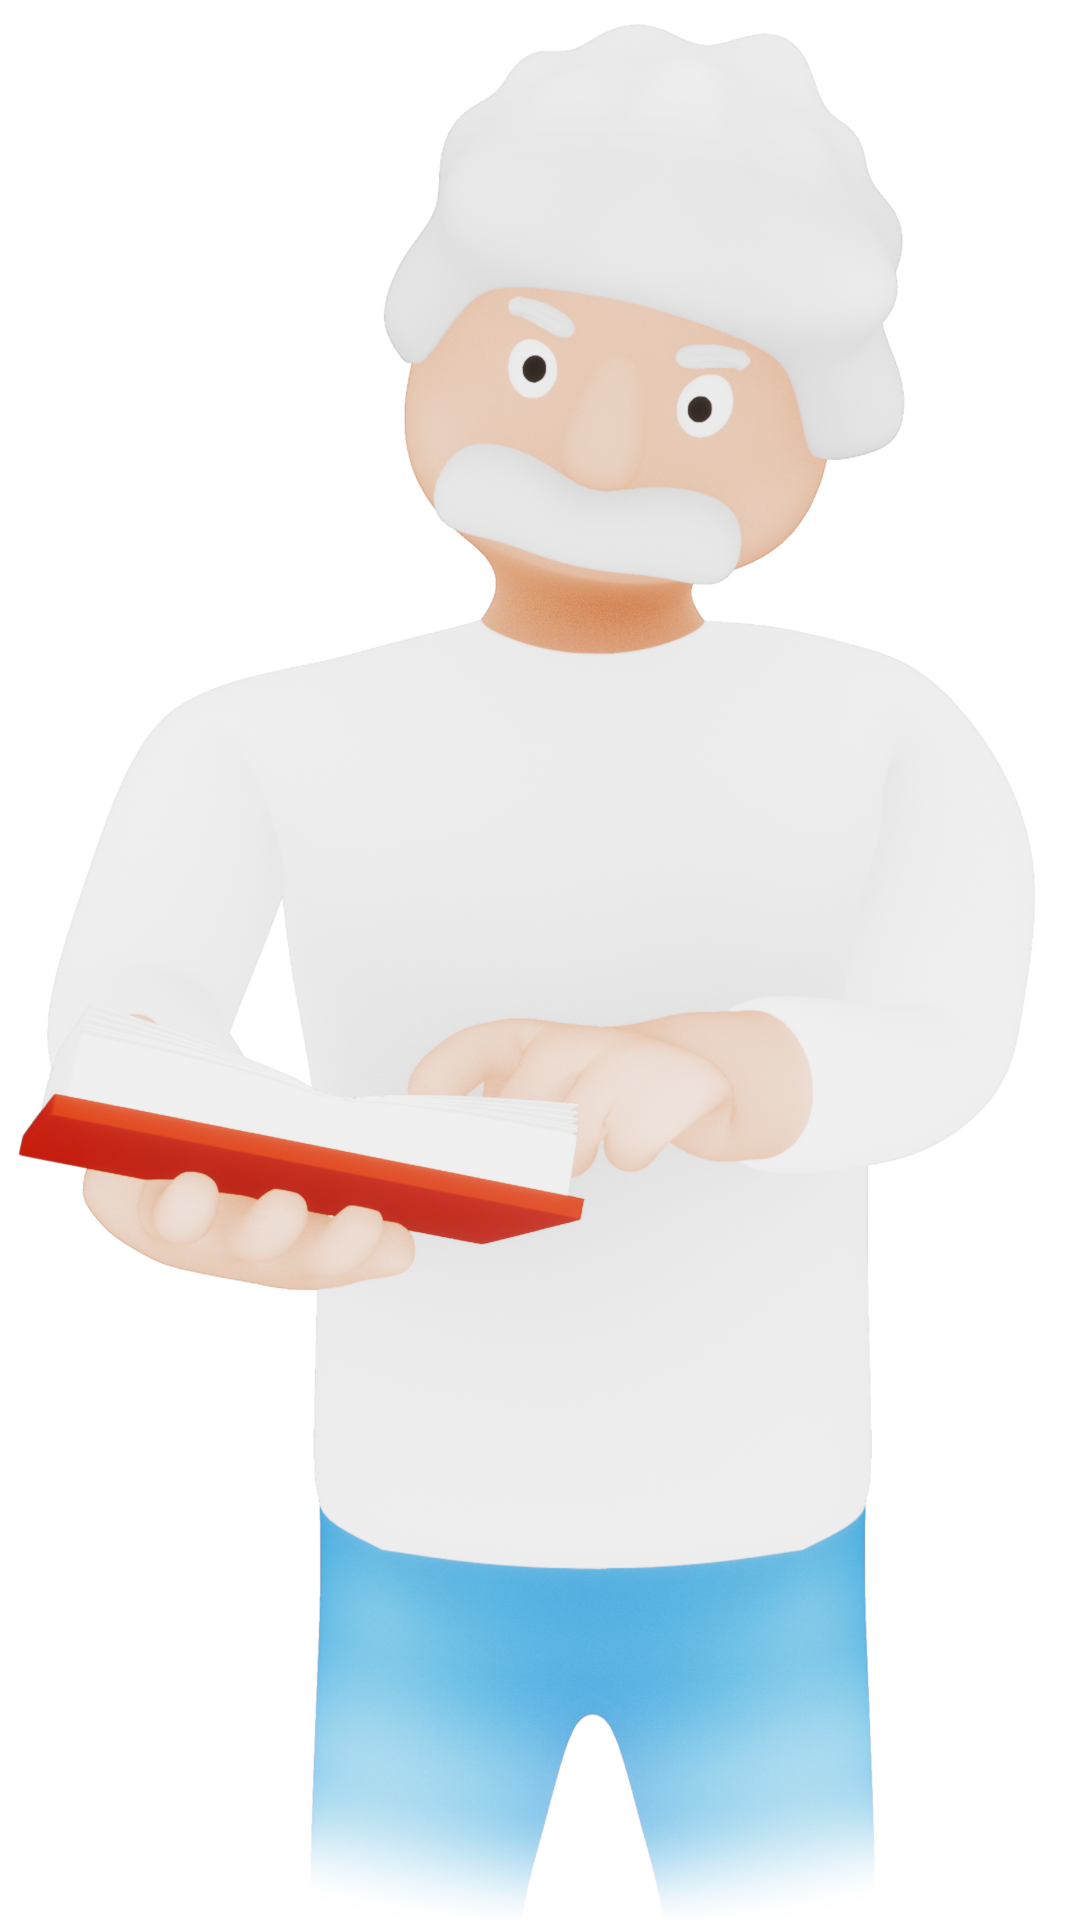
\includegraphics[width=1cm]{"icons/info.png"}};}}



%%%%% Exercise
% Define new colorbox
\newtcolorbox[auto counter]{exercise}[2][]{
% Add space before box and cener box
before=\bigskip\centering,
% Add space after the box
after=\bigskip,
% Activate enhanced mode of colorbox
enhanced,
% Create round corners
arc=15pt,
% Create blue frame
colframe=blender_blue,
% Craete blue background color
colback=blender_blue!5!white,
% Define Font of title (black font, sans-serife and large
fonttitle=\sffamily\bfseries\Large,
% Set title
title=Übung~\thetcbcounter,
% Define sharp corners
sharp corners,
% Set space in upper left corner 
leftupper=2.5cm,
% Overlay image
overlay={
  % Set anchor north-west
  \node[anchor=north west] 
    % Adjust position
    at ([xshift=10pt,yshift=-.65\baselineskip]frame.north west)
     % Add image
     {\includegraphics[width=1cm,height=1cm]{"icons/exercise.png"}};},
% Set round corners
rounded corners=northeast,
% Fix title to top of box
attach boxed title to top left,
% Define style of title
boxed title style={
    % Activate enhanced settings of title-field
    enhanced,
    % Set frame of title box
    colframe=blender_blue,
    % Set background of title box
    colback=blender_blue,
    % Set round-angle of title field
    arc=5pt,
    % Supress frame around title fileld
    bottomrule=0pt,
    rightrule=0pt,
    % Set sharp corners
    sharp corners,
    % Set round corners norh-east
    rounded corners=northeast,},
% Define stly of (emtpy) interior block
interior style={},
% Define style of frame
frame style={
    % Set colors
    color= cyan!5!white,
    fill=none},
% Align additional overlays
overlay unbroken and first={
    % Place text
    \node[anchor=west,font=\sffamily\bfseries,color=blue] 
    % Position text east of title and with large font
    at (title.east) {{\Large #2}};
    %
    \node[anchor=north west] 
    % Set position
    at ([xshift=10pt, yshift=-1.75\baselineskip]frame.north west)
      % Add image
     {\includegraphics[width=1.5cm]{"icons/exercise.png"}};},#1}



%%%%% Remember
% Define new colorbox
\newtcolorbox{remember}[1]{
% Add space before box and cener box
before=\bigskip\centering,
% Add space after the box
after=\bigskip,
% Activate enhanced mode of colorbox
enhanced,
% Create round corners
arc=10pt,
% Create gold frame
colframe=remember_gold,
% Craete gold background color
colback=remember_gold,
% Define Font of title (black font, sans-serife and large
fonttitle=\color{black}\sffamily\bfseries\Large,
% Set content 1 as title
title=#1,
% Add space before and after the title inside the box
title={\vspace{2.5mm}#1\vspace{2.5mm}},
% Set space in upper left corner 
leftupper=2.5cm,
% Set round corners
rounded corners,
% Fix title to top of box
attach boxed title to top,
% Define style of title
boxed title style={
    % Activate enhanced settings of title-field
    enhanced,
    % Set frame of title box
    colframe=remember_gold,
    % Set background of title box
    colback=remember_gold,
    % Set round-angle of title field
    arc=10pt,
    % Supress frame around title fileld
    bottomrule=0pt,
    rightrule=0pt
    },
  % Overlay image
  overlay={
    % Set anchor north-west
    \node[anchor=north west] 
      % Adjust position in relation to frame
      at ([xshift=10pt,yshift=-1.75\baselineskip]frame.north west)
        % Add image
       {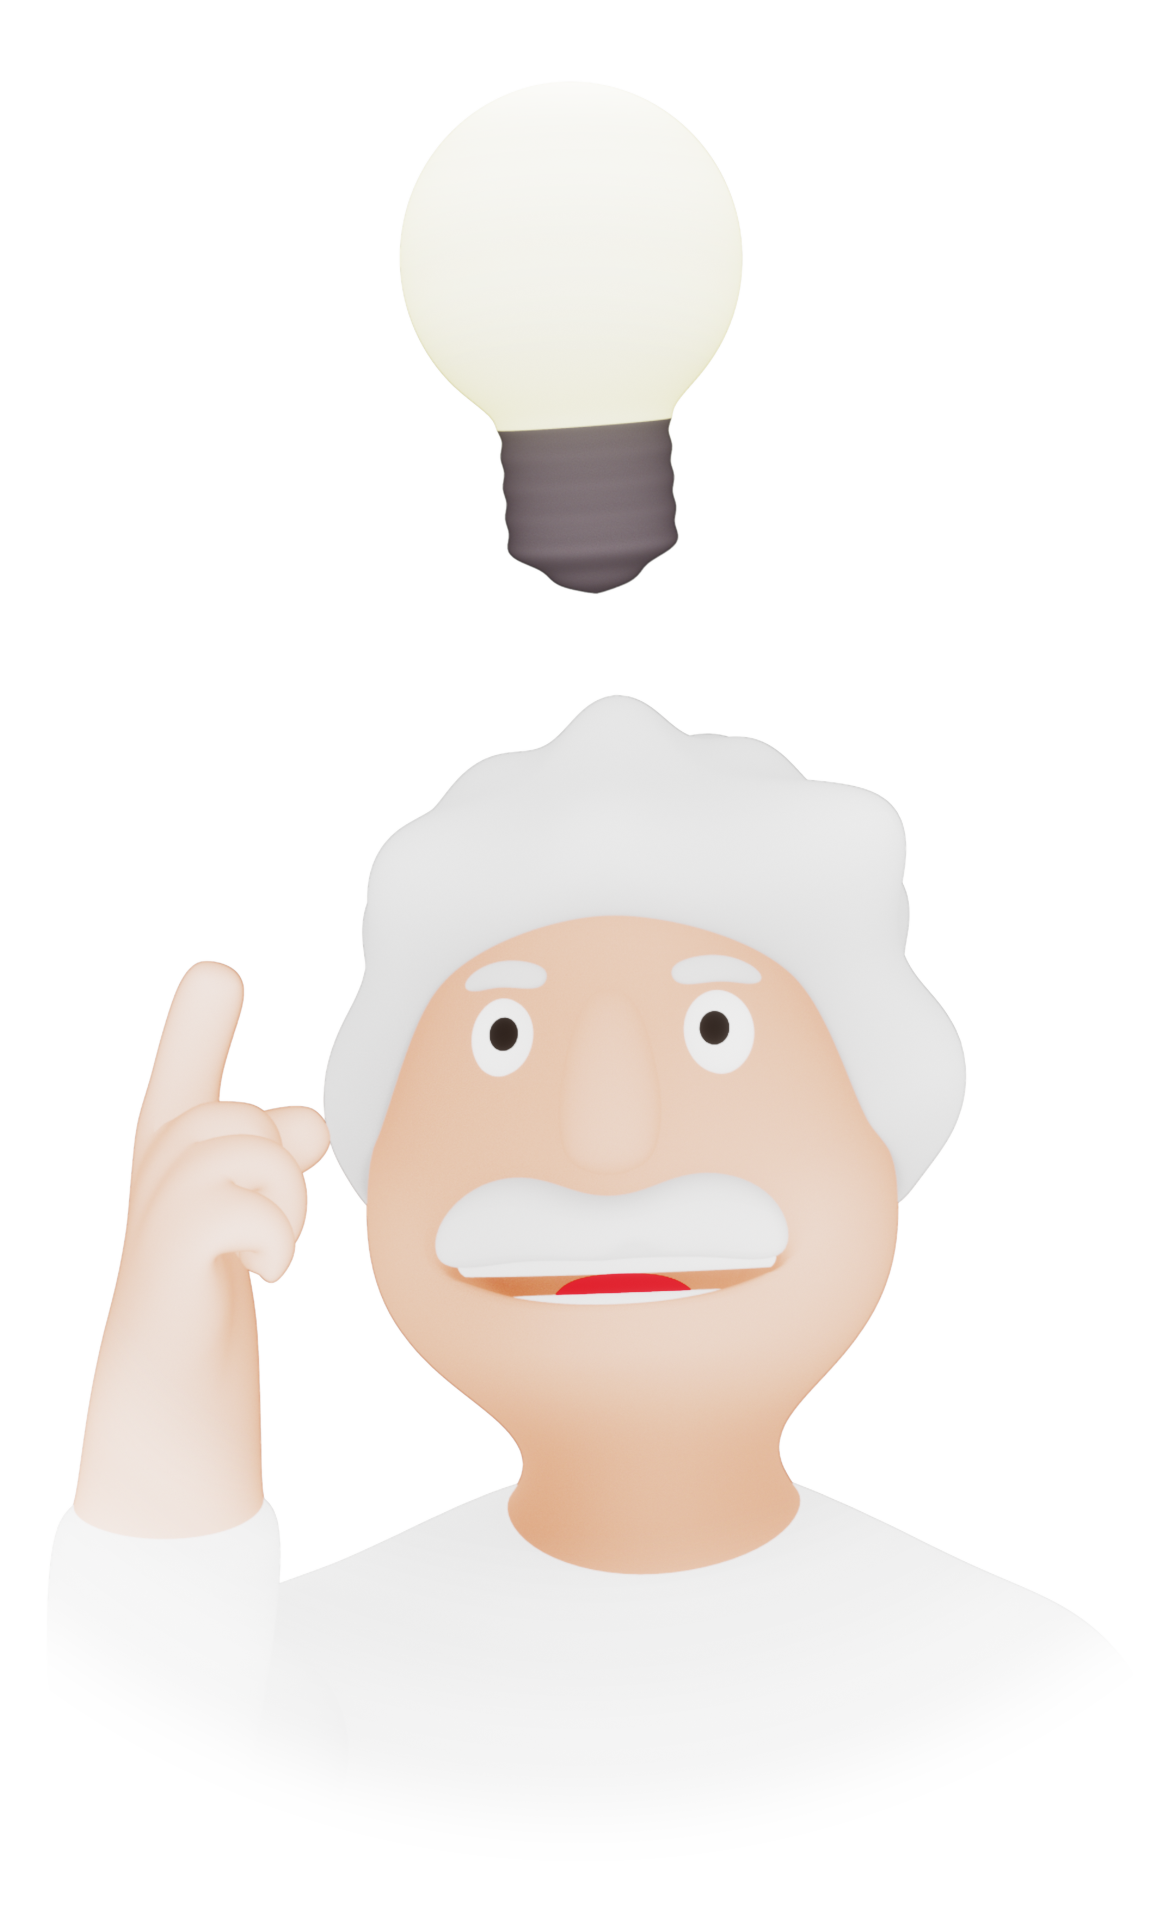
\includegraphics[width=1cm]{"icons/remember.png"}};}}
       


%%%%% Footer
\newcommand{\seitenzahlInFusszeile}{%
  \AddToShipoutPictureFG*{%
    \begin{tikzpicture}[remember picture, overlay]
      \ifodd\value{page}
        % Odd pages - box left
        \node[anchor=south west] at ([xshift=2.0cm]current page.south west) {%
          \raisebox{-0.15\baselineskip}{%
            \colorbox{blue_box}{%
              \parbox[c][1.25\baselineskip][t]{0.5cm}{%
                \vspace{0.28\baselineskip}% ← etwa 3mm nach unten
                \centering\color{white}\bfseries\small\thepage%
              }%
            }%
          }%
        };
      \else
        % even pages - box right
        \node[anchor=south east] at ([xshift=-2.0cm]current page.south east) {%
          \raisebox{-0.15\baselineskip}{%
            \colorbox{blue_box}{%
              \parbox[c][1.25\baselineskip][t]{0.5cm}{%
                \vspace{0.28\baselineskip}% ← etwa 3mm nach unten
                \centering\color{white}\bfseries\small\thepage%
              }%
            }%
          }%
        };
      \fi
    \end{tikzpicture}%
  }
}


\AtBeginShipout{%
  \ifthenelse{%
    \NOT\(\value{page}=1 \OR \value{page}=2\)%
  }{%
    \seitenzahlInFusszeile%
  }{}%
}
\renewcommand{\familydefault}{\sfdefault}
\newcommand{\kbd}[1]{\fbox{\texttt{#1}}}
\makeatletter
\@ifpackageloaded{caption}{}{\usepackage{caption}}
\AtBeginDocument{%
\ifdefined\contentsname
  \renewcommand*\contentsname{Inhaltsverzeichnis}
\else
  \newcommand\contentsname{Inhaltsverzeichnis}
\fi
\ifdefined\listfigurename
  \renewcommand*\listfigurename{Abbildungsverzeichnis}
\else
  \newcommand\listfigurename{Abbildungsverzeichnis}
\fi
\ifdefined\listtablename
  \renewcommand*\listtablename{Tabellenverzeichnis}
\else
  \newcommand\listtablename{Tabellenverzeichnis}
\fi
\ifdefined\figurename
  \renewcommand*\figurename{Abbildung}
\else
  \newcommand\figurename{Abbildung}
\fi
\ifdefined\tablename
  \renewcommand*\tablename{Tabelle}
\else
  \newcommand\tablename{Tabelle}
\fi
}
\@ifpackageloaded{float}{}{\usepackage{float}}
\floatstyle{ruled}
\@ifundefined{c@chapter}{\newfloat{codelisting}{h}{lop}}{\newfloat{codelisting}{h}{lop}[chapter]}
\floatname{codelisting}{Listing}
\newcommand*\listoflistings{\listof{codelisting}{Listingverzeichnis}}
\makeatother
\makeatletter
\makeatother
\makeatletter
\@ifpackageloaded{caption}{}{\usepackage{caption}}
\@ifpackageloaded{subcaption}{}{\usepackage{subcaption}}
\makeatother

\ifLuaTeX
\usepackage[bidi=basic]{babel}
\else
\usepackage[bidi=default]{babel}
\fi
\babelprovide[main,import]{ngerman}
% get rid of language-specific shorthands (see #6817):
\let\LanguageShortHands\languageshorthands
\def\languageshorthands#1{}
\ifLuaTeX
  \usepackage{selnolig}  % disable illegal ligatures
\fi
\usepackage{bookmark}

\IfFileExists{xurl.sty}{\usepackage{xurl}}{} % add URL line breaks if available
\urlstyle{same} % disable monospaced font for URLs
\hypersetup{
  pdflang={de},
  hidelinks,
  pdfcreator={LaTeX via pandoc}}


\author{}
\date{}

\begin{document}
\frontmatter


\mainmatter
\begin{titlepage}
  \thispagestyle{empty}

  % Background Image
  \AddToShipoutPictureBG*{%
    \put(0,0){%
      \parbox[b][\paperheight][c]{\paperwidth}{%
        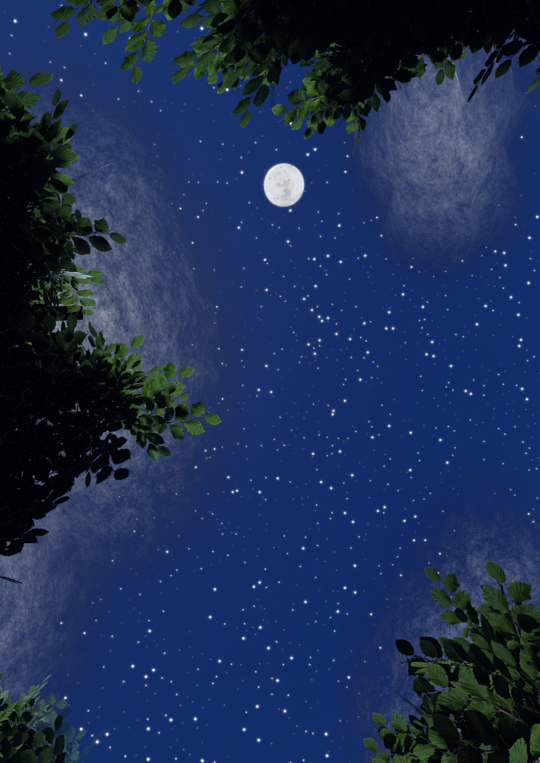
\includegraphics[width=\paperwidth,height=\paperheight]{icons/Title_Image.png}%
      }%
    }%
  }
  
  % Titlebox
  \begin{tikzpicture}[remember picture, overlay]
    \node[anchor=north west] at ([xshift=2.3cm,yshift=-9.3cm] current page.north west) {
      \begin{tikzpicture}
        % Box
        \shade[bottom color=orangeBottom, top color=orangeTop, opacity=0.45]
          (0,0) rectangle (16.51cm,3.91cm);
        % Text
        \node[anchor=west, text=white, align=left, font=\sffamily\bfseries\fontsize{24}{24}\selectfont]
          at (1.25cm,1.955cm) {
            Creating the World:\\
            Grafik, Design und Animation in 3D
          };
      \end{tikzpicture}
    };

  
    % Author-Box
    \node[anchor=north west] at ([xshift=2.3cm,yshift=-19.61cm] current page.north west) {
      \begin{tikzpicture}
        % Box
        \filldraw[fill=blue!90!cyan, opacity=0.35, draw=none]
          (0,0) rectangle (16.51cm,3.91cm);
        % Text
        \node[anchor=east, text=white, align=right, font=\sffamily\bfseries\fontsize{16}{18}\selectfont]
          at (16.31cm,1.955cm) {
            Michael Rihs\\
            Flurina Brodwolf\\
            Romina Schmid\\
            Fred Mast\\
          };
      \end{tikzpicture}
    };

  \end{tikzpicture}

  \newpage
\end{titlepage}

\clearpage
\thispagestyle{empty}

\chapter*{Creating the World:\protect\\Grafik, Design \& Animation}

\hfill\break

\vspace{1em}

\textbf{Version:} 2025\\
\textbf{Erstversion:} 2021\\

\textbf{Autoren:}\\
Michael Rihs\textsuperscript{*}\\
Flurina L. Brodwolf\\
Romina Schmid\\
Fred W. Mast\\
\strut \\
Abteilung für kognitive Psychologie, Wahrnehmung und Methodenlehre\\
Institut für Psychologie\\
Universität Bern\\

\vspace{1em}
\section*{Kontakt}

\begin{tabular}{@{}l}
\textbf{*Dr. Michael Rihs}\\
Institut für Psychologie \\
Fabrikstrasse 8 \\
3012 Bern \\
{michael.rihs@unibe.ch} \\
\end{tabular}

\newpage
\section*{Erstellung der Website}

Die Unterlagen zu diesem Buch sind auf der dazugehörigen Website
(\url{https://mrihs.github.io/Mrihs.Creating-the-World.github.io/}) zu
finden. Die Website wurde mit Hilfe von
\href{https://posit.co/download/rstudio-desktop/}{RStudio/Posit} und
\href{https://quarto.org}{Quarto} entwickelt. Die Website, sowie die
Unterrichts-Unterlagen sind im zur Website gehörigen GitHub Repository
(\url{https://github.com/Mrihs/Mrihs.Creating-the-World.github.io})
hinterlegt

\vspace{1em}
\section*{Lizenz}

Dieses Buch und die dazugehörige Website stellt eine offene
Bildungsressource (Open Educational Resource) dar. Sie darf frei
verwendet, bearbeitet und weitergegeben werden, sofern die Urheber
namentlich genannt und die Inhalte unter der Lizenz
\href{https://creativecommons.org/licenses/by-sa/4.0/deed.de}{CC BY-SA 4.0}
weitergegeben werden.

Abbildungen der Benutzeroberfläche von
\href{https://www.blender.org}{Blender} wurden als Screenshots erstellt
und unterliegen der Lizenzbedingungen von Blender.

\vspace{1em}
\section*{Danksagung}

Besonderer Dank geht an Rahel Steuri und Rebekka Borer, welche bei der
Adaption des Kurses im Jahre 2022 beteiligt waren. Weiterer Dank geht an
Aurégane Dévaud, welche die Erstellung der Website zum Buch unterstützt
hat.

\clearpage
\tableofcontents
\clearpage

\chapter*{Vorwort}

\hfill\break

\markboth{Vorwort}{}

Dieses Buch wurde für die Lehrveranstaltung ``Creating the World:
Grafik, Design \& Animation (inkl. Einführung in die 3D Modellierung mit
Blender) entwickelt. Der Kurs wurde erstmals im Jahr 2021 als
Methodenkurs für Masterstudierende der
philosophisch-humanwissenschaftlichen Fakultät der Universität
angeboten. Die Lehrveranstaltung wurde durch das Förderprogramm''Der
Mensch in der digitalen Transformation'' von der
philosophisch-humanwissenschaftlichen Fakultät gefördert. In der
Veranstaltung wurde der Prozess der Erstellung virtueller 3D-Objekte,
-Welten und Animationen vor dem Hintergrund aktueller Forschung
erläutert und durch praktische Beispiele veranschaulicht. Die
Studierenden erlernten die Inhalte praxisnah mithilfe der frei
zugänglichen Software Blender und erhielten dabei fundierte Einblicke in
die grundlegenden Merkmale von 3D-Objekten, -Welten und Animationen.

\section*{Hinweise zur Verwendung von Boxen}

Im Verlaufe des Buches werden verschiedene Boxen verwendet, um wichtige
Informationen hervorzuheben. Die Boxen haben folgende Bedeutung

\begin{tipp}{Tipps}
Diese Box kennzeichnet nützliche Tipps.
\vspace{2\baselineskip}
\end{tipp}

\begin{remember}{Merke...}
Diese Box kennzeichnet besonders wichtige Inhalte, die nicht vergessen werden sollten.
\vspace{2\baselineskip}
\end{remember}

\begin{exercise}{Übungen}
Diese Box kennzeichnet praktische Übungen.
\vspace{2\baselineskip}
\vspace{2\baselineskip}
\end{exercise}

\section*{Rückmeldung}

Haben Sie Rückmeldungen, Anregungen oder Fehler entdeckt? Diese können
gerne an Dr.~Michael Rihs (michael.rihs@unibe.ch) zurückgemeldet werden.

\chapter{Vorbereitung von Blender}\label{vorbereitung-von-blender}

\section{Installation von Blender}\label{installation-von-blender}

\marginnote{Installationsdatei herunterladen}

Um Blender auf einem Rechner zu installieren, muss das
Installationspaket von Blender auf dessen Website
\url{https://www.blender.org/} unter dem Reiter «Download»
heruntergeladen werden. Dort sollte bereits automatisch das
Betriebssystem des Rechners erkannt und die aktuellste Version angeboten
werden. Ansonsten lässt sich mittels eines Auswahlfeldes auch die
entsprechende Version auswählen.

\marginnote{Frühere Versionen von Blender}

Unter \url{https://www.blender.org/download/releases/} lassen sich zudem
frühere Versionen von Blender herunterladen. Dieser Kurs ist auf Blender
3.3 ausgerichtet, weshalb der Download dieser Version empfohlen wird.

\subsection{Mac}\label{mac}

\marginnote{Installationsdatei für Mac-User}

Mac-Benutzer wählen den Link mit der Endung «\emph{.dmg}». Abhängig vom
Computermodell gibt es zwei Versionen. Für Apple-Computer, welche Apples
hauseigenen Prozessor M1 eingebaut haben, wird die Version mit der
Endung «arm64.dmg» benötigt. Für die anderen Apple-Computer die Version
mit der Endung «\emph{x64.dmg}». Um herauszufinden, welcher
Prozessor/Chip im eigenen Apple-Gerät eingebaut ist, kann man im Menü
«\emph{Über diesen Mac}» (oben links beim Apfelsymbol zu finden)
nachschauen. Wenn Apples eigener Chip verbaut ist, wird «\emph{Chip
Apple M1}» aufgelistet. Wenn der Computer nicht über den M1-Chipf
verfügt, wird an dieser Stelle der Prozessor aufgeführt.

\marginnote{Installation}

Nach dem Download sollte das entsprechende .dmg-Paket geöffnet werden.
Anschliessend öffnet sich ein Fenster, dass die Blender-Software und den
Applikationsordner zeigt. Hier sollte nun die Blender-Software in den
Applikationsordner gezogen werden. Anschliessend ist die Installation
abgeschlossen.

\subsection{Windows}\label{windows}

\marginnote{Installation für Windows-User}

Windows-Benutzer können den Link mit der Endung «\emph{.msi}» auswählen.
Nach dem Download kann die Datei geöffnet werden und die Installation
konfiguriert werden.

\marginnote{Blender ohne Installation nutzen}

Es ist auch möglich, Blender ohne eine Installation zu verwenden --
hierfür muss der Link mit der Endung «\emph{.zip}» ausgewählt werden.
Nach dem Extrahieren der Dateien kann Blender über diesen Ordner
gestartet werden. Dadurch kann Blender auf ein externes Speichermedium
transferiert werden und an anderen Computern gestartet werden. Dies hat
allerdings einige Nachteile. Der Computer weiss dadurch etwa nicht, mit
welchem Programm er standardmässig die Dateien von Blender öffnen kann,
und Blender wird auch nicht unter den installierten Programmen
aufgelistet.

\begin{tipp}{Weiterführende Informationen}
Seit der Version 2.81 von Blender werden nur noch Computer mit einer 64-Bit-Architektur unterstützt. Microsoft unterstützt diese Systeme seit 2020 nicht mehr und auch andere Software-Entwickler haben den Support dieser Systeme eingestellt.
\end{tipp}

\section{Der erste Start von Blender}\label{der-erste-start-von-blender}

Beim ersten Start von Blender erscheint ein Quick-Setup-Menü, bei dem
einige Grundeinstellungen eingestellt werden können. Diese können in der
Regel so belassen werden, wie sie sind. Die folgenden Einstellungen
stehen zur Verfügung:

\begin{itemize}
\tightlist
\item
  \textbf{Language}: Hier kann die Sprache eingestellt werden.
\item
  \textbf{Shortcuts}: Hier können die Shortcut-Einstellungen ausgewählt
  werden. Dieser Kurs orientiert sich an der Default-Einstellung
  «\emph{Blender}».
\item
  \textbf{Select with}: Hier kann eingestellt werden, ob jeweils mit der
  linken oder der rechten Maustaste Objekte ausgewählt werden können.
  Dieser Kurs geht davon aus, dass eine Auswahl mit der linken Maustaste
  erfolgt.
\item
  \textbf{Spacebar}: Die Funktion der Leertaste kann drei verschiedenen
  Funktionen zugewiesen werden. Per Default wird die Leertaste
  verwendet, um Animationen zu starten (Option «\emph{Play}»).
  Allerdings kann sie auch der Option «\emph{Tools}» zugewiesen werden.
  Mittels der Einstellung «\emph{Search}» wird durch die Leertaste ein
  Suchfeld geöffnet, mit dem Befehle gesucht werden können. Für diesen
  Kurs spielt es keine grosse Rolle, welche Funktion der Leertaste
  zugewiesen wird. Die Befehlssuche ist allerdings sehr nützlich, kann
  aber alternativ auch mit der Taste \kbd{F3} geöffnet werden.
\item
  \textbf{Theme}: Hier kann das farbliche Layout von Blender angepasst
  werden. Grafiken in diesem Kurs wurden mit dem Theme «\emph{Blender
  Dark}» erstellt.
\end{itemize}

\section{Die Arbeitsoberfläche von
Blender}\label{die-arbeitsoberfluxe4che-von-blender}

\subsection{Das Willkommensfenster}\label{das-willkommensfenster}

\marginnote{Optionen im Willkommensfenster}

Blender begrüsst seine Nutzer mit einem Willkommensfenster. In diesem
Fenster werden die letzten geöffneten Projekte auf der rechten Seite
unter den «\emph{Recent Files}» aufgelistet. Auf der linken Seite des
Willkommensfenster kann unter «\emph{New File}» ein neues Projekt
erstellt werden. Dabei lässt sich die Art des Projekts bereits genauer
definieren. Je nach ausgewählter Projektart werden unterschiedliche
Ansichtsvorlagen geladen.

\begin{figure}

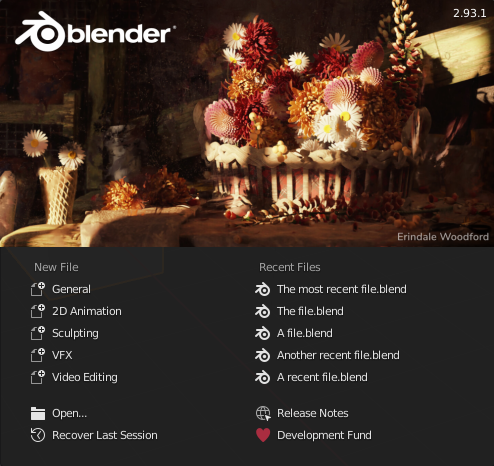
\includegraphics{Chapters/Images/Chapter_1/1_1_Welcome_Screen.png}

\caption{\label{fig-1_1}Willkommensfenster}

\end{figure}%

\marginnote{Auswahl von Ansichtsvorlagen}

Zu den möglichen Ansichtsvorlagen gehören:

\begin{itemize}
\tightlist
\item
  \textbf{General}: Öffnet eine Standardvorlage für das Bearbeiten von
  3D-Objekten.
\item
  \textbf{2D Animation}: Öffnet eine Vorlage zum Erstellen von
  2D-Animationen.
\item
  \textbf{Sculpting}: Öffnet eine Vorlage, welche für das Sculpting von
  Objekten geeignet ist. Dabei werden Objekte anhand von Pinseln direkt
  in ihrer Form verändert.
\item
  \textbf{VFX}: Öffnet eine Vorlage für die Erstellung visueller Effekte
  (VFX), beispielsweise in Videos.
\item
  \textbf{Video Editing}: Öffnet eine Vorlage zum Bearbeiten von Videos.
\end{itemize}

\marginnote{Fokus auf «General»}

Dieser Kurs wird sich auf die 3D-Modellierung fokussieren. Deshalb wird
jeweils die Ansichtsvorlage «\emph{General}» verwendet. Diese Vorlage
ist so generell, dass sie im Hintergrund schon geladen ist, während das
Willkommensfenster dargestellt wird. Deshalb ist es auch möglich,
einfach ausserhalb des Willkommensfensters zu klicken. Dadurch
verschwindet das Willkommensfenster und die General-Vorlage, die bereits
im Hintergrund besteht, wird sichtbar.

\subsection{Die verschiedenen Areale beim
General-Projekt}\label{die-verschiedenen-areale-beim-general-projekt}

\marginnote{Default Editoren}

Die verschiedenen Werkzeuge, welche Blender anbietet, sind innerhalb
verschiedener Editoren aufzufinden. Diese Editoren werden als separate
und austauschbare Areale in Blender dargestellt. Beim Start eines neuen
Projekts (mit der Vorlage General) ist die Ansicht in vier Areale
unterteilt:

\begin{itemize}
\tightlist
\item
  \textbf{3D Viewport}: Überspannt von der oberen linken Ecke den
  grössten Teil des Bildschirms.
\item
  \textbf{Outliner}: Befindet sich in der oberen rechten Ecke.
\item
  \textbf{Properties}: Befindet sich in der unteren rechten Ecke.
\item
  \textbf{Timeline}: Befindet sich links am unteren Rand.
\end{itemize}

Gerade der 3D-Viewport, der Outliner und die Properties sind für das
Erstellen von 3D-Objekten mit Blender von hoher Bedeutung. Die Timeline
wird bei Animationen verwendet.

\begin{figure}

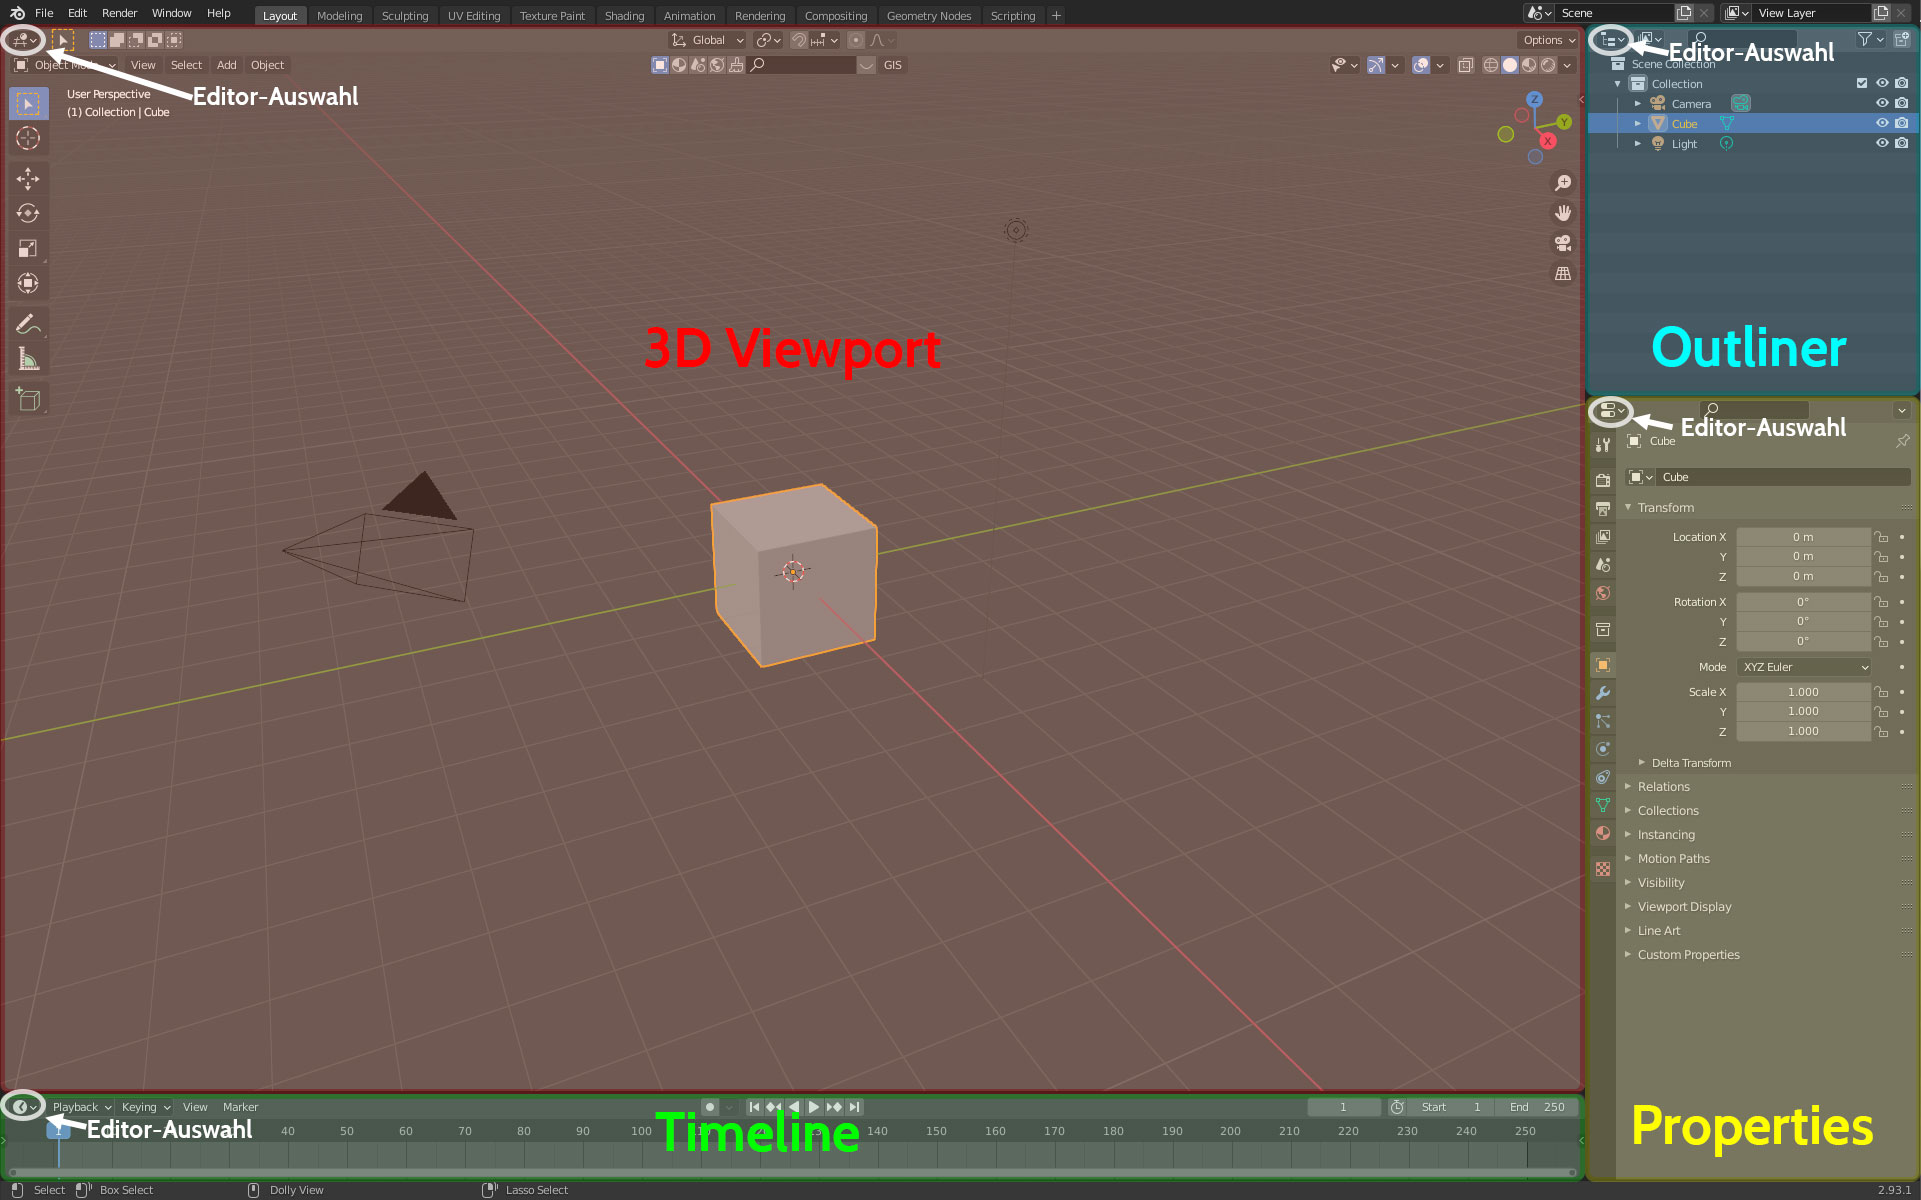
\includegraphics{Chapters/Images/Chapter_1/1_2_Default_Areal.jpg}

\caption{\label{fig-1_2}Default-Aufteilung der Arbeitsbereiche.}

\end{figure}%

\section{Übersicht über die Editor-Fenster von
Blender}\label{uxfcbersicht-uxfcber-die-editor-fenster-von-blender}

\marginnote{Editoren austauschen}

In jedem Editor-Areal befindet sich in der linken oberen Ecke eine
Schaltfläche. Durch das Drücken dieser Schaltfläche wird ein
Dropdown-Menü geöffnet. Darin sind alle verfügbaren Editoren
aufgelistet. Indem ein anderer Editor ausgetauscht wird, wechselt die
Anzeige in diesem Areal zu dem ausgewählten Editor.

\begin{figure}

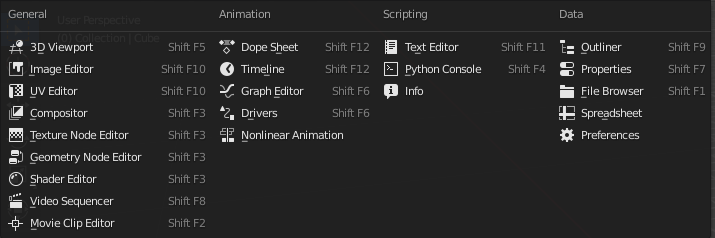
\includegraphics{Chapters/Images/Chapter_1/1_3_Editor_Select.png}

\caption{\label{fig-1_3}Die Auswahl an verschiedenen Editoren, welche
Blender standardmässig mit sich bringt.}

\end{figure}%

\subsection{3D Viewport}\label{d-viewport}

\marginnote{«General» Edito-ren}

Der 3D-Viewport stellt die bearbeiteten Szenen und die dazugehörigen
3D-Objekte dar. Er bietet die Möglichkeit zur direkten Interaktion mit
diesen Objekten und ist für das Modellieren von Objekten essenziell. Bei
der Arbeit mit 3D-Objekten ist es der wichtigste Editor.

\subsection{Image Editor}\label{image-editor}

Anhand des Image-Editors können 2D-Grafiken betrachtet und bearbeitet
werden. Gerenderte Bilder werden ebenfalls in diesem Editor angezeigt.

\subsection{UV Editor}\label{uv-editor}

Der UV-Editor wird verwendet, um den Flächen von Objekten eine bestimmte
Position auf einer Textur (sogenannte UVs) zuzuweisen oder dessen
Zuweisung zu betrachten.

\subsection{Compositor}\label{compositor}

Mithilfe des Compositors lassen sich Bilder, welche beim Rendern
erstellt werden, nachträglichen Bearbeitungen unterziehen. Auch externe
Bilder können hier bearbeitet werden. Die Bearbeitung erfolgt mittels
einer visuellen Programmiersprache.

\subsection{Texture Node Editor}\label{texture-node-editor}

Mithilfe des Texture-Node-Editors können Texturen anhand einer visuellen
Programmiersprache erstellt werden. Dieser Editor wird allerdings in
Zukunft durch andere Bearbeitungsoptionen ersetzt.

\subsection{Geometry Node Editor}\label{geometry-node-editor}

Der Geometry-Node-Editor ermöglicht das Bearbeiten von Objekten mittels
einer visuellen Programmiersprache. Innerhalb dieses Editors erfolgt
dabei die Programmierung der geometrischen Figuren, während die
Darstellung der Figuren im 3D-Viewport erfolgt. Bei den Geometry Nodes
handelt es sich um eine neue Funktion von Blender.

\subsection{Shader Editor}\label{shader-editor}

Mithilfe des Shader-Editors können die Materialien, welche einem
dreidimensionalen Objekt zugewiesen sind, bearbeitet werden. Dadurch
lässt sich bearbeiten, wie die Oberfläche eines Objektes aussieht. Die
Bearbeitung erfolgt hier mittels einer visuellen Programmiersprache.
Innerhalb dieses Editors werden lediglich die Einstellungen für die
Materialien gemacht. Um die Auswirkungen der Materialien zu sehen, wird
der 3D-Viewport verwendet.

\subsection{Video Sequencer}\label{video-sequencer}

Mithilfe des Video-Sequencers können Videoaufnahmen bearbeitet werden.
Dieser Editor verfügt zusätzlich über eine Vorschau-Option, mit der sich
die Videos direkt betrachten lassen.

\subsection{Movie Clip Editor}\label{movie-clip-editor}

Der Movie-Clip-Editor ermöglicht das Erfassen von Bewegungen in Filmen,
sodass diese Bewegungen beispielsweise auch auf 3D-Objekte angewendet
werden können. Zudem lassen sich hier auch Videos maskieren.

\subsection{Dope Sheet}\label{dope-sheet}

\marginnote{Editoren für Animationen}

Das Dope-Sheet stellt einzelne Animationspunkte eines Projektes in einem
zeitlichen Ablauf tabellarisch dar. Dies basiert auf der früher
angewendeten Planung von handgezeichneten Animationen.

\subsection{Timeline}\label{timeline}

Die Timeline stellt einen zeitlichen Verlauf von Animationen dar. Für
die ausgewählten Objekte wird hier durch Punkte dargestellt, wann eine
Animation im Zeitstrang starten oder enden soll. Zudem befindet sich
hier auch eine Schaltfläche, um Animationen abspielen zu lassen.

\subsection{Graph Editor}\label{graph-editor}

Mittels des Graph-Editors können Animationen über die Zeit hinweg
verfeinert werden. Hierfür werden die einzelnen Animationen mittels
Grafen dargestellt. Durch eine Veränderung dieser Grafen wird die
Animation verfeinert.

\subsection{Drivers}\label{drivers}

Der Driver-Editor ermöglicht es, Animationen gezielt zu steuern. Dabei
können die Eigenschaften eines Objektes verwendet werden, um ein anderes
Objekt zu steuern.

\subsection{Nonlinear Animation}\label{nonlinear-animation}

Mittels des Editors für nonlineare Animationen können Animationen
ausserhalb eines linearen Ablaufes gesteuert werden. Dies kommt etwa bei
komplexeren Veränderungen von Szenen zum Einsatz.

\subsection{Text Editor}\label{text-editor}

\marginnote{Editoren für Programmier-Skripte}

Im Text-Editor können Textdokumente eingesehen und erstellt werden.
Diese Textdokumente können auch verwendet werden, um mittels der
Programmiersprache Python Funktionen für Blender zu verfassen. Zudem
können im Text-Editor auch direkt Programmfunktionen in Textdokumenten
ausgeführt werden.

\subsection{Python Console}\label{python-console}

Anhand der Python-Konsole lassen sich Codes in der Programmiersprache
von Python eingeben. Blender führt diese Codes anschliessend aus.

\subsection{Info}\label{info}

Im Info-Editor werden durchgeführte Aktionen in der
Python-Programmiersprache nacheinander aufgelistet. Hier lassen sich
auch Fehlermeldungen und Warnungen nachträglich einsehen.

\subsection{Outliner}\label{outliner}

\marginnote{«Data»-Editoren}

Im Outliner werden alle Daten, welche sich in einer Blender-Datei
befinden, aufgelistet. Hier lassen sich Objekte innerhalb einer Szene
auswählen oder in Ordnerstrukturen (sogenannten Collections) anordnen
und gruppieren.

\subsection{Properties}\label{properties}

Im Properties Editor lassen sich eine Reihe von Einstellungen machen. Es
umfasst neben Einstellungen zu einem aktuell ausgewählten Objekt auch
Einstellungen zum Rendern, zur Szenengestaltung oder zu physikalischen
Simulationen.

\subsection{File Browser}\label{file-browser}

Mithilfe des File-Browsers lassen sich Dateien auf dem Computer
darstellen und suchen. Dadurch können Dokumente direkt in die Szene
hineingezogen werden, ohne dass Blender minimiert werden muss. Zudem
können hier auch Dateien abgespeichert werden.

\subsection{Spreadsheet}\label{spreadsheet}

Mithilfe des Spreadsheets lassen sich alle Datenpunkte eines Objektes
mitsamt deren Positionen in der 3D-Welt angeben. Nebst den Punkten
können auch die Positionen der verschiedenen Kanten und Flächen von
Objekten angezeigt werden.

\subsection{Preferences}\label{preferences}

Unter den Preferences lassen sich die Einstellungen von Blender
bearbeiten. Die Preferences können auch unter «\emph{Edit \textbar{}
Preferences}» geöffnet werden.

\section{Vorgefertigte
Editor-Anordnungen}\label{vorgefertigte-editor-anordnungen}

\marginnote{Schnelle Auswahl von Editoren mittels Editor-Anordnungen}

In der Menüleiste sind für verschiedene Arbeitsschritte bei der
3D-Modellierung bereits vorgefertigte Ansichtsoptionen verfügbar. Durch
einen Klick auf den Reiter «\emph{Texture Paint}» wird beispielsweise
eine Anordnung gezeigt, welche ideal dafür ist, um ein Objekt mit einer
Textur zu bemalen. In diesem Falle wird beispielsweise nebst dem
3D-Viewport auch der Image Editor geöffnet. Mittels der Registerkarte
«+» können zudem weitere Editor-Anordnungen basierend auf einer Vorlage
für die Schnellauswahl hinzugefügt werden.

\section{Neuanordnen der
Editor-Areale}\label{neuanordnen-der-editor-areale}

\marginnote{Grösse der Edito-ren verändern}

Die einzelnen Editor-Fenster können nicht nur beliebig ausgetauscht
werden, sondern auch nach eigenem Belieben vergrössert oder verkleinert
werden. In den Abgrenzungsbereichen zwischen den Fenstern verändert sich
der Mauszeiger. Von dort aus lassen sich die Editor-Areale durch Hin-
und Herziehen vergrössern oder verkleinern.

\marginnote{Neue Editoren öffnen}

In den Ecken der einzelnen Editor-Fenster gibt es zudem die Möglichkeit,
durch Ziehen der Ecke in eine Richtung das Fenster in zwei Editoren
aufzuteilen. Wenn dabei gleichzeitig die \kbd{Shift}-Taste gedrückt
wird, wird derselbe Editor in einem neuen, einzelnen Fenster geöffnet.

\marginnote{Editor-Areal schliessen}

Um ein Editor-Fenster zu schliessen, wird jeweils ein anderes
Editor-Fenster über das zu schliessende Fenster gezogen. Dadurch werden
die beiden Fenster verbunden. Um zwei Fenster zu verbinden, wird eine
der beiden Ecken, welche sich zwischen den beiden Fenstern befindet,
ausgewählt und das zu behaltende Fenster über das zu entfernende Fenster
gezogen. Dies ist manchmal etwas knifflig, da die Aktion ähnlich zum
Öffnen von neuen Fenstern ist.

Übung 1: Editor-Auswahl

\textbf{Übung 1.1}

Ordnen Sie die Arbeitsoberfläche entsprechend der nachfolgenden
Abbildung an.

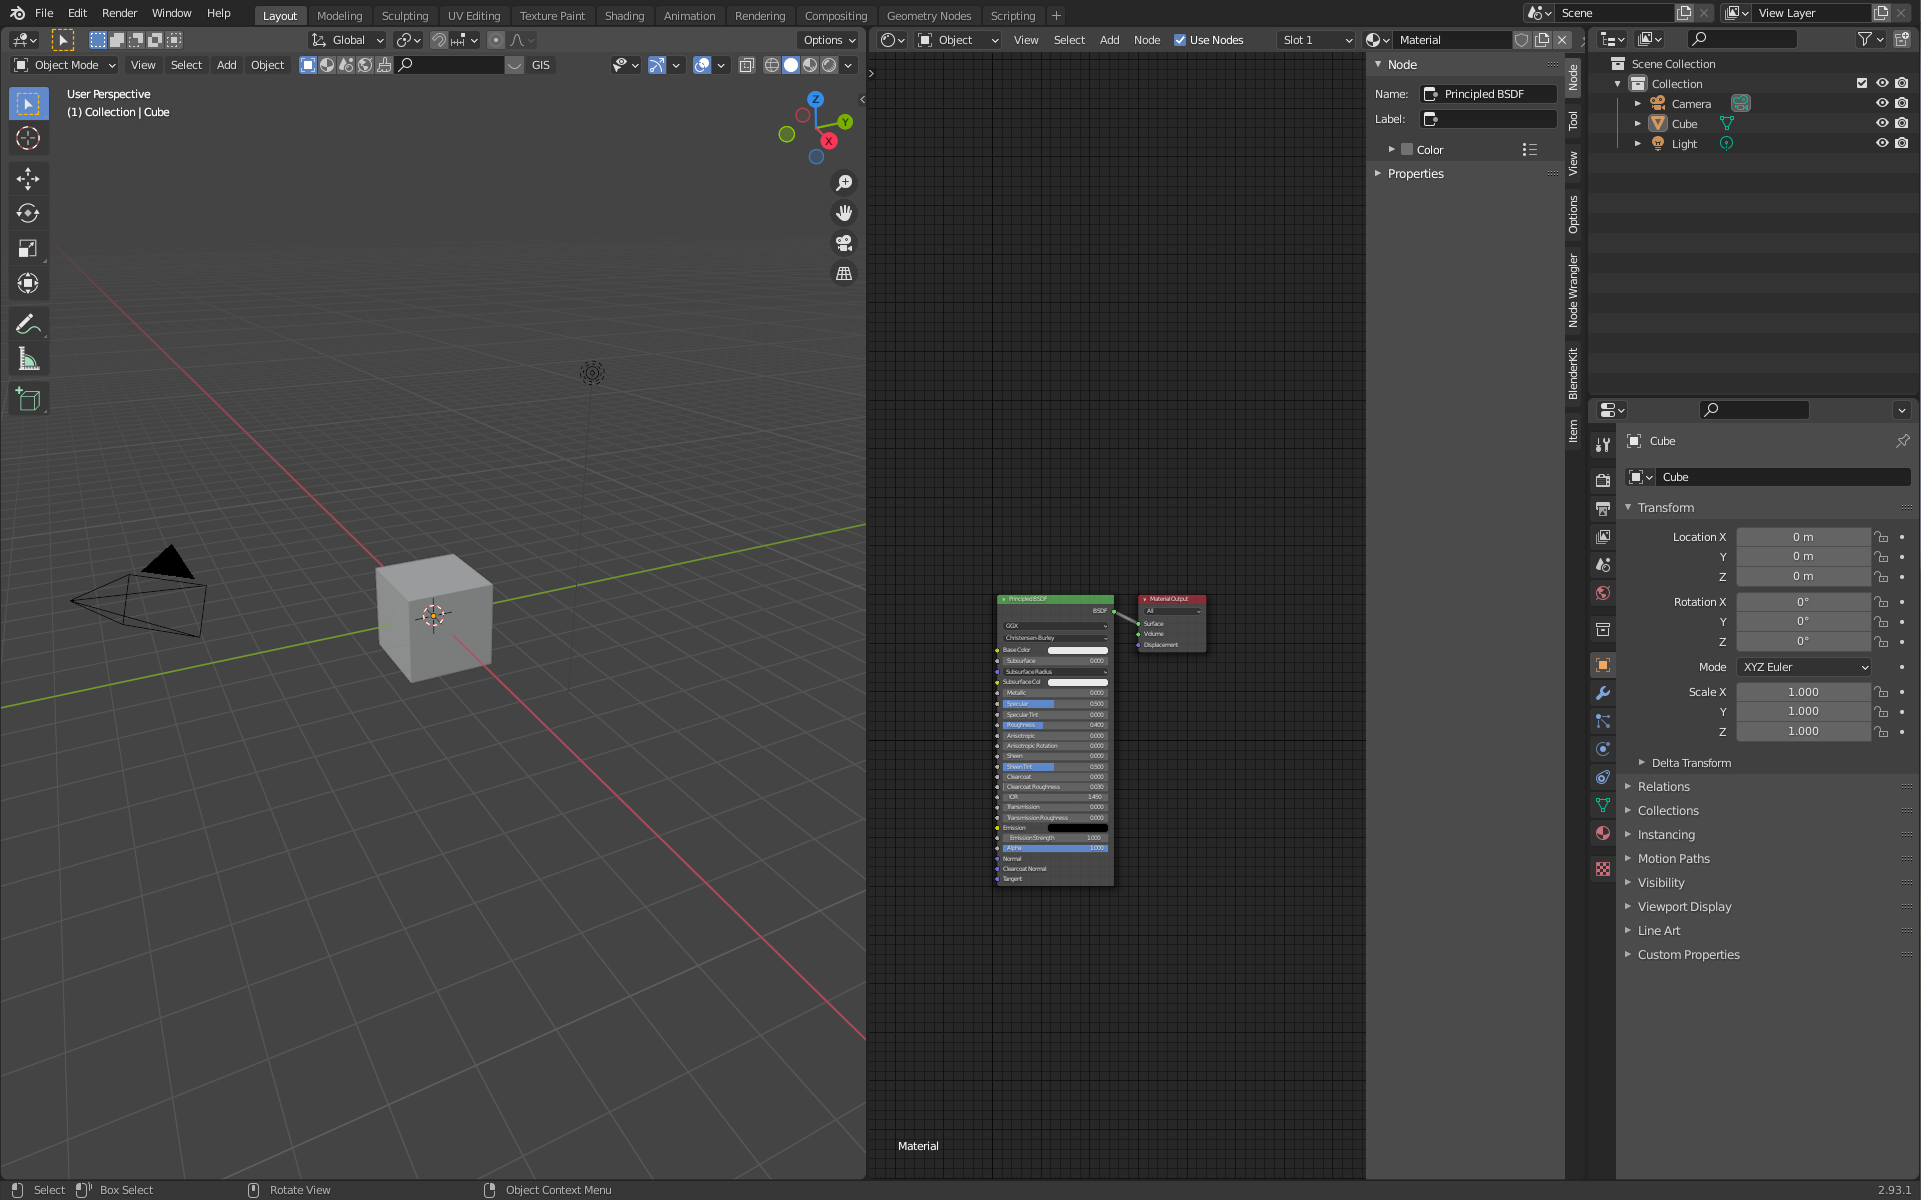
\includegraphics{Chapters/Images/Chapter_1/Exercise_1_1.png}\hfill

\textbf{Übung 1.2}

Ordnen Sie die Arbeitsoberfläche entsprechend der nachfolgenden
Abbildung an.

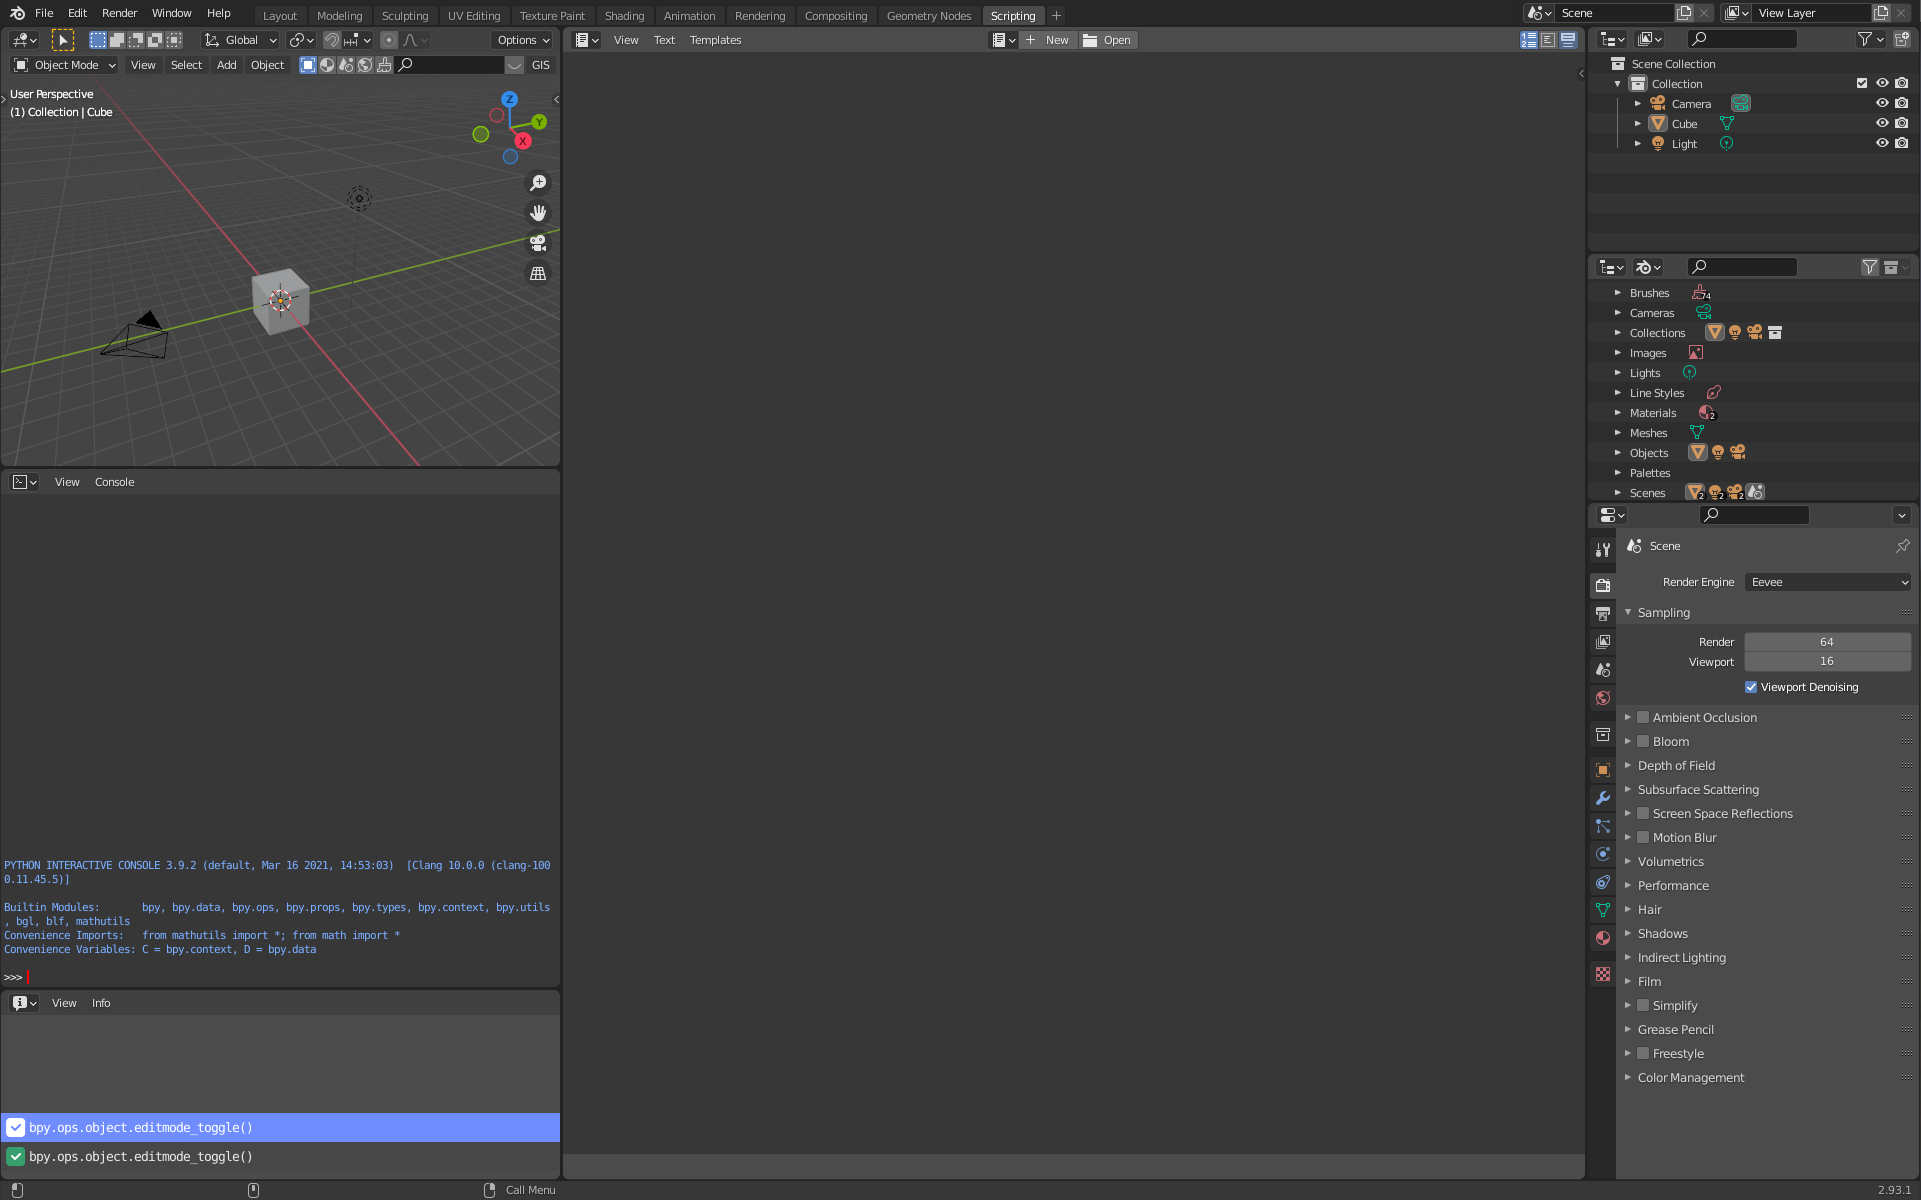
\includegraphics{Chapters/Images/Chapter_1/Exercise_1_2.png}\hfill

\chapter{Die Arbeitsoberfläche des
3D-Viewports}\label{die-arbeitsoberfluxe4che-des-3d-viewports}

\marginnote{Funktion des 3D-Viewports}

Der 3D-Viewport stellt eine der wichtigsten Arbeitsoberflächen in
Blender dar. In ihm werden die 3D-Objekte sowie die Szenen, in denen sie
integriert werden, angezeigt. Zudem werden im 3D-Viewport eine Reihe
anderer Einstellungen dargestellt, welche in anderen Editoren
konfiguriert werden können. Die Bearbeitung der grundlegenden Struktur
von 3D-Objekten erfolgt in der Regel direkt im 3D-Viewport. Der
Arbeitsbereich des 3D-Viewports lässt sich in verschiedene Areale
aufteilen, welche nachfolgend genauer betrachtet werden.

\section{Toolbar}\label{toolbar}

\marginnote{Toolbars}

Die Toolbar befindet sich auf der linken Seite der 3D-View. Allerdings
sind Toolbars auch in anderen Editoren anzutreffen. Die Toolbars lassen
sich jeweils mit der Taste \kbd{T} ein- und ausblenden. Da es auch im
3D-Viewport verschiedene Bearbeitungsmöglichkeiten gibt, variieren die
Elemente in der Toolbar abhängig vom Bearbeitungsmodus. Diese sind
entweder per Mausklick über diese Toolbar oder mithilfe von
Tastenkombinationen aufrufbar. In diesem Kurs wird vor allem auf
Tastenkombinationen verwiesen, wenn Operationen durchgeführt werden.

\section{Sidebar}\label{sidebar}

\marginnote{Sidebars}

Die Sidebar befindet sich auf der rechten Seite des Viewport-Displays,
muss allerdings noch mit der Taste \kbd{N} geöffnet werden. Mit dieser
Taste lässt sich die Sidebar ebenfalls wieder verbergen. Die Sidebar ist
auch in anderen Editoren anzutreffen und wird dort ebenfalls mit der
Taste\kbd{N} ein- und ausgeblendet. Die Sidebar ist zudem anhand von
Registerkarten in zusätzliche Kategorien eingeordnet. Unter dem Register
«\emph{Item}» können etwa Einstellungen zum aktuell ausgewählten Objekt
betrachtet und verändert werden, im Register «\emph{Tool}» können
Einstellungen zum aktuell ausgewählten Werkzeug verfeinert werden und
unter dem Register «\emph{View}» können Einstellungen zur Ansicht
betrachtet und verfeinert werden.

\section{Header}\label{header}

Im Header sind zusätzliche Einstellungen aufzufinden. Diese können nicht
nur zwischen den einzelnen Editoren variieren, sondern auch zwischen den
einzelnen Bearbeitungsmodi inner-halb der 3D-View.

\subsection{Aktions-Einstellungen}\label{aktions-einstellungen}

In der oberen linken Ecke, direkt neben dem Bedienfeld für die Auswahl
des Editors, befinden sich Einstellungsmöglichkeiten, welche basierend
auf der aktuell durchgeführten Aktion verfeinert werden können.

\begin{figure}

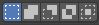
\includegraphics{Chapters/Images/Chapter_2/2_1_Actions_Parameters.png}

\caption{\label{fig-2_1}Aktions-Einstellungen am Beispiel der Auswahl.}

\end{figure}%

\subsection{Erweiterte Hilfsmittel zur
Bearbeitung}\label{erweiterte-hilfsmittel-zur-bearbeitung}

\marginnote{Hilfsmittel zur Bearbeitung von Objekten}

In der Mitte des Headers befinden sich eine Reihe von erweiterten
Einstellungen, welche bei der Objektbearbeitung als Hilfsmittel
verwendet werden können. Hierzu gehört beispielsweise die proportionale
Bearbeitung von Objekten oder das Festlegen von Bezugspunkten für
Transformationen. Diese Hilfsmittel werden in einem späteren Kapitel
ausführlich behandelt.

\begin{figure}

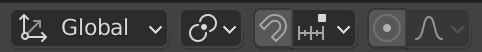
\includegraphics{Chapters/Images/Chapter_2/2_2_Extended_helper.png}

\caption{\label{fig-2_2}Erweiterte Hilfsmittel.}

\end{figure}%

\subsection{Bearbeitungsmodus}\label{bearbeitungsmodus}

\marginnote{Auswahl des Bearbeitungsmodus}

In der Zeile unterhalb des Headers befindet sich links das Menü zur
Auswahl des Bearbeitungsmodus. Dabei wird definiert, wie das aktuelle
Objekt bearbeitet werden soll. So kann beispielsweise im Object-Mode das
Objekt als Ganzes bearbeitet werden, während im Edit-Mode die Struktur
des Objektes bearbeitet werden kann.

\begin{figure}


\includegraphics{Chapters/Images/Chapter_2/2_3_Edit_Mode_Choice.png}

\caption{\label{fig-2_3}Auswahl des Bearbeitungsmodus.}

\end{figure}%

\subsection{Anzeige-Optionen}\label{anzeige-optionen}

\marginnote{Anzeige-Optionen}

In der rechten oberen Ecke befinden sich Optionen zur Darstellung der
Objekte in der 3D-View. Diese umfassen:

\begin{itemize}
\tightlist
\item
  View Object Types
\item
  Show Gizmo
\item
  Show Overlay
\item
  Toggle X-Ray
\item
  Viewport Shading
\end{itemize}

\subsubsection{View Object Types}\label{view-object-types}

\marginnote{Ein- und Ausblen-den von Objektarten}

Hier lassen sich verschiedene Arten von Objekten alle gemeinsam
innerhalb einer Szene verstecken, indem das Auge zu der entsprechenden
Objektart abgewählt wird. Durch das Abwählen des Auges neben dem
Objekttyp «\emph{Camera}» werde etwa alle Kameras aus der Szene
unsichtbar gemacht. Die Objekte sind allerdings noch vorhanden und
weisen immer noch dieselbe Funktion auf -- sie werden lediglich nicht
mehr im 3D-Viewport angezeigt. Neben dem Auge lässt sich zudem anhand
der Schaltfläche mit einem abgebildeten Cursor einstellen, dass die
entsprechenden Objektarten nicht mehr auswählbar sind.

\begin{figure}


\includegraphics{Chapters/Images/Chapter_2/2_4_Icon_Viewobjecttypes.png}

\caption{\label{fig-2_4}View Object Types.}

\end{figure}%

\subsubsection{Show Gizmo}\label{show-gizmo}

\marginnote{Navigations-Tools ein- und ausblen-den}

Innerhalb dieser Option lassen sich in der oberen rechten Ecke Tools zur
Navigation mittels der Kamera ein- und ausblenden. Zudem kann hier die
Darstellung eines Gizmos bei der aktuellen Auswahl aktiviert werden.
Dieses Gizmo kann verwendet werden, um Objekte mittels der Maus zu
rotieren, zu skalieren oder zu bewegen.

\begin{figure}

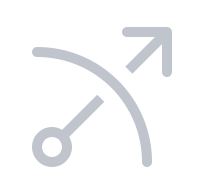
\includegraphics{Chapters/Images/Chapter_2/2_5_Icon_Show_Gizmos.png}

\caption{\label{fig-2_5}Show Gizmo.}

\end{figure}%

\subsubsection{Show Overlays}\label{show-overlays}

\marginnote{Orientierungsobjekte im Viewport ein- und ausblenden}

Durch die Deaktivierung der Viewport-Overlays wird im 3D-Viewport die
Ansicht bestimmter Hilfsmittel (beispielsweise die Achsen oder die
Markierung der aktuellen Auswahl) ausgeschal-tet. Im Dropdown-Menü lässt
sich zudem die Darstellung von einzelnen Hilfsmitteln individuell an-
und abwählen.

\begin{figure}


\includegraphics{Chapters/Images/Chapter_2/2_6_Icon_Showoverlays.png}

\caption{\label{fig-2_6}Show Overlays.}

\end{figure}%

\subsubsection{Toggle X-Ray}\label{toggle-x-ray}

\marginnote{Röntgenblick ein- und ausschalten}

Wenn die Schaltfläche «Toggle X-Ray» ausgewählt ist, erweitert sich die
Ansicht von Objekten, sodass durch sie hindurchgesehen werden kann. Dies
ermöglicht es etwa, dass auch ein Objekt, welches hinter einem anderen
Objekt verborgen liegt, betrachtet werden kann. Wenn diese Option
aktiviert ist, können zudem die verborgenen Objekte mittels eines
Mausklicks angewählt werden. Die Schaltfläche kann auch mit den Tasten
\kbd{Alt} + \kbd{Z} ein- und ausgeschaltet werden.

\begin{figure}


\includegraphics{Chapters/Images/Chapter_2/2_7_Icon_Xray.png}

\caption{\label{fig-2_7}Toggle X-Ray.}

\end{figure}%

\subsubsection{Viewport Shading}\label{viewport-shading}

\marginnote{Art der Objektdar-stellung im Viewport}

In der rechten oberen Ecke befinden sich vier Schaltflächen, um
einzustellen, welche Elemente bei der Darstellung der Objekte
berücksichtigt werden sollen. Je nach Auswahl werden dadurch die Objekte
unterschiedlich dargestellt:

\begin{itemize}
\tightlist
\item
  \textbf{Wireframe}: Die Objekte werden in ihrer Struktur als
  Gitternetz angezeigt, sodass deren Aufbaugitter klar ersichtlich wird.
  Hierbei werden die Flächen der Objekte nicht dargestellt.
\item
  \textbf{Solid}: Die Objekte werden als Ganzes dargestellt, sodass auch
  die Flächen sichtbar sind. Allerdings werden die verwendeten
  Materialien und Texturen nicht berücksichtigt.
\item
  \textbf{Material Preview}: Die Objekte werden als Ganzes dargestellt,
  inklusive deren Materialien und Texturen. Die Umgebung wird anhand von
  vorgefertigten Szenen und Umgebungen beleuchtet, sodass eine schnelle
  Vorschau möglich ist.
\item
  \textbf{Rendered}: Die Objekte werden als Ganzes dargestellt,
  inklusive deren Materialien und Texturen. Die Umgebung und die
  Beleuchtung entsprechen den Einstellungen der aktuellen Szene, sodass
  eine Vorschau für die gerenderte Szene möglich ist.
\end{itemize}

Alternativ kann die Taste \kbd{Z} gedrückt werden. Dadurch erscheint
beim Mauszeiger ein Menü mit allen vier Optionen zum Viewport Shading
zur Auswahl.

\begin{figure}


\includegraphics{Chapters/Images/Chapter_2/2_8_Icon_Shaderbuttons.png}

\caption{\label{fig-2_8}Schaltflächen für die Shading-Optionen im
Viewport.}

\end{figure}%

\section{Letzte Aktion verfeinern}\label{letzte-aktion-verfeinern}

\marginnote{Temporäres Menü zur Verfeinerung der letzten Aktion}

Wenn eine Aktion in Blender durchgeführt wird, erscheint in der linken
unteren Ecke des 3D-Viewports temporär ein Menü. Dieses Menü kann
aufgeklappt werden und bietet abhängig von der durchgeführten Aktion
eine Reihe Verfeinerungen. Zu beachten ist jedoch, dass dieses Menü
sofort wieder verschwindet, sobald ein Mausklick ausserhalb des Menüs
erfolgt. Um das Menü wieder erscheinen zu lassen, muss die Aktion
rückgängig gemacht und erneut durchgeführt werden.

\section{Dargestellte
Viewport-Overlays}\label{dargestellte-viewport-overlays}

\marginnote{Achsen}

Sofern die Ansicht der Viewport-Overlays aktiviert ist, werden im
3D-Viewport einige nützliche Dinge dargestellt. Zum einen werden die
verschiedenen drei Achsen in unterschiedlichen Farben vom Nullpunkt der
Szene aus dargestellt:

\begin{itemize}
\tightlist
\item
  X-Achse: rot
\item
  Y-Achse: grün
\item
  Z-Achse: blau
\end{itemize}

Zudem wird leicht schattiert ein Gitternetz dargestellt, bei dem jedes
Quadrat eine Einheit von einem Meter darstellt. Wird aus der Szene
hinausgezoomt, werden diese Quadrate zunehmend kleiner, dafür werden
anschliessend quadratische Felder mit der Einheit von 10 Metern
sichtbar.

\begin{figure}

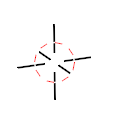
\includegraphics{Chapters/Images/Chapter_2/2_9_3DCursor.png}

\caption{\label{fig-2_9}3D-Cursor.}

\end{figure}%

\marginnote{3D-Cursor}

Innerhalb des 3D-Viewports ist ausserdem der 3D-Cursor sichtbar. Dieser
ist an einer bestimmten Position in der Szene platziert und dort mittels
eines rot-weissen Kreises dargestellt. Neu erstellte Objekte werden an
seiner Position in die Szene eingefügt und der 3D-Cursor kann als
Bezugspunkt für Transformationen verwendet werden.

\chapter{Navigation der Ansicht im
3D-Viewport}\label{navigation-der-ansicht-im-3d-viewport}

\marginnote{Navigation in der 3D-Ansicht}

Die Ansicht auf die Objekte im 3D-Viewport kann beliebig verändert
werden. Nebst der standardmässigen Ansichtssteuerung über die Maus kann
auch das Nummernfeld der Tastatur verwendet werden. In der Regel werden
beide Optionen verwendet. Die Navigation mit der Maus bietet tendenziell
eine grössere Flexibilität, während die Navigation mit der Tastatur eine
grössere Präzision ermöglicht.

\section{Navigation mit der Maus}\label{navigation-mit-der-maus}

\marginnote{Ansicht mit der Maus verändern}

Je nach Aufbau der verwendeten Computermaus unterscheidet sich die
Navigation durch den 3D-Viewport mit der Maus etwas. Bei einer
Computermaus mit einem Mausrad erfolgt die Navigation im 3D-Viewport
durch Mausbewegungen bei gedrückter Rad-Taste. Bei Trackpads oder Mäusen
mit integriertem Trackpad erfolgt die Navigation mittels
Wischbewegungen. Bei einer normalen Bewegung wird dabei lediglich die
Ansicht entsprechend der Bewegung rotiert. Durch gleichzeitiges Drücken
der \kbd{Shift}-Taste wird die Ansicht in die entsprechenden Richtungen
bewegt (ohne eine Rotation). Mittels gedrückter \kbd{Ctrl}-Taste kann
durch die Mausbewegung hinein- oder hinausgezoomt werden. Durch das
Drehen des Mausrads wird die Ansicht ebenfalls hinein- oder
hinausgezoomt.

\section{Navigation mit der Tastatur}\label{navigation-mit-der-tastatur}

\marginnote{Emulation des Nummernblocks}

Nebst der Maus kann auch die Tastatur verwendet werden, um die Ansicht
zu verändern. Diese Option ergibt sich allerdings nur, wenn man über
einen Nummernblock verfügt. Wenn kein Nummernblock zur Verfügung steht,
lassen sich auch die Zahlen-Tasten oberhalb der Buchstaben für die
Navigation verwenden. Hierfür muss allerdings in den
Benutzereinstellungen («\emph{Edit \textbar{} Preferences}») in den
Einstellungen zum «\emph{Input}» beim Keyboard-Reiter die Einstellung
«\emph{Emulate Numpad}» aktiviert werden.

\marginnote{Rotieren und Drehen der Ansicht}

Mittels der Tasten \kbd{2}, \kbd{4}, \kbd{6} und \kbd{8} kann die
Ansicht entsprechend ihrer relativen Anordnung auf dem Nummernblock
rotiert werden: Die Taste \kbd{2} rotiert nach unten, die Taste \kbd{4}
nach links, die Taste \kbd{6} nach rechts und die Taste \kbd{8} nach
oben. Werden dieselben Tasten bei gedrückter \kbd{Ctrl}-Taste gedrückt,
wird die Ansicht in die entsprechende Richtung bewegt, ohne eine
Rotation durchzuführen. Mittels gedrückter \kbd{Shift}-Taste kann die
Ansicht durch die Taste \kbd{6} zudem im Uhrzeigersinn und mittels der
Taste \kbd{4} gegen den Uhrzeigersinn gedreht werden. Um näher
hineinzuzoomen wird die Taste \kbd{+} und zum Hinauszoomen die Taste
\kbd{-} verwendet.

\marginnote{Präzise Ansichten ansteuern}

Mittels der Taste \kbd{1} kann die Ansicht direkt in die Vorderansicht
gedreht werden. Die Ansicht erfolgt anschliessend entlang der Y-Achse.
Die Rückansicht ist mit der Tastenkombination \kbd{Ctrl} + \kbd{1}
einstellbar. Mittels der Taste wird die Seitenansicht -- von der rechten
Seite aus zum Objekt hingewählt. Das Objekt wird in diesem Falle entlang
der X-Achse betrachtet. Mit der Tastenkombination \kbd{Ctrl} + \kbd{3}
ist die Seitenansicht von der linken Seite aus einstellbar. Um die Szene
aus der Vogelperspektive zu betrachten, kann die Taste \kbd{7} gedrückt
werden. Hierbei erfolgt die Ansicht der Z-Achse entlang. Mittels der
Tastenkombination \kbd{Ctrl} + \kbd{7} erfolgt die Ansicht von unten.

\marginnote{Perspektivische und orthogonale Darstelung}

Jede der Ansichten kann auf zwei Arten erfolgen: perspektivisch oder
orthogonal. Die perspektivische Ansicht berücksichtigt
Tiefeninformationen, sodass weiter entfernte Objekte kleiner dargestellt
werden. Die orthogonale Perspektive ignoriert die Tiefeninformationen,
wodurch weiter entfernte Objekte gleich gross angezeigt werden wie
nähere gleich grosse Objekte auf der entsprechenden Achse. Diese
Perspektive hat den Vorteil, dass Objekte in ihrer geometrischen Form in
2D betrachtet werden können. Mittels der Taste \kbd{5} kann zwischen
diesen beiden Ansichtsmodi gewechselt werden.

\marginnote{Kamera-Ansicht}

Mittels der Taste \kbd{0} kann die Ansicht direkt in die Position der
Kamera gelegt werden. Dadurch wird die Szene genau so betrachtet, wie
sie im finalen Render betrachtet werden wird. Wenn in einer Szene keine
Kamera vorhanden ist, steht diese Ansicht nicht zur Verfügung.Wenn
mehrere Kameras vorhanden sind, wird jeweils die Kamera, welche die
aktive Render Kamera darstellt, anvisiert. Um die Kameraperspektive zu
verlassen kann die Ansicht mittels der Maus bewegt werden, oder erneut
die Taste \kbd{0} gedrückt werden.

Merke\ldots{}

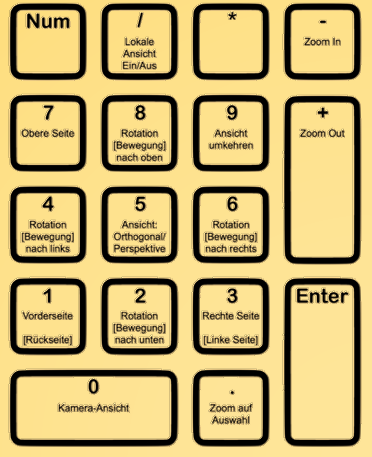
\includegraphics{Chapters/Images/Chapter_3/3_1_Number_Tabel.png}\hfill

\marginnote{Fokus auf ein Objekt}

In komplexeren Szenen kann es sein, dass man die Übersicht über die
Objekte verliert, oder dass sie sich gegenseitig im Weg stehen bei der
Ansicht. Mittels der Taste \kbd{.} auf dem Nummernblock wird die Ansicht
direkt auf ein ausgewähltes Objekt gezoomt. Diese Aktion lässt sich
nicht mit der Taste \kbd{.} ausserhalb des Nummernblocks emulieren.
Mittels der Taste \kbd{/} kann zudem die lokale Ansicht aktiviert
werden. In dieser Ansicht wird lediglich das ausgewählte Objekt
dargestellt, sodass es in komplexen Szenen besser betrachtet werden
kann. Allerdings muss anschliessend die Taste erneut gedrückt werden, um
die lokale Ansicht wieder zu verlassen. Auch diese Aktion lässt sich
nicht mit einer anderen Taste ausserhalb des Nummernblocks emulieren.

\section{Navigation mittels Gizmos}\label{navigation-mittels-gizmos}

Auf der rechten Seite des 3D-Viewports lassen sich zudem Schaltflächen
anzeigen, mit denen die Ansicht gesteuert werden kann. Um diese anzeigen
zu lassen, müssen die Gizmos eingeschaltet sein. Wird die linke
Maustaste auf das Kamera-Icon angewendet, wird die Kamera-Ansicht
aktiviert. Das Icon darunter, welches ein Gitternetz darstellt, dient
dem Wechsel zwischen perspektivischer und orthogonaler Ansicht. Die
beiden oberen Icons dienen dem Zoomen (mittels der Lupe) und dem Bewegen
der Ansicht (Hand). Hierfür muss das Icon angeklickt und die Maus
anschliessend bei weiterhin gedrückter Maustaste bewegt werden. Zuoberst
findet sich zudem ein Koordinatensystem, mit dem die Perspektive per
Mausklick oder mittels gedrückter Maustaste verändert werden kann.

\chapter{Erste Schritte}\label{erste-schritte}

\section{Die Default-Szene}\label{die-default-szene}

\marginnote{Objekte in der Default-Szene}

Beim Start eins neuen Projekts erscheint eine Default-Szene. Diese Szene
beinhaltet bereits die wesentlichen Dinge, welche für eine 3D-Szene
benötigt werden:

\begin{itemize}
\tightlist
\item
  \textbf{Würfel}: Genau in der Mitte der Szene befindet sich der
  Default-Cube. Bei diesem Würfel handelt es sich um ein 3D-Objekt. Er
  hat eine Grösse von 2x2x2 Metern.
\item
  \textbf{Kamera}: Von der Kamera aus wird eine Szene nach deren
  Verarbeitung (z.B. in einem geren derten Bild oder einem Video)
  betrachtet. In der Default-Szene ist die Kamera auf den Würfel
  gerichtet.
\item
  \textbf{Lichtquelle}: Die Lichtquelle wird dafür benötigt, dass der
  Würfel in der gerenderten Aufnahme beleuchtet wird. Ohne eine
  Lichtquelle sind die 3D-Objekte beim anschliessenden Rendern nicht
  sichtbar -- es sei denn, sie stellen selbst eine Lichtquelle dar.
\end{itemize}

\begin{tipp}{Weiterführende Informationen}
Die Default-Szene kann manuell angepasst werden. Hierfür muss zunächst eine Default-Szene erstellt werden, welche bei jedem Start erscheinen soll. Diese kann dann unter «*File* \| *Defaults* \| *Save Startup File*» als neue Start-up Szene gespeichert werden.
\end{tipp}

\section{Auswahl von Objekten}\label{auswahl-von-objekten}

\marginnote{Auswahl und Abwahl mittels Mausklick}

Durch das Anklicken mittels der linken Maustaste können Objekte im
3D-Viewport ausgewählt werden. Die ausgewählten Objekte sind
anschliessend anhand einer farblichen Markierung erkennbar. Durch das
Klicken in den leeren Raum des Viewport-Displays lassen sich die Objekte
wieder abwählen. Zudem wird durch die Auswahl eines anderen Objektes das
vorher ausgewählte Objekt abgewählt.

\marginnote{Mehrfachwahl mittels \kbd{Shift}}

Um mehrere Objekte gleichzeitig auszuwählen, gibt es verschiedene
Möglichkeiten. Eine Möglichkeit besteht darin, dass nacheinander Objekte
bei gedrückter \kbd{Shift}-Taste angeklickt und so zur Auswahl
hinzugefügt werden. Durch die Auswahl von mehreren Objekten wird das
zuletzt ausgewählt Objekt mit einer orangen und die vorherig
ausgewählten Objekte mittels einer roten Farbe markiert.

\marginnote{Aktives Objekt}

Die Markierung mit einer orangen Farbe gibt jeweils an, dass es sich bei
diesem Objekt um das aktive Objekt handelt. Diese Unterscheidung wird in
späteren Kapiteln noch von Bedeutung sein, etwa wenn Merkmale vom
aktiven Objekt auf andere Objekte übertragen werden sollen, oder wenn
ein Objekt in Bezug zum aktiven Objekt verändert werden soll. Für den
aktuellen Stand ist jedoch vor allem wichtig, wie die Objekte ausgewählt
werden, und hierfür macht die rote oder orange Markierung noch keinen
Unterschied aus.

\marginnote{Box-Selection mittels \kbd{B}}

Alternativ kann auf den Box-Select-Modus zurückgegriffen werden. Dieser
wird mit der \kbd{B} Taste aktiviert. Durch das Gedrückthalten der
linken Maustaste lässt sich anschliessend ein Viereck über den
Bildschirm ziehen. Alle Objekte, welche sich anschliessend innerhalb
dieser Box befinden, werden nach dem Loslassen der linken Maustaste
ausgewählt. Mittels der Taste \kbd{esc} oder der rechten Maustaste lässt
sich die Box-Selection abbrechen.

\marginnote{Circle-Selection mittels \kbd{C}}

Alternativ können Objekte auch mit dem Circle-Select-Modus ausgewählt
werden. Der Circle-Select Modus wird mit der Taste \kbd{C} aktiviert.
Bei der Verwendung des Circle-Select-Modus ist der Mauszeiger von einem
Kreis umgeben. Mithilfe des Mausrads kann die Grösse des Kreises
eingestellt werden. Durch einen Klick mit der linken Maustaste werden
die Objekte, welche sich innerhalb dieses Kreises befinden, alle
ausgewählt. Durch das Bewegen des Mauszeigers bei gedrückter linken
Maustaste können so eine Reihe weiterer Objekte ausgewählt werden. Der
Circle-Select-Modus muss allerdings aktiv beendet werden, da ein
weiterer Klick mit der linken Maustaste zu einer weiteren Auswahl von
Objekten führt. Um den Circle-Select-Modus wieder zu verlassen, kann die
Taste \kbd{Enter}, \kbd{esc} oder der rechten Maustaste gedrückt werden.
Anschliessend sind alle Objekte, welche im Circle-Select-Modus
angeklickt wurden, ausgewählt.

\marginnote{Auswahl umkehren}

Mittels der Tastenkombination \kbd{Ctrl} + \kbd{I} ist es möglich, die
Auswahl umzukehren. Dadurch werden alle ausgewählten Objekte abgewählt
und alle anderen Objekte ausgewählt. Wenn alle Objekte innerhalb einer
Szene ausgewählt werden sollen, kann die Taste \kbd{A} gedrückt werden.
Dadurch werden auch Objekte, die möglicherweise ausserhalb des gerade
sichtbaren Bereichs liegen, ausgewählt.

\marginnote{Auswahl von Objekten im Outliner}

Im Outliner auf der rechten Seite wird mittels einer blauen Markierung
angezeigt, welches Objekt gerade ausgewählt ist. Zudem lassen sich auch
hier Objekte auswählen, indem sie mittels der linken Maustaste
angeklickt werden. Die Auswahl von mehreren Objekten kann analog wie im
Viewport-Display mittels des Gedrückthaltens der \kbd{Shift}-Taste
getroffen werden oder durch eine Box-Auswahl mittels der Taste \kbd{B} .
Auch hier können alle Objekte mittels der Taste \kbd{A} gemeinsam
ausgewählt werden. Der Circle-Select-Modus funktioniert allerdings nicht
im Outliner.

\section{Hinzufügen von Objekten}\label{hinzufuxfcgen-von-objekten}

\marginnote{Hinzufügen von Objekten mittels \kbd{Shift} + \kbd{A}}

Mittels der Tastenkombination \kbd{Shift} + \kbd{A} erscheint beim
Mauszeiger das Menü-Feld «\emph{Add}». Dabei handelt es sich um dasselbe
Menü-Feld, welches auch unter dem Reiter «\emph{Add}» in der linken
oberen Ecke aufgerufen werden kann. Mithilfe dieses Menü-Felds können
eine Reihe von verschiedenen Objekten im Viewport Display hinzugefügt
werden. Es gibt eine Reihe verschiedener Objektarten, welche hinzugefügt
werden können. Beispielsweise kann unter «\emph{Mesh} \textbar{}
\emph{Cube}» ein Würfel in die Szene hinzugefügt werden. Ein neues
Objekt wird jeweils an der Position des 3D-Cursors eingefügt.

\marginnote{Neue Objekte anpassen}

Wenn ein neues Objekt hinzugefügt wird, wird dieses Objekt direkt
angewählt und farblich markiert. Zudem erscheint in der unteren linken
Ecke des Viewport-Displays ein Kontext-Menü-Feld. Dieses Menü-Feld kann
aufgeklappt werden und beinhaltet Einstellungen zum Objekt, welche noch
spezifiziert werden können. Beim Hinzufügen eines Würfels besteht etwa
die Möglichkeit, dass man dessen Grösse (Size), seine Position und seine
Rotation entlang der X-, Y- und Z-Achse anpassen kann. Da das Objekt
jeweils an der Stelle des 3D-Cursors erscheint, entspricht die Position
des Objektes in diesem Menü jeweils auch der Position des 3D-Cursors.

\marginnote{Kontext-Menü zum neuen Objekt}

Das Kontext-Menü, welches beim Hinzufügen von Objekten erscheint, ist
nur temporär vorhanden. Sobald mit der linken Maustaste in einen Bereich
ausserhalb des Kontext-Menüs geklickt wird, verschwindet das Menü-Feld.
Es gibt keine Möglichkeit, dieses Menü-Feld zurückzuholen -- es ist für
immer für dieses Objekt verschwunden. Wenn das Menü nochmals benötigt
werden sollte, muss das entsprechende Objekt erneut zur Szene
hinzugefügt werden.

Merke\ldots{}

Kontext-Menü-Felder erscheinen in der linken unteren Ecke des
Viewport-Displays und sind nur temporär verfügbar. Nach einem Klick
ausserhalb des Menü-Feldes verschwinden dieses Felder und können nicht
mehr zurückgeholt werden.

\section{Löschen von Objekten}\label{luxf6schen-von-objekten}

\marginnote{Löschen von Objekten mittels \kbd{X}}

Wenn ein Objekt gelöscht werden soll, muss dieses zunächst ausgewählt
werden. Mittels der Taste \kbd{X} wird der Befehl für die Löschung des
ausgewählten Objektes gegeben. Dieser muss anschliessend bestätigt
werden, entweder mit einem Mausklick auf das daraufhin beim Mauszeiger
erscheinende «\emph{Delete}»-Feld oder mittels der Taste \kbd{Enter}.
Alternativ kann auch die Taste \kbd{Delete} verwendet werden -- hierbei
wird das Objekt direkt gelöscht, ohne dass eine Bestätigung nötig ist.

Übung 2: Hinzufügen und Löschen

\textbf{Übung 2.1}

Löschen Sie alle Objekte aus der Szene.

\textbf{Übung 2.2}

Erstellen Sie einen neuen Würfel mit der Grösse 1 und einer Rotation von
90°. Welche Achse Sie hierfür wählen, spielt keine Rolle.

Merke\ldots{}

Mittels \kbd{Shift} + \kbd{A} erscheint beim Mauszeiger das Menü zum
Hinzufügen von Objekten.

Um Objekte zu löschen, müssen sie zunächst ausgewählt werden und können
anschliessend mit der Taste \kbd{X} oder \kbd{Delete} gelöscht werden.

\section{Objekte vervielfältigen}\label{objekte-vervielfuxe4ltigen}

\marginnote{Methoden zur Vervielfältigung von Objekten}

Ausgewählte Objekte können auf verschiedene Arten dupliziert werden.
Jede diese Arten hat ihre eigenen Besonderheiten:

\begin{itemize}
\tightlist
\item
  Duplizieren des Objektes
\item
  Verbundene Duplikate erstellen
\item
  Einfügen einer Kopie des Objektes mittels Copy-Paste
\end{itemize}

\subsection{Objekte duplizieren}\label{objekte-duplizieren}

\marginnote{Duplikat eines Objektes erstellen mittels \kbd{Shift} + \kbd{D}}

Die schnellste Methode, um Objekte zu duplizieren, besteht darin, dass
die entsprechenden Objekte, welche dupliziert werden sollen, ausgewählt
werden und anschliessend mit der Tastenkombination \kbd{Shift} + \kbd{D}
der Befehl zur Duplikation der Objekte gegeben wird. Dadurch entsteht an
der Position des originalen Objekts ein Duplikat, welches mit der
Bewegung des Mauszeigers im Raum bewegt werden kann. Durch einen Klick
mit der linken Maustaste, \kbd{Space}- oder \kbd{Enter}-Taste wird das
Objekt anschliessend platziert. Die Bewegung des duplizierten Objekts
kann auch mittels abgebrochen werden. Dadurch wird das Duplikat
allerdings nicht gelöscht, sondern an derselben Position wie das
Original platziert.

\subsection{Verbundene Duplikate
erstellen}\label{verbundene-duplikate-erstellen}

\marginnote{Verbundene Duplikate erstellen mittels \kbd{Alt} + \kbd{D}}

Nebst einem normalen Duplikat kann auch ein verbundenes Duplikat
erstellt werden. Hierfür wird nach der Auswahl der zu duplizierenden
Objekte die Tastenkombination \kbd{Alt} + \kbd{D} gedrückt. Auch bei
dieser Methode kann das Objekt mit der Maus im Raum bewegt und mittels
der linken Maustaste oder \kbd{Enter}Taste platziert werden. Wird nun in
weiteren Arbeitsschritten entweder das originale oder das verbunden
duplizierte Objekt bearbeitet, führt dies dazu, dass dieselben
Veränderungen gleichzeitig auch bei allen verbundenen Objekten
durchgeführt werden.

\subsection{Copy-Paste von Objekten}\label{copy-paste-von-objekten}

\marginnote{Objekte mittels Copy-Paste vervielfältigen}

Eine weitere Methode zur Vervielfältigung von Objekten besteht darin,
dass die zu vervielfältigenden Objekte ausgewählt und mittels \kbd{Ctrl}
+ \kbd{C} kopiert und anschliessend mittels \kbd{Ctrl} + \kbd{V} wieder
eingefügt werden. Im Gegensatz zur normalen und zur verbundenen
Duplizierung werden die eingefügten Objekte direkt platziert und müssen
durch weitere Befehle verschoben werden. Zudem werden bei dieser Methode
auch von den Materialien des Objektes eine Kopie erstellt, welche dann
dem neu eingefügten Objekt zugewiesen wird. Dadurch führt eine
Bearbeitung des Materials des originalen Objekts nicht zu einer
Veränderung des Materials des neu eingefügten Objekts. Allerdings kann
dem eingefügten Objekt auch wieder das originale Material zugewiesen
werden.

\section{Verbinden von Objekten}\label{verbinden-von-objekten}

\marginnote{Join mittels \kbd{Ctrl} + \kbd{J}}

Mehrere Objekte lassen sich auch verbinden, sodass sie zu einem Objekt
werden. Hierfür müssen die zu verbindenden Objekte markiert werden. Die
Verbindung der Objekte erfolgt anschliessend mittels der
Tastenkombination \kbd{Ctrl} + \kbd{J} . Wichtig ist dabei, dass eines
der markierten Objekte das aktive Objekt darstellt. Üblicherweise
handelt es sich dabei um das zuletzt ausgewählte Objekt. Das aktive
Objekt ist jeweils anhand einer orangen statt einer roten Markierung
ersichtlich. Die anderen Objekte werden anschliessend zum aktiven Objekt
hinzugefügt. Wenn mehrere Objekte ausgewählt sind, allerdings kein
Objekt der Auswahl das aktive Objekt darstellt, wird das Verbinden von
Objekten nicht durchgeführt.

\section{Verstecken von Objekten}\label{verstecken-von-objekten}

\marginnote{Verstecken von Objekten mittels \kbd{H}}

Gerade bei sehr komplexen Szenen kann es vorkommen, dass sich die
Objekte gegenseitig verdecken und die Bearbeitung etwas schwieriger
wird. In diesem Falle gibt es die Möglichkeit, Objekte in der Ansicht zu
verstecken. Ausgewählte Objekte können mittels der Taste versteckt
werden. Im Outliner sind die Objekte nach wie vor noch angegeben,
allerdings grau hinterlegt. Mittels der Tastenkombination \kbd{Alt} +
\kbd{H} werden alle versteckten Objekte wieder angezeigt. Mittels der
Tastenkombination \kbd{Shift} + \kbd{H} lassen sich zudem alle Objekte,
ausser den ausgewählten Objekten, verstecken. Dadurch sind nur noch die
markierten Objekte sichtbar.

\begin{tipp}{Weiterführende Informationen}
Statt Objekte in einer Szene zu verstecken kann alternativ auch die lokale Ansicht mittels der Taste \kbd{/} auf diese Objekte angewendet werden. In dieser Ansicht werden alle anderen Objekte ausgeblendet. Um wieder in die normale Ansicht zu gelangen, muss erneut die Taste \kbd{/} gedrückt werden.
\end{tipp}

\marginnote{Versteckte Objekte im Outliner aufdecken}

Um einzelne Objekte wieder anzeigen zu lassen, kann im Outliner das
geschlossene Auge neben dem entsprechenden Objekt angewählt werden.
Analog kann auch ein geöffnetes Auge angewählt werden, um die Objekte zu
verstecken. Das Verstecken von Objekten bezieht sich nur auf den
Viewport-Display. In einem finalen Render werden die Objekte trotzdem
gerendert und sind dementsprechend sichtbar.

\section{Anordnen in Collections}\label{anordnen-in-collections}

\marginnote{Collections}

Im Outliner lassen sich die verschiedenen Objekte in Collections
anordnen. Hierfür werden die Objekte jeweils in eine Collection
hineingezogen. Anschliessend werden die Objekte innerhalb dieser
Collection aufgelistet. Auch andere Collections können in eine
Collection hineingezogen werden. Somit können mithilfe der Collections
Ordnerstrukturen im Outliner erstellt werden. Dies ermöglicht, dass die
Objekte innerhalb einer Collection als gemeinsame Gruppe für komplexere
Vorhaben verwendet werden können -- etwa für Partikel-Effekte.

\marginnote{Hinzufügen und Deaktivieren von Collections}

Mithilfe der Schaltfläche oben rechts in der Ecke des Outliners können
neue Collections hinzugefügt werden. Hierfür muss je nach
Bildschirmgrösse allenfalls der Header des Outliners nach rechts
gescrollt oder der Outliner vergrössert werden. Mittelt dem
Kontrollkästchen neben einer Collection lassen sich die Objekte
innerhalb einer Collection deaktivieren. Die entsprechenden Objekte
werden anschliessend im Viewport nicht mehr angezeigt und auch beim
Rendern nicht mehr berücksichtig.

\section{Speichern}\label{speichern}

\marginnote{Zwischenspeichern mittels \kbd{Ctrl} + \kbd{S} ist unabdingbar}

Bisher wurden bereits einige Tastenkombinationen angesprochen. Die
wichtigste Tastenkombination stellt allerdings die Kombination für das
Abspeichern des aktuellen Projekts dar: \kbd{Ctrl} + \kbd{S}.
Zwischenspeichern ist bei der Arbeit mit Blender eine wichtige
Empfehlung. Je nach Komplexität des Projektes kann es manchmal
vorkommen, dass das Programm unerwartet abstürzt und die Fortschritte
bis zum letzten Speicherpunkt verloren gehen. Aus diesem Grund empfiehlt
es sich, das Projekt lieber einmal zu viel als einmal zu wenig
abzuspeichern.

\marginnote{Kopie speichern}

Alternativ kann das Projekt auch unter «\emph{File} \textbar{}
\emph{Save}» abgespeichert werden. Nebst der Möglichkeit, dass ein
Projekt unter einem neuen Namen gespeichert und fortgeführt wird
(«\emph{File} \textbar{} \emph{Save} as» bzw. \kbd{Ctrl} + \kbd{Shift} +
\kbd{S}), gibt es auch die Möglichkeit, mittels «\emph{File} \textbar{}
\emph{Save Copy}» (\kbd{Ctrl} + \kbd{Alt} + \kbd{S}) eine Backup-Version
abzuspeichern und in dem originalen File weiterzuarbeiten.

\marginnote{.blend-Files}

Die Projekte werden jeweils in Blenders programmeigenem Format
«\emph{.blend}» abgespeichert. Diese Datei enthält alle Objekte,
Animationen und Einstellungen des Projektes. Das .blend-Dateiformat kann
lediglich mit Blender geöffnet werden. Wenn externe Dateien
(beispielsweise Texturen, Soundeffekte oder Videos) im Projekt
eingebunden werden, müssen diese ebenfalls mit dem Projekt weitergegeben
werden. Es gibt jedoch die Möglichkeit, unter «\emph{File} \textbar{}
\emph{External Data} \textbar{} \emph{Pack all into.blend}» alle diese
externen Dateien in das .blend-File einzuspeichern. Dadurch erhöht sich
allerdings die Grösse des abgespeicherten Files.

\marginnote{Exportieren}

Um Programme auch für andere Projekte verfügbar zu machen, müssen sie in
einem anderen Dateiformat ausgegeben werden. Unter «\emph{File}
\textbar{} \emph{Export}» steht eine Reihe von verschiedenen
Dateiformaten zur Verfügung, welche von unterschiedlichen Programmen
geöffnet werden können. Die meisten dieser Dateiformate kann Blender
wiederum importieren und darstellen.

Merke\ldots{}

Lieber einmal mehr mit der Kombination \kbd{Ctrl} + \kbd{S}, speichern,
als die Fortschritte zu verlieren.

\chapter{Objektarten}\label{objektarten}

\marginnote{Verschiedene Arten von Objekten}

Beim Hinzufügen von Objekten mittels der Tastenkombination \kbd{Shift} +
\kbd{A} erscheint das Menü für das Hinzufügen von Objekten beim
Mauszeiger. Die verschiedenen Objekte sind dabei in verschiedene Typen
von Objekten unterteilt. Diese Objekte unterscheiden sich hinsichtlich
ihres Aufbaus, aber auch hinsichtlich ihrer Funktion.

\section{Mesh}\label{mesh}

\marginnote{Meshes}

Ein Mesh stellt ein 3D-Objekt dar. Meshes haben eine gitterähnliche
Struktur aus Punkten, Linien und verbundenen Flächen, welche in ihrer
Gesamtstruktur das Objekt darstellen. Der Hauptfokus dieses Kurses wird
auf die Meshes gelegt, von daher werden sie später noch ausführlich
beschrieben.

\section{Curve}\label{curve}

\marginnote{Kurven}

Vor der Entwicklung der Meshes wurden in Computergrafiken Kurven und
Oberflächen verwendet. Sie haben den Vorteil, dass sie weniger
Computerleistung benötigen. Kurven verfügen über weniger Kontrollpunkte,
wodurch sie auch einfacher zu bearbeiten sind. In einigen Anwendungen
werden sie heute immer noch verwendet. Blender verfügt über zwei Arten
von Kurven: Bézier-Kurven und Nurbs-Kurven. Die beiden Arten von Kurven
unterscheiden sich hinsichtlich ihrer zugrundeliegenden Berechnungen.

\marginnote{Kurven können Oberflächen enthalten}

Neu hinzugefügte Kurven beinhalten zunächst keine Oberfläche und
erscheinen dadurch nicht beim Rendern. Allerdings können ihnen
Oberflächen hinzugefügt werden, sodass sie auch als Objekte erkennbar
werden. Zudem können Kurven auch als Hilfestellung bei Animationen
verwendet werden, indem etwa Pfade für eine Animation mit ihnen
vorgegeben werden.

\section{Surface}\label{surface}

\marginnote{Surfaces}

Die Surfaces sind ähnlich zu den Kurven. Während Kurven 2D-Objekte
darstellen, sind die Surfaces ihre 3D-Erweiterungen. Obwohl Kurven und
Surfaces somit denselben Typ von Objekten darstellen, können sie nicht
gleichzeitig auftreten. In einem Objekt können somit nicht sowohl Kurven
als auch Surfaces vorhanden sein.

\section{Metaball}\label{metaball}

\marginnote{Metas}

Metabälle gehören zur Objekt-Familie der Metas, welche Blender
prozedural aufbaut. Anders als beispielsweise Meshes oder Kurven sind
sie nicht durch Kontrollpunkte oder Gitternetze aufgebaut, sondern
werden mathematisch von Blender berechnet. Wenn zwei Meta-Objekte in der
Nähe voneinander sind, können sie miteinander interagieren.

\section{Text}\label{text}

\marginnote{Text}

Text-Objekte beinhalten einen Text, der anschliessend als Objekt
dargestellt wird. Der Text hat dabei wie die Kurven oder die Oberflächen
lediglich zwei Dimensionen.

\section{Volume}\label{volume}

\marginnote{Volumen-Objekte}

Volumen-Objekte sind lediglich Objekt-Container. Ihnen können
OpenVDB-Dateien angehängt werden, um volumetrische Daten (beispielsweise
Wolken oder Rauch) zu erzeugen. Diese Dateien können mithilfe von
Blenders eigenen Simulationen erzeugt werden, oder in anderen Programmen
erzeugt und abgespeichert werden.

\section{Grease Pencil}\label{grease-pencil}

\marginnote{Grease Pencil}

Grease Pencils sind Objekte, welche es ermöglichen, direkt in den
dreidimensionalen Raum zu zeichnen. Zudem können mit ihnen
2D-Animationen erstellt werden -- etwa wenn Blender für ein 2D- statt
3D-Projekt verwendet wird. Objekte der Kategorie «Grease Pencil» sind
dabei eigentlich Behälter-Objekte, in welche anschliessend die Linien
gezeichnet werden.

\section{Armature}\label{armature}

\marginnote{Armaturen}

Armaturen werden verwendet, um Meshes zu animieren. Hierbei wird
innerhalb eines Meshes ein Gerüst erstellt, anhand dessen die Animation
anschliessend erfolgen soll. Dieses Gerüst stellt sozusagen das Skelett
dar, welches anschliessend für die Animation verwendet werden soll.
Dementsprechend werden die einzelnen Gerüstteile auch Bones (Knochen)
genannt. Armaturen werden beim Rendern nicht angezeigt. Bei ihnen
handelt es sich lediglich um ein Werkzeug zur Animation.

\section{Lattice}\label{lattice}

\marginnote{Lattice}

Das Lattice stellt ein dreidimensionales Gerüst aus Punkten dar, welches
allerdings nicht gerendert werden kann. Es dient als Werkzeug zur
komplexeren Transformation von Objekten.

\section{Empty}\label{empty}

\marginnote{Empties}

Empties sind Knotenpunkte an einem einzigen Punkt in der virtuellen
Welt. Sie beinhalten weder Oberflächen noch Volumen und können auch
nicht gerendert werden. Sie lassen sich allerdings beispielsweise als
Bezugspunkte für Objekte verwenden.

\section{Image}\label{image}

\marginnote{Bilder}

Blender ermöglichet es, dass auch externe Bilddateien direkt einer Szene
hinzugefügt werden können. Hierfür kann ein solches Image-Objekt
erstellt und das Bild anschliessend diesem Objekt angefügt werden.
Bilder können allerdings auch direkt in den Viewport-Display gezogen
werden, wodurch sie anschliessend hinzugefügt werden.

\section{Light}\label{light}

\marginnote{Lichtquellen}

Licht-Objekte stellen die Quelle für die Beleuchtung von Szenen dar. Sie
sind nicht als Mesh oder Kurve modellierbar, sondern stellen vielmehr
einen Punkt oder Bereich dar, von dem die Beleuchtung ausgeht.

\section{Light-Probe}\label{light-probe}

\marginnote{Light Probes}

Light Probes werden in der Eevee-Render-Engine als Hilfsobjekte
verwendet. Dabei werden beispielsweise Informationen über indirekte
Beleuchtungseffekte gespeichert. Diese Informationen werden
anschliessend im finalen Render berücksichtigt, während das
Light-Probe-Objekt als solches nicht im finalen Render dargestellt wird.

\section{Camera}\label{camera}

\marginnote{Kamera}

Kameras stellen den Punkt dar, von dem aus die Welt in der gerenderten
Szene betrachtet wird. Die Kameras als solche sind in den gerenderten
Bildern nicht sichtbar.

\section{Speaker}\label{speaker}

\marginnote{Lautsprecher}

Speaker werden verwendet, um an bestimmten Positionen in der Szene Töne
erklingen zu lassen. So wie die Lichtquellen sind die Speaker nicht
modellierbar, sondern stellen einen Punkt in der drei dimensionalen Welt
dar, von dessen Position ein Klang ausgeht.

\section{Force Field}\label{force-field}

\marginnote{Kraftfelder}

Force Fields sind Objekte, welche in Simulationen Kräfte auf andere
Objekte ausüben können. So können andere Objekte beispielsweise
angezogen oder absorbiert werden. Beim Rendern sind diese Objekte als
solche nicht sichtbar, allerdings die Auswirkungen, welche deren Kräfte
auf Objekte haben können.

\section{Collection Instance}\label{collection-instance}

\marginnote{Collections}

Collections sind Einheiten, um Objekte anzuordnen und zu gruppieren. Sie
erscheinen nicht im Viewport, sind aber im Outliner aufzufinden. Sie
können wie Dateiordner verstanden werden.

\section{Zusammenfassung der
Objektarten}\label{zusammenfassung-der-objektarten}

\marginnote{Verschiedene Objektarten}

Die verschiedenen Objektarten dienen also entweder der Darstellung von
Objekten, der Darstellung von externen Dateien, der Darstellung der
Szene oder haben vor allem unterstützende Funktionen:

\begin{longtable}[]{@{}
  >{\raggedright\arraybackslash}p{(\columnwidth - 12\tabcolsep) * \real{0.1429}}
  >{\raggedright\arraybackslash}p{(\columnwidth - 12\tabcolsep) * \real{0.1429}}
  >{\raggedright\arraybackslash}p{(\columnwidth - 12\tabcolsep) * \real{0.1429}}
  >{\raggedright\arraybackslash}p{(\columnwidth - 12\tabcolsep) * \real{0.1429}}
  >{\raggedright\arraybackslash}p{(\columnwidth - 12\tabcolsep) * \real{0.1429}}
  >{\raggedright\arraybackslash}p{(\columnwidth - 12\tabcolsep) * \real{0.1429}}
  >{\raggedright\arraybackslash}p{(\columnwidth - 12\tabcolsep) * \real{0.1429}}@{}}
\caption{Übersicht über die verschiedenen Objektarten. Mit einem Stern
markierten Objektarten sind renderbare Objekte.}\tabularnewline
\toprule\noalign{}
\begin{minipage}[b]{\linewidth}\raggedright
Gitter-basiert*
\end{minipage} & \begin{minipage}[b]{\linewidth}\raggedright
Kurven-basiert*
\end{minipage} & \begin{minipage}[b]{\linewidth}\raggedright
\textbf{Metas}*
\end{minipage} & \begin{minipage}[b]{\linewidth}\raggedright
Linien*
\end{minipage} & \begin{minipage}[b]{\linewidth}\raggedright
Szenen-Tools
\end{minipage} & \begin{minipage}[b]{\linewidth}\raggedright
Externe Daten
\end{minipage} & \begin{minipage}[b]{\linewidth}\raggedright
Hilfs-Werkzeuge
\end{minipage} \\
\midrule\noalign{}
\endfirsthead
\toprule\noalign{}
\begin{minipage}[b]{\linewidth}\raggedright
Gitter-basiert*
\end{minipage} & \begin{minipage}[b]{\linewidth}\raggedright
Kurven-basiert*
\end{minipage} & \begin{minipage}[b]{\linewidth}\raggedright
\textbf{Metas}*
\end{minipage} & \begin{minipage}[b]{\linewidth}\raggedright
Linien*
\end{minipage} & \begin{minipage}[b]{\linewidth}\raggedright
Szenen-Tools
\end{minipage} & \begin{minipage}[b]{\linewidth}\raggedright
Externe Daten
\end{minipage} & \begin{minipage}[b]{\linewidth}\raggedright
Hilfs-Werkzeuge
\end{minipage} \\
\midrule\noalign{}
\endhead
\bottomrule\noalign{}
\endlastfoot
Mesh & Curve & Metaball & Grease Pencil & Camera & Volume & Armature \\
& Surface & & & Light & Image & Lattice \\
& Text & & & Speaker & & Empty \\
& & & & & & Force Field \\
& & & & & & Speaker \\
& & & & & & Light Probe \\
& & & & & & Collection Instance \\
\end{longtable}

\chapter{Primitive Meshes}\label{primitive-meshes}

\marginnote{Primitives}

Wie bereits erwähnt fokussiert sich dieser Kurs auf den Umgang mit
Meshes. In der Auswahl zum Hinzufügen werden verschiedene grundlegende
Formen von Meshes bereitgestellt. Diese grundlegenden Formen werden als
Primitives bezeichnet. Zu den Primitives gehören:

\begin{itemize}
\tightlist
\item
  Plane
\item
  Cube
\item
  Circle
\item
  UV Sphere
\item
  Ico Sphere
\item
  Cylinder
\item
  Cone
\item
  Torus
\item
  Grid
\item
  Monkey
\end{itemize}

\section{Plane}\label{plane}

\marginnote{Fläche}

Die Plane stellt das grundlegendste Primitive dar. Es handelt sich dabei
lediglich um eine einzelne Fläche, bestehend aus einer Fläche mit vier
Eckpunkten. Per Default hat die Plane eine Dimensionalität von 2x2x0
Metern.

\section{Cube}\label{cube}

\marginnote{Würfel}

Der Cube entspricht dem Standardwürfel, den Blender bei der
Default-Szene anzeigt. Per Default hat der Würfel eine Dimensionalität
von 2x2x2 Metern.

\section{Circle}\label{circle}

\marginnote{Kreis}

Der Circle entspricht einem runden Kreis mit dem Radius von einem Meter,
wodurch er eine Dimensionalität von 2x2x2 Metern innehat. Der Kreis
besteht lediglich aus mit Linien verbundenen Punkten, ohne eine innere
Fläche. Allerdings kann im Kontext-Menü zum Hinzufügen des Kreises auch
eine Füllfläche erstellt werden.

\section{UV Sphere}\label{uv-sphere}

\marginnote{Kugel bestehend aus Vierecken}

Die UV-Sphere stellt eine Kugel dar, mit der Dimensionalität von 2x2x2
Metern. Die Kugel besteht aus viereckigen Flächen, wobei sie an den
Endpunkten der Z-Achse durch dreieckige Flächen verbunden ist. Die
Anzahl der Segmente um die Kugel herum sowie die Anzahl Ringe lassen
sich im Kontext-Menü beim Erstellen der Kugel einstellen. Die Segmente
beschreiben dabei die Anzahl Unterteilungen, welche ein Ring entlang der
XY-Achse der Kugel beinhaltet, während die Anzahl Ringe beschreibt, wie
oft die Kugel der Z-Achse entlang unterteilt werden soll.

\section{Ico Sphere}\label{ico-sphere}

\marginnote{Kugel bestehend aus Dreiecken}

Die Ico-Sphere stellt ebenfalls eine Kugel dar, allerdings mit den
Dimensionen 1.9x2x2 Meter. Anders als die UV-Sphere besteht sie nur aus
dreieckigen Flächen. Dies hat den Vorteil, dass die Form der Faces über
die ganze Kugel hinweg etwa gleich bleibt. Im Kontext-Menü zur
Erstellung der Ico Sphere kann mit der Anzahl Subdivisions eingestellt
werden, wie oft die Dreiecke dieser Kugel unterteilt werden sollen. Mit
zunehmenden Subdivisions nähert sich die X-Dimensionalität auch 2 Metern
an.

\section{Cylinder}\label{cylinder}

\marginnote{Zylinder}

Der Zylinder stellt zwei Kreise dar, welche durch Flächen miteinander
verbunden sind. Seine Dimensionalität entspricht 2x2x2 Metern mit einem
Radius der Kreise von 1 Meter. Im Kontext-Menü zur Erstellung des
Zylinders lässt sich die Anzahl Unterteilungen im Kreis einstellen.
Zudem lässt sich hier analog zum Kreis einstellen, ob die Kreisfläche
mit einer Füllfläche versehen werden soll und mit welcher Art von
Füllfläche.

\section{Cone}\label{cone}

\marginnote{Kegel}

Der Kegel stellt einen Spezialfall des Zylinders dar, bei dem die Radien
der beiden Enden variiert werden können und einer der beiden Kreise
einen Radius von 0 innehat. Auch hier kann wieder eingestellt werden,
wie viele Unterteilungen die Kreise innehaben sollen und wie die
Kreisflächen gestaltet werden sollen.

\section{Torus}\label{torus}

\marginnote{Torus}

Der Torus stellt eine ringförmige Gestalt dar, welche aus einer Major-
und einer Minor-Komponente besteht. Die Major-Komponente beschreibt
dabei den Kreis von der Vogelperspektive herab auf den Torus und die
Minor-Komponente den Kreis, welcher sich aus dem Querschnitt des Torus
ergibt. Für beide Komponenten kann die Anzahl Unterteilungen über das
Segment-Feld im Kontext-Menü eingegeben werden. Die Dimensionalität kann
entweder hinsichtlich der Major- und Minor-Komponente festgelegt werden
oder alternativ als Radius des inneren und des äusseren Ringes.

\begin{figure}

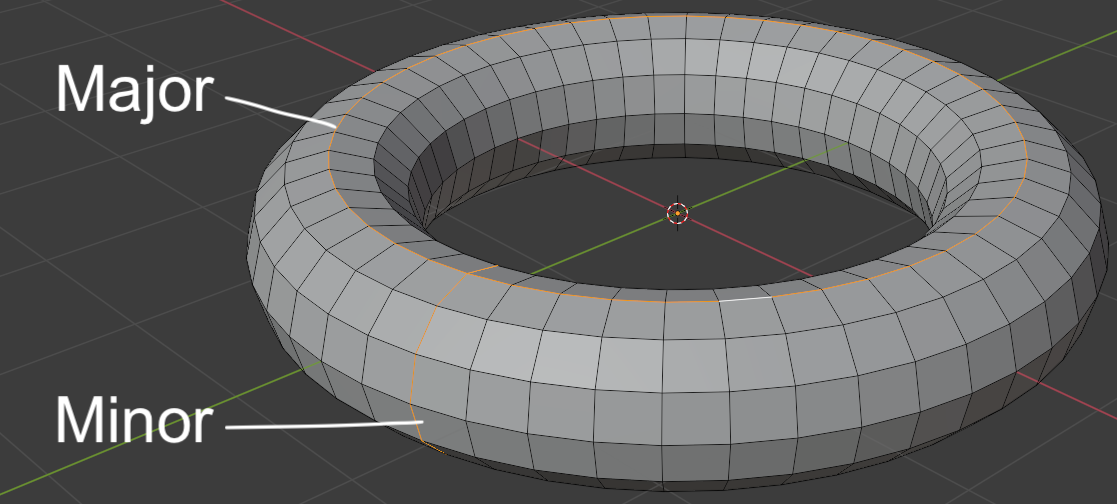
\includegraphics{Chapters/Images/Chapter_6/6_1_Major_Minor_Components_Torus.png}

\caption{\label{fig-1_1}Major- und Minor-Komponente des Torus.}

\end{figure}%

\section{Grid}\label{grid}

\marginnote{Gitternetz}

Das Grid stellt eine Alternative zur glatten Fläche dar, ist allerdings
bereits in weitere kleine viereckige Flächen unterteilt. Im Kontext-Menü
lässt sich anhand der Subdivisions eingeben, wie viele Unterteilungen
das Gitternetz entlang der X- und der Y-Achse haben soll. Die
Dimensionalität des Grids ist analog zur Plane per Default 2x2x0 Meter.

\section{Monkey}\label{monkey}

\marginnote{Suzanne}

Bei der Auswahl des Monkeys generiert Blender das Modell eines
Affenkopfs. Dabei handelt es sich um Suzanne, das Maskottchen von
Blender.

\chapter{Methoden der
Objekt-Transformation}\label{methoden-der-objekt-transformation}

\section{Die drei grundlegenden
Objekt-Transformationen}\label{die-drei-grundlegenden-objekt-transformationen}

\marginnote{Grundlegende Transformationen}

Jegliche 3D-Meshes beinhalten drei grundlegende Eigenschaften. Diese
Grundeigenschaften können jederzeit variiert werden. Es handelt sich
dabei um:

\begin{itemize}
\tightlist
\item
  Position
\item
  Rotation
\item
  Skalierung
\end{itemize}

Alle drei Optionen sind in der Sidebar (ein /ausblenden mittels \kbd{N})
unter dem Menü «\emph{Item}» unter dem Reiter «\emph{Transform}»
sichtbar. Die Eigenschaften beziehen sich jeweils auf das ausgewählte
Objekt. Wenn kein Objekt ausgewählt ist, beziehen sie sich auf das
zuletzt ausgewählte Objekt. Mittels der Einstellungen in der Sidebar
lassen sich diese drei Eigenschaften beliebig durch die Eingabe von
Zahlen variieren.

\begin{tipp}{Weiterführende Informationen}
Statt Zahlen können auch mathematische Berechnungen in die Felder eingegeben werden. Dadurch lassen sich komplexere Positionen ermitteln. Wenn etwa ein Objekt genau mittig zwischen einem Objekt mit einer Position von X = 4 und einem Objekt mit einer Position von X = 17 platziert werden soll, kann der X-Wert des zu platzierenden Objektes auf X = 4 + ((17 -- 4) / 2) festgelegt werden. Das Objekt wird anschliessend mittig der beiden Objekte (X = 10.5) platziert.
\end{tipp}

\section{Location}\label{location}

\marginnote{Position}

Die Location beschreibt die Position eines 3D-Meshes in der
dreidimensionalen Welt. Die Position wird mittels drei Werten angegeben:
einem Wert für die X-Achse, einem für die Y-Achse und einem für die
Z-Achse. Jeder dieser drei Werte lässt sich individuell verändern. Durch
das Verschieben des X Wertes verschiebt sich das Objekt beispielsweise
der X-Achse entlang.

\begin{figure}

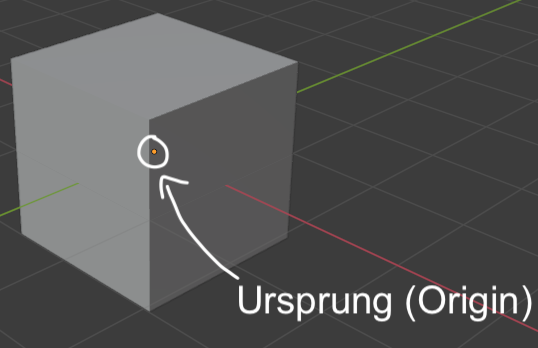
\includegraphics{Chapters/Images/Chapter_7/7_1_Origin.png}

\caption{\label{fig-1_1}Der orangene Punkt markiert den Ursprung
(Origin) eines Objektes.}

\end{figure}%

\marginnote{Position befindet sich am Ursprung des Objekts}

Die genaue Position des Objektes wird anhand eines kleinen orangen
Punktes im Viewport-Display angezeigt. Bei diesem Punkt handelt es sich
um den Ursprung des Objektes (Origin). Die Position eines Objektes
bezieht sich immer auf diesen orangen Punkt, selbst wenn das Mesh selbst
diese Position gar nicht abdeckt.

\section{Rotation}\label{rotation}

\marginnote{Rotation}

Die Rotation eines Objektes beschreibt, wie sehr das Objekt entlang der
drei Achsen rotiert wird. Analog zur Position ist die Rotation ebenfalls
in die drei Achsen X, Y und Z aufgeteilt. Beispielsweise führt eine
Veränderung der Rotation beim Wert X dazu, dass das Objekt entsprechend
entlang der X-Achse rotiert wird. Durch die Verwendung aller drei Achsen
können so komplexe Rotationen erfolgen. Indem alle Werte erneut auf 0
gesetzt werden, befindet sich das Objekt wieder in seiner Grundposition.

\marginnote{Drehpunkt der Rotation}

Der Ursprung des Objektes stellt den Drehpunkt für die Rotation mittels
der Sidebar dar. Das heisst, die Objekte werden jeweils um den
Ursprungspunkt herumrotiert. Dies wird beispielsweise deutlich, wenn
sich der Ursprungspunkt ausserhalb des Objektes befindet.

\section{Scale}\label{scale}

\marginnote{Skalierung}

Die Skalierung eines Objekts beschreibt, wie stark ein Objekt
vergrössert oder verkleinert wird. Diese Objekteigenschaft lässt sich
ebenfalls individuell für alle drei Achsen einstellen. So kann ein
Objekt entlang der X-Achse vergrössert werden, indem der dazugehörige
X-Wert auf einen Wert über 1 festgelegt wird. Werte im Bereich von
grösser als 0 und kleiner als 1 führen zu einer Verkleinerung des
Objektes entlang der entsprechenden Achse. Ein Wert von 0 führt dazu,
dass das Objekt entlang der entsprechenden Achse keine Grösse mehr hat
und aus der entsprechenden Perspektive dem entsprechend nicht mehr
sichtbar ist.

\marginnote{Bezugspunkt der Skalierung}

Analog zu der Position und der Rotation bezieht sich die Skalierung
ebenfalls auf den Ursprung des Objektes. Wenn sich das Mesh ausserhalb
des Ursprungs befindet, führt dies dazu, dass auch der Leerraum zwischen
dem Mesh und dem Ursprung entsprechend skaliert wird. Befindet sich die
Grenze eines Objektes etwa um den Wert 1 vom Ursprung entfernt, führt
eine Skalierung um den Wert 2 dazu, dass das Mesh selbst verdoppelt wird
-- allerdings wird die Distanz zum Ursprung des Objektes ebenfalls
verdoppelt.

\section{Dimension}\label{dimension}

\marginnote{Dimensionen von Objekten}

Unterhalb des Eingabefeldes für die Skalierung befindet sich ein
weiteres Feld, welches die Dimensionen eines 3D-Meshes basierend auf den
drei Achsen angibt. Die Dimensionen des Objektes sind direkt mit der
Skalierung des Objektes verbunden. Eine Veränderung der
X-Achsen-Dimension führt dazu, dass die Skalierung anhand der X-Achse so
angepasst wird, dass sie der eingegebenen Grösse des Objektes
entsprechen. Dadurch kann etwa direkt bestimmt werden, dass ein Objekt
entlang der verschiedenen Achsen eine bestimmte Grösse innehat, ohne
dass die Skalierung der entsprechenden Grösse angepasst wird.

\section{Transformationen sperren}\label{transformationen-sperren}

\marginnote{Transformationen sperren}

Neben den Werten für die Position, Rotation und Skalierung befinden sich
drei aufgeschlossene Schlösser. Durch das Anklicken dieser Schlösser
lässt sich die dazugehörige Eigenschaft auf einer Achse sperren, sodass
sie nicht mehr verändert werden kann. Das entsprechende Symbol verändert
sich dadurch zu einem geschlossenen Schloss.

\marginnote{Sperrung gilt nur für Viewport-Display}

Die Werte links neben dem Schloss lassen sich allerdings immer noch
verändern, was kontraintuitiv wirken mag. Dies liegt daran, dass sich
diese Sperrung auf Veränderungen mittels des Viewport Displays bezieht,
welche nun als Nächstes betrachtet werden.

Übung 3: Verwendung der Sidebar

\textbf{Übung 3.1}

Versuchen Sie den Standardwürfel so zu skalieren, dass er entsprechend
der Abbildung einen in die Höhe ragenden Quader darstellt.

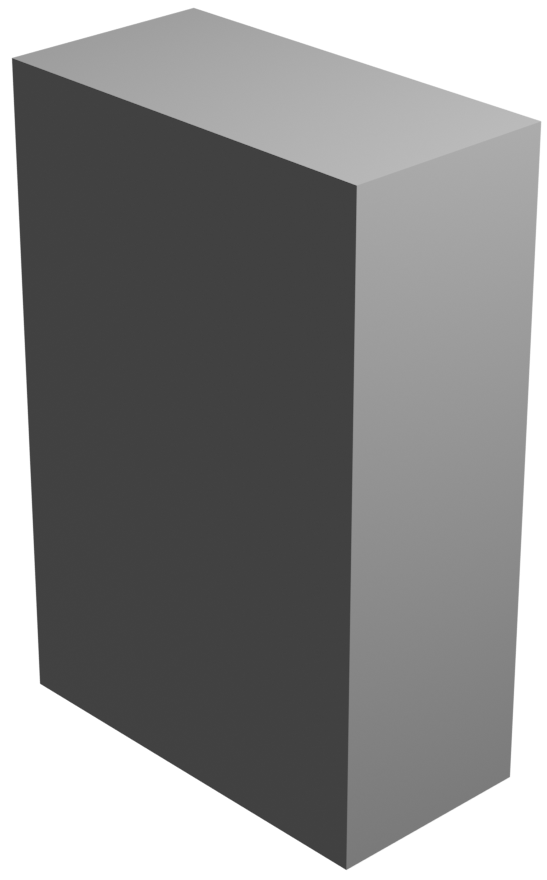
\includegraphics{Chapters/Images/Chapter_7/Exercise_3_1.png}

\textbf{Übung 3.2}

Versuchen Sie den Standardwürfel so zu verändern, dass er aus der
orthogonalen (Taste \kbd{5} ) Vorder/Rück-Ansicht (Taste \kbd{1} ) nicht
mehr sichtbar ist.

Merke\ldots{}

Die drei Transformationen Location, Rotation und Scale aus der Sidebar
beziehen sich alle drei jeweils auf den Ursprung des Objektes.

Dimension des Objektes hängt mit dessen Skalierung zusammen.

\chapter{Objekte im Viewport-Display
transformieren}\label{objekte-im-viewport-display-transformieren}

\marginnote{Befehle für Transformationen}

Statt mit der Sidebar können Objekte auch direkt im 3D-Viewport-Display
transformiert werden. Sobald ein Objekt -- oder auch mehrere Objekte --
ausgewählt sind, lassen sich die Objekte direkt im Viewport mittels der
folgenden Befehle transformieren:

\begin{itemize}
\tightlist
\item
  Position: \kbd{G} («Grab»)
\item
  Rotation: \kbd{R}
\item
  Skalierung: \kbd{S}
\end{itemize}

\section{Position}\label{position}

\marginnote{Objekte bewegen mittels \kbd{G}}

Durch das Drücken der Taste \kbd{G} lässt sich ein ausgewähltes Objekt
mit der Maus im Raum verschieben. Blender aktualisiert parallel die
Position des Objektes in der Sidebar, sodass diese klar nachvollziehbar
ist.

\marginnote{Bewegung entlang einer Achse}

Es ist auch im Viewport möglich, ein Objekt nur entlang einer Achse zu
bewegen. Hierfür wird nach dem Drücken der Taste \kbd{G} die Taste für
die entsprechende Achse festgelegt (\kbd{X},\kbd{Y} oder \kbd{Z}). Der
farbige Strich im Viewport-Display, welcher die entsprechende Achse
markiert, leuchtet dadurch heller auf. Wenn die Maus nun bewegt wird,
bewegt sich das Objekt lediglich entlang dieser Achse. Um die Bewegung
zu beenden oder zu bestätigen, wird entweder die linke Maustaste oder
die \kbd{Enter}-Taste gedrückt. Um die Transformation abzubrechen, kann
die rechte Maustaste oder die \kbd{esc}-Taste gedrückt werden. Das
Objekt wird dadurch wieder in seine Ursprungsposition zurückgestellt.

\marginnote{Bewegung entlang einer Achse sperren}

Es ist auch möglich, zwei Achsen gleichzeitig für eine Bewegung
auszuwählen. Dabei wird die Bewegung entlang einer Achse gesperrt,
sodass nur die beiden anderen Achsen für eine Bewegung freigegeben
werden. Hierfür wird die Taste \kbd{Shift}in Kombination mit der Taste
für die zu sperrende Achse (\kbd{X},\kbd{y} oder \kbd{Z}) gedrückt. Wenn
ein Objekt also lediglich entlang der X- und Y-Achse bewegt werden soll,
aber die Z-Achse nicht verändert werden soll, kann nach dem Drücken der
Taste \kbd{G} bei gedrückter \kbd{Shift}-Taste die Z-Achse mittels der
Taste \kbd{Z} gesperrt werden.

\marginnote{Bewegung mittels Zahlen präzise angeben}

Statt mit der Maus kann während des Bewegungsvorgangs eine Zahl
eingegeben werden, um eine Bewegung zu quantifizieren. Soll ein Objekt
etwa um 2 Meter entlang der X-Achse verschoben werden, so wird, nachdem
die Bewegung mittels der Taste \kbd{G} gestartet und mittels der Taste
\kbd{X} auf die X-Achse festgelegt wird, die Taste \kbd{2} gedrückt, um
die Bewegung auf 2 Meter festzulegen. Durch das gleichzeitige Drücken
der Taste \kbd{-} können auch negative Werte eingegeben werden, sodass
die Bewegung in die entgegengesetzte Richtung geschieht. In der linken
oberen Ecke des Viewport Displays wird jeweils die entsprechende Zahl
angezeigt. Es ist zudem möglich, Zahlenangaben mit Dezimalstellen für
Bewegungen einzugeben.

\section{Rotation}\label{rotation-1}

\marginnote{Objekte rotieren mittels \kbd{R}}

Um ein ausgewähltes Objekt mit der Maus zu rotieren, wird die Taste
\kbd{R} gedrückt. Wie auch bei der Bewegung lässt sich eine
Transformation entlang einer Achse ansteuern, indem die Taste für die
entsprechende Achse gedrückt wird (\kbd{X},\kbd{Y} oder \kbd{Z}). Ebenso
lässt sich eine Achse für die Rotation sperren, indem die entsprechende
Taste für diese Achse bei gedrückter \kbd{Shift}-Taste gedrückt wird.
Wenn nun also ein Objekt entlang der Z-Achse rotiert werden soll, wird
zunächst das entsprechende Objekt ausgewählt und anschliessend die Taste
\kbd{R}für den Befehl der Rotation gedrückt. Indem die Taste \kbd{R}
anschliessend gedrückt wird, lässt sich das Objekt nun lediglich entlang
der Z-Achse rotieren. Während der Rotation verändert sich die Form der
Maus und sie ist mit einem Strich zu dem Punkt, um den die Rotation
erfolgt, verbunden. In der Regel handelt es sich dabei um den Ursprung
des Objektes. Allerdings kann die Rotation im Viewport-Display auch
hinsichtlich anderer Punkte im Raum erfolgen -- dies wird in einem
späteren Kapitel ausführlicher beschrieben.

\marginnote{Präzise Rotation mittels Zahlen}

Auch während der Rotation kann mit der Eingabe von Zahlen gearbeitet
werden. Um ein Objekt beispielsweise um 45 Grad entlang der Z-Achse zu
drehen, wird nach dem Start der Rotation mittels der Taste \kbd{R} und
der Festlegung der Z-Achse mit der Taste \kbd{Z} die Zahl 45 mittels der
Tasten \kbd{4} \kbd{5} eingegeben. Auch hier lässt sich die Richtung
umkehren, indem die Taste \kbd{-} gedrückt wird.

\section{Scale}\label{scale-1}

\marginnote{Objekte Skalieren mittels \kbd{S}}

Um ein ausgewähltes Objekt mit der Maus zu skalieren, wird die Taste
\kbd{S} gedrückt. Wie auch bei der Bewegung und der Rotation lässt sich
eine Transformation entlang einer einzelnen Achse ansteuern, indem die
Taste für die entsprechende Achse gedrückt wird (\kbd{X},\kbd{Y} oder
\kbd{Z}). Ebenso lässt sich eine Achse für die Rotation sperren, indem
die entsprechende Taste für diese Achse bei gedrückter \kbd{Shift}-Taste
gedrückt wird.

\marginnote{Skalierung entlang einer Achse}

Um ein Objekt nur entlang der X-Achse zu vergrössern oder zu
verkleinern, wird nach der Auswahl des Objektes die Taste \kbd{S}
gedrückt, um mit der Skalierung zu starten. Anschliessend kann durch das
Drücken der Taste \kbd{X} festgelegt werden, dass die Transformation
lediglich entlang der X-Achse vollzogen werden soll. Während der
Skalierung verändert sich der Mauszeiger ebenfalls. Zudem ist er mittels
eines Striches mit dem Punkt verbunden, zudem hin sich die Skalierung
orientiert. Wird die Maus näher zu diesem Punkt bewegt, verkleinert sich
das Objekt. Wenn die Maus von diesem Punkt weiter entfernt wird,
vergrössert sich das Objekt.

\marginnote{Präzise Skalierung mittels Zahlen}

Die Skalierung kann mittels Zahleneingaben ebenfalls sehr genau
vorgenommen werden. Um ein Objekt etwa in seiner Grösse zu verdoppeln,
kann nach dem Start der Transformation mittels der Taste \kbd{S} die
Zahl \kbd{2}eingegeben werden. Dadurch wird das Objekt um den Faktor 2
vergrössert. Auch hier lässt sich ein negativer Wert mittels der Taste
\kbd{-} festlegen. Dies führt dazu, dass das Objekt durch seinen
Bezugspunkt hindurch in die andere Richtung skaliert und gespiegelt
wird. Während dies bei symmetrischen Objekten zu keinem bemerkbaren
Unterschied führt, wird der Effekt bei asymmetrischen Objekten deutlich.

Übung 4 : Objekttransformationen

\textbf{Übung 4.1}

Skalieren Sie einen Würfel entlang der X-Achse auf seine halbe Grösse.

\textbf{Übung 4.2}

Bilden Sie das unten abgebildete Objekt nach.

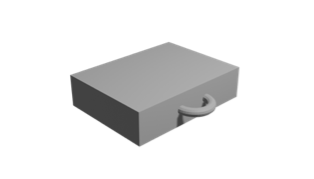
\includegraphics{Chapters/Images/Chapter_8/Exercise_4_2.png}

Merke\ldots{}

Mittels der Tasten \kbd{G},\kbd{R} und \kbd{S} lassen sich Objekte auch
im Viewport-Display bewegen, rotieren und skalieren.

Mittels der Eingabe von Zahlen können Bewegungen, Rotationen und
Skalierungen genau vorgenommen werden.

Mittels der Tasten \kbd{X},\kbd{Y} und \kbd{Z} können Transformationen
auf der eine Achse festgelegt werden.

Mittels der Tasten \kbd{X},\kbd{Y} und \kbd{Z} bei gedrückter
\kbd{Shift}-Taste können Transformationen auf der entsprechenden Achse
unterbunden werden.

\chapter{Object- und Edit-Mode}\label{object--und-edit-mode}

\section{Die verschiedenen
Bearbeitungs-Modi}\label{die-verschiedenen-bearbeitungs-modi}

\marginnote{Object-Mode}

Die bisherigen Transformationen, die an Objekten gemacht wurden, haben
sich immer auf den Object-Mode bezogen. Dabei wurden grundlegende
Eigenschaften von Objekten (Position, Rotation und Skalierung)
verändert. Die Form des Objektes selbst wurde dabei nicht verändert,
sondern lediglich seine Darstellungsweise. Durch das Zurücksetzen der
Werte in der Sidebar erscheint das Objekt wieder in seiner
ursprünglichen Form.

\begin{tipp}{Weiterführende Informationen}
Das Zurücksetzen der Transformationen kann direkt mittels folgenden Shortcuts erfolgen:  Zurücksetzen der Position: \kbd{Alt} + \kbd{G}  Zurücksetzen der Rotation: \kbd{Alt} + \kbd{R}  Zurücksetzen der Skalierung: \kbd{Alt} + \kbd{S}
\end{tipp}

Durch die bisherigen Transformationen wurde das Objekt als Ganzes
bearbeitet. Dies zeichnet die Transformationen im Object-Mode aus. Nebst
dem Object-Mode gibt es noch eine Reihe anderer Modi. In der oberen
linken Ecke des Viewports ist jeweils ersichtlich, welcher Modus gerade
verwendet wird. Durch einen Klick auf das Dropdown-Menü erscheint eine
Liste der verfügbaren Modi:

\marginnote{Die verschiedenen Bearbeitungs-Modi}

\begin{itemize}
\item
  \textbf{Object Mode}: In diesem Modus können die Objekte in einer
  Szene als Ganzes transformiert und angeordnet werden.
\item
  \textbf{Edit Mode}: In diesem Modus können die einzelnen Bestandteile
  des Objekts anvisiert und bearbeitet werden.
\item
  \textbf{Sculpt Mode}: In diesem Modus kann das Objekt anhand von
  Sculpting-Tools bearbeitet werden.
\item
  \textbf{Vertex Paint}: In diesem Modus werden einzelne Punkte des
  Objekts angesteuert und mit Attributen versehen.
\item
  \textbf{Weight Paint}: In diesem Modus werden dem Objekt verschiedene
  Gewichte aufgemalt, welche anschliessend für weitere Funktionen
  verwendet werden können.
\item
  \textbf{Texture Paint}: In diesem Modus ist es möglich, ein Objekt mit
  einer Textur zu bemalen.
\end{itemize}

\marginnote{Wechsel zwischen Object- und Edit-Mode}

Im Rahmen dieses Kurses wird vorwiegend mit dem Object- und dem
Edit-Mode gearbeitet. Der Wechsel zwischen diesen beiden Modi stellt
einen wichtigen Wechsel zwischen den Modi dar. Deshalb ist es möglich,
mittels einer einzigen Taste zwischen dem Object- und dem Edit-Mode hin-
und herzuwechseln -- nämlich mittels der Taste \kbd{Tab} . Dabei wird in
den Edit-Mode für das aktuell ausgewählte Objekt gewechselt. Für
Objekte, welche nicht aus einzelnen Komponenten bestehen (beispielsweise
Kameras oder Lichtquellen), ist kein Edit-Mode verfügbar.

\section{Struktur von 3D-Meshes}\label{struktur-von-3d-meshes}

\marginnote{Der Gitteraufbau von 3D-Meshes}

Beim Wechseln in den Edit-Mode erscheint das Mesh in seiner Struktur,
bestehend aus mehreren Polygonen. Dabei handelt es sich um einzelne
Oberflächenstrukturen der Meshes. Die Polygone -- und somit auch das
Mesh -- bestehen in ihrer Struktur aus folgenden Elementen:

\begin{itemize}
\tightlist
\item
  \textbf{Vertices}: Einzelne Punkte in einem Mesh
\item
  \textbf{Edges}: Linien zwischen zwei Vertices in einem Mesh
\item
  \textbf{Faces}: Flächen zwischen mehreren Edges/Vertices in einem Mesh
\end{itemize}

\begin{figure}[H]

{\centering 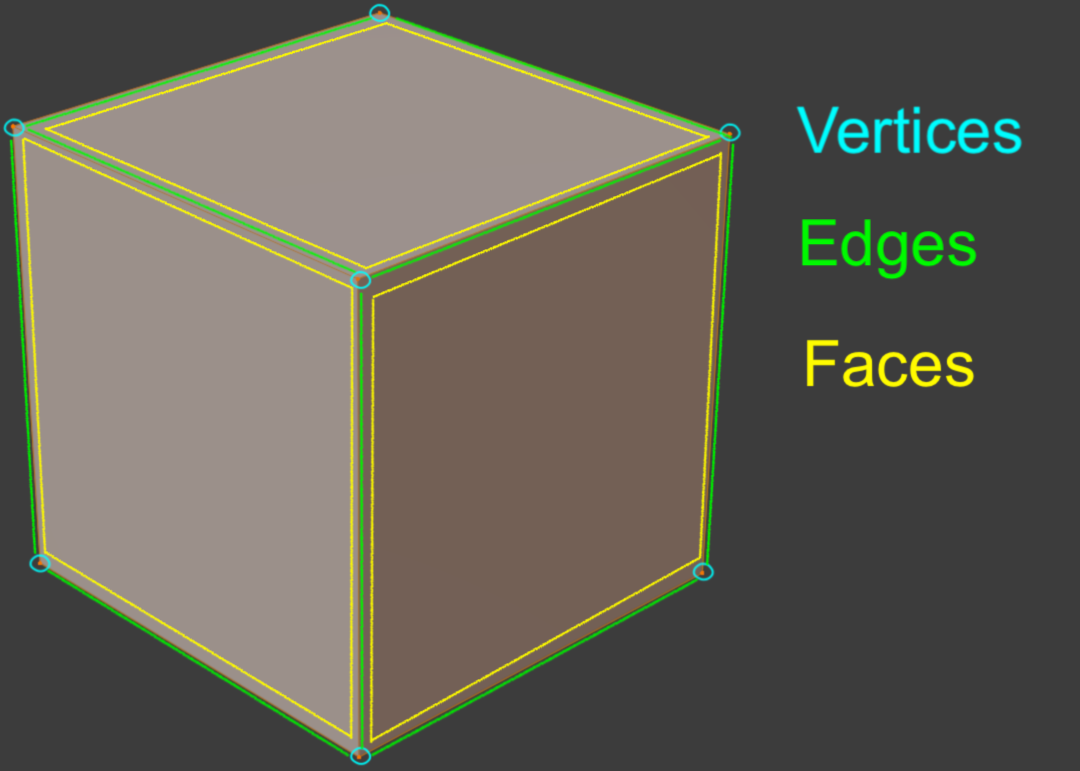
\includegraphics{Chapters/Images/Chapter_9/9_1_Vertices_Edges_Faces.png}

}

\caption{Vertices, Edges und Faces.}

\end{figure}%

\marginnote{Select-Modus wechseln}

Im Edit-Mode können wahlweise Vertices, Edges oder Faces ausgewählt
werden, je nachdem in welchem Select-Modus man sich befindet. Die drei
Select-Modi sind in der linken oberen Ecke direkt neben dem Auswahlfeld
für den Bearbeitungs-Modus (in dem Fall der Edit-Mode) aufzufinden.

\begin{figure}

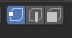
\includegraphics{Chapters/Images/Chapter_9/9_2_ Select_Mode_Choice.png}

\caption{\label{fig-1_2}Schaltfläche für den Vertex-, Edge- und
Face-Select-Modus in der linken oberen Ecke des Edit-Modes.}

\end{figure}%

\subsection{Vertices}\label{vertices}

\marginnote{Vertices}

Ein Vertex (Mehrzahl: Vertices) stellt die grundlegendste Einheit in
einem Mesh dar. Jeder Vertex beschreibt einen Punkt in einem Mesh.
Anders als die Objekte als Ganzes, verfügen Vertices nur über das
Merkmal ihrer jeweiligen Position. Die Merkmale Skalierung und Rotation
gibt es für Vertices nicht. Ein Vertex hat deshalb auch keine
Dimensionen.

\marginnote{Auswahl von Vertices}

Werden zwei miteinander verbundene Vertices ausgewählt, so wird
automatisch auch das dazwischenliegende Edge ausgewählt. Ebenso wird
automatisch das dazugehörige Face mit ausgewählt, wenn alle Vertices
dieses Faces ausgewählt werden. Ein einzelner Vertex kann lediglich im
Vertex Select-Modus angewählt werden.

\subsection{Edges}\label{edges}

\marginnote{Edges}

Edges beschreiben Linien, welche zwischen zwei Vertices liegen. Da ein
Edge genau der Verbindung zwischen zwei Vertices entspricht, ist dessen
Mittelpunkt identisch zur Mitte zwischen den beiden Vertices.

\marginnote{Auswahl von Edges}

Im Edge-Select-Modus können die Edges als solche ausgewählt werden.
Dabei werden automatisch auch die beiden zum Edge dazugehörigen Vertices
ausgewählt. Wenn alle Edges eines Faces ausgewählt werden, dann wird
automatisch auch das dazugehörige Face ausgewählt.

\subsection{Faces}\label{faces}

\marginnote{Faces}

Faces stellen die Flächen zwischen verbundenen Edges/Vertices dar. Die
Position des Faces entspricht dem Mittelpunkt dieser Fläche und somit
dem Mittelpunkt der dazugehörigen Vertices. Es ist allerdings auch
möglich, dass mehrere Vertices mittels Edges verbunden sind, ohne eine
Fläche zu beinhalten.

Mittels des Face-Select-Modus können Faces direkt angewählt werden.
Alternativ kann ein Face auch angewählt werden, indem im
Vertex-Select-Modus alle zum Face dazugehörigen Vertices ausgewählt
werden, oder indem im Edge-Select-Modus alle zum Face dazugehörigen
Edges ausgewählt werden.

\section{Anzahl Vertices in einem
Face}\label{anzahl-vertices-in-einem-face}

\begin{tipp}{Weiterführende Informationen}
Polygone und Faces sind in ihrer Bedeutung praktisch deckungsgleich. Faces beschreiben jedoch eher die Fläche eines Polygons, während das Polygon eher die Gesamtheit von Vertices, Edges und Faces beschreibt. Der Begriff Polygon wird innerhalb von Blender allerdings selten verwendet.
\end{tipp}

\marginnote{Anzahl Vertices in einem Face}

Der Default-Cube, den Blender jeweils beim Start eines neuen Projektes
zur Verfügung stellt, besteht aus sechs Faces. Jedes dieser Faces
beinhaltet vier Vertices. Es ist allerdings auch möglich, dass ein Face
aus mehr oder weniger Vertices besteht. Es gibt verschiedene Begriffe,
basierend auf der Anzahl Vertices in einem Face:

\marginnote{Bezeichnung von Faces aufgrund Anzahl Vertices}

\begin{itemize}
\tightlist
\item
  \textbf{Triangles} (\textbf{Tris}): Faces, die aus drei Vertices
  bestehen
\item
  \textbf{Quadrangles} (\textbf{Quads}): Faces, die aus vier Vertices
  bestehen
\item
  \textbf{N-Gons}: Faces, die aus n Vertices bestehen
\end{itemize}

\begin{figure}

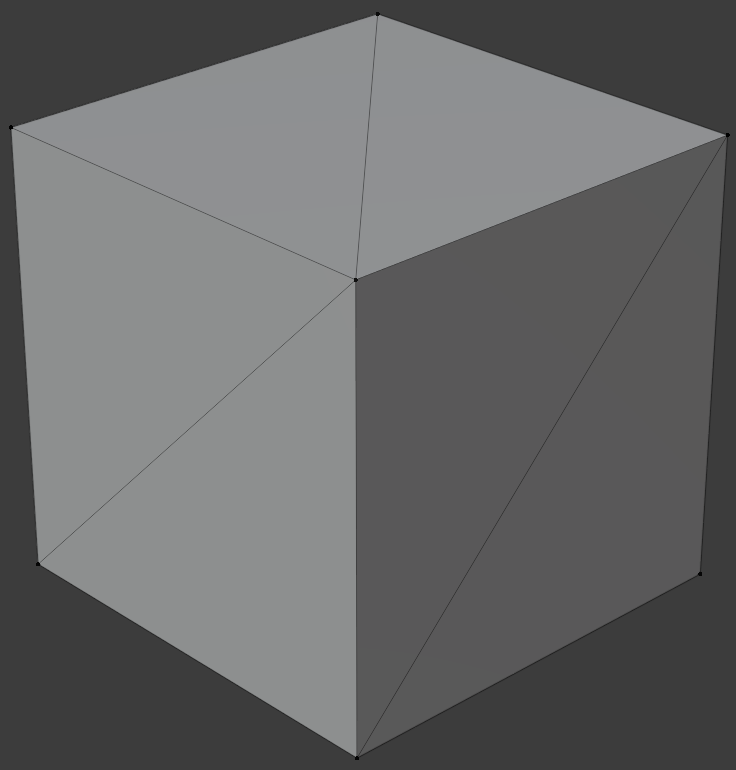
\includegraphics{Chapters/Images/Chapter_9/9_3_Cube_ Tris.png}

\caption{\label{fig-1_3}Der Standardwürfel bestehend aus Tris statt aus
Quads.}

\end{figure}%

\marginnote{Tris aus Quads ableiten}

Aus Quads lassen sich sehr einfach Tris bilden. Hierfür muss lediglich
jedes Quad zwischen zwei gegenüberliegenden Vertices zerschnitten
werden, sodass die Fläche in zwei Dreiecke unterteilt wird. Beim Rendern
von Bildern werden Quads in den 3D-Objekten automatisch in Tris
unterteilt, was im Normalfall für den Benutzer jedoch kaum ersichtlich
ist.

\marginnote{Bevorzugung von Quads}

Trotzdem ist es sinnvoll, sich beim Modellieren von 3D-Objekten eher an
die Verwendung von Quads zu gewöhnen. Viele Tricks und Kniffe der
Objektbearbeitung lassen sich einfacher oder teilweise sogar nur auf
Quads anwenden. Somit erleichtert die Arbeit mit Quads den
Arbeitsprozess erheblich. Weiterhin sind Quads auch in vielen
Animationsstudios der Standard.

\begin{figure}

\includegraphics{Chapters/Images/Chapter_9/9_4_Prof_Figures.png}

\caption{\label{fig-1_4}Links eine gerenderte 3D-Figur und rechts die
Figur in ihrer Gitterstruktur.}

\end{figure}%

\marginnote{Anwendung von Tris}

Arbeiten mit Tris ist trotzdem durchaus möglich und vereinzelte Tris in
Objekten sind auch nicht problematisch. In manchen Situationen sind Tris
sogar flexibler als Quads. Wenn allerdings die Objekte komplett aus Tris
bestehen sollen, macht dies gerade in gemeinschaftlichen Prozessen nur
Sinn, wenn alle beteiligten Personen mit Tris umgehen können.

Merke\ldots{}

Vertices beschreiben die einzelnen Punkte in einem 3D-Objekt.

Edges beschreiben die verbundenen Punkte in einem 3D-Objekt.

Faces beschreiben Flächen zwischen mehr als zwei verbundenen Vertices.

Faces mit vier Vertices (Quads) sind gegenüber Faces mit drei Vertices
(Tris) in den meisten Fällen zu bevorzugen.

\section{Auswahl von Vertices, Edges und Faces im
Edit-Mode}\label{auswahl-von-vertices-edges-und-faces-im-edit-mode}

\marginnote{Auswahl von Vertices, Edges und Faces im Edit-Mode}

Abhängig davon, welcher Select-Modus gerade aktiviert ist, lassen sich
entweder die Vertices, Edges oder Faces auswählen. Die Auswahl der
jeweiligen Elemente geschieht mittels der linken Maustaste. Wie auch im
Object-Mode können bei gedrückter \kbd{Shift}-Taste zusätzliche Elemente
ausgewählt werden. Ebenso können mit der Taste \kbd{C} der
Circle-Select-Modus und mittels der Taste \kbd{B} der Box-Select-Modus
verwendet werden. Zudem kann mit der Tastenkombination \kbd{Ctrl} +
\kbd{I} die Auswahl umgekehrt werden.

\marginnote{Select linked mittels \kbd{L}}

Im Edit-Mode gibt es weitere Auswahl-Optionen. Wenn sich der Mauszeiger
über einem Element eines Objekts befindet, können mit der Taste \kbd{L}
alle Elemente, welche über Edges damit verbunden sind, ausgewählt
werden. Dies ermöglicht es, alle verbundenen Elemente auszuwählen. Um
alle Elemente eines Objektes -- also auch unverbundene Elemente --
auszuwählen, kann die Taste \kbd{A} gedrückt werden.

\marginnote{Edge-Loop-Select bei gedrückter Taste \kbd{Alt}}

Weiterhin lassen sich ganze Verbindungen von Edges auswählen, wenn die
Taste \kbd{Alt} während der Auswahl gedrückt wird. Dadurch werden alle
Edges, die gemeinsam eine Linie mit dem gerade ausgewählten Element
bilden, ausgewählt. Dies ist auch im Vertex-Select-Modus möglich. Im
Face-Select-Modus werden alle Faces, die gemeinsam eine Linie bilden,
ausgewählt (hierfür muss der Mausklick allerdings bei einem Edge
erfolgen -- nicht in der Fläche des Faces).

\section{Das Innere des Objekts}\label{das-innere-des-objekts}

\marginnote{Virtuelle Objekte haben meist keine Füllung}

So wie auch in der realen Welt haben virtuelle 3D-Objekte Flächen,
welche aus mindestens drei Kanten bestehen und mindestens drei Ecken. Im
Gegensatz zu Objekten in der realen Welt bestehen virtuelle Objekte
nicht aus einer Füllung. Wird ein realer Apfel mit einem Messer in der
Mitte geteilt, so wird der Inhalt unter der Schale -- etwa das
Fruchtfleisch oder das Kerngehäuse -- sichtbar. Bei einem 3D-Mesh gibt
es jedoch kein Inneres, sodass lediglich die Oberflächen der äusseren
Struktur von der anderen Seite aus ersichtlich werden. Das Mesh besteht
somit nur aus der Oberfläche, welche ein leeres Volumen überdeckt.

Aus dem Umgang mit realen Objekten ist der Mensch sich gewohnt, dass
Objekte einen Inhalt haben. Dies trifft auf digitale Objekte selten zu.
Als Betrachter von digitalen Objekten ist dieser Sachverhalt nur in den
seltensten Fällen bemerkbar. Dadurch wird durch fehlende
Auseinandersetzung mit dieser Thematik die Illusion eines möglichen
Inhaltes verstärkt.

\marginnote{Wenn das Innere sichtbar wird}

In Videospielen kann es vorkommen, dass die Kamera durch einen Fehler in
ein Objekt hineingelangt. Dadurch wird das Objekt anschliessend von der
Innenseite aus betrachtet. Dies muss allerdings nicht immer der Fall
sein. In manchen Situationen ist dieses Objekt gar nicht mehr sichtbar,
wenn es von innen betrachtet wird.

\section{Normalen: die richtige Seite der Faces
finden}\label{normalen-die-richtige-seite-der-faces-finden}

\marginnote{Die zwei Seiten von Faces}

Da 3D-Meshes keinen inneren Hohlraum haben, bilden die Faces die
Oberfläche, welche das Objekt abdeckt. Dies bedeutet aber auch, dass es
zwei Seiten von dieser Oberfläche geben muss: eine Seite, die betrachtet
werden soll, und eine, die nicht betrachtet werden soll. In den meisten
Fällen ist schnell klar, welche Seite eines Objektes von Bedeutung ist.
Einen Apfel betrachtet man jeweils von aussen, also ist die nach aussen
gerichtete Seite jene Seite, welche betrachtet werden soll. Ebenso
verhält es sich bei einem Charakter. In diesem Fall ist ebenfalls die
nach aussen gerichtete Seite von Bedeutung und nicht das Innere seines
Körpers.

\begin{tipp}{Weiterführende Informationen}
Bei bestimmten Einstellungen werden die Rückseiten der Oberflächen von Objekten fehlerhaft dargestellt. In diesen Fällen hilft es oftmals, die Ausrichtung der Normalen zu überprüfen und bei Bedarf anzupassen.  In manchen Game-Engines werden die Rückseiten von Objekten in den Grundeinstellungen gar nicht angezeigt. Dadurch blickt man bei den Oberflächen mit der falschen Ausrichtung durch das Objekt hindurch. Dies vermittelt den Eindruck, dass ein Teil des Objekts fehlen würde. Dieser Teil ist noch da – allerdings der falschen Richtung zugewendet.
\end{tipp}

\marginnote{Die zu betrachtende Seite eines Würfels}

Wie verhält es sich bei Blenders Standardwürfel? Bei diesem wird
zunächst die Aussenseite betrachtet. Allerdings wäre es auch möglich,
dass der Default-Cube von innen betrachtet werden soll -- etwa, wenn
eine Szene im Inneren eines Raumes dargestellt werden soll und der
Würfel die Wände, den Boden und die Decke des Raumes darstellt. In
diesem Fall ist nicht mehr die Aussenseite des Würfels relevant, sondern
die Innenseite.

\marginnote{Normalen}

Die Normalen eines Objektes geben jeweils an, in welche Richtung
Vertices, Edges und Faces gerichtet sind. Wenn ein Würfel etwa von innen
betrachtet werden soll, müssen die Normalen nach innen gekehrt werden.
Wenn der Würfel allerdings als solcher von aussen betrachtet werden
soll, dann müssen die Normalen nach aussen gekehrt sein.

\marginnote{Normalen darstellen}

Die Normalen eines 3D-Objektes lassen sich im Edit-Mode betrachten,
indem die entsprechende Ansicht aktiviert wird. Diese wird im
Dropdown-Menü zu den Viewport-Overlays in der rechten oberen Ecke des
3D-Viewports unter dem Abschnitt «\emph{Normals}» mit der Schaltfläche
«\emph{Display Normals}» aktiviert. Anschliessend erscheinen in den
Faces kleine blaue Striche, welche in diejenige Richtung zeigen, gegen
die das Face dargestellt ist.

\begin{figure}


\includegraphics{Chapters/Images/Chapter_9/9_5_Icon_Normals.png}

\caption{\label{fig-1_5}Icon zur Darstellung der Normalen in den
Viewport-Overlays.}

\end{figure}%

\marginnote{Face-Orientation darstellen}

Es ist auch möglich, in den Viewport-Overlays die «\emph{Face
Orientation}» zu aktivieren. Dadurch werden die Oberflächen eines
Objekts in blauer Farbe dargestellt, wenn es sich um die Seite der
Normalen handelt, oder in roter Farbe, wenn es sich um die Seite ohne
Normalen handelt. Diese Ansicht ist auch im Object-Mode verfügbar,
allerdings nur in der Solid-Ansicht und wenn X-Ray deaktiviert ist.

\marginnote{Normalen umkehren und neu berechnen}

Wenn alle Faces innerhalb eines Objekts ausgewählt werden, kann mittels
der Tastenkombination \kbd{Alt} + \kbd{N} das Menü «\emph{Normals}» beim
Mauszeiger geöffnet werden. Mit der Option «\emph{Flip}» können
anschliessend alle Normalen in die umgekehrte Richtung gekehrt werden.
Zudem können die Normalen mittels der Option «\emph{Recalculate
Outside}» zur äusseren Seite hin oder mittels «\emph{Recalculate
Inside}» zur inneren Seite hin berechnet werden.

\chapter{Einstieg in den Edit-Mode}\label{einstieg-in-den-edit-mode}

Ein Grossteil der Bearbeitungsmöglichkeiten, welche im Object-Mode mit
Objekten möglich sind, kann im Edit-Mode auch auf die Strukturelemente
der Objekte angewendet werden.

\section{Grab, Scale, Rotate}\label{grab-scale-rotate}

\marginnote{Ein Vertex kann nur bewegt werden}

Wenn ein einzelner Vertex ausgewählt wird, sind die
Transformationsmöglichkeiten relativ beschränkt. Mittels der Taste
\kbd{G} lässt sich der Vertex im dreidimensionalen Raum verschieben. Da
der Vertex allerdings nur einen isolierten Punkt ohne eine Dimension
darstellt, kann er weder skaliert, noch rotiert werden. Dementsprechend
wird in der Sidebar lediglich die Position des Vertex angegeben, während
die Skalierung und Rotation -- anders als im Object-Mode -- nicht
angegeben werden.

\marginnote{Skalierung und Rotation geschieht um den Median der Auswahl}

Sobald zwei Vertices ausgewählt werden, wird in der Sidebar nicht mehr
die Position der einzelnen Vertices angegeben, sondern die Position des
Medians zwischen diesen beiden Vertices. Dies ist unabhängig davon, ob
die Vertices mittels Edges oder Faces miteinander verbunden sind oder
nicht. Mittels der Taste \kbd{R} oder \kbd{S} kann die Auswahl rotiert
oder skaliert werden. Beide Transformationen beziehen sich dabei auf den
Median zwischen diesen beiden Vertices. Wird also beispielsweise eine
Skalierung um den Faktor 2 getätigt (mittels der Tasten \kbd{S} und
\kbd{2}), verdoppelt sich der Abstand der beiden Vertices zum Median.
Rotationen führen dazu, dass die Vertices ebenfalls um den Median
rotiert werden.

\marginnote{Skalierung und Rotation verändert Position von Vertices}

Dadurch lässt sich bereits ein wichtiges Merkmal der Bearbeitung im
Edit-Mode betrachten: Mittels einer Skalierung lässt sich die Distanz
zwischen zwei Vertices verändern und dadurch auch ihre Position. Ebenso
werden Vertices bei der Rotation relativ zueinander im Raum rotiert und
so in ihren Positionen verändert. Dies macht auch einen Abschnitt für
die Skalierung oder Rotation in der Sidebar obsolet, da jegliche
Transformation lediglich zu einer Veränderung der individuellen
Platzierung der Vertices führt.

Anstatt der Vertices können auch Edges und Faces direkt angewählt
werden. Dabei werden automatisch die dazugehörigen Vertices mit
ausgewählt. Die Transformationen beziehen sich immer noch auf den
räumlichen Mittelpunkt zwischen den einzelnen Vertices, weshalb auch in
diesem Modus eine Skalierung oder Rotation zu einer Veränderung der
Positionen dieser Vertices führen.

Merke\ldots{}

Wie auch im Object-Mode können Vertices, Edges und Faces mittels der
Taste \kbd{G} bewegt, mittels der Taste \kbd{S} und mittels der Taste
\kbd{R} rotiert werden.

Skalierungen und Rotationen im Edit-Mode führen lediglich zu einer
Veränderung der Positionen der einzelnen Vertices basierend auf dem
Median der Vertex-Positionen.

\section{Add, Delete, Dissolve}\label{add-delete-dissolve}

\marginnote{Primitives innerhalb eines Objektes hinzufügen}

Innerhalb eines Objektes im Edit-Mode können weitere Mesh-Primitives
hinzugefügt werden. Dies geschieht wie im Object-Mode mit der
Tastenkombination \kbd{Shift} + \kbd{A}. Die Auswahl ist allerdings nur
noch auf Mesh-Primitives beschränkt. Dementsprechend ist es nicht
möglich, einem Mesh im Edit-Mode ein Kurven-Objekt anzufügen. Allerdings
stehen alle primitiven Formen der Meshes zur Verfügung. Wie auch im
Object-Mode werden die Objekte an der Position des 3D-Cursors
hinzugefügt.

\marginnote{Elemente löschen mit \kbd{X}}

Wie auch im Object-Mode können im Edit-Mode ausgewählte Elemente
gelöscht werden, indem die Taste \kbd{X} oder \kbd{Delete} gedrückt
wird. Anders als im Object-Mode erscheint bei beiden Tasten ein Menü
beim Mauszeiger, allerdings weil in diesem Fall der Löschvorgang
präzisiert werden muss. So lassen sich jeweils die ausgewählten Faces,
die ausgewählten Edges oder die ausgewählten Vertices löschen.

\marginnote{Elemente, welche beim Löschen eben falls entfernt werden}

Wird etwa beim Default-Cube eine einzelne Fläche ausgewählt und das Face
gelöscht, so bleiben die Edges, welche sich um die Fläche bilden,
erhalten -- lediglich das ausgewählte Face wird gelöscht. Wenn
allerdings die Edges gelöscht werden, verschwinden alle Edges, welche
das ausgewählte Face bilden -- lediglich die Vertices bleiben bestehen.
Durch die fehlenden Edges verschwinden nun allerdings auch die
angrenzenden Faces, da diesen nun je ein Edge fehlt. Wenn stattdessen
die Vertices gelöscht werden, fehlen auch für die angrenzenden Edges die
Bezugspunkte. Als Folge bleibt nur noch die gegenüberliegende Fläche
bestehen.

\marginnote{Faces und Edges isoliert löschen}

Bei der Auswahl von mehreren Flächen oder Edges kann das Löschen von
Elementen zu grösseren Veränderungen führen. So werden beim Löschen von
mehreren aneinandergereihten Faces auch die Edges, welche die Faces
abgrenzen, gelöscht. Um dies zu verhindern kann beim Löschen die Option
«\emph{Only Faces}» ausgewählt werden. Dadurch bleiben die Edges
bestehen. Zudem gibt es die Option «\emph{Only Edges \& Faces}» um
lediglich die einzelnen Vertices zu erhalten.

\marginnote{Elemente auflösen}

Nebst dem Löschen von Elementen besteht auch die Auswahl, dass Elemente
aufgelöst werden. Hierfür wird die Option «\emph{Dissolve}» im
Lösch-Menü angeboten. Dadurch werden die ausgewählten Elemente gelöscht
und die benachbarten Elemente anschliessend verbunden. Wird ein
einzelnes Edge ausgewählt, welches zwischen zwei Faces liegt, werden die
beiden Faces durch das Auflösen zu einem Face kombiniert. Ähnlich
verhält es sich beim Auflösen von Faces und Vertices.

\section{Duplicate}\label{duplicate}

\marginnote{Duplizieren mittels \kbd{D}}

Auch im Edit-Mode können Elemente mittels der Taste dupliziert werden,
wenn sie vorgängig ausgewählt wurden. Nach dem Tastendruck ist es direkt
möglich, die Objekte zu bewegen und mittels der linken Maustaste,
\kbd{Enter}- oder \kbd{Space}-Taste zu platzieren. Mittels der Taste
\kbd{esc} oder der rechten Maustaste kann diese Bewegung abgebrochen
werden und das Objekt wird an seine ursprüngliche Position
zurückgesetzt. Dadurch ist allerdings oftmals nicht mehr ersichtlich,
dass sich ein Duplikat an der Stelle des Originals befindet. Deshalb ist
es sinnvoll, in einem solchen Fall die letzte Aktion -- also das
Duplizieren -- ruckgängig zu machen oder das Duplikat direkt zu löschen.
Empfehlenswert ist es auch, die Elemente trotzdem an einer anderen
Stelle zu platzieren und sie dann erst zu löschen. Dadurch lässt sich
erkennen, dass die Elemente dupliziert wurden und noch gelöscht werden
müssen.

\section{Globale vs.~lokale
Koordinaten}\label{globale-vs.-lokale-koordinaten}

\marginnote{Globale Koordinaten}

Im Edit-Mode gibt es zwei Arten von 3D-Koordinaten, mit denen die
Position eines Vertex -- respektive der Median der Auswahl mehrerer
Vertices -- angegeben wird: die globalen und die lokalen Koordinaten.
Die globalen Koordinaten entsprechen denselben Koordinaten, die auch im
Object Mode verwendet werden. Diese beziehen sich auf den Ursprung der
Welt, welcher sich an der Position 0 aller drei Achsen befindet. Dabei
handelt es sich auch um den Punkt, an dem sich die Achsen im 3D-Viewport
kreuzen.

\marginnote{Lokale Koordinaten}

Die lokalen Koordinaten beziehen sich jeweils auf die Koordinaten des
aktuellen Objektes. Das heisst, dass diese Koordinaten sich immer auf
den Ursprung des Objektes beziehen. Wenn sich der Ursprung des Objektes
am Nullpunkt aller drei Achsen befindet und keine Skalierung oder
Rotation auf das Objekt angewendet wird, dann sind die globalen und die
lokalen Koordinaten identisch. Wenn sich der Ursprung allerdings an
einer anderen Stelle im Raum befindet, beziehen sich die lokalen
Koordinaten immer auf den Ursprung des Objektes als Nullpunkt.

\marginnote{Skalierung und Rotation des Objekts sind unabhängig vom Edit-Mode}

Zudem bleiben die lokalen Koordinaten auch unangetastet von Skalierungen
und Rotationen, welche im Object-Mode für ein Objekt angegeben wurden.
Wird der Default-Cube im Object-Mode gedreht, verändert sich die
Position der Vertices also in den globalen Koordinaten, allerdings nicht
in den lokalen Koordinaten.

Übung 5: Edit-Mode

\textbf{Übung 5.1}

Verändern Sie den Default-Cube so, dass die Position der einzelnen
Vertices in der globalen Koordinate gegenüber der lokalen Koordinate
doppelt so hohe absolute Beträge aufweisen.

\textbf{Übung 5.2}

Verändern Sie den Default-Cube so, dass sich sein Ursprung nicht mehr in
der Mitte seines Volumens befindet, sondern in der Mitte seiner unteren
Fläche.

\chapter{Methoden der Objektbearbeitung im
Edit-Mode}\label{methoden-der-objektbearbeitung-im-edit-mode}

\section{Fill}\label{fill}

\marginnote{Elemente verbinden mittels \kbd{F}}

Wie bereits angesprochen können Elemente mittels der Taste \kbd{D}
dupliziert werden und an einer anderen Stelle platziert werden. Diese
neuen Elemente sind weder durch Edges noch durch Faces mit der
originalen Struktur verbunden. Hierfür kann der Befehl «\emph{Fill}»
benutzt werden, um Elemente zu verbinden. Mittels der Taste \kbd{F} wird
der Befehl «\emph{Fill}» gegeben. Werden etwa zwei einzelne Vertices
ausgewählt, werden diese mit diesem Befehl durch ein Edge verbunden.
Werden drei einzelne Vertices ausgewählt, werden diese nicht nur durch
Edges verbunden, sondern zugleich auch mit einem Face.

\section{Extrude}\label{extrude}

\marginnote{Extrudieren mittels \kbd{E}}

Wenn Elemente dupliziert werden, wird jeweils die Fill-Funktion
verwendet, um sie wieder mit ihren ursprünglichen Elementen zu
verbinden. Dies ist beschwerlich. Zudem muss auch darauf geachtet
werden, dass allfällige innere Faces wieder entfernt werden. Deshalb
wird selten mit dem Duplizieren gearbeitet, sondern mit der Funktion
«\emph{Extrude}». Diese Funktion ist in der Toolbar verfügbar, kann aber
auch direkt mit der Taste \kbd{E} ausgewählt werden.

\begin{figure}

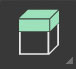
\includegraphics{Chapters/Images/Chapter_11/11_1_Icon_Extrude.png}

\caption{\label{fig-1_1}Extrude-Icon.}

\end{figure}%

\marginnote{Extrusion verbindet Elemente direkt}

Beim Extrudieren von Elementen werden diese Elemente nicht nur
dupliziert, sondern auch automatisch mit den originalen Elementen
verbunden. Wird bei der Auswahl eines Faces die Taste gedrückt, wird
dieses Face von der originalen Position gelöst und kann verschoben
werden. Gleichzeitig ist es allerdings über weitere Faces noch mit den
Vertices des originalen Faces verbunden. Beim Extrudieren werden also
die ausgewählten Elemente aus dem Objekt herausgezogen, ohne die
originalen Vertices zu löschen.

\marginnote{Beim Extrudieren erzeugte Elemente}

Nebst Faces lassen sich auch Vertices und Edges extrudieren. Wenn ein
einzelner Vertex extrudiert wird, generiert Blender automatisch ein Edge
zwischen dem originalen Vertex und dem extrudierten Vertex. Wenn ein
Edge extrudiert wird, generiert Blender automatisch ein Face zwischen
dem originalen Edge und dem neuen Edge. Wird ein Face extrudiert, werden
automatisch Faces zwischen den originalen Vertices/Edges und den neuen
Vertices/Edges erstellt.

\marginnote{Extrudieren präzisieren}

Wie auch bei Transformationen kann die Extrusion mittels der Tasten
\kbd{X}, \kbd{Y} oder \kbd{Z} auf einzelne Achsen beschränkt werden und
mittels der Angabe von Zahlen angegeben werden, wie gross die Distanz
zum originalen Median der Auswahl sein soll. Zudem kann das Extrudieren
auch mittels der Taste \kbd{S} mit einer Skalierung verbunden werden.

\marginnote{Faces werden per Default entlang Normalen extrudiert}

Beim Extrudieren von Faces erfolgt die Bearbeitung per Default entlang
der Normalen des Faces. Dadurch wird automatisch entlang der Ausrichtung
der Faces extrudiert. Dies ist bei Vertices und Edges nicht der Fall.

Übung 6: Extrudieren

\textbf{Übung 6.1}

Erstellen Sie folgende Objekte ausgehend von einem Würfel.

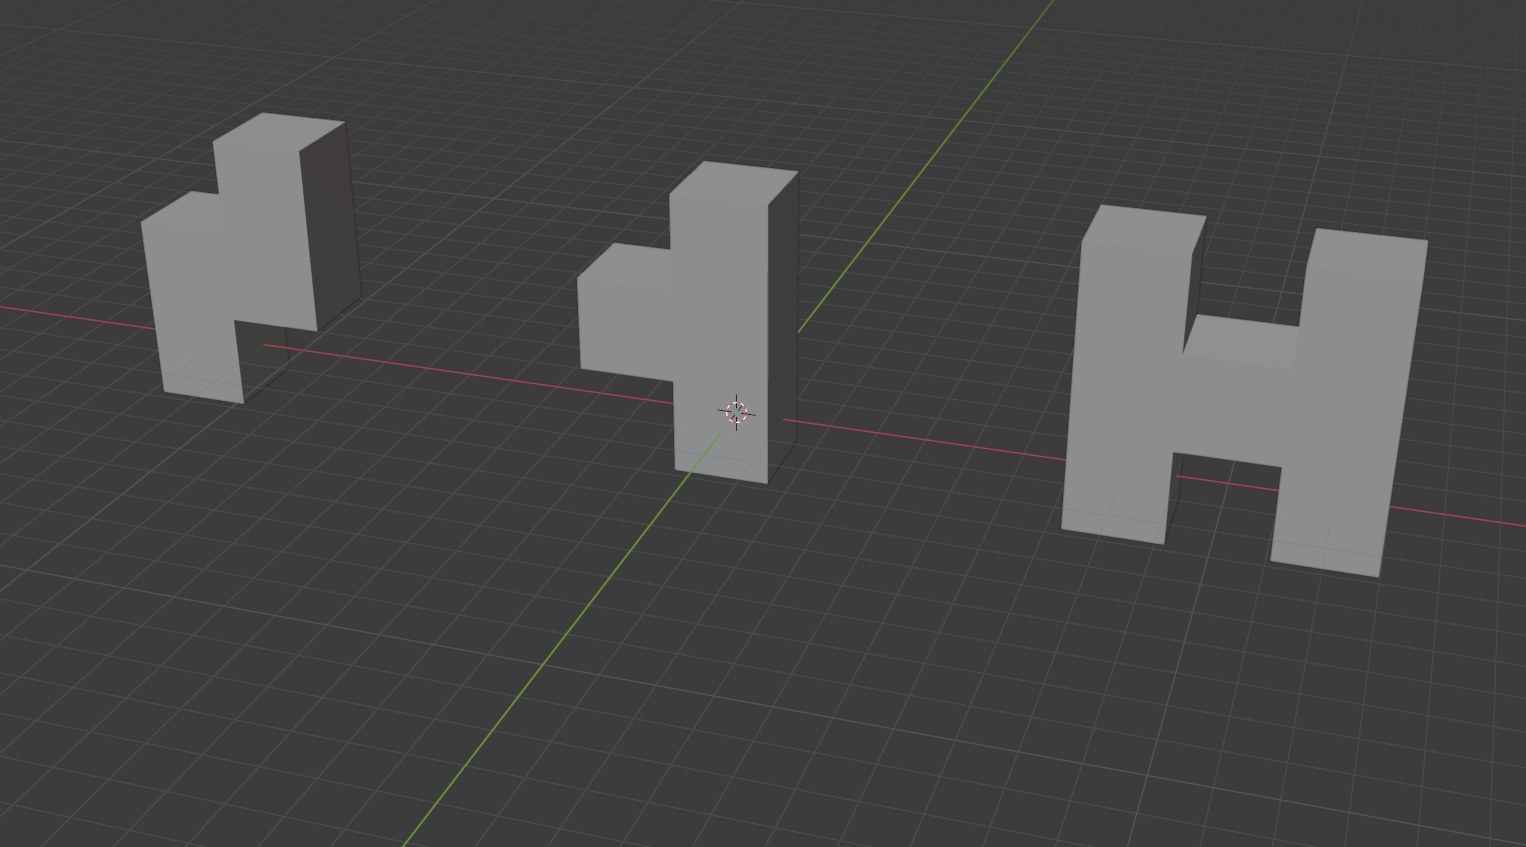
\includegraphics{Chapters/Images/Chapter_11/Exercise_6_1.png}\hfill

\section{Knife}\label{knife}

\marginnote{Schneiden mittels \kbd{K}}

Es ist möglich, Faces und Edges mittels des Befehls «Knife» zu
zerschneiden. Dadurch resultieren neue Vertices und Edges innerhalb von
Flächen und Kanten. Diese Operation lässt sich ebenfalls in der Toolbar
auswählen. Allerdings ist es auch möglich, mittels der Taste \kbd{K}
diese Operation direkt auf der Tastatur anzuwählen.

\begin{figure}

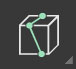
\includegraphics{Chapters/Images/Chapter_11/11_2_Icon_Knife.png}

\caption{\label{fig-1_2}Knife-Icon.}

\end{figure}%

\marginnote{Ansicht im Schnitt-Modus}

Sobald das Knife-Werkzeug über die Toolbar oder die Taste \kbd{K}
aktiviert wird, verwandelt sich der Mauszeiger in ein Messer. Wird die
Maus nun über das Objekt bewegt, wird mittels eines grünen Vierecks
angezeigt, an welcher Stelle am Objekt gerade geschnitten werden kann.
Befindet sich an dieser Stelle zudem ein Vertex, wird dies durch eine
rote Umrandung des grünen Vierecks signalisiert. Befindet sich das grüne
Viereck an einem Edge, wird dieses Edge grün markiert.

\marginnote{Schnitte setzen}

Um Schnitte zu platzieren, wird die linke Maustaste gedrückt. Die
Schnittpositionen werden anhand eines Vierecks markiert und weitere
Schnitte können ebenfalls mit der linken Maustaste an der entsprechenden
Position gesetzt werden. Dabei werden automatisch Edges zwischen den
einzelnen Schnittpunkten erzeugt. Passieren Schnittpunkte ein Edge, wird
an der Schnittstelle des Edges zudem automatisch ein Vertex erzeugt.

\marginnote{Schnitte bestätigen oder abbrechen}

Mittels der Taste \kbd{Space} oder \kbd{Enter} wird der Schneidevorgang
bestätigt. Dadurch wird der Schneidmodus verlassen und die
entsprechenden Vertices und Edges werden gesetzt. Um den Schneideprozess
abzubrechen, kann die rechte Maustaste oder \kbd{esc}-Taste gedrückt
werden.

\section{Loop Cut}\label{loop-cut}

\marginnote{Prinzip des Loop Cuts}

Das Messer-Werkzeug ist nützlich, um kreativ und flexibel Schnitte zu
erzeugen. Oftmals werden allerdings gerade Schnitte entlang einer ganzen
Fläche benötigt, idealerweise auch in der Mitte der Fläche. Hierfür ist
das Loop-Cut-Werkzeug geeignet. Nebst der exakten Mitte können auch
andere Schnitteinheiten exakt berücksichtig werden, beispielsweise dass
ein Bereich exakt nach einem Zehntel der Länge geschnitten werden soll.

\begin{figure}

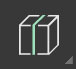
\includegraphics{Chapters/Images/Chapter_11/11_3_Icon_LoopCut.png}

\caption{\label{fig-1_3}Loop-Cut-Icon.}

\end{figure}%

\marginnote{Loop Cut mittels \kbd{Ctrl} + \kbd{R}}

Das Loop-Cut-Tool kann entweder in der Toolbar oder mittels der
Tastenkombination \kbd{Ctrl} + \kbd{R} aktiviert werden. Wird
anschliessend der Mauszeiger über die Oberfläche des Objekts bewegt,
werden Vorschläge dargestellt, wie das Objekt gerade durchtrennt werden
kann. Dabei werden aneinandergrenzende Faces als Loop berücksichtig,
sodass sie durchtrennt werden können.

\marginnote{Mehrere Schnitte im Loop Cut setzen}

Es können auch mehrere parallele Schnitte gemacht werden. Hierfür wird
die Anzahl Schnitte als Zahl über die Tastatur eingegeben. So kann etwa
der Standardwürfel entlang einer Flächenreihe in vier gleich grosse
Flächen unterteilt werden, indem die Taste \kbd{3} gedrückt wird.
Dadurch werden drei Linien angezeigt, welche den Bereich in vier gleich
grosse Teile unterteilen.

\marginnote{Loop Cut bestätigen oder abbrechen}

Durch einen Klick mit der linken Maustaste oder \kbd{Enter}-Taste wird
bestätigt, dass das Objekt entlang der dargestellten Linie zerschnitten
werden soll. Um den Schneideprozess abzubrechen, kann die rechte
Maustaste, \kbd{Delete} oder \kbd{esc} gedrückt werden.

\marginnote{Loop Cut justieren}

Wenn die Auswahl der Linie bestätigt wird, kann anschliessend noch
justiert werden, in welchem Bereich der Schnitt gemacht werden soll. Per
Default liegt der Schnitt genau in der Mitte. Mittels einer Bewegung mit
dem Mauszeiger kann der Schnitt entlang des Loops verschoben werden.
Alternativ kann auch mittels einer Zahleneingabe über die Tastatur
definiert werden, in welchem Bereich der Schnitt erfolgen soll. Mit
einem Wert von 0.5 wird ein einzelner Schnitt prozentual um die Hälfte
in die eine Richtung verschoben, mit einem Wert von -0.5 um die Hälfte
in die andere Richtung. Durch einen Klick mit der linken Maustaste oder
\kbd{Enter}-Taste wird die Linie bestätigt und die Schnitte werden
gesetzt. Durch das Drücken der \kbd{Delete}- oder \kbd{esc}-Taste wird
der Schnitt in der Mitte des Loops vollzogen.

\begin{tipp}{Weiterführende Informationen}
Der Loop Cut kann auch auf Edges angewendet werden, die noch nicht Teil eines Faces sind. Dabei wird das Edge genau in der Mitte durch einen Vertex in zwei Edges unterteilt.
\end{tipp}

\section{Edge Slide}\label{edge-slide}

\marginnote{Edge Slide}

Der Loop Cut beinhaltet somit zwei Schritte: Die Festlegung eines
Schnittes innerhalb eines Loops und zusätzlich die Festlegung, in
welchem Bereich des Face-Loops der Cut erfolgen soll. Letzterer Prozess
kann bei der Auswahl eines Loops an bereits gesetzten Edges direkt
erfolgen. Dieser Prozess wird als Edge Slide bezeichnet und ist in der
Toolbar verfügbar. Dadurch lässt sich eine Reihe von Edges proportional
entlang anderer Edges verschieben.

\begin{figure}

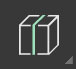
\includegraphics{Chapters/Images/Chapter_11/11_3_Icon_LoopCut.png}

\caption{\label{fig-1_4}Edge-Slide-Icon.}

\end{figure}%

\section{Subdivide}\label{subdivide}

\marginnote{Unterteilung mittels Loop Cut}

Dank des Loop Cuts ist es möglich, dass der Standardwürfel in gleich
grosse Unterwürfel unterteilt wird. Hierfür muss lediglich auf alle drei
Loops -- also entlang der X-, Y- und Z-Achse -- des Würfels ein Cut
angewendet werden. Anschliessend ist jede Seite des Würfels in vier
Faces unterteilt.

\marginnote{Subdivision, um Objekte zu unterteilen}

Statt alle drei Loop Cuts einzeln zu erstellen, kann der Würfel mittels
des Befehls «\emph{Subdivide}» unterteilt werden. Dieser ist über das
Menü «\emph{Edge \textbar{} Subdivide}» verfügbar. Anschliessend werden
alle ausgewählten Faces entlang zweier Achsen unterteilt, sodass sie aus
vier einzelnen Faces bestehen. Diese Aktion kann auch auf Edges
angewendet werden, die nicht Teil eines Faces sind. Im Kontext-Menü zur
letzten durchgeführten Aktion kann zudem die Anzahl Unterteilungen
erhöht werden.

\section{Bevel}\label{bevel}

\marginnote{Abrunden mittels \kbd{Ctrl} + \kbd{B}}

Mithilfe der Bevel-Transformation können Kanten abgerundet werden.
Hierfür wird das entsprechende Edge durch mehrere Edges ersetzt, sodass
eine Abrundung der Kante erfolgt. Der Befehl für das Abschrägen kann
über die Toolbar erfolgen oder mittels der Tastenkombination \kbd{Ctrl}
+ \kbd{B}.

\begin{figure}

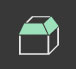
\includegraphics{Chapters/Images/Chapter_11/11_5_Icon_Bevel.png}

\caption{\label{fig-1_5}Bevel-Icon.}

\end{figure}%

\marginnote{Abrundung durchführen}

Um eine Kante abrunden zu können, muss das entsprechende Edge zunächst
ausgewählt werden. Nach der Auswahl kann die Bearbeitung mit der
Tastenkombination \kbd{Ctrl} + \kbd{B} gestartet werden. Dadurch
erscheint am Mauszeiger ein Faden, welcher zum Median der Auswahl führt.
Durch das Bewegen des Mauszeigers vom Median weg werden die ausgewählten
Edges in je zwei Edges aufgeteilt, die sich von den originalen Edges
wegentfernen und dabei eine Abrundung bilden. Durch einen Klick mit der
linken Maustaste oder \kbd{Enter}-Taste wird die Abrundung zu einer
bestimmten Position bestätigt. Durch das Drücken der rechten Maustaste,
\kbd{Delete}- oder \kbd{esc}-Taste wird der Vorgang abgebrochen.

\marginnote{Abrundung verfeinern}

Im Kontext-Menü zur letzten durchgeführten Aktion sind weitere Optionen
zur Abrundung möglich. So können die Anzahl Segmente, mit der die
Abrundung erfolgt, noch erhöht werden. Je mehr Segmente, desto glatter
wirkt die Abrundung. Zudem kann die Form anhand des Faktors für die
«\emph{Shape}» bearbeitet werden. Je näher dieser Faktor gegen 0 strebt,
desto mehr erfolgt die Abrundung hin zum Inneren des Objektes, und je
näher der Faktor gegen 1 strebt, desto mehr erfolgt die Abrundung hin
zum Äusseren des Objektes.

\marginnote{Vertices abrunden}

Die Bevel-Transformation kann sowohl für Edges als auch für Vertices
angewendet werden. Hierfür muss im Kontext-Menü zur letzten
durchgeführten Aktion eingestellt werden, dass die Vertices bearbeitet
werden anstelle der Edges. Hierfür werden unter der Zeile
«\emph{Affect}» die Vertices ausgewählt. Dadurch lassen sich Ecken
abrunden. Durch die Auswahl von Edges bei der Zeile «\emph{Affect}»
werden die Kanten abgerundet.

\section{Inset Faces}\label{inset-faces}

\marginnote{Intrusion mittels \kbd{I}}

Die Transformation «Inset Faces» stellt einen Spezialfall der Extrusion
dar. Dabei wird eine Fläche unterteilt in zusätzliche Flächen innerhalb
dieser Fläche. Wie auch bei der Extrusion werden dabei neue Vertices
erstellt, welche direkt an den originalen Vertices andocken.
Unterschiedlich ist allerdings, dass die neuen Vertices einen Teil der
originalen Faces darstellen und somit entlang der Ausrichtung der Fläche
vergrössert oder verkleinert werden können. Die Bearbeitung mittels
Inset Faces kann entweder über die Toolbar oder mittels der Taste
\kbd{I} erfolgen.

\begin{figure}

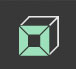
\includegraphics{Chapters/Images/Chapter_11/11_6_Icon_Inset_Faces.png}

\caption{\label{fig-1_6}Inset-Faces-Icon.}

\end{figure}%

\marginnote{Intrusion durchführen}

Um die Bearbeitung zu starten, muss mindestens ein Face ausgewählt
werden und die Taste \kbd{I} gedrückt werden. Wie auch beim Skalieren
von Elementen ist der Mauszeiger nun mittels eines Fadens zum Median der
Auswahl verbunden. Wenn die Maus näher zum Median hin bewegt wird,
erscheinen zusätzliche Faces innerhalb der Auswahl, die jeweils kleiner
werden, je näher der Mauszeiger dem Median kommt.

\marginnote{Dicke der Intrusion}

Die Intrusion wird anhand der Breite der neu erstellten Faces
beschrieben. Wird beispielsweise nach dem Drücken der Taste \kbd{I} die
Taste \kbd{1} gedrückt, sind die neuen Faces jeweils um einen Meter von
ihren ursprünglichen Edges entfernt. Durch zu hohe Zahlen kann dies dazu
führen, dass sich die Faces kreuzen.

\marginnote{Individuelle Intrusion}

Die Funktion Inset Faces kann zudem auf die Faces individuell angewendet
werden. Im Normallfall werden zwei nebeneinander ausgewählte Faces
gemeinsam bearbeitet. Es ist jedoch auch möglich, die Faces individuell
anzusteuern, sodass die ausgewählten Faces individuell bearbeitet
werden. Hierfür muss im Kontext-Menü zur letzten durchgeführten Aktion
die Option «\emph{Individual}» angewählt werden.

\section{Spin}\label{spin}

\marginnote{Spin}

Mittels «Spin» können einzelne oder mehrere Vertices in einer
kreisförmigen Anordnung extrudiert werden. Wenn diese Transformation
ausgewählt ist, erscheint in der Nähe des 3D-Cursors ein Gizmo, welches
eine abgerundete Linie mit einem Plus-Symbol an beiden Enden darstellt.
Falls dieses Gizmo nicht angezeigt wird, sollte überprüft werden, ob die
Darstellung der Gizmos im 3D-Viewport aktiviert ist.

\begin{figure}


\includegraphics{Chapters/Images/Chapter_11/11_7_Icon_Spin.png}

\caption{\label{fig-1_7}Spin-Icon.}

\end{figure}%

\marginnote{Spin durchführen}

Um Vertices nun kreisförmig zu extrudieren, müssen Sie zunächst
ausgewählt werden. Anschliessend kann an einem der beiden Pluszeichen
gezogen werden und die Vertices werden kreisförmig um den 3D-Cursor
herum extrudiert. Dabei werden per Default zwölf Vertices erstellt --
unabhängig davon, wie weit im Kreis extrudiert wird.

\marginnote{Spin verfeinern}

Im Kontext-Menü zur letzten durchgeführten Aktion kann die Aktion noch
bearbeitet werden, sodass etwa die Anzahl extrudierter Vertices unter
«\emph{Steps}» verändert werden kann. Je mehr Vertices extrudiert
werden, desto glatter wirkt der Kreis. Unter «\emph{Angle}» kann mittels
einer Winkelangabe eingestellt werden, wie weit die Extrusion um den
3D-Cursor herum erfolgen soll. Wenn die Zeile «\emph{Auto Merge}»
aktiviert ist, werden Vertices an derselben Position -- beispielsweise
die Vertices am Anfang und Ende einer 360°-Umdrehung -- zu einem Vertex
kombiniert.

\section{Merge}\label{merge}

\marginnote{Verbinden mittels \kbd{M}}

In den bisherigen Transformationen wurden jeweils neue Vertices, Edges
oder Faces hinzugefügt. Manchmal kommt es vor, dass einige Elemente
wieder entfernt werden müssen, oder dass sie an einer Stelle verbunden
werden müssen. Hierfür kann der Befehl «\emph{Merge}» verwendet werden.
Dieser lässt sich mittels der Taste \kbd{M} innerhalb eines Menüs beim
Mauszeiger auswählen.

\marginnote{Elemente beim Median verbinden}

Wenn beispielsweise zwei Vertices ausgewählt werden und die Taste
\kbd{M} gedrückt wird, können die Vertices durch «\emph{At Center}» beim
Median zwischen den beiden Vertices verbunden werden. Dabei werden die
beiden Vertices zusammengeführt zu einem Vertex, welches alle Edges und
Faces der originalen Vertices aufnimmt. Das Mergen kann zudem mit
beliebig vielen Vertices vollzogen werden. Bei der Auswahl von Edges und
Faces werden dabei die beteiligten Vertices zur Zusammenführung
verwendet.

\marginnote{Andere Verbindungspunkte}

Nebst dem Medianpunkt der Vertices können auch folgende Positionen zur
Zusammenführung ausgewählt werden:

\begin{itemize}
\tightlist
\item
  \textbf{At Cursor}: Die Vertices werden an der Position des 3D-Cursors
  zusammengeführt.
\item
  \textbf{At First}: Die Vertices werden beim Vertex, welcher als Erstes
  ausgewählt wurde, zusammengeführt.
\item
  \textbf{At Last}: Die Vertices werden beim Vertex, welcher als Letztes
  ausgewählt wurde, zusammengeführt.
\item
  \textbf{Collapse}: Wenn mehrere Edges ausgewählt werden, die nicht
  miteinander verbunden sind, werden die Vertices jeweils in der Mitte
  des jeweiligen Edges zusammengeführt. Das Zusammenführen erfolgt also
  hierbei einzeln für jedes Edge in dessen Mitte (bei den anderen
  Optionen werden alle Vertices an demselben Punkt zusammengeführt).
\end{itemize}

\marginnote{Merge by Distance}

Eine besondere Rolle kommt der Funktion «\emph{Merge by Distance}» zu.
Dabei werden alle Vertices zusammen verbunden, deren Distanz geringer
als die vorgegebene Distanz ist. Im Kontext-Menü zur letzten Aktion
lässt sich die Distanz, unterhalb derer alle Vertices verbunden werden
sollen, anpassen. Die Funktion wird allerdings nur auf die ausgewählten
Vertices angewendet. In der Fussleiste von Blender wird temporär
angegeben, wie viele Vertices bei dieser Aktion aufgelöst werden.

\marginnote{Merge erfolgt nur auf Auswahl}

Diese Methode ist besonders geeignet, um allfällige Vertices, welche an
derselben Position wie andere Vertices liegen, zu eliminieren oder zu
verbinden. Da die Aktion allerdings nur auf ausgewählte Vertices
angewendet wird, empfiehlt es sich, vorgängig alle Vertices direkt mit
der Taste \kbd{A} auszuwählen.

\section{Weitere Operationen in der
Toolbar}\label{weitere-operationen-in-der-toolbar}

Nebst den bisher behandelten Operationen zur Objektbearbeitung im
Edit-Mode bietet die Toolbar noch eine Reihe weiterer Optionen, welche
der Vollständigkeit halber noch kurz aufgeführt werden.

\subsection{Add Cube}\label{add-cube}

\marginnote{Würfel hinzufügen}

Mittels des Befehls «\emph{Add Cube}» kann ein neuer Würfel erstellt
werden. Um den Maus zeiger herum erscheint dadurch ein Gitternetz, um zu
signalisieren, wo der Würfel erstellt wird. Anschliessend kann mittels
gedrückter linken Maustaste der Grundriss des Würfels erstellt werden.
Nachdem die linke Maustaste losgelassen wurde, lässt sich anschliessend
noch die Höhe des Würfels einstellen, welche anschliessend mit bestätigt
werden muss. Mit \kbd{esc} oder die rechte Maustaste lässt sich der
Vorgang abbrechen.

\begin{figure}

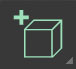
\includegraphics{Chapters/Images/Chapter_11/11_8_Icon_AddCube.png}

\caption{\label{fig-1_8}Add-Cube-Icon.}

\end{figure}%

Die neu erstellten Würfel werden im Edit-Mode zu Bestandteilen des
Objekts, welches gerade bearbeitet wird. Der Befehl «\emph{Add Cube}»
steht allerdings auch im Object-Mode zur Verfügung. Werden dort neue
Würfel erstellt, bilden diese jeweils eigenständige Objekte.

\subsection{Poly Build}\label{poly-build}

\marginnote{Poly-Build-Modus}

Beim Poly Build handelt es sich um einen interaktiven Modus, um
Geometrien zu erweitern. Dabei schlägt Blender bei gedrückter
\kbd{Ctrl}-Taste vor, wie neue Elemente erstellt werden können, und
durch einen Klick mittels der linken Maustaste wird die Erstellung
bestätigt. Mittels gedrückter linken Maustaste können Vertices bewegt
werden und mittels der Kombination \kbd{Shift} + linke Maustaste.

\begin{figure}

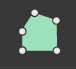
\includegraphics{Chapters/Images/Chapter_11/11_9_Icon_PolyBuild.png}

\caption{\label{fig-1_9}Poly-Build-Icon.}

\end{figure}%

\subsection{Smooth}\label{smooth}

\marginnote{Objekte glätten}

Mittels des Befehls «Smooth» können Objekte glatter gemacht werden. Dies
geschieht, indem die Winkel der Edges gemittelt werden. Statt eines
90°-Winkels entsteht dann ein flacherer Winkel. Es ist allerdings auch
möglich, den gegenteiligen Effekt zu erzielen und Winkel spitzer zu
machen.

\begin{figure}

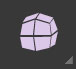
\includegraphics{Chapters/Images/Chapter_11/11_10_Icon_Smooth.png}

\caption{\label{fig-1_10}Smooth-Icon.}

\end{figure}%

\subsection{Shrink/Fatten}\label{shrinkfatten}

\marginnote{Objekte zusammenziehen oder aufblähen}

Beim Befehl «Shrink/Fatten» werden die ausgewählten Vertices entlang
ihrer eigenen Normalen bewegt. Dadurch kann das Objekt aufgebläht oder
zusammengezogen werden. Dies ist beispielsweise nützlich, wenn der
Mantel eines Zylinders ausgewählt und sein Radius vergrössert werden
soll, ohne dessen Höhe zu verändern.

\begin{figure}

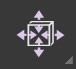
\includegraphics{Chapters/Images/Chapter_11/11_11_Icon_ShrinkenFatten.png}

\caption{\label{fig-1_11}Shrink/Fatten-Icon.}

\end{figure}%

\subsection{Shear}\label{shear}

\marginnote{Objekte auseinanderziehen}

Mittels der Shear-Transformation werden die ausgewählten Punkte in einer
Achse aus einandergezogen. Die Transformation geschieht dabei so, dass
parallel verlaufende Linien geschert und in entgegengesetzte Richtungen
auf einer Achse verschoben werden.

\begin{figure}

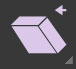
\includegraphics{Chapters/Images/Chapter_11/11_12_Icon_Shear.png}

\caption{\label{fig-1_12}Shear-Icon.}

\end{figure}%

\subsection{Rip Region}\label{rip-region}

\marginnote{Regionen aufteilen}

Mittels des Befehls «Rip Region» können Vertices, welche an mehreren
Faces andocken, aufgeteilt werden. Die Faces werden dabei an der Stelle
der entsprechenden Vertices getrennt und durch Vertices, welche
sozusagen von den originalen Vertices abgezogen werden, neu gebildet.

\begin{figure}

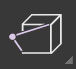
\includegraphics{Chapters/Images/Chapter_11/11_13_Icon_RipRegion.png}

\caption{\label{fig-1_13}Rip-Region-Icon.}

\end{figure}%

Übung 7: Objektbearbeitung

\textbf{Übung 7.1}

Verändern Sie den Standardwürfel im Edit-Mode so, dass er die Form eines
Hauses hat.

\textbf{Übung 7.2}

Erstellen Sie eine Vase. Die Vase sollte rund sein und eine Öffnung
haben -- ansonsten sind Sie frei in Ihrer Gestaltung. Achten Sie zudem
darauf, dass Sie unterschiedliche Faces für den Innenbereich und für den
Aussenbereich der Vase verwenden, sodass die Vase ein gewisse Dicke
besitzt.

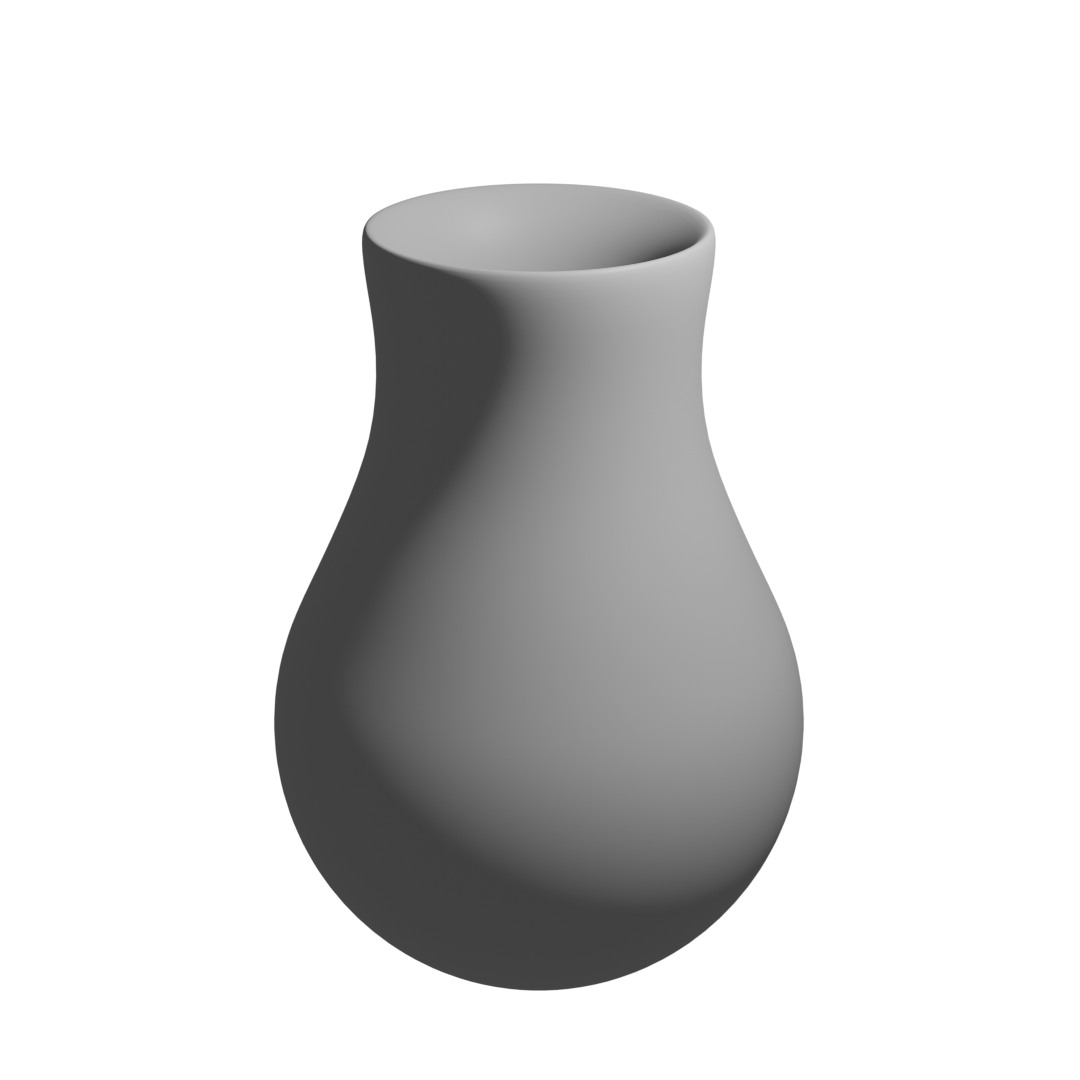
\includegraphics{Chapters/Images/Chapter_11/Exercise_7_2.png}\hfill

\chapter{Hilfestellungen für die
Objektbearbeitung}\label{hilfestellungen-fuxfcr-die-objektbearbeitung}

Blender bietet eine Reihe von Hilfestellungen, welche nützlich für die
Erstellung von 3D-Objekten sind. Einige dieser Hilfestellungen sind im
Header des 3D-Viewports aufzufinden.

\section{Die Position des 3D-Cursors
verändern}\label{die-position-des-3d-cursors-veruxe4ndern}

\marginnote{3D-Cursor verschieben und rotieren}

Der 3D-Cursor wird für einige der Hilfsmittel benötigt. Deshalb ist es
sinnvoll, sich damit zu befassen, wie der 3D-Cursor bewegt werden kann.
In der Sidebar, welche mit der Taste \kbd{N} ein- und ausgeblendet
werden kann, befindet sich unter dem Register «\emph{View}» ein
Abschnitt zum 3D-Cursor. An dieser Stelle kann die Position des Cursors
im dreidimensionalen Raum anhand der X-, Y- und Z-Achse definiert
werden. Nebst der Position verfügt der 3D-Cursor über eine Rotation,
welche ebenfalls an dieser Stelle definiert werden kann. Durch eine
Veränderung der Rotation des 3D-Cursors verändert sich auch die Rotation
der Linien, welche den 3D-Cursor im 3D-Viewport kreuzen. Diese Linien
stellen die Rotation des 3D-Cursors dar.

\begin{figure}

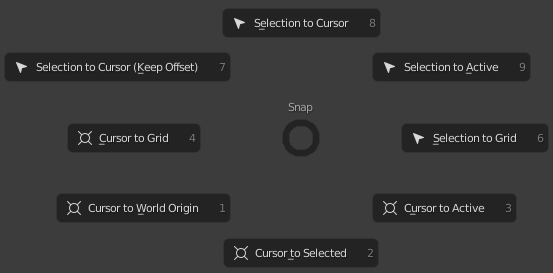
\includegraphics{Chapters/Images/Chapter_12/12_1_Snap_Menu.png}

\caption{\label{fig-1_1}Snap-Menü.}

\end{figure}%

\marginnote{Snap-Menü}

Mittels der Tastenkombination \kbd{Shift} + \kbd{S} lässt sich das
sogenannte «\emph{Snap}»-Menü öffnen. Dieses sich erscheint direkt beim
Mauszeiger und ermöglicht es, ausgewählte Objekte oder den 3D-Cursor an
bestimmte Positionen zu verschieben. Das Menü beinhaltet folgende
Optionen:

\begin{itemize}
\tightlist
\item
  \textbf{Cursor to Grid}: Dadurch wird der 3D-Cursor an die
  nächstliegende Position des Koordinatengitters verschoben, welches als
  Viewport-Overlay angezeigt wird.
\item
  \textbf{Cursor to World Origin}: Dadurch wird der 3D-Cursor an den
  Ursprung der Welt positioniert. Dies entspricht dem Nullpunkt aller
  drei Achsen.
\item
  \textbf{Cursor to Selected}: Der 3D-Cursor wird an der Position des
  ausgewählten Objektes respektive dem Median der aktuellen Auswahl
  positioniert.
\item
  \textbf{Cursor to Active}: Der 3D-Cursor wird an der Position des
  aktiven Elementes positioniert.
\item
  \textbf{Selection to Cursor (Keep Offset)}: Alle ausgewählten Elemente
  werden zum 3D-Cursor verschoben, sodass sich der Median der
  ausgewählten Elemente an der Position des 3D-Cursors befindet. Die
  Relationen zwischen den ausgewählten Objekten bleiben dabei bestehen.
\item
  \textbf{Selection to Cursor}: Alle ausgewählten Elemente werden zum
  3D-Cursor verschoben, sodass sich die Position jedes individuellen
  Elementes an der Position des 3D-Cursors befindet. Im Edit Mode führt
  dies dazu, dass alle ausgewählten Vertices auf der Position des
  3D-Cursors liegen.
\item
  \textbf{Selection to Active}: Die Auswahl wird an die Position des
  aktiven Objektes verschoben. Im Edit Mode führt dies dazu, dass alle
  ausgewählten Vertices auf derselben Position liegen.
\item
  \textbf{Selection to Grid}: Das ausgewählte Element oder der Median
  der ausgewählten Elemente wird an die nächstliegende Position des
  Koordinatengitters verschoben, welches als Viewport-Overlay angezeigt
  wird. Im Edit-Mode werden die ausgewählten Elemente ebenfalls an die
  nächstliegende Position des Koordinatengitters verschoben. Wenn die
  Ansicht jedoch zu weit hinausgezoomt wird und die Elemente dadurch
  visuell an derselben Stelle zu sein scheinen, werden alle ausgewählten
  Vertices dabei an derselben Position platziert.
\end{itemize}

\section{Transform Orientation}\label{transform-orientation}

\marginnote{Verschiedene Orientierungen für Transformationen}

Bei Transformationen können die X-, Y- und Z-Achsen zu Hilfe genommen
werden. Diese Achsen scheinen fix festgelegt zu sein. Es gibt allerdings
verschiedene Orientierungen für diese Achsen. Die Transform-Orientation
beschreibt diese Orientierung der Achsen. Es stehen folgende
Orientierungen zur Verfügung:

\begin{itemize}
\tightlist
\item
  Global
\item
  Local
\item
  Normal
\item
  Gimbal
\item
  View
\item
  Cursor
\end{itemize}

\begin{figure}

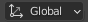
\includegraphics{Chapters/Images/Chapter_12/12_2_Transform_orientation.png}

\caption{\label{fig-1_2}Auswahl der Transform-Orientation.}

\end{figure}%

\marginnote{Gizmos helfen bei der Orientierung}

Um ein besseres Verständnis für die Unterschiede in den
Transform-Orientierungen zu bekommen, ist es sinnvoll, unter dem
Dropdown-Menü für die Viewport-Gizmos das Gizmo für die Bewegung
einzuschalten. Dadurch erscheint ein Gizmo, welches vorgibt, in welche
Richtung die Achsen durch die Transform-Orientierung verlaufen.

\subsection{Global}\label{global}

\marginnote{Globale Orientierung}

Die globale Orientierung entspricht immer genau den Achsen der Welt. Das
heisst, man kann sich dabei immer an den vorgegebenen Achsen im
Viewport-Overlay orientieren.

\subsection{Local}\label{local}

\marginnote{Lokale Orientierung}

Die lokale Orientierung entspricht jeweils der Orientierung eines
Objektes. Wenn ein Objekt im Object-Mode um 20° rotiert wurde, sind auch
die Achsen um diese 20° rotiert. Dies Einstellung gilt sowohl für den
Object- als auch für den Edit-Mode. Im Object-Mode unterscheiden sich
die Gizmos zwischen den verschiedenen Objekten, je nach deren Rotation.

\subsection{Normal}\label{normal}

\marginnote{Orientierung entlang der Normalen}

Die Orientierung anhand der Normalen verläuft im Edit-Mode so, dass die
Z-Achse immer den Normalen der ausgewählten Einheiten entspricht. Die X-
und Y-Achse beschreiben dann die Achsen im Verhältnis zu den Normalen.
Wenn mehrere Elemente ausgewählt sind, entspricht die Z-Achse dem
Mittelwert der Normalen. Im Object-Mode ist diese Orientierung
äquivalent zur lokalen Orientierung.

\begin{tipp}{Weiterführende Informationen}
Beim Extrudieren mittels \kbd{E} schlägt Blender eine Extrusion entlang der Z-Achse in der Normal-Orientierung vor. Deshalb muss jeweils zweimal die Taste \kbd{Z}gedrückt werden, um entlang der globalen Z-Achse zu extrudieren – einmal, um die Z-Achse entlang der Normal-Orientierung abzuwählen, und einmal, um die Z-Achse entlang der eingestellten Orientierung auszuwählen.
\end{tipp}

\subsection{Gimbal}\label{gimbal}

\marginnote{Gimbal-Orientierung}

Die Gimbal-Orientierung stellt eine fortgeschrittene
Orientierungsmethode dar, welche bei Euler-Rotationen von Nutzen sein
kann. Im Rahmen dieses Kurses werden Euler-Rotationen nicht behandelt,
weshalb nicht weiter auf diese Orientierung eingegangen wird.

\subsection{View}\label{view}

\marginnote{Orientierung entlang der Ansicht}

Die View-Orientierung entspricht der Orientierung entsprechend der
Ansicht auf dem Bildschirm. Die X-Achse verläuft horizontal über den
Bildschirm und die Y-Achse vertikal. Die Z-Achse beschreibt die Achse
der eigenen Ansicht nach näher oder weiter weg.

\subsection{Cursor}\label{cursor}

\marginnote{Orientierung entsprechend dem 3D-Cursor}

Die 3D-Cursor-Orientierung verläuft entlang des 3D-Cursors. Dabei wird
die Rotation des 3D-Cursors berücksichtig, sodass die Achsen
entsprechend der 3D-Cursor-Rotierung verlaufen.

\subsection{Custom}\label{custom}

\marginnote{Eigene Orientierung hinzufügen}

Mittels der Plus-Schaltfläche ist es möglich, eigene Orientierungen zu
erstellen. So kann die lokale Orientierung eines Objekts abgespeichert
werden, um sie bei Objekten, die eigentlich eine andere lokale
Orientierung aufweisen, ebenfalls verwenden zu können.

\section{Pivot Point}\label{pivot-point}

\marginnote{Verschiedene Drehpunkte}

Eine Reihe von Transformationen orientieren sich an einem bestimmten
Drehpunkt im dreidimensionalen Raum. Wenn vom Standardwürfel etwa zwei
gegenüberliegende Faces ausgewählt werden, orientiert sich eine
Skalierung der Faces anhand der Medianposition der Vertices. Mittels des
Menüreiters «\emph{Transform Pivot Point}» können auch andere Drehpunkte
ausgewählt werden. Die Optionen sind dabei:

\begin{itemize}
\tightlist
\item
  Bounding Box
\item
  Center
\item
  3D Cursor
\item
  Individual Origins
\item
  Median Point
\item
  Active Element
\end{itemize}

\begin{figure}


\includegraphics{Chapters/Images/Chapter_12/12_3_Icon_Pivot_Point.png}

\caption{\label{fig-1_3}Icon für den Pivot-Point in der Default-Auswahl
(Median-Point).}

\end{figure}%

\subsection{Bounding Box Center}\label{bounding-box-center}

\marginnote{Bounding Box Center als Drehpunkt}

Die Option «\emph{Bounding Box Center}» berechnet jeweils eine
dreidimensionale Box um die ausgewählten Einheiten, welche gerade so
gross ist, dass sich die gesamte Auswahl darin befindet. Der Mittelpunkt
dieser Box wird als Drehpunkt für Transformationen verwendet. Im
Object-Mode werden lediglich die Ursprünge von Objekten für die
Berechnung der Box verwendet, nicht die Meshes. Im Edit-Mode wird die
Box um alle ausgewählten Einheiten berechnet.

\subsection{3D Cursor}\label{d-cursor}

\marginnote{3D-Cursor als Drehpunkt}

Die Option «\emph{3D Cursor}» verwendet die Position des 3D-Cursors als
Drehpunkt für Transformationen. Der 3D-Cursor kann in seiner Position
verändert werden, wodurch sich jede beliebige Stelle im drei
dimensionalen Raum als Drehpunkt verwenden lässt. Ein Objekt, das sich
an einer anderen Stelle als der 3D-Cursor befindet, würde bei dieser
Einstellung um den 3D-Cursor rotiert.

\subsection{Individual Origins}\label{individual-origins}

\marginnote{Individual Origin als Drehpunkt}

Die Option «\emph{Individual Origins}» benutzt für jede ausgewählte
Einheit den individuellen Ursprung als Drehpunkt. Wenn im Object-Mode
mehrere Objekte ausgewählt sind, deren Ursprünge sich an verschiedenen
Positionen befinden, verwendet jedes Objekt seinen eigenen Ursprung als
Drehpunkt. Im Edit-Mode werden ausgewählte Einheiten, die nicht direkt
miteinander verbunden sind, als individuelle Einheiten betrachtet. Diese
verwenden den Median der Auswahl als Drehpunkt für Transformationen.
Werden vom Default-Cube beispielsweise zwei gegenüberliegende Faces
ausgewählt, wird von jedem Face individuell der Median berechnet und
dieser für das jeweilige Face als Drehpunkt verwendet. Wenn mehrere
Faces, die direkt nebeneinander liegen, ausgewählt sind, werden die
aneinanderliegenden Faces zusammengefasst und für diese gemeinsam ein
individueller Ursprung berechnet und als Drehpunkt verwendet.

\subsection{Median Point}\label{median-point}

\marginnote{Median als Drehpunkt}

Die Option «\emph{Median Point}» wird bei neuen Projekten als
Default-Auswahl für den Drehpunkt von Transformationen verwendet. Dabei
handelt es sich um die mittlere Position zwischen allen ausgewählten
Vertices im Edit-Mode. Wenn mehrere Objekte im Object-Mode ausgewählt
sind, wird der Median zwischen den Objekt-Ursprungspositionen als
Drehpunkt verwendet.

\subsection{Active Element}\label{active-element}

\marginnote{Ursprung des aktiven Elements als Drehpunkt}

Die Option «\emph{Active Element}» verwendet den Ursprung des aktiven
Elements als Drehpunkt für Transformationen. Beim aktiven Element
handelt es sich um das zuletzt ausgewählte Objekt, welches mit einer
orangen Umrandung gekennzeichnet ist. Der Ursprungspunkt dieses Objekts
wird als Drehpunkt für Transformationen verwendet. Im Edit-Mode ist das
aktive Element mit einer weissen Einfärbung markiert. Dieses Element,
respektive der entsprechende Median bei mehreren Edges, Faces oder
Vertices, wird anschliessend als Drehpunkt für Transformationen
verwendet.

\section{Snap}\label{snap}

\marginnote{Elemente an anderen Elementen andocken lassen}

Die Option «\emph{Snap}» ist bei der Verschiebung von Objekten nützlich.
Dadurch können andere Elemente benutzt werden, um die zu verschiebenden
Objekte direkt an deren Struktur andocken zu lassen. So müssen nicht die
etwaigen Koordinaten ermittelt werden, sondern Blender rastet die zu
bewegenden Objekte direkt an anderen Objekten ein. Die anvisierten
Strukturen können dabei im Edit-Mode Teil des eigenen Objektes sein,
aber auch Teil eines anderen Objektes. Im Object-Mode wird zudem jeweils
der Ursprung des Objektes zum Andocken verwendet. Im Dropdown-Menü kann
ein gestellt werden, an welchen Stellen jeweils angedockt werden soll:

\begin{itemize}
\tightlist
\item
  Increment
\item
  Vertex
\item
  Edge
\item
  Face
\item
  Volume
\item
  Edge Center
\item
  Edge Perpendicular
\end{itemize}

\begin{figure}


\includegraphics{Chapters/Images/Chapter_12/12_4_Icon_Snap.png}

\caption{\label{fig-1_4}Snap-Icon.}

\end{figure}%

\subsection{Increment}\label{increment}

\marginnote{Snap auf ein Inkrement}

Ist Snap auf «\emph{Increment}» eingestellt, so werden die Inkremente
der Welt verwendet, um Objekte anders zu platzieren. Mit diesen
Inkrementen sind die Gitterraster im Hintergrund der 3D-Ansicht gemeint.
Jedes Viereck stellt dabei ein Inkrement dar. Durch stärkeres Hinein-
oder Hinauszoomen im 3D-Viewport werden jeweils grössere oder kleinere
Inkremente sichtbar. Die ausgewählten Objekte rasten proportional
zueinander an der Stelle in einem Inkrement ein.

\subsection{Vertex}\label{vertex}

\marginnote{Snap auf Vertices}

Ist Snap auf «\emph{Vertex}» eingestellt, so können andere Vertices
angesteuert werden und Blender verbindet die Auswahl direkt auf der
entsprechenden Position. Dabei können auch die Vertices von anderen
Objekten angesteuert werden, selbst wenn diese nicht innerhalb des
Edit-Modes mitaktiviert wurden.

\subsection{Edge}\label{edge}

\marginnote{Snap auf Edges}

Ist Snap auf «\emph{Edge}» eingestellt, so können andere Edges als Ziel
angesteuert werden und die Auswahl wird direkt passend auf eine Position
auf dem Edge eingestellt. Dabei kann die ganze Länge eines Edges
ausgewählt werden. Es können zudem Edges von anderen Objekten
angesteuert werden, selbst wenn diese nicht innerhalb des Edit-Modes
aktiviert wurden.

\subsection{Face}\label{face}

\marginnote{Snap auf Faces}

Ist Snap auf «\emph{Face}» eingestellt, so versucht Blender, die Auswahl
direkt an der Position von anderen Faces anzudocken. Dabei kann jeder
Punkt auf einem Face ausgewählt werden. Zudem können auch hier die Faces
von anderen Objekten angesteuert werden.

\subsection{Volume}\label{volume-1}

\marginnote{Snap auf das Volumen}

Mittels der Einstellung von Snap auf «\emph{Volume}» lässt sich das
Volumen eines Objektes als genaues Ziel zum Einrasten einer Auswahl
verwenden. Oft ist nicht klar ersichtlich, wo genau das Objekt nun
einrastet, da das Volumen eines Objektes häufig durch die Faces verdeckt
wird. Hierbei kann die Wireframe-Ansicht helfen.

\subsection{Edge Center}\label{edge-center}

\marginnote{Snap auf die Mitte von Edges}

Mittels der Einstellung von Snap auf «\emph{Edge Center}» werden jeweils
die Mittelpunkte von Edges anvisiert. Hierbei werden also keine Vertices
anvisiert, sondern der Median des Edges. Andere Punkte auf dem Edge
werden nicht zum Einhaken angeboten.

\subsection{Edge Perpendicular}\label{edge-perpendicular}

\marginnote{Snap auf senkrechte Edges}

Mittels der Einstellung von Snap auf «\emph{Edge Perpendicular}» wird
die Auswahl bei dem Punkt eines Edges eingerastet, welcher im Lot zur
aktuellen Auswahl steht. Dabei können nicht alle Edges verwendet werden,
da nicht alle einen solchen Winkel zur Auswahl aufweisen.

\subsection{Was wird angedockt?}\label{was-wird-angedockt}

\marginnote{Quelle des Snaps einstellen}

Wenn lediglich ein einzelner Vertex ausgewählt und verschoben wird, ist
klar, welcher Punkt jeweils an den anvisierten Stellen andockt: der
ausgewählte Vertex. Wenn allerdings mehrere Elemente ausgewählt wurden,
benutzt Blender per Default das jeweils ursprünglich am nächsten
liegende Element zum Andocken. Es kann allerdings eingestellt werden,
dass der Median der aktivierten Auswahl oder das aktive Element
verwendet wird. Dies kann unter «\emph{Snap With}» eingestellt werden.
Zusätzlich gibt es noch die Auswahl «\emph{Center}», welche zusätzlich
noch weitere Abweichungen vom Drehpunkt mitberücksichtigt
(beispielsweise die ursprüngliche Abweichung vom 3D-Cursor).

\section{Proportional Editing}\label{proportional-editing}

\marginnote{Proportionale Bearbeitung mittels \kbd{O} aktivieren}

Die Option «\emph{Proportional Editing}» ermöglicht es, dass nahe
beieinanderliegende Elemente proportional zu ihrer Nähe bearbeitet
werden können. Diese Option kann auch mit der Taste \kbd{O} aktiviert
oder deaktiviert werden. Wenn diese Option aktiviert ist und eine
Transformation durchgeführt wird (z.B. eine Rotation), erscheint um den
Bezugspunkt ein Kreis. Alle Elemente, welche sich innerhalb dieses
Kreises befinden, werden diese Transformation nun ebenfalls durchführen.
Der Radius des Kreises kann mittels des Mausrads vergrössert oder
verkleinert werden. Dadurch wird der Erfassungsbereich der
proportionalen Bearbeitung variiert. Alternativ kann die Taste
\kbd{PageUp} zum Vergrössern des Kreises oder \kbd{PageDown} zum
Verkleinern des Kreises gedrückt werden..

\begin{figure}


\includegraphics{Chapters/Images/Chapter_12/12_5_Icon_Proportional_Editing.png}

\caption{\label{fig-1_5}Icon für Proportional Editing.}

\end{figure}%

\marginnote{Proportionale Bearbeitung im Object-Mode}

Im Object-Mode müssen jeweils die Ursprünge der Objekte, welche
proportional transformiert werden sollen, innerhalb des
Erfassungskreises liegen. Dabei spielt es keine Rolle, ob das Mesh des
Objektes ebenfalls erfasst wird oder nicht. Im Edit-Mode können
lediglich die Vertices der aktuell ausgewählten Objekte proportional
mittransformiert werden. Zudem gibt es im Edit-Mode die Möglichkeit, im
Dropdown-Menü des Proportional Editings die Option «\emph{Connected
Only}» anzuwählen. Dadurch werden lediglich Vertices bei der
proportionalen Bearbeitung berücksichtigt, die über Edges mit den zu
bearbeitenden Vertices verbunden sind.

\marginnote{Form der proportionalen Bearbeitung}

Die Elemente, welche sich innerhalb des Erfassungskreises befinden,
werden anschliessend alle proportional mittransformiert. Die Proportion
erfolgt dabei einer vorgegebenen Kurve, welche sich anhand des
Dropdown-Menüs genauer definieren lässt. Mithilfe der proportionalen
Bearbeitung lassen sich durch die Bearbeitung eines einzigen Vertex
komplexe Strukturen erstellen.

\begin{figure}

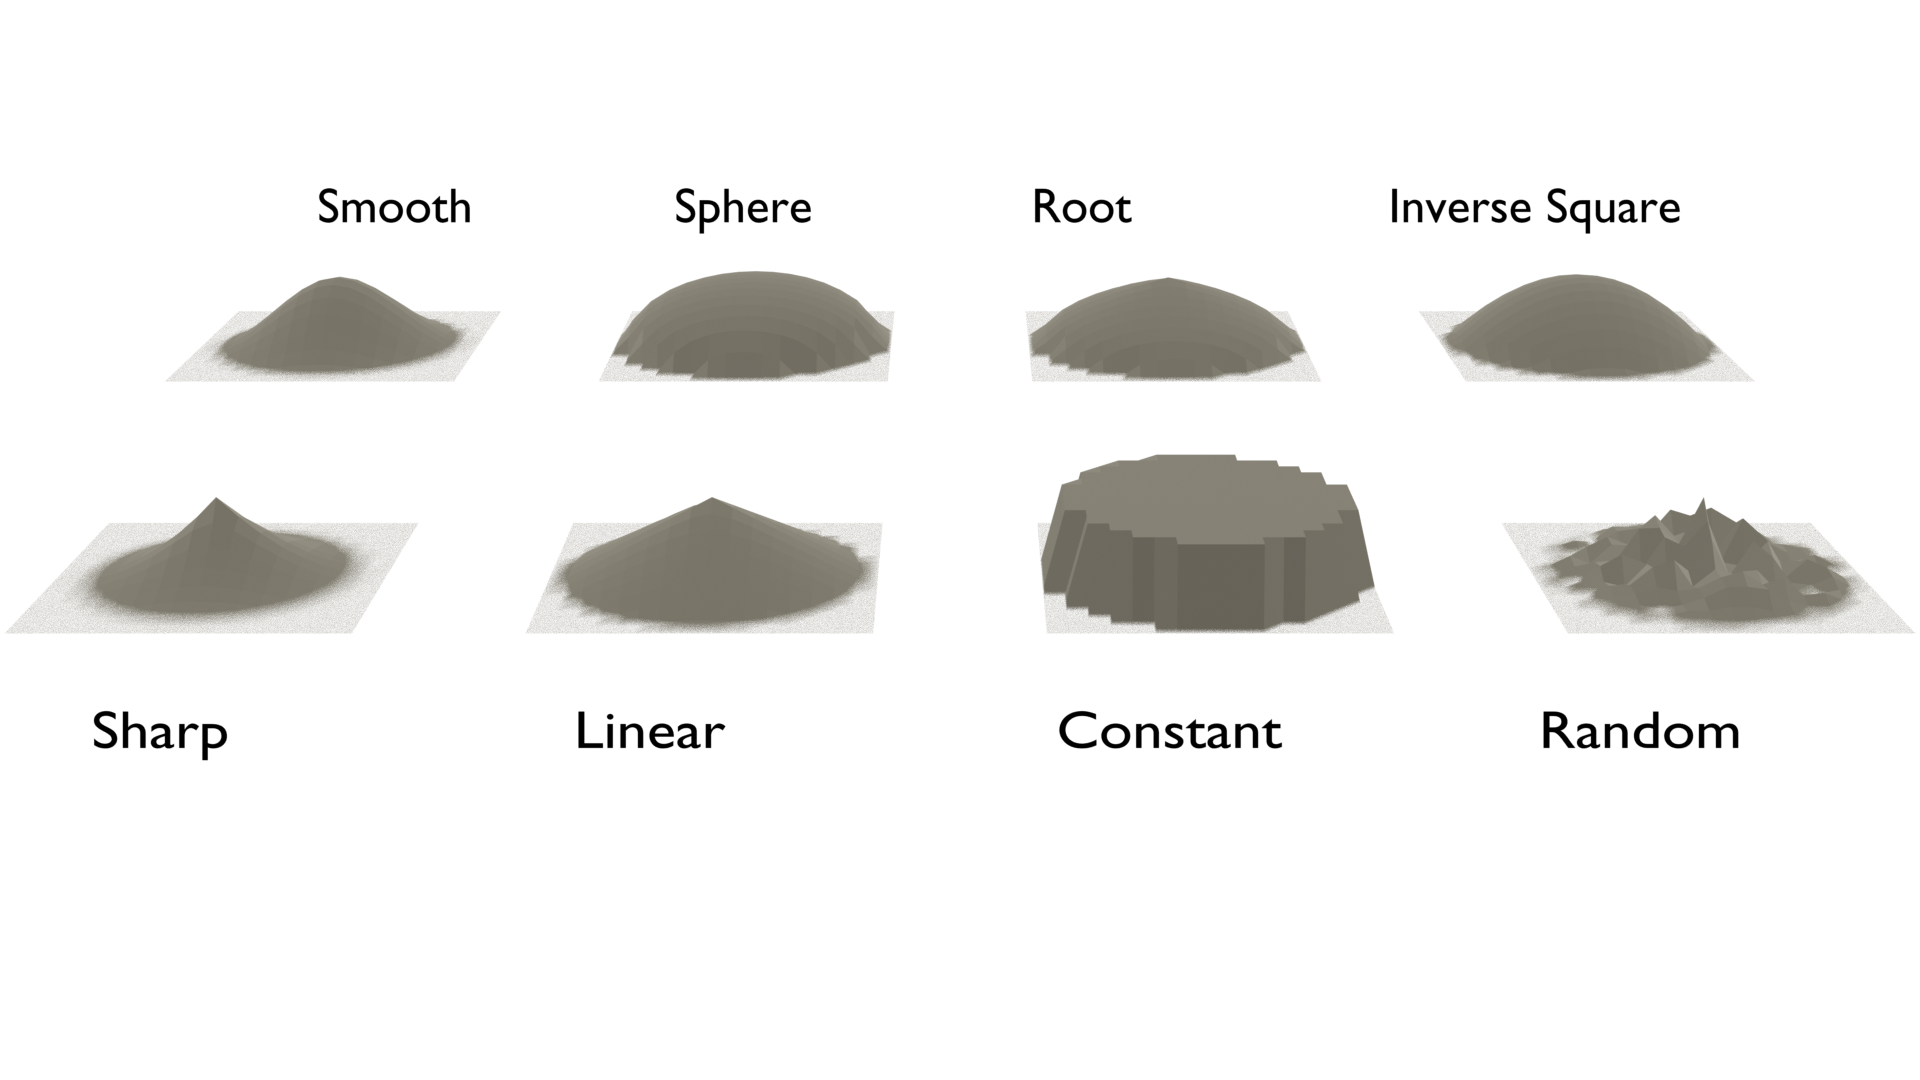
\includegraphics{Chapters/Images/Chapter_12/12_6_Proportional_Editing_Examples.png}

\caption{\label{fig-1_6}Die verschiedenen Formen zur proportionalen
Bearbeitung im Vergleich. Beispiele zeigen eine Fläche von 2x2 Metern,
bestehend aus 16x16 Faces. Diese Faces wurden mittig um 0.5 Meter
entlang der Z-Achse bewegt.}

\end{figure}%

\marginnote{Anwendungsbereiche für proportionale Bearbeitung}

Gerade natürliche Objekte (Früchte, Landschaften, Bäume, Blumen, usw.)
sind selten symmetrisch. Oftmals gibt es Dellen oder andere
Verformungen. Mittels der proportionalen Bearbeitung können solche
Verformungen leicht auf grössere Flächen angewendet werden, ohne dass
jeder Vertex einzeln bearbeitet werden muss.

Übung 8: Proportional Editing

\textbf{Übung 8.1}

Erstellen Sie eine UV-Sphere und versuchen Sie, damit eine Birne zu
modellieren. Nutzen Sie hierfür die proportionale Bearbeitung.

\section{Weitere Optionen}\label{weitere-optionen}

\marginnote{Symmetrische Bearbeitung}

Im Edit-Mode sind in der oberen rechten Ecke weitere Optionen verfügbar.
Zum einen sind die drei Achsen X, Y und Z als Schaltfläche anwählbar.
Durch das Anwählen eines dieser Icons wird das Objekt entsprechend der
ausgewählten Achse symmetrisch bearbeitet. Eine Veränderung des Objekts
auf der einen Seite der Achse wird dabei also gleichzeitig auch auf der
gegenüberliegenden Seite durchgeführt. Gerade bei symmetrischen Objekten
hat dies den Vorteil, dass der Fokus nur auf eine Seite gelegt werden
muss, ohne dass die Bearbeitungsschritte auf der anderen Seite nochmals
wiederholt werden müssen.

\marginnote{Symmetrische Bearbeitung zu Beginn aktivieren}

Bei der symmetrischen Bearbeitung muss allerdings darauf geachtet
werden, dass diese Option nicht immer funktioniert. Sobald die
Bearbeitung des Objektes begonnen hat, kann Blender teilweise diese
Symmetrie nicht mehr berücksichtigen. Wenn eine symmetrische Objektbe
arbeitung nötig ist, sollte diese also gleich zu Beginn aktiviert
werden.

\marginnote{Vertices automatisch verbinden}

Neben den Schaltflächen für die drei Achsen befindet sich zudem das Icon
für die Option «\emph{Auto Merge Vertices}». Durch das Aktivieren dieser
Option werden Vertices, welche während der weiteren Bearbeitung auf
derselben Position platziert werden, automatisch miteinander verbunden.
Dadurch ist es nicht mehr nötig, von Hand Vertices zu einem Vertex zu
verbinden.

\begin{figure}

\includegraphics{Chapters/Images/Chapter_12/12_7_Icon_Automerge.png}

\caption{\label{fig-1_7}Icon für Auto Merge Vertices.}

\end{figure}%

\chapter{Tutorial: Erstellen eines
Glases}\label{tutorial-erstellen-eines-glases}

\marginnote{Ziel dieses Tutorials}

Bislang wurden die grundlegenden Prinzipien der Objektbearbeitung
behandelt. Diese ermöglichen eine Vielzahl von
Bearbeitungsmöglichkeiten, sodass bereits sehr komplexe Objekte
modelliert werden können. Nachfolgend daher eine Erklärung, wie
beispielsweise die erläuterten Bearbeitungsmöglichkeiten verwendet
werden können, um ein Glas zu modellieren, wie etwa in Abbildung 1.

\marginnote{Würfel löschen}

Zunächst wird ein neues Blender-Projekt geöffnet. Da das Glas eine runde
Form hat, ist der Standardwürfel nicht geeignet, um das Glas
nachzubilden. Aus diesem Grund wird er mittels der Taste \kbd{X}
gelöscht.

\marginnote{Referenzbild einfügen}

Generell ist es empfehlenswert, bei der Erstellung von Objekten mit
Referenzbildern zu arbeiten. Aus diesem Grund wird eine Bildvorlage für
das Glas benötigt. Hierfür kann eine Bilddatei direkt aus einem Ordner
oder vom Desktop in den 3D-Viewport hineingezogen werden, sodass das
Bild anschliessend direkt in der Szene sichtbar wird. Das Bild wird
allerdings so eingefügt, dass es senkrecht zur Benutzeransicht sichtbar
ist. Das bedeutet, dass das Bild entsprechend der eigenen
Benutzeransicht positioniert und rotiert wird. Aus diesem Grund
empfiehlt es sich, vor dem Hineinziehen des Bildes mit der Taste \kbd{1}
in die Frontansicht zu wechseln. Dadurch wird das Bild lediglich entlang
der X-Achse um 90° rotiert eingefügt. Alternativ kann das Bild über das
«\emph{Add}»-Menü (\kbd{Shift} + \kbd{A}) unter «\emph{Image \textbar{}
Reference}» hinzugefügt werden. Zudem ist das Bild jeweils nur sichtbar,
wenn die Viewport-Overlays aktiviert sind.

\begin{figure}

\includegraphics{Chapters/Images/Chapter_13/13_1_Image_Example.png}

\caption{\label{fig-1_1}Bildvorlage zur Erstellung eines Glases.}

\end{figure}%

\marginnote{Bild platzieren}

Allenfalls sollte das Referenzbild noch im Raum platziert werden.
Idealerweise wird das Bild so platziert, dass sich der Mittelpunkt des
unteren Endes des Glases am Nullpunkt der Welt befindet. An dieser
Stelle sollte sich ebenfalls der 3D-Cursor befinden.

\marginnote{Primitive Mesh erstellen}

Als Nächstes wird das Objekt hinzugefügt, aus dem anschliessend das Glas
geformt werden soll. Dieses hat im Idealfall bereits eine ähnliche Form
wie das zu erstellende Objekt. In diesem Fall würde dies einem Zylinder
entsprechen. Über das «\emph{Add}»-Menü (\kbd{Shift} + \kbd{A}) wird
unter «\emph{Mesh \textbar{} Cylinder}» ein Zylinder an der Position des
3D-Cursors erstellt. Der Zylinder kann in seinen Default-Einstellungen
belassen werden.

\marginnote{Zylinder positionieren}

Mittels der Taste \kbd{Tab} wird in den Edit-Mode gewechselt, um die
Bearbeitung des Zylinders zu starten. Die Höhe des Zylinders erstreckt
sich nun von Z = -1m bis Z = 1m. Somit lieg ein Teil des Zylinders
unterhalb des Ursprungs des Objektes. Deshalb wird der Zylinder nun um
einen Meter entlang der Z-Achse nach oben verschoben. Mittels der Taste
\kbd{A} werden alle Elemente des Zylinders ausgewählt. Um eine
Verschiebung entlang der Z-Achse um einen Meter zu bewirken, wird die
Taste \kbd{G} zum Starten der Bewegung, die Taste \kbd{Z} zum Einrasten
entlang der Z-Achse, die Zahl \kbd{1} zur Angabe der Bewegung um einen
Meter und die Taste \kbd{Enter} zum Bestätigen gedrückt. Nun sollte der
Boden des Zylinders am Nullpunkt liegen, so wie in Abbildung 2.

\begin{figure}

\includegraphics{Chapters/Images/Chapter_13/13_2_Glass_Cylinder.png}

\caption{\label{fig-1_2}Zylinder, nachdem seine Vertices um einen Meter
entlang der Z-Achse nach oben verschoben wurden.}

\end{figure}%

\marginnote{Höhe des Zylinderdeckels anpassen}

Der Zylinder ist nun an der Position des Glases, allerdings weist er die
falschen Dimensionen auf. Durch eine Skalierung des Zylinders würde sich
auch der soeben angepasste Boden verschieben. Deshalb werden die
Vertices des Deckels manuell ausgewählt und verschoben. Hierfür wird bei
gedrückter \kbd{Alt}-Taste ein Edge entlang des Zylinderdeckels
ausgewählt. Dadurch werden alle Vertices entlang der Schlaufe dieses
Edges ausgewählt -- also in dem Fall alle Vertices auf dem Deckel des
Zylinders. Diese Vertices werden nun entlang der Z-Achse um den Wert
-1.2 verschoben, sodass sie die Höhe Z = 0.8 aufweisen.

\marginnote{Breite des Zylinders anpassen}

Als Nächstes wird der Mantel des Zylinders angepasst, sodass er der
maximalen Breite des Glases entspricht. Hierfür werden alle Vertices
ausgewählt und entlang der X- und Z-Achse kleiner skaliert. Mittels der
Taste \kbd{A} werden alle Vertices ausgewählt. Anschliessend wird
mittels der Taste \kbd{S} der Skalierungsvorgang gestartet, und mittels
der Tastenkombination \kbd{Shift} + \kbd{Z} die Z-Achse ignoriert. Durch
die Eingabe von \kbd{0} \kbd{.} \kbd{6} und der Bestätigung mittels
\kbd{Enter} wird anschliessend das Objekt entlang der X- und Y-Achse um
den Faktor 0.6 skaliert.

\marginnote{Zylindermantel in Edges unterteilen}

In den nächsten Bearbeitungsschritten muss der Mantel des Zylinders
entsprechend der Form angepasst werden. Hierfür werden weitere Vertices
Innerhalb des Zylindermantels benötigt. Um diese hinzuzufügen, werden
mit einem Loop Cut zehn Edges entlang des Zylindermantels eingefügt.
Hier für wird mit der Tastenkombination \kbd{Ctrl} + \kbd{R} zunächst
der Loop-Cut-Modus gestartet. Anschliessend wird der Mauszeiger über die
Edges, welche vertikal dem Zylindermantel entlang verlaufen, bewegt.
Dadurch sollte Blender nun einen Schnitt entlang des Zylindermantels in
der Mitte der Höhe vor schlagen. Um statt eines Schnittes gleich zehn
Schnitte zu erhalten, wird die Zahl \kbd{1} \kbd{0} eingegeben und der
Schnitt anschliessen mittels der linken Maustaste oder \kbd{Enter}
bestätigt. Danach muss nochmals mittels der linken Maustaste oder
\kbd{Enter} bestätigt werden, dass der Loop Cut mittig der Flächen
verlaufen soll. Wenn die Maus bereits bewegt wurde, erfolgt der Schnitt
nicht mehr mittig. In diesem Fall sollte die Platzierung mittels
\kbd{esc} der Taste beendet werden.

\marginnote{Anpassen der Breite von Hand}

Die neu erstellten Edges werden nun horizontal der Breite des Glases auf
der jeweiligen Höhe angepasst. Dies kann zum einen manuell von Hand für
jede Reihe an Edges erfolgen. Hierfür wird mittels \kbd{Alt} + der
linken Maustaste auf ein horizontales Edge die gesamte Reihe von Edges
ausgewählt. Mittels der Skalierung (\kbd{S}) entlang der X- und Y-Achse
(\kbd{Shift} + \kbd{Z}) kann der Radius für die entsprechende Höhe
eingestellt werden. Der Radius wird nacheinander für jede Edge-Reihe
angepasst.

\marginnote{Anpassen der Breite mittels Proportional Editing}

Alternativ kann auch auf das «\emph{Proportional Editing}»
zurückgegriffen werden, welches mittels der Taste \kbd{O} aktiviert
wird. Dadurch kann etwa die oberste Reihe von Edges mittels \kbd{Alt} +
der linken Maustaste ausgewählt werden. Anschliessend wird mittels der
Taste \kbd{S} die Skalierung gestartet. Für die proportionale
Bearbeitung wird nun ein Kreis dargestellt. Dieser kann mittels des
Mausrads verkleinert oder vergrössert werden. Sein Radius ist im oberen
Bildschirmrand angezeigt und sollte etwa 0.75 betragen. Anschliessend
kann die Skalierung entlang der X- und Y-Achse festgelegt (\kbd{Shift} +
\kbd{Z}) und um den Faktor 0.85 skaliert werden. Dieser Vorgang wird
anschliessend nochmals am unteren Rand des Zylinders wiederholt (mit
einem Radius von ca. 0.5 und einer Skalierung um den Faktor 0.5).
Anschliessend wird bei deaktivierter proportionaler Bearbeitung noch der
untere Rand erneut um den Faktor 0.9 entlang der X- und Y-Achse skaliert
und der obere Rand ebenfalls um den Faktor 0.975.

\marginnote{Zylinderdeckel löschen}

Der Zylinder sollte nun bereits die Form des Glases aufweisen. Durch
einen Wechsel in den Face-Select-Modus ist es möglich, direkt das Face,
welches den Deckel des Zylinders darstellt, auszuwählen und mittels
\kbd{X} zu löschen. Anschliessend ist das Glas so gut wie fertig -- ihm
fehlt lediglich noch eine Dicke.

\marginnote{3D-Cursor verschieben}

Um die Dicke des Glases zu erstellen, sollen alle Faces gegen den
Mittelpunkt des oberen Randes des Zylinders hinausgezogen werden.
Hierfür muss zunächst der 3D-Cursor mittig des oberen Randes platziert
werden. Dies geschieht, indem alle Edges entlang des oberen Randes
ausgewählt werden (hierfür muss wieder in den Edge- oder
Vertex-Select-Modus gewechselt werden). Anschliessend wird mittels der
Tastenkombination \kbd{Shift} + \kbd{S} das Snap-Menü geöffnet. Mit der
Auswahl «\emph{Cursor to Selected}» wird der 3D-Cursor mittig in der
Auswahl zu platzieren.

\begin{figure}

\includegraphics{Chapters/Images/Chapter_13/13_3_Proportional_Editing_Top.png}

\caption{\label{fig-1_3}Proportionale Anpassung der Breite des Zylinders
entsprechend der Bildvorlage.}

\end{figure}%

\marginnote{Fläche nach innen extrudieren}

Anschliessend wird der Bezugspunkt für Transformationen auf den
3D-Cursor gewechselt (unter der Schaltfläche «\emph{Transform Pivot
Point}» im Header). Nachdem alle Elemente des Zylinders mittels \kbd{A}
ausgewählt wurden, können nun alle Flächen mit der Taste \kbd{E}
extrudiert werden. Mittels der Taste \kbd{S} wird skalierend extrudiert
und mit den Tasten \kbd{0} \kbd{.} \kbd{9} \kbd{5} der Faktor 0.95
festgelegt. Dies kann schliessend mittels der linken Maustaste oder
\kbd{Enter} bestätigt werden. Mit diesem Schritt ist das Glas bereits
fertiggestellt. Es sieht noch etwas eckig und kantig aus, aber in den
nächsten Kapiteln wird behandelt, wie das Glas noch glatter erscheint.

\begin{figure}

\includegraphics{Chapters/Images/Chapter_13/13_4_Extrusion_Thickness.png}

\caption{\label{fig-1_4}Alle Faces des Glases werden zum 3D-Cursor hin
extrudiert, damit das Glas eine Dicke erhält.}

\end{figure}%

\section{Alternative Methode zur Erstellung eines
Glases}\label{alternative-methode-zur-erstellung-eines-glases}

\marginnote{Backup-Objekt erstellen}

Es gibt noch eine andere Methode zur Erstellung des Glases. Zur
Veranschaulichung dieser Methode kann im Object-Mode nach der Auswahl
des Glases mittels der Taste \kbd{D} ein Duplikat erstellt werden,
welches mit der Taste \kbd{H} versteckt werden kann. Dadurch bleibt
dieses Duplikat erhalten, sodass trotzdem die andere Methode ausprobiert
werden kann.

\marginnote{Querschnitt des Glases erstellen}

Nun wird das andere Glas im Edit-Mode bearbeitet. Das Ziel ist es
hierbei, dass ein Querschnitt des Glases entsteht. Diese Methode
erfordert den Vertex-Select-Mode. Mittels \kbd{A} + der linken Maustaste
wird ein Edge, welches vertikal dem Glas entlang verläuft, ausgewählt
und mittels der Tastenkombination \kbd{Ctrl} + \kbd{I} die Auswahl
umgekehrt. Nun wird diese Auswahl von Vertices mittels \kbd{X} gelöscht.
Dadurch sollten nun lediglich die Vertices übrigbleiben, die den Rand
eines Glases vertikal darstellen. Die äussersten Vertices werden
anschliessend extrudiert und auf ihrer jeweiligen Höhe am Nullpunkt der
Szene plaziert.

\marginnote{Kreisförmiges Herausziehen mittels des Spin-Tools}

Anhand eines solchen Querschnittes eines Glases kann nun mittels des
Spin-Tools kreisförmig die Form des Glases extrudiert werden. Hierfür
wird zunächst in der Toolbar das Spin-Tool aktiviert. Anschliessend
werden alle Vertices mit der Taste \kbd{A} ausgewählt. Durch das Ziehen
entlang einer der beiden «+»-Symbole des Spin-Gizmos kann anschliessend
das Glas kreisförmig aus dem Querschnitt herausgezogen werden. Im
Kontext-Menü zur letzten Aktion kann anschliessend der Radius noch auf
360° festgelegt werden und darunter «\emph{Auto Merge}» aktiviert
werden. Dadurch werden die beiden Enden des extrudierten Bereichs
zusammen verbunden. Zusätzlich kann unter «\emph{Steps}» noch die Anzahl
extrudierter Faces erhöht werden, um einen glatteren Kreis zu erhalten.

\begin{figure}

\includegraphics{Chapters/Images/Chapter_13/13_5_Cross_Section.png}

\caption{\label{fig-1_5}Querschnitt des Glases. Die in der Abbildung
ausgewählten Vertices müssen entlang der X- und Y-Achse noch zum
Ursprung des Objektes extrudiert werden.}

\end{figure}%

Übung 9: Eigenes Glas erstellen

\textbf{Übung 9.1}

Nehmen Sie ein rundes Glas aus Ihrem eigenen Haushalt, welches Sie
anschliessend in Blender nachbauen. Idealerweise nehmen Sie ein Glas
ohne weitere Oberflächenstrukturen. Machen Sie ein Foto von diesem Glas
von der Seite in einem möglichst rechten Winkel und verwenden Sie dieses
Foto anschliessend als Vorlage in einem Blender-Projekt. Bauen Sie
dieses Glas anschliessend als 3D-Objekt nach.

Speichern Sie das Glas zudem ab, um es in späteren Kapiteln verwenden zu
können.

\chapter{Objekterstellung mittels
Modifiern}\label{objekterstellung-mittels-modifiern}

\marginnote{Destruktive Objektbearbeitung}

Die bislang besprochenen Methoden der Objektbearbeitung stellen
destruktive Methoden dar. Bei destruktiven Methoden wird das Objekt so
abgeändert, dass es seine originale Form verliert. Ein Zylinder, der mit
destruktiven Methoden zu einem Glas modelliert wird, verliert also seine
Form als Zylinder.

\marginnote{Destruktive Bearbeitung ist schwer zurückzuverfolgen}

Durch die destruktive Objektbearbeitung ist es schwierig, wieder an
einen früheren Punkt der Bearbeitung zurückzukehren. Mittels der
Tastenkombination \kbd{Ctrl} + \kbd{Z} können zwar Schritte wieder
rückgängig gemacht werden, allerdings ist die Anzahl dieser Schritte
beschränkt. Zudem gehen diese Bearbeitungsschritte verloren, sobald
Blender geschlossen wird, sodass Bearbeitungsschritte von früheren
Blender-Sessions nicht rückgängig gemacht werden können.

\marginnote{Komplexität durch destruktives Vorgehen}

Gerade wenn komplexe Objekte bearbeitet werden, kann es vorkommen, dass
frühere Schritte sich später als Fehler herausstellen. Dann muss das
Objekt möglicherweise über komplexe Umwege wieder in den gewünschten
früheren Zustand zurückgebracht werden. Zudem können gewisse Schritte
zum einen Zeitpunkt dazu führen, dass andere Schritte zu einem späteren
Zeitpunkt komplexer werden.

\marginnote{Modifier zur nicht-destruktiven Bearbeitung von Objekten}

Wäre es von daher nicht praktisch, wenn Objekte mittels möglichst
simpler Parameter bearbeitet werden könnten, welche sich auch
nachträglich jederzeit wieder bearbeiten liessen? Genau hierfür gibt es
die sogenannten Modifier. Die Modifier ermöglichen eine
nicht-destruktive Form der Objektbearbeitung. Sie können als Funktionen
verstanden werden, welche auf ein Objekt angewendet werden und deren
Einstellungen jederzeit nachjustiert werden können.

\section{Ein glas mittels Modifiern
erstellen}\label{ein-glas-mittels-modifiern-erstellen}

\subsection{Vorbereitung}\label{vorbereitung}

\marginnote{Bisheriges Glas stellt eine komplexe Struktur dar}

Im vorherigen Kapitel wurde bereits behandelt, wie ein Glas mittels
destruktiver Methoden erstellt werden kann. Die Form des
fertiggestellten Glases kann noch verändert werden, allerdings ist es
komplex, die Vertices so zu bearbeiten, dass die Struktur erhalten
bleibt. Deshalb wird nun ein neues Glas mittels Modifiern erstellt.

\marginnote{Objekt auf einen einzelnen Vertex reduzieren}

Um ein neues Glas zu erstellen, wird in diesem Fall ein beliebiges
primitives Mesh erstellt. Danach werden im Edit-Mode (Wechsel mittels
\kbd{Tab}) alle Vertices ausgewählt (\kbd{A}). Anschliessend werden
diese Vertices alle zu einem einzigen Vertex zusammengefasst, indem
mittels der Taste \kbd{M} der Merge-Befehl «\emph{At Center}» aufgerufen
wird. Nun sollte nur noch ein einziger Vertex vorhanden sein. Dieser
sollte am Ursprung des Objektes platziert werden. Hierfür kann in der
Sidebar (Aufrufen mittels \kbd{N}) der Vertex im lokalen
Koordinatensystem am Nullpunkt platziert werden. Dieser Vertex stellt
nun den Mittelpunkt des Glasbodens dar.

\marginnote{Neue Vertices extrudieren}

Als Nächstes wird die Form des Glases im Querschnitt erstellt. Am besten
wird das Objekt in der Vorderansicht betrachtet. Zunächst wird der
Radius des Glasbodens festgelegt. Hierfür wird ein Edge entlang der
X-Achse beispielsweise um 0.1 Meter extrudiert ( \kbd{E}, \kbd{X},
\kbd{0} \kbd{.} \kbd{1}, danach bestätigen mittels der Taste
\kbd{Enter}). Anschliessend wird von diesem Vertex ebenfalls ein Vertex
herausgezogen, welches entlang der Z-Achse (und bei Bedarf auch entlang
der Y-Achse) verschoben wird. Dadurch sollte nun ein Querschnitt eines
halben Glases erstellt worden sein, wie in Abbildung 1 dargestellt.

\begin{figure}

\includegraphics{Chapters/Images/Chapter_14/14_1_Cross_Section.png}

\caption{\label{fig-1_1}Der Querschnitt eines halben Glases.}

\end{figure}%

\marginnote{Vertices mit der Maus erstellen}

Eine alternative Möglichkeit, um Vertices zu extrudieren, besteht darin,
dass im Edit-Mode bei gedrückter \kbd{Ctrl}-Taste mit der rechten
Maustaste in den 3D-Viewport geklickt wird. An der Stelle des Klicks
wird anschliessend ein neuer Vertex erstellt. Wenn davor ein Vertex
ausgewählt wurde, wird der mit dem Klick erstelle Vertex über ein Edge
mit dem ausgewählten Vertex verbunden. So kann der Umriss des Glases
auch mittels der Maus erstellt werden.

\marginnote{Weitere Schritte zur Erstellung des Glases}

Mithilfe dieser drei Vertices kann bereits ein Glas erstellt werden.
Hierfür wird Folgendes benötigt:

\begin{itemize}
\tightlist
\item
  Die drei Vertices müssen, wie mit dem Spin-Tool, im Kreis extrudiert
  werden.
\item
  Das Objekt benötigt eine Dicke.
\end{itemize}

\subsection{Hinzufügen von Modifiern}\label{hinzufuxfcgen-von-modifiern}

\marginnote{Modifier-Panel im Properties-Editor}

Modifier sind jeweils im Properties-Editor aufzufinden, welcher das
Areal in der rechten unteren Ecke von Blender darstellt. Auf der linken
Seite dieses Editors befindet sich ein Reiter mit verschiedenen
Symbolen. Die Modifier werden dort als Schraubenschlüssel symbolisiert.
Durch einen Klick auf den Schraubenschlüssel wird der Modifier-Reiter
geöffnet. Darin werden alle Modifier aufgelistet, die dem aktiven Objekt
oder dem gerade bearbeiteten Objekt zugewiesen sind.

\begin{figure}

\includegraphics{Chapters/Images/Chapter_14/14_2_Icon_Modifiers.png}

\caption{\label{fig-1_2}Modifier-Icon, welches im Reiter des
Properties-Editors aufzufinden ist.}

\end{figure}%

\marginnote{Modifier hinzufügen}

Der Reiter für die Modifier ist noch leer, da dem Objekt noch kein
Modifier hinzugefügt wurde. In der Dropdown-Liste «\emph{Add Modifie}r»
können Modifier hinzugefügt werden. Diese Modifier werden auf das aktive
Element oder das Objekt, welches gerade im Edit-Mode bearbeitet wird,
angewendet.

\marginnote{Screw-Modifier, um im Kreis zu extrudieren}

Als Erstes wird ein Modifier benötigt, der das Spin-Tool auf das Glas
anwendet. Dieser kann mittels des Modifiers «\emph{Screw}» erstellt
werden. Dieser Modifier extrudiert Objekte kreisförmig um den Ursprung
herum, analog zum Spin-Tool. Per Default wird das Objekt bei der
Anwendung des Modifiers um 360° im Kreis gedreht. Dadurch sollte aus dem
Querschnitt ein rundes Glas erstellt werden.

\marginnote{Veränderbarkeit von Modifiern}

Bei der destruktiven Methode mit dem Spin-Tool war es unerlässlich, dass
direkt bei der Durchführung der Transformation bestimmt wird, um wie
viele Grad die Operation durchgeführt werden soll, wie viele Faces
gebildet werden sollen und ob die Elemente automatisch verbunden werden
sollen. Bei der Bearbeitung mittels des Screw-Modifiers können diese
Einstellungen jederzeit in den Einstellungen des Modifiers verändert
werden. Für das aktuelle Glas-Objekt ist es sinnvoll, hier die
Einstellung «\emph{Merge}» zu aktivieren, sodass die Vertices am Start
und am Ende der Umdrehung zu je einem Vertex verbunden werden.

\begin{figure}

\includegraphics{Chapters/Images/Chapter_14/14_3_Glass_Screw_Solidify_Modifiers.png}

\caption{\label{fig-1_3}Glas, erstellt mittels eines Screw- und eines
Solidify-Modifiers.}

\end{figure}%

\marginnote{Solidify-Modifier, um Dicke zu erstellen}

Das Glas benötigt noch eine Dicke. Auch diese kann mittels eines
Modifiers hinzugefügt werden. Hierfür wird mittels des Dropdown-Menüs
«\emph{Add Modifier}» ein «\emph{Solidify}»-Modifier hinzugefügt. Dieser
extrudiert alle Faces entlang ihrer Normalen und verbindet sie
gemeinsam, sodass das Objekt eine Dicke erhält. Somit hat das Glas nun
bereits seine eigentliche Form erhalten.

\subsection{Der
Subdivision-Surface-Modifier}\label{der-subdivision-surface-modifier}

\marginnote{Subdivision Surface zum Glätten}

Das Glas ist allerdings sehr eckig. An dieser Stelle kommt der wohl
wichtigste Modifier zur Anwendung: der Subdivision-Surface-Modifier. Der
Subdivision-Surface-Modifier unterteilt alle Faces im Modell durch zwei
Edges in jeweils vier kleinere Faces -- so wie auch der Befehl
«\emph{Subdivide}». Zusätzlich passt der Modifier die neu gebildeten
Edges so an, dass die Oberflächen abgerundet und geglättet werden.
Dadurch können klobige und eckige Modelle besonders schnell zu
abgerundeten und glatten Modellen umgewandelt werden.

\marginnote{Subdivisions hinzufügen}

Unter «\emph{Add Modifier}» kann der «\emph{Subdivision
Surface}»-Modifier ausgewählt werden. Beim Modifier kann anschliessend
unter «\emph{Levels Viewport}» eingegeben werden, wie viele Subdivisions
erzeugt werden sollen. Es können maximal sechs Subdivisions im Modifier
durchgeführt werden (wobei auch mehr Subdivisions möglich sind, indem
ein weiterer Subdivision-Surface-Modifier hinzugefügt wird). Je höher
die Anzahl Subdivisions, desto glatter wird die Fläche. Allerdings
erhöht sich dadurch auch die Anzahl Vertices zur Berechnung des
Objektes, was mehr Leistung vom Computer erfordert. Es ist deshalb
ratsam, es nicht mit diesem Modifier zu übertreiben.

\marginnote{Subdivisions beim Rendern}

Unterhalb der Zeile «\emph{Levels Viewport}» befindet sich die Zeile
«\emph{Render}». Dadurch lässt sich die Anzahl Subdivisions für den
finalen Render einstellen. Dies ermöglicht eine höhere Anzahl
Subdivisions für den finalen Render-Prozess, während die Bearbeitung mit
einer geringeren Anzahl erfolgt und weniger Leistung benötigt wird.

\marginnote{Catmull vs. Simple}

Zusätzlich verfügt der Subdivision-Surface-Modifier über die
Einstellungsoption «\emph{Catmull-Clark}» oder alternativ
«\emph{Simple}». Per Default ist die Option «\emph{Catmull-Clark}»
eingestellt, welche dafür sorgt, dass das Objekt geglättet wird. Die
Option «\emph{Simple}» unterteilt das Objekt lediglich in mehr Vertices,
ohne deren Position so anzupassen, dass das Objekt glatter erscheint.

\section{Funktionsweise von
Modifiern}\label{funktionsweise-von-modifiern}

\marginnote{Fehlende Dicke}

Nun sollten dem Glas drei Modifier in der folgenden Reihenfolge
zugeordnet sein: ein Screw-Modifier, welcher die drei Vertices
kreisförmig extrudiert, ein Solidify-Modifier, welcher den Faces eine
Dicke hinzufügt, und ein Subdivision-Surface-Modifier, welcher das
Objekt durch zusätzliche Vertices glättet. Das Objekt erscheint nun
glatt, aber nicht mehr besonders dick. Dies liegt daran, dass der
Solidify-Modifier dem Glas eine Dicke zuweist, der
Subdivision-Surface-Modifier allerdings die Vertices dieser Dicke so
stark glättet, dass die Dicke wieder verschwindet. Zudem fällt auch auf,
dass der runde Boden des Glases stark verformt wird und
unverhältnismässig kantig erscheint.

\marginnote{Verwendung von Tris bei Modifiern}

Die seltsame Form am Boden ist auf die Form der Faces zurückzuführen,
welche durch die Modifier entstehen. Durch die kreisförmige Extrusion
der Vertices im Screw-Modifier entstehen am Boden eine Reihe Tris, die
sich kreisförmig um den Mittelpunkt bilden. Die meisten Modifier können
mit Tris umgehen, allerdings nicht alle gleich gut. In diesem Fall liegt
die Ursache beim Subdivision-Surface-Modifier, welcher die kreisförmigen
Vertices unterschiedlich stark zum Mittelpunkt hin glättet.

\begin{figure}

\includegraphics{Chapters/Images/Chapter_14/14_4_Tris_Bottom.png}

\caption{\label{fig-1_4}Verzerrung von Tris am Glasboden durch den
Subdivision-Surface-Modifier.}

\end{figure}%

\marginnote{Bevel-Modifier}

Sowohl das Problem der geringeren Dicke als auch das Problem der
unterschiedlich stark geglätteten Vertices am Glasboden kann mittels
eines zusätzlichen Modifiers behoben werden. Das Ziel hierfür ist, dass
alle Edges mit grösseren Winkeln abgerundet werden. Dies kann mittels
des Bevel-Modifiers erzielt werden. Dieser führt einen Bevel-Prozess in
einer nicht-destruktiven Methode durch. Unter «\emph{Add Modifier}» kann
«\emph{Bevel}» ausgewählt werden, um diesen Modifier hinzuzufügen.

\marginnote{Reihenfolge von Modifiern ändern}

Das Hinzufügen des Bevel-Modifiers reduziert das Problem der Dicke des
Glases, allerdings bleiben die Verformungen am Boden des Glases
bestehen. Dies liegt daran, dass der Bevel-Modifier noch vor dem
Subdivision-Surface-Modifier angewendet werden sollte, respektive der
Subdivision-Surface-Modifier nach dem Bevel-Modifier. In der rechten
oberen Ecke des Subdivision-Surface-Modifiers befindet sich eine
Schaltfläche. Bei gedrückter linker Maustaste auf diese Schaltfläche
lassen sich die Modifier verschieben. Es muss nun entweder der
Bevel-Modifier über den Subdivision-Surface-Modifier gezogen werden oder
der Subdivision-Surface-Modifier unterhalb des Bevel-Modifiers. Nun
sollten beide Probleme gelöst sein. Mittels eines Wertes von 2 für die
Subdivisions im Viewport müsste das Glas glatt aussehen.

\marginnote{Schaltflächen im Header des Modifiers}

Nebst der Schaltfläche zum Verschieben beinhaltet der Header eines
Modifiers noch weitere Punkte:

\begin{itemize}
\tightlist
\item
  Innerhalb eines Textfeldes wird der Name des Modifiers angezeigt.
  Dieser kann auch abgeändert werden, damit etwa die Funktion des
  Modifiers klarer wird.
\item
  Daneben sind drei weitere Schaltflächen anzutreffen, die wahlweise
  aktiviert oder deaktiviert werden können:

  \begin{itemize}
  \tightlist
  \item
    \textbf{On Cage}: Wenn diese Schaltfläche aktiviert ist, wird im
    Edit-Mode angezeigt, wie sich die Bearbeitung von Vertices auswirkt.
    Dieses Feld ist allerdings nicht bei allen Modifiern verfügbar. Da
    es beim Screw-Modifier nicht verfügbar ist, wird es im Beispiel mit
    dem Glas auch bei den nachfolgenden Modifiern nicht angezeigt. Durch
    das Deaktivieren der Schaltfläche «\emph{Edit Mode}» (siehe nächsten
    Aufzählungspunkt) beim Screw-Modifier wird die Schaltfläche
    «\emph{On Cage}» bei den darauffolgenden Modifiern jedoch wieder
    sichtbar.
  \item
    \textbf{Edit Mode}: Wenn diese Schaltfläche aktiviert ist, wird
    während der Bearbeitung im Edit-Mode der Effekt des Modifiers auf
    das gesamte Objekt gezeigt. Ansonsten bleibt dieser Modifier im
    Edit-Mode unberücksichtigt.
  \item
    \textbf{Realtime}: Der Modifier wird im 3D-Viewport angezeigt.
  \item
    \textbf{Render}: Der Modifier wird beim Rendern berücksichtigt.
  \end{itemize}
\item
  Innerhalb des Dropdown-Menüs sind folgende Optionen anzutreffen:

  \begin{itemize}
  \tightlist
  \item
    \textbf{Apply}: Der Modifier wird auf das Objekt angewendet. Dadurch
    verschwindet der Modifier aus der Ansicht und kann auch nicht mehr
    weiterbearbeitet werden. Wird zudem ein Modifier angewendet, der
    nicht an der obersten Position der Modifier-Reihenfolge liegt,
    werden alle vorgängigen Modifier bei der Anwendung ignoriert.
  \item
    \textbf{Duplicate}: Der Modifier wird dupliziert und direkt unter
    dem originalen Modifier platziert.
  \item
    \textbf{Copy to Selected}: Wenn mehrere Objekte ausgewählt sind,
    kann der Modifier des aktiven Elements durch diesen Befehl auf die
    anderen Objekte übertragen werden.
  \item
    \textbf{Move to First}: Der Modifier wird in der Reihenfolge der
    Modifier an die erste Stelle verschoben.
  \item
    \textbf{Move to Last}: Der Modifier wird in der Reihenfolge der
    Modifier an die letzte Stelle verschoben.
  \end{itemize}
\item
  Mittels des Kreuzes wird ein Modifier gelöscht.
\end{itemize}

Merke\ldots{}

Modifier werden verwendet, um Objekte nicht-destruktiv bearbeiten zu
können.

Modifier werden auf Objekte angewendet.

Wenn mehrere Modifier auf ein Objekt angewendet werden, werden sie
nacheinander in der Modifier-Ansicht von oben nach unten angewendet.

\section{Weitere Glättung erzielen durch
Smooth-Shading}\label{weitere-gluxe4ttung-erzielen-durch-smooth-shading}

\marginnote{Shade Smooth und Shade Flat}

Blender bietet eine Möglichkeit, um Objekte noch über den
Subdivision-Surface-Modifier hinaus zu glätten. Hierfür muss das
entsprechende Objekt im Object-Mode ausgewählt werden. Anschliessend
kann unter «\emph{Object \textbar{} Shade Smooth}» eingestellt werden,
dass das Objekt geglättet dargestellt wird. Unter «\emph{Object
\textbar{} Shade Flat}» kann ein geglättet dargestelltes Objekt wieder
ohne eine Glättung dargestellt werden.

\marginnote{Häufige Fehler beim Smooth-Shading}

Bei dieser Art der Glättung wird nichts an der Struktur des Objektes
geändert, sondern dessen Darstellung geglättet. Diese Darstellung wirkt
allerdings bei sehr kantigen Objekten und daher auch beispielsweise bei
Objekten im Low-Poly-Stil befremdlich. In diesem Fall ist eher «Shade
Flat» zu empfehlen. Zudem ist für die Berechnung dieser geglätteten
Fläche wichtig, dass die Normalen in die richtige Richtung orientiert
sind. Nebst zu kantigen Flächen sind falsch orientierte Normalen eine
häufige Ursache, wenn ein Objekt unter «Shade Smooth» schlecht
dargestellt wird.

\section{Die Vielzahl von Modifiern}\label{die-vielzahl-von-modifiern}

\marginnote{Vielfalt der Modifier}

Blender verfügt über eine sehr hohe Anzahl verschiedener Modifier,
welche auch stetig zunimmt. Einige dieser Modifier werden sehr selten
und für sehr spezifische Verfahren verwendet. Andere Modifier sind
hingegen praktisch unerlässlich für die Arbeit mit 3D-Objekten.

\marginnote{Arten von Modifiern}

Die verschiedenen Modifier sind in vier verschiedene Arten unterteilt:

\begin{itemize}
\tightlist
\item
  \textbf{Modify}: Diese Modifier fokussieren sich auf die Datenstruktur
  innerhalb der Meshes.
\item
  \textbf{Generate}: Diese Modifier ermöglichen eine nicht-destruktive
  Bearbeitung von Objekten.
\item
  \textbf{Deform}: Diese Modifier ermöglichen eine Veränderung der Form
  von Objekten.
\item
  \textbf{Physics}: Diese Modifier werden verwendet, um Objekten in
  Simulationen in Blender eine Rolle zuzuweisen.
\end{itemize}

\subsection{Generate-Modifier}\label{generate-modifier}

Für die Objekterstellung werden vor allem die Generate-Modifier
verwendet. Auf ihnen liegt deshalb auch der Fokus in diesem Kurs.

\subsubsection{Array}\label{array}

\marginnote{Objekte wiederholen mittels Array-Modifier}

Der Array-Modifier erstellt beliebig viele Duplikate eines Objektes.
Diese Duplikate werden in einer Reihe aufgestellt. Dadurch können sich
wiederholende Muster mittels dieses Modifiers erstellt werden. Hierfür
lässt sich die Anzahl Wiederholungen des Objektes unter «\emph{Count}»
einstellen. Anschliessend kann entlang der drei Achsen eingestellt
werden, in welchem Abstand die Wiederholungen jeweils zueinander stehen
sollen. Dieser Abstand kann relativ zur Grösse des Objektes eingestellt
werden, indem «\emph{Relative Offset}» aktiviert wird. In diesem Fall
wird der Abstand um einen Faktor relativ zur Objektgrösse definiert. Ein
Wert von 1 würde bedeuten, dass das Objekt direkt an der Stelle
wiederholt wird, an der das Original seine äusserste Grenze hat. Wenn
hingegen «\emph{Constant Offset}» aktiviert wird, werden die
Wiederholungen ausgehend vom Ursprung des Objektes um den angegebenen
Wert verschoben wiederholt. Beide Abstandsoptionen lassen sich zudem
miteinander kombinieren. Mittels der Einstellung «\emph{Merge}» lassen
sich zudem die wiederholten Objekte an den Vertices zwischen den
Wiederholungen verbinden -- vorausgesetzt diese befinden sich an
derselben Position.

\begin{figure}

\includegraphics{Chapters/Images/Chapter_14/14_5_Icon_Array_Modifier.png}

\caption{\label{fig-1_5}Icon für den Array-Modifier.}

\end{figure}%

\begin{figure}

\includegraphics{Chapters/Images/Chapter_14/14_6_Example_Array_Modifier.png}

\caption{\label{fig-1_6}Ein Objekt sowie eine Anwendung mittels eines
Array-Modifiers.}

\end{figure}%

\subsubsection{Bevel}\label{bevel-1}

\marginnote{Kanten abrunden mittels Bevel-Modifier}

Der Bevel-Modifier rundet die Kanten eines Objektes ab. Dabei kann
eingestellt werden, wie stark die Abrundung erfolgen soll und wie viele
Segmente für die Abrundung gebildet werden sollen. Zusätzlich kann eine
Abrundung auch auf Edges mit bestimmten Merkmalen fixiert werden
(beispielsweise nur Edges mit bestimmten Winkeln oder einer bestimmten
Datenstruktur). Zudem können auch Vertices abgerundet werden. Hierfür
muss im oberen Bereich des Modifiers «\emph{Vertices}» statt
«\emph{Edges}» ausgewählt werden.

\begin{figure}

\includegraphics{Chapters/Images/Chapter_14/14_7_Icon_Bevel_Modifier.png}

\caption{\label{fig-1_7}Icon für den Bevel-Modifier.}

\end{figure}%

\subsubsection{Boolean}\label{boolean}

\marginnote{Schnittmenge zwischen Objekten verwenden mittels Boolean-Modifier}

Der Boolean-Modifier wird verwendet, um die Teilmengen von zwei Objekten
zu bearbeiten. Hierfür wird im Modifier ein zweites Objekt ausgewählt.
Wahlweise kann anschliessend die gemeinsame Schnittmenge der beiden
Objekte ausgewählt («\emph{Intersect}»), verbunden («\emph{Union}») oder
entfernt werden («\emph{Difference}»). Zu beachten ist jedoch, dass beim
Verbinden (Union) beide Objekte lediglich zu einem Objekt miteinander
verbunden werden. Die Vertice-Strukturen der originalen Objekte bleiben
erhalten und werden nicht miteinander kombiniert. Bei den beiden anderen
Optionen werden die Vertices der beiden Objekte verbunden.

\begin{figure}

\includegraphics{Chapters/Images/Chapter_14/14_8_Icon_Boolean_Modifier.png}

\caption{\label{fig-1_8}Icon für den Boolean-Modifier.}

\end{figure}%

\begin{figure}

\includegraphics{Chapters/Images/Chapter_14/14_9_Example_Boolean_Modifier.png}

\caption{\label{fig-1_9}Der Boolean-Modifier eines Würfels in
Kombination mit einem Zylinder. Die drei verschiedenen
Boolean-Einstellungen führen zu unterschiedlichen Ergebnissen.}

\end{figure}%

\subsubsection{Build}\label{build}

\marginnote{Objekt-Aufbau animieren mittels Build-Modifier}

Der Build-Modifier ermöglicht es, dass ein Objekt im Rahmen einer
Animation sukzessive aufgebaut wird. Dabei lassen sich der Zeitpunkt des
Startes («\emph{Start Frame}») und die Dauer der Animation festlegen
(«\emph{Length}»).

\begin{figure}

\includegraphics{Chapters/Images/Chapter_14/14_10_Icon_Build_Modifier.png}

\caption{\label{fig-1_10}Icon für den Build-Modifier.}

\end{figure}%

\subsubsection{Decimate}\label{decimate}

\marginnote{Vertice in einem Objekt reduzieren mittels Decimat-Modifier}

Der Decimate-Modifier reduziert die Anzahl Vertices in einem Objekt.
Dabei wird das Objekt entweder um einen Faktor runtergebrochen
(«\emph{Collapse}»), «\emph{un-subdivided}» oder abgeflacht
(«\emph{Planar}»). Der Un-Subdivide-Modus stellt das Gegenteil des
Subdivision-Surface-Modifiers dar. In diesem Modus muss allerdings
beachtet werden, dass die Anordnung der Edges zwischen den Faces bei
jedem ungeraden Schritt der Un-Subdivision verändert wird, während sie
bei geraden Anzahlen Un-Subdivisions erhalten bleibt, wie in Abbildung
12 dargestellt.

\begin{figure}

\includegraphics{Chapters/Images/Chapter_14/14_11_Icon_Decimate_Modifier.png}

\caption{\label{fig-1_11}Icon für den Decimate-Modifier.}

\end{figure}%

\begin{figure}

\includegraphics{Chapters/Images/Chapter_14/14_12_Example_Unsubdivide.png}

\caption{\label{fig-1_12}Veränderung der Edge-Anordnung durch
Un-Subdivide.}

\end{figure}%

\subsubsection{Edge Split}\label{edge-split}

\marginnote{Edges zwischen Faces aufteilen mittels Edge-Split-Modifier}

Der Edge-Split-Modifier kann dazu verwendet werden, um Edges von zwei
aneinanderliegenden Faces aufzuteilen. Dadurch scheinen die Faces zwar
aneinanderzuliegen, allerdings handelt es sich dabei um zwei Faces, die
nicht miteinander verbunden sind. Dies hat den Vorteil, dass Kanten,
welche durch den Subdivision-Surface-Modifier abgerundet werden, nun als
einzelne Kanten betrachtet und nicht abgerundet werden. Hierfür muss der
Edge-Split-Modifier jedoch vor dem Subdivision-Surface-Modifier
platziert werden. Im Edge-Split-Modifier kann unter «\emph{Edge Angle}»
definiert werden, bis zu welchem Winkel die Edges jeweils separiert
werden sollen. Bei der Einstellung 30° werden alle Edges separiert,
deren Faces in einem grösseren Winkel als 30° zueinander stehen.

\begin{figure}

\includegraphics{Chapters/Images/Chapter_14/14_13_Icon_Edge_Split_Modifier.png}

\caption{\label{fig-1_13}Icon für den Edge-Split-Modifier.}

\end{figure}%

\subsubsection{Geometry Nodes}\label{geometry-nodes}

\marginnote{Objekte bearbeiten mittels Geometry-Nodes-Modifier}

Der Geometry-Nodes-Modifier ist ein relativ neuer Modifier in Blender.
Er wird benötigt, um ein Objekt mittels sogenannter Geometry Nodes zu
bearbeiten. Die entsprechende Einstellung des Geometry Nodes wird
jeweils im Geometry-Nodes-Editor vorgenommen.

\begin{figure}

\includegraphics{Chapters/Images/Chapter_14/14_14_Icon_Geometry_Nodes_Modifier.png}

\caption{\label{fig-1_14}Icon für den Geometry-Nodes-Modifier.}

\end{figure}%

\subsubsection{Mask}\label{mask}

\marginnote{Objekt-Teile maskieren mittels Mask-Modifier}

Mittels des Mask-Modifiers können Bestandteile eines Meshes versteckt
werden. Hierfür muss eine Gruppe aus Vertices definiert werden, welche
versteckt werdensoll, und diese Gruppe muss anschliessend im
Mask-Modifier angegeben werden. Wie Vertices zu Gruppen zusammengeführt
werden, wird im nächsten Kapitel behandelt.

\begin{figure}

\includegraphics{Chapters/Images/Chapter_14/14_15_Icon_Mask_Modifier.png}

\caption{\label{fig-1_15}Icon für den Mask-Modifier.}

\end{figure}%

\subsubsection{Mirror}\label{mirror}

\marginnote{Objekte spiegeln mittels Mirror-Modifier}

Der Mirror-Modifier spiegelt ein Objekt entlang ausgewählter Achsen vom
Ursprung des Objektes aus. Dadurch muss lediglich die Hälfte eines
symmetrischen Objektes erstellt oder bearbeitet werden, weil die zweite
Hälfte direkt mittels des Mirror-Modifiers erstellt wird. Mittels der
Funktion «\emph{Clipping}» kann zudem eingestellt werden, dass die
Punkte, welche direkt auf der Spiegelungsachse liegen, miteinander
verbunden werden und nicht mehr voneinander losgelöst werden können.

\begin{figure}

\includegraphics{Chapters/Images/Chapter_14/14_16_Icon_Mirror_Modifier.png}

\caption{\label{fig-1_16}Icon für den Mirror-Modifier.}

\end{figure}%

\subsubsection{Multiresolution}\label{multiresolution}

\marginnote{Mesh für Sculpting subdividen mittels Multiresolution-Modifier}

Der Multiresolution-Modifier führt bei einem Mesh eine Subdivision
durch, so wie auch der Subdivision-Surface-Modifier. Anders als beim
Subdivision-Surface-Modifier können diese Subdivisions jedoch beim
Sculpting von Objekten verwendet werden, ohne dass der Modifier
vorgängig auf das Objekt angewendet werden muss.

\begin{figure}

\includegraphics{Chapters/Images/Chapter_14/14_17_Icon_Multiresolution_Modifier.png}

\caption{\label{fig-1_17}Icon für den Multiresolution-Modifier.}

\end{figure}%

\subsubsection{Remesh}\label{remesh}

\marginnote{Mesh neu generieren mittels Remesh-Modifier}

Mithilfe des Remesh-Modifiers können die Vertices, Edges und Faces eines
Objektes neu generiert werden. Hierbei stehen verschiedene Möglichkeiten
zur Auswahl, wie Blender bei dieser Neugenerierung vorgehen soll:

\begin{itemize}
\tightlist
\item
  \textbf{\emph{«Blocks»}}: Die Form des Objektes wird blockartig
  erstellt.
\item
  \textbf{\emph{«Smooth»}}: Die Form des Objektes wird mit einer
  geglätteten Oberfläche er stellt.
\item
  \textbf{\emph{«Sharp»}}: Die Form des Objektes wird mit einer
  geglätteten Oberfläche erstellt, allerdings werden spitze Ecken und
  Kanten beibehalten.
\item
  \textbf{\emph{«Voxel»}}: Das Objekt wird basierend auf seinem Volumen
  neu erstellt.
\end{itemize}

\begin{figure}

\includegraphics{Chapters/Images/Chapter_14/14_18_Icon_Remesh_Modifier.png}

\caption{\label{fig-1_18}Icon für den Remesh-Modifier.}

\end{figure}%

\subsubsection{Screw}\label{screw}

\marginnote{Objekte kreisförmig extrudieren mittels Screw-Modifier}

Der Screw-Modifier wird verwendet, um Strukturen kreisförmig entlang
einer Achse um ihren Ursprung zu extrudieren. Zusätzlich kann ein
«\emph{Screw}»-Faktor definiert werden. Dieser verschiebt die Umdrehung
um den Screw-Faktor entlang der ausgewählten Achse, sodass eine
Schraubenform entsteht.

\begin{figure}

\includegraphics{Chapters/Images/Chapter_14/14_19_Icon_Screw_Modifier.png}

\caption{\label{fig-1_19}Icon für den Screw-Modifier.}

\end{figure}%

\subsubsection{Skin}\label{skin}

\marginnote{Vertices zu Mesh extrudieren mittels Skin-Modifier}

Der Skin-Modifier versieht den Vertices in einem Objekt eine zusätzliche
Haut in Form eines Würfels, der um den Vertex oder entlang der Edges
gebildet wird. So kann eine Form aus Vertices und Edges gebildet werden
und mittels des Skin-Modifiers mit einem Körper entlang der Edges
versehen werden. Dieser Modifier ist ähnlich zum Solidify-Modifier,
wobei der Skin-Modifier vor allem für Objekte ohne Faces verwendet wird.
Die Verwendung bei Objekten mit Faces in Kombination mit dem
Skin-Modifier kann sehr viel Rechenleistung erfordern.

\begin{figure}

\includegraphics{Chapters/Images/Chapter_14/14_20_Icon_Skin_modifier.png}

\caption{\label{fig-1_20}Icon für den Skin-Modifier.}

\end{figure}%

Durch das Hinzufügen des Skin-Modifiers ist es möglich, jeden Vertex
mittels einer Skalierung zu bearbeiten. Hierfür muss ein Vertex im
Edit-Mode ausgewählt werden. Mittels der Tastenkombination \kbd{Ctrl} +
\kbd{A} kann der Radius des Körpers bei diesem Vertex eingestellt
werden. Ohne das Hinzufügen des Skin-Modifiers steht diese Funktion
allerdings nicht zur Verfügung.

\begin{figure}

\includegraphics{Chapters/Images/Chapter_14/14_21_Example_Skin_modifier.png}

\caption{\label{fig-1_21}Ein Objekt aus Vertices und Edges sowie seine
Form mit dem Skin-Modifier.}

\end{figure}%

\subsubsection{Solidify}\label{solidify}

\marginnote{Faces extrudieren mittels Solidify-Modifier}

Der Solidify-Modifier wird verwendet, um Objekten eine Dicke
hinzuzufügen. Dabei werden alle Faces um den Wert der Dicke extrudiert.
Die Extrusion erfolgt entlang der Normalen eines Faces um einen
Offset-Wert. Wenn dieser Wert 1 oder -1 beträgt, werden die originalen
Vertices genau an derselben Stelle belassen und je nach Vorzeichen
verändert sich die Richtung der Extrusion. Bei einem negativen Wert
erfolgt die Extrusion entlang der Seite ohne Normalen, bei einem
positiven Wert entlang der Seite mit Normalen. Bei einem Wert von 0
werden die Flächen so gebildet, dass sich die originalen Faces genau in
der Mitte der neuen Faces befinden.

\begin{figure}

\includegraphics{Chapters/Images/Chapter_14/14_22_Icon_Solidify_Modifier.png}

\caption{\label{fig-1_22}Icon für den Solidify-Modifier.}

\end{figure}%

\begin{figure}

\includegraphics{Chapters/Images/Chapter_14/14_23_Example_Solidify_Modifier.png}

\caption{\label{fig-1_23}Ein Würfel ohne Deckel mit den Normalen nach
aussen gerichtet. Daneben Anwendungen des Solidify-Modifiers mit
unterschiedlichen Offset-Werten.}

\end{figure}%

\subsubsection{Subdivision Surface}\label{subdivision-surface}

\marginnote{Faces subdividen mittels Subdivision-Surface-Modifier}

Der Subdivision-Surface-Modifier wird verwendet, um die Struktur des
Objektes zu glätten, indem die Struktur des Objektes unterteilt wird.
Dieser Modifier wurde vorgängig ausführlich behandelt.

\begin{figure}

\includegraphics{Chapters/Images/Chapter_14/14_24_Icon_Subdivision_Surface_Modifier.png}

\caption{\label{fig-1_24}Icon für den Subdivision-Surface-Modifier.}

\end{figure}%

\subsubsection{Triangulate}\label{triangulate}

\marginnote{Quads zu Tris umwandeln mittels Triangulate-Modifier}

Der Triangulate-Modifier ermöglicht es, dass die Edges von Faces neu
berechnet werden, sodass die Faces lediglich aus Tris bestehen. Es
stehen dabei verschiedene Methoden zur Auswahl, welche individuell auf
Quads und N-Gons angewendet werden können. Durch eine Erhöhung der Zahl
unter «\emph{Minimum Vertices}» lässt sich einstellen, dass nur Faces
mit mindestens der entsprechenden Zahl von Vertices zu Tris umgewandelt
werden.

\begin{figure}

\includegraphics{Chapters/Images/Chapter_14/14_25_Icon_Triangulate_Modifier.png}

\caption{\label{fig-1_25}Icon für den Triangulate-Modifier.}

\end{figure}%

\subsubsection{Volume to Mesh}\label{volume-to-mesh}

\marginnote{Volumen zu Mesh umwandeln mittels Volume-to-Mesh-Modifier}

Mithilfe des Volume-to-Mesh-Modifiers können Volumen-Daten in ein Mesh
umgewandelt werden. Da dieser Kurs nicht auf Volumen-Objekte eingeht,
wird dieser Modifier nicht weiter behandelt.

\begin{figure}

\includegraphics{Chapters/Images/Chapter_14/14_26_Icon_Volume_to_Mesh-Modifier.png}

\caption{\label{fig-1_26}Icon für den Volume-to-Mesh-Modifier.}

\end{figure}%

\subsubsection{Weld}\label{weld}

\marginnote{Merge by Distance mittels Weld-Modifier}

Der Weld-Modifier stellt die Funktion «\emph{Merge by Distance}» als
Modifier dar. Dabei werden alle Vertices, die nahe beieinanderliegen, zu
einem Vertex zusammen gefasst. In den Einstellungen zum Weld-Modifier
kann unter «\emph{Distance}» festgelegt werden, bis zu welcher Distanz
die Vertices zusammengefasst werden sollen. Zudem kann unter
«\emph{Mode}» festgelegt werden, ob berücksichtigt werden soll, ob dies
nur auf miteinander verbundene Vertices («\emph{Connected}») oder alle
Vertices («\emph{All}») angewendet werden soll.

\begin{figure}

\includegraphics{Chapters/Images/Chapter_14/14_27_Icon_Weld_Modifier.png}

\caption{\label{fig-1_27}Icon für den Weld-Modifier.}

\end{figure}%

\subsubsection{Wireframe}\label{wireframe}

\marginnote{Gerüst um Mesh mittels Wireframe-Modifier}

Mithilfe des Wireframe-Modifiers werden die Flächen anhand eines
Gerüstes dargestellt. Die Edges der Faces werden hierfür aufgehoben und
mit vier Faces ersetzt, die entlang der Edges miteinander verbunden
werden. Die ursprünglichen Faces werden zusätzlich ebenfalls aufgehoben.
Der Wireframe-Modifier bezieht sich dabei lediglich auf die Faces:
Einzelne Edges, die nicht Teil eines Faces sind, werden dadurch entfernt
und nicht im Gerüst mit aufgenommen.

\begin{figure}

\includegraphics{Chapters/Images/Chapter_14/14_28_Icon_Wireframe_Modifier.png}

\caption{\label{fig-1_28}Icon für den Wireframe-Modifier.}

\end{figure}%

\marginnote{Gerüst anpassen}

Unter dem Reiter «\emph{Thickness}» in den Einstellungen zum
Wireframe-Modifier lässt sich einstellen, wie gross das Gerüst, welches
um die Edges herum gebildet wird, sein soll. Durch den
Wireframe-Modifier wird das originale Objekt per Default durch das
Gittergerüst ersetzt. Dies kann jedoch in den Einstellungen zum
Wireframe-Modifier unter «\emph{Replace Original}» deaktiviert werden,
sodass das originale Objekt nebst dem Gerüst bestehen bleibt.

\begin{figure}

\includegraphics{Chapters/Images/Chapter_14/14_29_Example_Triangulated Wireframe.png}

\caption{\label{fig-1_29}Würfel mit Triangulate- und
Wireframe-Modifier.}

\end{figure}%

Übung 10: Modifier

\textbf{Übung 10.1}

Erstellen Sie eine Wasserflasche mittels Modifiern. Verwenden Sie dabei
so wenige Vertices wie möglich.

\includegraphics{Chapters/Images/Chapter_14/Exercise_10_1.png}\hfill

\textbf{Übung 10.2}

Erstellen Sie einen Gartenzaun mittels Modifiern. Verwenden Sie dabei so
wenige Vertices wie möglich.

\includegraphics{Chapters/Images/Chapter_14/Exercise_10_2.png}\hfill

\section{Grenzen der Objektbearbeitung mittels
Modifiern}\label{grenzen-der-objektbearbeitung-mittels-modifiern}

\marginnote{Grenzen von Modifiern}

Wie beim Beispiel mit dem Glas zu erkennen ist, funktionieren Modifier
unter bestimmten Umständen nicht immer perfekt. Die Anwendung des
Subdivision-Surface-Modifiers auf einen Zylinder führt beispielsweise
dazu, dass nicht nur der Mantel des Zylinders abgerundet wird, sondern
auch die Kanten zum Boden beziehungsweise Deckel des Zylinders. Dies
führt dazu, dass der Zylinder seine Form verliert und eher einer Kugel
ähnelt. Der Boden und der Deckel des Zylinders stellen ein einzelnes
N-Gon dar. Durch die fehlenden Quads werden der Boden und der Deckel
somit in einer fehlerhaften Form abgerundet. In solchen Fällen macht die
Anwendung des Subdivision-Surface-Modifiers in dieser Form keinen Sinn.

\begin{figure}

\includegraphics{Chapters/Images/Chapter_14/14_30_Cylinder_Subdivison_Surface_Modifier.png}

\caption{\label{fig-1_30}Ein Zylinder mit einem
Subdivision-Surface-Modifier im Edit-Mode.}

\end{figure}%

\marginnote{Abrundung verhindern}

Es gibt einige destruktive Lösungsansätze, um die unerwünschten Effekte
des Subdivision-Surface-Modifiers zu reduzieren. So können
beispielsweise zusätzliche Loop Cuts (\kbd{Ctrl} + \kbd{R}) an den
Kanten hinzugefügt werden, welche zu stark abgerundet werden. Dies führt
dazu, dass Blender eine geringere Länge zur Verfügung hat, um Kanten
abzurunden.

\begin{figure}

\includegraphics{Chapters/Images/Chapter_14/14_31_Reduced_Smoothing_Loop_Cuts.png}

\caption{\label{fig-1_31}Reduzierte Glättung durch Loop Cuts.}

\end{figure}%

\marginnote{Abrundung von Tris/N-Gons verhindern}

Allerdings bleibt der Effekt einer ungenauen Abrundung entlang des
Deckels/Bodens bestehen. Um diesen Effekt zu reduzieren, kann das Face
des Deckels/Bodens ausgewählt und im Rahmen einer Extrusion kleiner
skaliert werden (Taste \kbd{E}, danach Taste \kbd{S}). Dadurch wird der
äusserste Rand des Deckels/Bodens mit Quads dargestellt, die gemeinsam
einen Kreis um ein paralleles N-Gon bilden (wie in Abbildung 32
dargestellt).

\begin{figure}

\includegraphics{Chapters/Images/Chapter_14/14_32_Quads_Smoothing_N_Gons.png}

\caption{\label{fig-1_32}Durch Quads am Rand wird das Glätten des N-Gons
verhindert.}

\end{figure}%

\marginnote{Parallelität, um Abrundung zu verhindern}

Die kreisförmig angeordneten Quads liegen in diesem Beispiel nun
parallel zu dem N-Gon in der Mitte. Dadurch erübrigt sich eine Glättung
des N-Gons entlang seiner Edges. Würde das N-Gon allerdings nicht
parallel verlaufen (z.B. wenn es weiter nach aussen gezogen würde, wie
in Abbildung 33), so würde das N-Gon wieder geglättet und eine
ungewollte Schraffierung entstünde erneut.

\marginnote{Bearbeitung von Meshes trotz Modifiern notwendig}

Dieses Beispiel zeigt, dass die nicht-destruktive Bearbeitung mittels
Modifiern teilweise auch Anpassungen im Mesh erfordern. Zudem ist es
teilweise nötig, dass Modifier auf ein Objekt angewendet werden, sodass
die Vertices, welche durch den Modifier entstehen, destruktiv
weiterbearbeitet werden können.

\begin{figure}

\includegraphics{Chapters/Images/Chapter_14/14_33_Smoothing_N_Gons.png}

\caption{\label{fig-1_33}Glättung des N-Gons entsteht wieder, wenn das
N-Gon nicht mehr parallel zu den umgebenden Quads liegt.}

\end{figure}%

\marginnote{Modifier auf Teilmengen des Meshes beschränken}

Es gibt allerdings auch noch Lösungsansätze, damit Modifier nicht auf
alle Elemente eines Meshes angewendet werden, oder sogar unterschiedlich
stark auf unterschiedliche Elemente eines Meshes angewendet werden.
Hierfür wird im nächsten Kapitel betrachtet, wie sich solche
Einstellungen für unterschiedliche Elemente innerhalb eines Meshes
einstellen lassen.

\chapter{Eigenschaften innerhalb eines Meshes
definieren}\label{eigenschaften-innerhalb-eines-meshes-definieren}

\section{Edge Crease}\label{edge-crease}

\marginnote{Subdivision-Surface-Modifier nicht auf alle Edges anwenden}

Im letzten Kapitel wurde gezeigt, wie der Effekt des
Subdivision-Surface-Modifiers reduziert werden kann. Hierfür wurde
erneut auf eine destruktive Bearbeitungsmethode zurückgegriffen. Es gibt
allerdings auch Möglichkeiten, um ohne eine destruktive Bearbeitung dem
Subdivision-Surface-Modifier mitzuteilen, dass er auf eine Anwendung an
bestimmten Stellen im Mesh verzichten soll. Hierfür wird der Edge Crease
verwendet.

\begin{figure}

\includegraphics{Chapters/Images/Chapter_15/15_1_Use_Edge_Creases_N_Gons.png}

\caption{\label{fig-1_1}Anwendung des Edge Creases auf ein N-Gon des
Zylinders.}

\end{figure}%

\marginnote{Edge Crease}

Der Edge Crease stellt ein Merkmal dar, welches einem Edge hinzugefügt
werden kann. Je höher der Edge Crease, desto geringer die Glättung durch
den Subdivision-Surface-Modifier. Der Edge Crease kann dabei Werte von 0
(normale Anwendung des Modifiers) bis 1 (keine Anwendung des Modifiers)
annehmen. Auch Abstufungen dazwischen sind möglich.

\marginnote{Edge Crease hinzufügen}

Um Edges einen Edge Crease hinzuzufügen, müssen sie zunächst ausgewählt
werden. Anschliessend kann mittels der Tastenkombination \kbd{Ctrl} +
\kbd{E} das «\emph{Edge}»-Menü beim Mauszeiger geöffnet werden und
«\emph{Edge Crease}» ausgewählt werden. Mittels der Bewegung des
Mauszeigers oder durch die Eingabe einer Zahl kann anschliessend der
Faktor für den Edge Crease festgelegt werden. Im Edit-Mode wird die
Stärke eines Creases für ein Edge jeweils mit einer violetten Markierung
angegeben. Eine besonders starke violette Markierung des Edges weist auf
einen Edge Crease von 1 hin, eine fehlende Markierung auf einen Edge
Crease von 0. Alternativ kann der Edge-Crease auch direkt über die
Tastenkombination \kbd{Shift} + \kbd{E} bei ausgewählten Edges verändert
werden.

\marginnote{Edge Creases über die Sidebar einstellen}

Nebst der Einstellung über das Edge-Menü kann der Edge Crease auch über
die Sidebar eingestellt werden. Unterhalb des Einstellungsfeldes für die
Position eines Vertex oder den Median der Auswahl befinden sich zwei
Felder für die Eingabe von «\emph{Edge Data}». Dort ist ein Feld für den
Crease des ausgewählten Edges zu finden. Wenn mehrere Edges ausgewählt
sind, wird der Mittelwert der Crease-Werte berechnet und an dieser
Stelle angezeigt. Durch das Ersetzen des Mittelwerts durch eine Zahl
wird der Crease proportional über die ausgewählten Elemente verändert,
sodass der Mittelwert diesem Wert entspricht. Durch die Eingabe von 0
werden generell alle Edge Creases bei der Auswahl entfernt und durch die
Eingabe von 1 werden generell alle Edge Creases bei der Auswahl
maximiert.

\marginnote{Edge Crease deaktivieren}

Per Default ist beim Subdivision-Surface-Modifier eingestellt, dass er
Edge Creases im Mesh berücksichtigt. Dies kann allerdings in den
Einstellungen zum Modifier unter dem Menü «\emph{Advanced}» unter
«\emph{Use Creases}» deaktiviert werden.

\section{Bevel Weight}\label{bevel-weight}

\marginnote{Edge Bevel Weight}

Nebst den Edge Creases, welche den Subdivision-Surface-Modifier steuern,
können die sogenannten Edge Bevel Weights verwendet werden, um den
Bevel-Modifier zu steuern. Bevel Weights können ebenfalls einen Wert von
0 bis 1 annehmen. Ein Wert von 0 steht allerdings für keine Anwendung
des Bevel-Modifiers und ein Wert von 1 für eine maximale Anwendung des
Bevel-Modifiers. Auch Abstufungen dazwischen sind möglich.

\begin{figure}

\includegraphics{Chapters/Images/Chapter_15/15_2_Stair_Bevel_Modifier.png}

\caption{\label{fig-1_2}Eine Treppe mit einem Bevel-Modifier.}

\end{figure}%

\marginnote{Edge Bevel Weight hinzufügen}

Um einem Edge einen Bevel Weight hinzuzufügen, muss das jeweilige Edge
ausgewählt werden. Anschliessend kann mit der Tastenkombination
\kbd{Ctrl} + \kbd{E} das «\emph{Edge}»-Menü beim Mauszeiger geöffnet
werden und «\emph{Edge Bevel Weight}» ausgewählt werden. Anschliessend
kann entweder mit einer Bewegung der Maus oder durch die Eingabe einer
Zahl der Edge Bevel Weight der Auswahl verändert werden. Im Edit-Mode
sind Edge Bevel Weights durch eine blaue farbliche Markierung entlang
der Edges ersichtlich. Je stärker die blaue Einfärbung, desto mehr
nähert sich der Edge Bevel Weight dem Faktor 1 an. Bei keiner farblichen
Markierung beträgt der Bevel Weight 0.

\begin{figure}

\includegraphics{Chapters/Images/Chapter_15/15_3_Stair_Edge_Bevel_Weights.png}

\caption{\label{fig-1_3}Eine Treppe mit Edge Bevel Weights auf und
zwischen den Stufen und einem Bevel-Modifier, der auf «Weight» limitiert
ist.}

\end{figure}%

\marginnote{Edge Bevel Weight im Viewport}

Wie auch der Edge Crease kann der Edge Bevel Weight in der Sidebar
eingestellt werden. Hierfür wird die Zeile «\emph{Bevel Weight}»
verwendet. Wie auch beim Crease lässt sich hier der Mittelwert der
Auswahl proportional anpassen, respektive der Wert 0 oder 1 für die
gesamte Auswahl fixieren.

\marginnote{Modifier auf Bevel Weights einstellen}

Der Bevel-Modifier berücksichtig die Edge Bevel Weights nicht in seinen
Default-Einstellungen. In ihm muss deshalb die Option «\emph{Limit
Method}» auf «\emph{Weigh}t» umgestellt werden. Dadurch wird der
Modifier nur auf Edges mit Bevel Weights angewendet.

\marginnote{Vertex Bevel Weight}

Bevel Weights können auch auf einzelne Vertices angewendet werden.
Hierfür können ausgewählten Vertices in der Sidebar unter «\emph{Vertex
Data}» ein Bevel Weight hinzugefügt werden. Vertex und Edge Bevel
Weights werden unabhängig voneinander zugeteilt und berechnet. Ein
Vertex, das Teil eines Edges mit einem Edge Bevel Weight von 1 ist, kann
einen anderen Vertex Bevel Weight aufweisen.

\marginnote{Modifier auf Vertex Bevel Weight einstellen}

Der Bevel-Modifier berücksichtigt die Vertex Bevel Weights lediglich,
wenn er auf «\emph{Vertices}» eingestellt wurde. Auch in diesem Fall
muss die «\emph{Limit Method}» auf «\emph{Weight}» eingestellt werden.
Wenn sowohl die Edge Bevel Weights als auch die Vertex Bevel Weights
berücksichtigt werden sollen, werden zwei Bevel-Modifier benötigt: ein
Modifier für die Vertex Bevel Weights und ein Modifier für die Edge
Bevel Weights.

\section{Vertex Groups}\label{vertex-groups}

\marginnote{Limitierung von Modifiern auf einzelne Vertices}

Durch den Edge Crease und den Bevel Weight stehen Möglichkeiten zur
Verfügung, um Elemente des Meshes graduell durch die Modifier bearbeiten
zu lassen. Für die meisten anderen Modifier steht eine solche graduelle
Anwendung nicht zur Verfügung. Es ist jedoch für sehr viele Modifier
möglich, dass die Anwendung lediglich auf einzelne Vertices angewendet
wird. Dadurch ist zwar keine graduelle Abstufung des Modifiers über das
Mesh möglich, allerdings eine Limitierung auf einzelne Vertices.

\marginnote{Vertex-Gruppen}

Im Edit-Mode können einzelne Vertices zu Gruppen zusammengefasst werden.
Solche Gruppen werden als Vertex Groups bezeichnet. Die Vertex-Gruppen
können über den Properties-Editor unter dem Reiter «\emph{Object Data
Properties}» anvisiert werden.

\begin{figure}

\includegraphics{Chapters/Images/Chapter_15/15_4_Icon_Vertex_Group.png}

\caption{\label{fig-1_4}Icon des «\emph{Object Data Properties}»-Reiters
im Properties-Editor.}

\end{figure}%

\marginnote{Vertex-Gruppe erstellen}

Durch einen Klick auf die «+»-Schaltfläche unter dem Reiter
«\emph{Vertex Groups}» in den Object Data Properties wird anschliessend
eine neue Vertex-Gruppe hinzugefügt, welche den Namen «Group» trägt.
Dieser Name kann beliebig angepasst werden und sollte -- gerade wenn
viele Vertex-Gruppen erstellt werden -- klar ausdrücken, welche Inhalte
diese Gruppe abdeckt.

\marginnote{Vertices zu Gruppen hinzufügen}

Wenn eine neue Vertex-Gruppe hinzugefügt wird, beinhaltet diese zunächst
keine Vertices. Diese müssen der neu erstellten Gruppe hinzugefügt
werden. Hierfür werden im Edit-Mode die entsprechenden Vertices
ausgewählt und anschliessend die Schaltfläche «\emph{Assign}» unterhalb
der Auflistung der Vertex-Gruppen betätigt. Dadurch werden der
Vertex-Gruppe die ausgewählten Vertices hinzugefügt. Analog können
mittels der Schaltfläche «\emph{Remove}» Vertices von bestehenden
Vertex-Gruppen entfernt werden.

\marginnote{Vertices mittels Vertex-Gruppen an- und abwählen}

Vertex-Gruppen sind auch nützlich, um einzelne Vertices schnell
auswählen zu können. Hierfür müssen diese einer Vertex-Gruppe zugewiesen
werden. Anschliessend kann diese Vertex-Gruppe markiert werden und
mittels der Schaltfläche «\emph{Select}» werden die Vertices, welche zu
dieser Auswahl gehören, im Objekt ausgewählt. Analog können mittels der
Schaltfläche «\emph{Deselect}» die Vertices einer Vertex-Gruppe von der
aktuellen Auswahl abgewählt werden.

\marginnote{Vertex-Gruppen sperren}

Es ist ausserdem möglich, bestehende Vertex-Gruppen zu sperren, sodass
keine weiteren Vertices der Vertex-Gruppe hinzugefügt oder von ihr
entfernt werden können. In der Auflistung der Vertex-Gruppen ist auf der
rechten Seite jeweils ein Schloss zu finden. Durch das Aktivieren dieses
Schlosses wird diese Vertex-Gruppe gesperrt. Dadurch wird verhindert,
dass aus Versehen neue Vertices der Gruppe hinzugefügt oder von ihr
entfernt werden.

\marginnote{Vertex-Gruppen zu Modifiern hinzufügen}

Bei vielen Modifiern lassen sich innerhalb der Einstellungen
Vertex-Gruppen in einer Zeile mit der Beschriftung «\emph{Vertex Group}»
auswählen. Wenn eine Vertex-Gruppe für ein Objekt definiert wurde, wird
diese anschliessend auswählbar für dieses Feld. Dadurch können die
entsprechenden Modifier auf diese Vertex-Gruppen beschränkt werden.
Beispielsweise kann der Bevel-Modifier statt mit Bevel Weights auch mit
Vertex-Gruppen auf einzelne Edges oder Vertices reduziert werden.

Übung 11: Objekterstellung mit Mesh-Daten

\textbf{Übung 11.1}

Verändern Sie den Standardwürfel mittels Modifiern und Mesh-Daten so,
dass das unten abgebildete Objekt dargestellt wird.

\hfill
\includegraphics{Chapters/Images/Chapter_15/Exercise_11_1.png}

\textbf{Übung 11.2}

Erstellen Sie mittels Modifiern das unten abgebildete Objekt.

\hfill
\includegraphics{Chapters/Images/Chapter_15/Exercise_11_2.png}

\chapter{Materialien, Texturen und
Shader}\label{materialien-texturen-und-shader}

\marginnote{Fokus auf Materialien}

Bislang lag der Fokus dieses Kurses auf der Erstellung von Objekten. Die
Objekte haben sich lediglich in ihrer Form unterschieden, aber nicht
hinsichtlich des Materials, aus dem sie bestehen. Im nächsten Schritt
wird die Bedeutung der Materialien behandelt, welche Mechanismen diesen
zugrunde liegen und wie diese auf Objekte angewendet werden.

\marginnote{Material}

\begin{itemize}
\tightlist
\item
  In den nächsten Kapiteln werden daher drei Begriffe von grosser
  Bedeutung sein: Materialien, Texturen und Shader. Beim Material
  handelt es sich dabei um ein Merkmal, welches einem Objekt oder einem
  Teil des Objektes zugewiesen wird. Das Material beschreibt sowohl, was
  auf der Oberfläche des Objektes (oder in dessen Volumen) abgebildet
  wird, als auch, wie dies dargestellt wird.
\end{itemize}

\marginnote{Parameter}

\begin{itemize}
\tightlist
\item
  Innerhalb des Materials wird eine Reihe verschiedener Parameter
  festgelegt, um eine Vielfalt an Materialien abdecken zu können. Diese
  Parameter können etwa die Farbe des Materials, aber auch Merkmale der
  Lichtreflexion beinhalten. Solche Parameter können einheitlich über
  das ganze Material angewendet werden (z.B. das ganze Material ist
  überall rot und reflektiert überall gleich stark), oder strukturell
  variieren (z.B. das Material stellt eine rote Mauer mit weissen Fugen
  dar -- dabei weisen die Fugen eine andere Farbe auf und haben
  allenfalls auch eine andere Reflexion).
\end{itemize}

\marginnote{Texturen}

\begin{itemize}
\tightlist
\item
  Um Parameter über Flächen hinweg variieren zu können, werden Texturen
  benötigt. Texturen sind Bilddokumente, welche dem Material zugwiesen
  werden und dadurch auch dem Objekt zugewiesen werden können. Eine
  Textur als solche wird jedoch nicht direkt auf ein Objekt angewendet,
  sondern als Material. Die wohl bekannteste Form der Texturen
  beschreibt, wie sich die Farbe des Materials über die Fläche des
  Objektes verändert. Allerdings können Texturen auch verwendet werden,
  um andere Parameter über die Fläche hinweg zu variieren.
\end{itemize}

\marginnote{Shader}

Shader stellen Verarbeitungseinheiten der Parameter/Texturen dar. Sie
bekommen Informationen aus den Parametern oder Texturen und verarbeiten
diese weiter. Ein Emission-Shader nimmt beispielsweise jeweils die
Parameter für die Farbe und strahlt diese um den Wert eines weiteren
Parameters aus. Andere Shader berücksichtigen zusätzlich das Licht aus
der Umgebung und verarbeiten die Parameter und Texturen in Abhängigkeit
dieser Lichtquellen oder unter Berücksichtigung weiterer Parameter.

\marginnote{Materialien, Texturen und Shader}

Ein Material beinhaltet somit sowohl Parameter oder Texturen, welche
Informationen beinhalten, als auch die Shader, welche die Informationen
verarbeiten. Blender ist mit einer Reihe von eigenen Shadern
ausgestattet, mit denen man arbeiten kann. Es ist allerdings auch
möglich, eigene Shader zu erstellen oder die Verarbeitung der
Informationen zu verändern.

\begin{figure}

\includegraphics{Chapters/Images/Chapter_16/16_1_Materials_Textures_Shader.png}

\caption{\label{fig-1_1}Zusammenhang zwischen Materialien, Texturen und
Shadern.}

\end{figure}%

\chapter{Materialien}\label{materialien}

\section{Bedeutung von Materialien}\label{bedeutung-von-materialien}

\marginnote{Wozu werden Materialien benötigt?}

In den bisherigen Übungen und Aufgaben wurden jeweils Objekte erstellt
und es war klar, was diese Objekte darstellen. Ein Haus stellte anhand
seiner geometrischen Figur ein Haus dar, ebenso verhielt es sich bei
einem Koffer oder auch bei einem Glas. Doch gerade beim Glas kann die
Wahrnehmung des Objektes erheblich durch dessen Material beeinflusst
werden.

\marginnote{Was stellt das Objekt dar?}

Zur Veranschaulichung: Das Bild in Abbildung 1 stellt dar, wie Objekte
bislang in diesem Kurs betrachtet wurden. Die Oberfläche war für alle
Objekte identisch, sodass zumindest erkennbar war, dass eine Oberfläche
vorhanden ist. Für eine aussenstehende Person muss nicht zwingen klar
sein, dass es sich bei diesem Objekt um ein Glas handelt. Es könnte sich
auch um einen Becher handeln, der aus Plastik besteht, oder allenfalls
um einen Pappbecher. Abbildung 2 zeigt mögliche Interpretationsbeispiele
für dieses Objekt auf. Alle diese Beispiele zeigen dasselbe Mesh mit
denselben Vertices, Edges und Faces. Sie unterscheiden sich allerdings
hinsichtlich der ihnen hinzugefügten Materialien.

\begin{figure}

\includegraphics{Chapters/Images/Chapter_17/17_1_Glass_without_Materials.png}

\caption{\label{fig-1_1}Ein Objekt im Solid-Shading-Modus.}

\end{figure}%

\marginnote{Objekt-Benennung durch Materialien}

Durch die Anwendung von Materialien kann also die Wahrnehmung der
Objekte verändert werden. Ein Glas erscheint als Glas, weil es eine
gewisse Transparenz aufweist. Andere Materialien verfügen über
unterschiedliche Farben und können so voneinander abgegrenzt werden.
Hierfür gibt es verschiedene Merkmale der Materialien, welche noch
ausführlich beschrieben werden.

\begin{figure}

\includegraphics{Chapters/Images/Chapter_17/17_2_Glass_or_Mug.png}

\caption{\label{fig-1_2}Ein Objekt mit unterschiedlichen Materialien.}

\end{figure}%

\section{Materialien betrachten}\label{materialien-betrachten}

\marginnote{Viewport-Shading-Modus wechseln}

Damit Materialien betrachtet werden können, ist ein Wechsel in der
Benutzeroberfläche in Blender nötig. Bislang wurden Objekte im
Solid-Viewport-Shading-Modus betrachtet. In diesem Modus werden die
Materialien von Objekten nicht für die Darstellung berücksichtigt. Um
die Materialien ebenfalls betrachten zu können, wird deshalb ein
Viewport-Shading-Modus benötigt, der die Materialien ebenfalls
darstellt. Hierfür kann der Material-Preview-Modus oder der
Render-Preview-Modus verwendet werden. Beide Einstellungen sind in der
rechten oberen Ecke des Viewport-Displays anwählbar. Durch das Drücken
der Taste \kbd{Z} erscheint zudem bei der Maus ein Kontext-Menü, welches
die verschiedenen Modi zur schnellen Auswahl anbietet.

\marginnote{Material-Preview-Modus verwenden}

Zum jetzigen Zeitpunkt des Kurses ist der Render-Preview-Modus noch
nicht zu empfehlen. Dieser Modus berücksichtigt die Lichtquellen und
Lichtreflexionen, welche in der Welt dargestellt werden. Dadurch ist es
teils schwer abzuschätzen, ob Probleme im Material auf dem Material oder
der umgebenden Beleuchtung beruhen. Deshalb wird an dieser Stelle der
Material-Preview-Modus verwendet. Dieser stellt die Materialien dar und
liefert vorgefertigte Beleuchtungsszenarien für die Welt.

\marginnote{Material-Preview-Modus}

Durch einen Klick auf die Schaltfläche für den Material-Preview-Modus
verändert sich die Darstellung der Oberfläche der Meshes. Blender
generiert die Materialien, welche dem Mesh zugewiesen sind, und
präsentiert diese basierend auf den Einstellungen der Welt -- in diesem
Fall basierend auf den Einstellungen der Vorschau-Welt.

\section{Materialien hinzufügen}\label{materialien-hinzufuxfcgen}

\marginnote{Default-Material}

Jedes Objekt wird im Material-Preview-Modus und im Render-Modus mit
einem Material dargestellt. In einer neuen Szene verfügt der
Standardwürfel bereits über ein vorgegebenes Material, welches
abgeändert werden kann. Ein neu in die Szene hinzugefügtes Objekt wird
ebenfalls mit einem Material dargestellt. Im Gegensatz zum
Standardwürfel ist dieses Objekt aber eigentlich noch nicht mit einem
Material ausgestattet.

\marginnote{Material-Reiter}

Um das Material eines Objektes aufzurufen, kann der Material-Reiter im
Properties-Editor aufgerufen werden. Unter diesem Reiter werden die
Materialien des aktiven Objektes aufgelistet. Wenn mehrere Objekte
ausgewählt sind, werden nur die Materialien des aktiven Objekts
dargestellt. Die Materialien sind unabhängig davon ersichtlich, ob
aktuell der Object- oder der Edit-Mode ausgewählt ist.

\begin{figure}

\includegraphics{Chapters/Images/Chapter_17/17_3_Material_Properties_Pannel.png}

\caption{\label{fig-1_3}Das Properties-Panel mit dem ausgewählten
Material-Reiter.}

\end{figure}%

\marginnote{Fehlendes Material}

Wenn ein Objekt noch über kein Material verfügt, ist der Material-Reiter
noch leer. Es gibt lediglich folgende Bereiche:

\begin{itemize}
\tightlist
\item
  \textbf{Leeres Feld}: Darin werden alle Slots für die Materialien
  eines Objekts aufgelistet.
\item
  «\textbf{+}»: Dadurch lässt sich ein neuer Slot für Materialien
  erstellen.
\item
  «\textbf{-}»: Dadurch lässt sich ein ausgewählter Slot für Materialien
  entfernen.
\item
  «\textbf{\emph{New}}»: Dadurch lässt sich ein neues Material
  erstellen.
\end{itemize}

\marginnote{Slots für Materialien}

Wenn nun die Schaltfläche «+» betätigt wird, erscheint ein neuer
Material-Slot für ein Material in dem Feld, welches vorher leer war.
Wichtig ist dabei, dass dies lediglich einen Platzhalter für ein
Material darstellt -- es wurde noch kein Material hinzugefügt. Durch das
erneute Klicken der Taste «+» erscheint ein weiterer Slot für
Materialien. Durch das Betätigen der Taste «-» wird dieser Slot wieder
entfernt.

\marginnote{Neues Material erstellen}

Durch das Drücken der Schaltfläche «\emph{New}» wird ein neues Material
erstellt. Dieses neue Material wird mit der Beschriftung
«\emph{Material}», und allenfalls gefolgt von einer Nummer hinter der
Bezeichnung, an der Stelle angezeigt, an der sich vorher die
Schaltfläche «\emph{New}» befunden hat. Zusätzlich wird das Material nun
in der Auflistung der Materialien im darüberliegenden Feld angezeigt.
Durch das Hinzufügen eines Materials wird automatisch ein Slot erstellt,
selbst wenn die Auflistung der Slots noch leer war. Wenn ein Slot
vorhanden ist, dieser aber noch leer ist, wird das Material diesem Slot
hinzugefügt.

\marginnote{Materialien ausdemselben Dokument wieder verwenden}

Statt ein neues Material zu erstellen, können auch Materialien, die
bereits in demselben Blender-Dokument erstellt wurden, dem Material-Slot
zugewiesen werden. Hierfür muss statt auf die Schaltfläche «\emph{New}»
auf das Dropdown-Menü links dieser Schaltfläche geklickt werden. Darin
werden alle Materialien aufgeführt, die bereits in diesem Dokument
vorhanden sind. Durch die Auswahl eines dieser Materialien wird dieses
Material anschliessend auch auf das Objekt angewendet. Dabei ist
allerdings zu beachten, dass dadurch keine Kopie des Materials erstellt
wird. Wird das Material etwa auch von einem anderen Objekt verwendet, so
führt eine Veränderung des Materials auch bei diesem Objekt zu einer
Veränderung.

\marginnote{Einstellungsoptionen der Materialien}

Durch die Auswahl oder die Erstellung eines Materials erscheint eine
Reihe von Einstellungsoptionen innerhalb des Material-Reiters. Diese
sind in folgende Bereiche gegliedert:

\begin{itemize}
\tightlist
\item
  «\textbf{\emph{Preview}}»: Darin wird eine Vorschau des Materials für
  verschiedene Objektarten angeboten.
\item
  «\textbf{\emph{Surface}}»: Darin werden die grundlegenden
  Einstellungen der Oberflächenbeschaffenheit des Materials vorgenommen.
\item
  «\textbf{\emph{Volume}}»: Darin können Eigenschaften für das Volumen
  des Materials definiert werden.
\item
  «\textbf{\emph{Settings}}»: Darin können weitere Einstellungen für die
  Darstellung des Materials vorgenommen werden.
\item
  «\textbf{\emph{Line Art}}»: Darin können Parameter für die Erstellung
  von Linien eingestellt werden, wenn die Erstellung von Linien
  aktiviert ist.
\item
  «\textbf{\emph{Viewport Display}}»: Darin können grundlegende
  Material-Eigenschaften für die Darstellung des Materials im
  Solid-Modus erstellt werden. Diese Eigenschaften dienen lediglich der
  Zurechtfindung im Solid-Modus und haben keinen Einfluss auf die
  Darstellung des Materials im finalen, gerenderten Produkt.
\item
  «\textbf{\emph{Custom Properties}}»: Darin können eigene Eigenschaften
  für ein Material definiert werden. Eine grosse Bedeutung kommt den
  Einstellungsoptionen im Reiter «\emph{Surface}» zu. Diese werden
  fortan benötigt, um die Materialien zu bearbeiten, während die anderen
  Optionen noch nicht berücksichtigt werden.
\end{itemize}

\marginnote{Use Nodes}

Im Reiter «\emph{Surface}» wird zuoberst die Schaltfläche «\emph{Use
Nodes}» blau eingefärbt dargestellt. Dies bedeutet, dass die Einstellung
der Oberfläche innerhalb des Shader-Editors bearbeitet werden kann. Die
meisten der Einstellungen im Material-Reiter können in diesem Editor
erfolgen. Zudem bietet dieser Editor eine Reihe Möglichkeiten, um die
Materialien noch genauer zu bearbeiten. Deshalb ist es empfehlenswert,
den Shader-Editor zu verwenden.

\chapter{Der Shader-Editor}\label{der-shader-editor}

\marginnote{Shader-Editor öffnen}

Um den Shader-Editor zu öffnen, sollte ein neues, zusätzliches
Editor-Fenster geöffnet werden. Dieses kann aus den Ecken des
3D-Viewport-Editors herausgezogen werden. In diesem neuen Fenster kann
anschliessend der 3D-Viewport-Editor zum Shader-Editor geändert werden.

\marginnote{Auswahl von Materialien im Shader-Editor}

Im Shader-Editor wird jeweils mittels einer grafischen
Programmiersprache durch die Verbindung von Nodes (Knotenpunkten)
definiert, wie die Materialien erstellt werden. In der Kopfleiste des
Editors wird zudem dasselbe Feld zum Auswählen respektive zum Hinzufügen
von Materialien angezeigt wie im Material-Reiter im Properties-Editor.
Die Auswahl eines anderen Materials im Shader-Editor führt dazu, dass
auch das Material im Properties-Editor sowie im Material-Slot
automatisch angepasst wird. Umgekehrt führt eine andere Auswahl eines
Materials im Properties-Editor dazu, dass im Shader-Editor automatisch
auch das entsprechende Material ausgewählt wird.

\marginnote{Darstellung eines Default-Materials im Shader-Editor}

Sofern ein Material ausgewählt ist, sollten sich innerhalb des
Shader-Editors zwei Blöcke befinden. Ein etwas grösserer Block, welcher
mit «\emph{Principled BSDF}» beschrieben ist, und ein kleinerer Block,
der als «\emph{Material Output}» beschriftet ist, wie in Abbildung 1
dargestellt. Beide Blöcke sind zwischen zwei grünen Punkten mittels
eines Fadens miteinander verbunden.

\begin{figure}

\includegraphics{Chapters/Images/Chapter_18/18_1_Default_Material.png}

\caption{\label{fig-1_1}Ein Principled-BSDF-Shader, der mit dem
Material-Output verbunden ist. Dies wird standardmässig bei einem neuen
Material erstellt.}

\end{figure}%

\marginnote{Nodes}

Bei dieser Darstellung handelt es sich um eine Anordnung im Rahmen einer
visuellen Programmiersprache, die mit Nodes arbeitet. Jeder der Blöcke
stellt einen Node dar. Auf der linken und der rechten Seite dieser Nodes
sind in der Regel Punkte abgebildet. Dabei handelt es sich um Inputs und
Outputs, welche die Nodes erhalten und versenden können. Auf der linken
Seite sind jeweils die Inputs aufgelistet und auf der rechten Seite die
Outputs.

\marginnote{Nodes verbinden}

Wenn mit der linken Maustaste auf einen Input oder Output gedrückt wird
und der Mauszeiger anschliessend bei gedrückt gehaltener linker
Maustaste wegbewegt wird, folgt ein Faden vom Input/Output zum
Mauszeiger. Wenn nun ein Input/Output eines anderen Nodes angesteuert
wird und die linke Maustaste über diesem Input/Output losgelassen wird,
können zwei Nodes verbunden werden. Dabei ist allerdings zu beachten,
dass Inputs den Output eines anderen Nodes erhalten müssen. Ein Output
kann nicht mit einem Output verbunden werden und ein Input nicht mit
einem Input.

\marginnote{Verbindung zwischen Principled-BSDF-Shader und Material-Output}

Zwischen dem Principled-BSDF-Node und dem Material-Output-Node sind
somit nur drei Verbindungen möglich:

\begin{itemize}
\tightlist
\item
  «BSDF»-Output zu «Surface»
\item
  «BSDF»-Output zu «Volume»
\item
  «BSDF»-Output zu «Displacement»
\end{itemize}

Die Verbindung von «\emph{BSDF}»-Output zu «\emph{Displacement}» führt
allerdings dazu, dass der Faden rot eingefärbt ist. Damit signalisiert
Blender, dass es sich um eine unzulässige Verbindung zweier Punkte
handelt. In diesem Beispiel wurde ein Shader mit einem Vektor verbunden.

\marginnote{Informationsarten im Shader-Editor}

Die Farbe der Inputs/Outputs von Nodes beschreibt jeweils, welche Art
von Informationen an dieser Stelle übermittelt wird. Die Farben sind
folgende:

\begin{itemize}
\tightlist
\item
  \textbf{Grün}: Shader
\item
  \textbf{Gelb}: Farben
\item
  \textbf{Blau}: Vektoren/Normalen
\item
  \textbf{Grau}: Faktoren
\end{itemize}

\begin{figure}

\includegraphics{Chapters/Images/Chapter_18/18_2_Input_Output_Pointmap.png}

\caption{\label{fig-2_2}Darstellung der Inputs und Outputs sowie der
verschiedenen Informationsarten anhand des Principled-BSDF-Shaders.}

\end{figure}%

\marginnote{Shader können nur mit Shadern verbunden werden}

Die Verbindung zwischen Inputs und Outputs verschiedener Farben ist
möglich und teilweise auch nötig. Es gibt allerdings eine Ausnahme:
Shader-Outputs (grüne Punkte rechts) können nur mit Shader-Inputs (grüne
Punkte links) verbunden werden. Aus diesem Grund lehnt Blender die
Verbindung zwischen dem «BSDF»-Output und dem «Displacement»-Input ab.

\marginnote{Principled-BSDF ist ein Shader}

Der Principled-BSDF verfügt lediglich über den Shader-Output. Dies liegt
daran, dass es sich beim Principled-BSDF um einen Shader handelt. Dies
wird mit einer grünen Markierung in der Kopfzeile des Nodes markiert.
Dieser sollte somit lediglich mit einem Shader-Input verbunden werden.
Wenn eine Verbindung mit einer anderen Art von Input vorgenommen wird,
so wird der Verbindungsfaden zwischen den Nodes in roter Farbe
dargestellt, um auf die fehlerhafte Verbindung hinzuweisen.

\chapter{Grundlegende Eigenschaften von
Materialen}\label{grundlegende-eigenschaften-von-materialen}

\marginnote{Grundlegende Eigenschaften von Materialien}

Viele Materialien bestehen in ihren wichtigsten Grundkomponenten aus
drei Merkmalen, welche teilweise auch in den verschiedenen Shadern
wiederzufinden sind. Bei diesen Eigenschaften handelt es sich um:

\begin{itemize}
\tightlist
\item
  \textbf{Farbe}: In welcher Farbe ist das Objekt eingefärbt?
\item
  \textbf{Roughness}: Wie glatt/rau ist das Objekt?
\item
  \textbf{Dielektrisch vs.~metallisch}: Stellt das Objekt ein Metall
  dar, oder nicht?
\end{itemize}

\section{Farbe}\label{farbe}

\marginnote{Möglichkeiten zur Farbauswahl}

Im Principled-BSDF-Shader wird die Farbe mittels der Einstellung
«\emph{Base Color}» eingestellt. Durch einen Klick auf die Farbfläche
nebst der Anschrift «\emph{Base Color}» erscheint ein Menü, mit dem sich
die Farbe auswählen lässt. Es gibt insgesamt sechs Möglichkeiten, um
eine Farbe auszuwählen:

\begin{itemize}
\tightlist
\item
  Von Hand
\item
  Übertragen von Farben mittels Eyedropper (Pipette)
\item
  Mittels RGB-Werten
\item
  Mittels HSV-Werten
\item
  Mittels hexadezimaler Farbdefinition
\item
  Farbe einer anderen Farbbox hineinziehen
\end{itemize}

\subsection{Farbauswahl von Hand}\label{farbauswahl-von-hand}

\marginnote{Farbauswahl von Hand}

Die Farbauswahl von Hand erfolgt, indem eine Farbe innerhalb des
Farbkreises mittels eines Klicks ausgewählt wird. Dadurch können alle
Farbtöne ausgewählt werden. Mittels des Schiebereglers auf der rechten
Seite lässt sich zudem die Helligkeit der Farbe anpassen.

\begin{figure}

\includegraphics{Chapters/Images/Chapter_19/19_1_Color_Choice.png}

\caption{\label{fig-1_1}Farbauswahlmenüs in Blender. Hier am Beispiel
der Base-Color im Principled-BSDF-Shader.}

\end{figure}%

\subsection{Übertragen von Farben mittels
Eyedropper}\label{uxfcbertragen-von-farben-mittels-eyedropper}

\marginnote{Eyedropper}

Im rechten unteren Bereich der Farbauswahl ist eine Schaltfläche für den
Eyedropper zu finden. Dadurch können Farben innerhalb der Blender-Szene
oder Benutzeroberfläche anvisiert werden und als Farbe für die
Base-Color verwendet werden. Durch einen Klick auf die Schaltfläche
nimmt der Mauszeiger die Form des Eyedropper-Icons an. Anschliessend
kann an eine beliebige Position innerhalb von Blender geklickt werden
und die an dieser Stelle angezeigte Farbe wird verwendet.

\begin{figure}

\includegraphics{Chapters/Images/Chapter_19/19_2_Icon_Eyedropper.png}

\caption{\label{fig-1_2}Eyedropper-Icon.}

\end{figure}%

\begin{tipp}{Weiterführende Informationen}
Die Farben von Objektmaterialien im 3D-Viewport stimmen selten mit den eingestellten Farben im Shader-Editor überein. Dies liegt daran, dass bei der Darstellung von Materialien weitere Aspekte wie beispielsweise die Reflexion der Umgebungsbeleuchtung berücksichtigt werden. Dadurch durchläuft die Base-Color einen Verarbeitungsprozess. Wenn der Eyedropper also auf ein im 3D-Viewport-Editor dargestelltes Objekt angewendet wird, entspricht die ausgewählte Farbe nicht zwingend derselben Base-Color des Objektes, welches diese Farbe aussendet.
\end{tipp}

\section{RGB-Werte}\label{rgb-werte}

\marginnote{RGB}

Unter dem Reiter «\emph{RGB}» werden die ausgewählten Farbwerte mittels
des RGB-Farbraums dargestellt. RGB steht für Rot, Grün und Blau. Diese
drei Farben stellen die Grundfarben im RGB-Farbraum dar. Durch die
Vermischung der Farbanteile dieser drei Farben können alle Farben des
Farbspektrums abgebildet werden.

\marginnote{RGB-Werte}

Blender geht bei der Verwendung der RGB-Farbwerte einen speziellen Weg.
Normalerweise werden RGB-Farbwerte mit Zahlen von 0 bis 255 angegeben.
Eine komplett rote Farbe hätte somit die Werte 255-0-0. Dabei ist der
Wert für die rote Grundfarbe maximiert und die Werte für die anderen
Farben minimiert. Analog dazu würden für eine komplett grüne Farbe die
Werte 0-255-0 und für eine komplett blaue Farbe die Werte 0-0-255
verwendet. Für Schwarz sind alle Werte minimiert (0-0-0) und für Weiss
sind alle Werte maximiert (255-255-255).

\marginnote{RGB-Werte in Blender}

In Blender wird der Anteil der Grundfarben allerdings nicht von 0 bis
255 angegeben, sondern über Dezimalstellen von 0 bis 1. Eine komplett
rote Farbe würde in diesem Fall den Code 1-0-0 darstellen. Hierfür
müsste dementsprechend der Slider im «\emph{RGB}»-Reiter in der Zeile
«\emph{R}» auf 1 gestellt werden und die Slider für die Zeilen
«\emph{G}» und «\emph{B}» auf 0. Alternativ kann in den entsprechenden
Zeilen auch direkt die genaue Zahl mit der Tastatur eingegeben werden.

\marginnote{Helligkeit der Farben}

Der Farbanteil, welcher den höchsten Anteil innehat, definiert durch die
Höhe seines Anteils die Helligkeit der Farben. Bei einer roten Farbe mit
dem Code 1-0-0 wird die hellste Farbe verwendet. Wenn der Rot-Anteil
reduziert wird (z.B. 0.5-0-0) verdunkelt sich auch die Farbe. Wenn
hingegen eine gelbe Farbe mit dem Code 1-1-0 eingestellt ist und der
rote Farbanteil reduziert wird (z.B. 0.5-1-0) hat die Farbe immer noch
dieselbe Helligkeit inne, lediglich der Anteil Rot an dieser Farbe wird
reduziert. Um generell eine dunklere Farbe zu erhalten, müsste auch der
Grün-Anteil bei dieser Farbmischung reduziert werden (z.B. 0.5-0.5-0).

\marginnote{Alpha}

Unterhalb der drei Zeilen für die RGB-Werte befindet sich eine Zeile
«\emph{A}». Diese Zeile beschreibt den Alpha-Wert, welcher für die
Transparenz steht. Ein Alpha von 0 steht jeweils für Transparenz, ein
Alpha von 1 für keine Transparenz. Damit diese Einstellung allerdings
überhaupt einen Einfluss auf die gerenderte Szene hat, werden noch
weitere Schritte vonnöten sein, welche zu einem späteren Zeitpunkt
beschrieben werden.

\subsection{HSV-Werte}\label{hsv-werte}

\marginnote{HSV}

Unter dem Reiter «\emph{HSV}» lassen sich Farben im HSV-Farbraum
ausgeben. Dabei werden die Farben hinsichtlich ihres Farbwertes (Hue),
ihrer Farbsättigung (Saturation) und ihres Helligkeitswertes (Value)
unterschieden. Auch durch diese Einstellung lassen sich alle Farben
darstellen.

\marginnote{Farbwert}

Ein HSV-Code von 0-1-1 entspricht der Farbe Rot. Mittels der Veränderung
der ersten Zahl können andere Farbwerte anvisiert werden, welche
dieselbe Helligkeit und dieselbe Farbsättigung aufweisen. Diese
Veränderung kann entweder mit der Eingabe einer Zahl oder mittels der
Navigation des Sliders erfolgen. Im Menu der Farbauswahl führt eine
Erhöhung dieser Zahl dazu, dass sich die ausgewählte Farbe im Kreis
bewegt. Beim Wert 1 für den Farbwert hat die Farbauswahl eine ganze
Umdrehung im Farbspektrum des Kreises absolviert.

\marginnote{Farbsättigung}

Eine Veränderung der Farbsättigung führt dazu, dass der Weissanteil an
der ausgewählten Farbe erhöht wird. In der kreisförmigen Darstellung der
Farben führt eine Veränderung dieses Wertes dazu, dass sich die Auswahl
näher zum Mittelpunkt bewegt, je kleiner der Wert für die Farbsättigung
ist. In der RGB-Darstellung würde eine Reduzierung dieser Zahl bedeuten,
dass die anderen Werte des RGB-Spektrums sich dem dominanten Farbanteil
angleichen, sodass die Farbe weisslicher erscheint.

\marginnote{Farbhelligkeit}

Eine Veränderung des Helligkeitswertes führt dazu, dass die Farbe heller
oder dunkler erscheint. Bei einer Veränderung kann dabei der
Schieberegler auf der Seite der Farbauswahl betrachtet werden. Dabei
gleicht sich die Helligkeit der Farbe entsprechend einer Veränderung der
«\emph{V}»-Zeile an.

\subsection{Hexadezimale
Farbdefiniton}\label{hexadezimale-farbdefiniton}

\marginnote{Hexadezimale Farbdefinition}

Das Spektrum der möglichen Farben als solches ist limitiert und es ist
nicht möglich, eine neue Farbe zu erfinden. Dies hat allerdings den
Vorteil, dass jedem Farbwert ein individueller Code zugeordnet werden
kann. Die hexadezimale Farbdefinition stellt einen solchen Code dar.
Unter dem Reiter «\emph{Hex}» innerhalb der Farbauswahl kann jeweils
dieser Code für die ausgewählte Farbe betrachtet werden. Ebenso kann an
dieser Stelle auch ein hexadezimaler Code eingefügt werden, um eine
entsprechende Farbe auszuwählen. Anders als bei den RGB- oder HSV-Werten
muss hier also lediglich ein Wert übertragen werden und damit wird
anschliessend die Farbe ermittelt.

\begin{longtable}[]{@{}
  >{\raggedright\arraybackslash}p{(\columnwidth - 10\tabcolsep) * \real{0.1667}}
  >{\raggedright\arraybackslash}p{(\columnwidth - 10\tabcolsep) * \real{0.1667}}
  >{\raggedright\arraybackslash}p{(\columnwidth - 10\tabcolsep) * \real{0.1667}}
  >{\raggedright\arraybackslash}p{(\columnwidth - 10\tabcolsep) * \real{0.1667}}
  >{\raggedright\arraybackslash}p{(\columnwidth - 10\tabcolsep) * \real{0.1667}}
  >{\raggedright\arraybackslash}p{(\columnwidth - 10\tabcolsep) * \real{0.1667}}@{}}
\toprule\noalign{}
\begin{minipage}[b]{\linewidth}\raggedright
Farbe
\end{minipage} & \begin{minipage}[b]{\linewidth}\raggedright
Farbe
\end{minipage} & \begin{minipage}[b]{\linewidth}\raggedright
RGB
\end{minipage} & \begin{minipage}[b]{\linewidth}\raggedright
Blenders RGB
\end{minipage} & \begin{minipage}[b]{\linewidth}\raggedright
HSV
\end{minipage} & \begin{minipage}[b]{\linewidth}\raggedright
Hexadezimal
\end{minipage} \\
\midrule\noalign{}
\endhead
\bottomrule\noalign{}
\endlastfoot
{\_ \_ \_ \_ \_ \_ \_ \_} & Weiss & 255 - 255 -- 255 & 1- 1 -1 & 0 - 0 -
1 & FFFFFF \\
{\_ \_ \_ \_ \_ \_ \_ \_} & Schwarz & 0 - 0 - 0 & 0 - 0 - 0 & 0 - 0 - 0
& 000000 \\
{\_ \_ \_ \_ \_ \_ \_ \_} & Rot & 255 - 0 - 0 & 1 - 0- 0 & 0 - 1 - 1 &
FF0000 \\
{\_ \_ \_ \_ \_ \_ \_ \_} & Grün & 0 - 255 - 0 & 0 - 1 - 0 & 0.333 - 1 -
1 & 00FF00 \\
{\_ \_ \_ \_ \_ \_ \_ \_} & Blau & 0 - 0 - 255 & 0 - 0 - 1 & 0.666 - 1 -
1 & 0000FF \\
{\_ \_ \_ \_ \_ \_ \_ \_} & Gelb & 255 - 255 - 0 & 1 - 1 - 0 & 0.167 - 1
- 1 & FFFF00 \\
{\_ \_ \_ \_ \_ \_ \_ \_} & Aquamarinblau & 0 - 255 - 255 & 0 - 1 - 1 &
0.5 - 1 - 1 & 00FFFF \\
{\_ \_ \_ \_ \_ \_ \_ \_} & Magenta & 255 - 0 - 255 & 1 - 0 - 1 & 0.833
- 1 - 1 & FF00FF \\
{\_ \_ \_ \_ \_ \_ \_ \_} & Orange & 255 - 165 - 0 & 1 - 0.376 - 0 &
0.063 - 1 - 1 & FFA500 \\
\end{longtable}

\subsection{Farben aus anderen Farbboxen
hineinziehen}\label{farben-aus-anderen-farbboxen-hineinziehen}

\marginnote{Farben aus Farbboxen übertragen}

Wenn in einem Shader-Editor mehrere Farbboxen vorhanden sind, besteht
die Möglichkeit, eine Farbe aus einer Farbbox durch einfaches
Hinüberziehen in eine andere Farbbox zu übertragen. So kann etwa die
Farbe aus der Farbbox «\emph{Emission}» auf die «\emph{Base Color}»
übertragen werden. Hierfür muss lediglich bei gedrückt gehaltener linker
Maustaste die Farbe aus der Emission-Farbbox auf die Base Color-Farbbox
gezogen und die linke Maustaste dann losgelassen werden.

\section{Roughness}\label{roughness}

\marginnote{Worin unterscheiden sich die Abbildungen?}

In Abbildung 3 wird dreimal dasselbe Objekt mit derselben Base-Color im
Material dargestellt. Worin unterscheiden sich die drei Objekte visuell?

\begin{figure}

\includegraphics{Chapters/Images/Chapter_19/19_3_Roughness_Comparison.png}

\caption{\label{fig-1_3}Dreimal dasselbe Objekt mit derselben Farbe,
allerdings unterschiedlichen Roughness-Werten: Links eine Roughness von
0, in der Mitte eine Roughness von 0.5, rechts eine Roughness von 1.}

\end{figure}%

Das erste Objekt auf der linken Seite scheint das Licht in der Umgebung
zu spiegeln und ebenso den Fussboden zu reflektieren. Bei den anderen
beiden Objekten ist dies nicht der Fall. Zwischen dem mittleren und dem
rechten Objekt lässt sich kaum ein Unterschied erkennen.

\marginnote{Roughness beschreibt die Oberflächenstruktur}

Alle drei Objekte unterscheiden sich hinsichtlich der Roughness, welche
sie innehaben. Das erste Objekt weist eine Roughness von 0 auf, das
zweite Objekt eine Roughness von 0.5 und das rechte Objekt eine
Roughness von 1. Die Roughness beschreibt die Struktur der Oberfläche.
Eine Roughness von 0 bezeichnet eine komplett glatte Oberfläche, während
eine Roughness von 1 eine sehr raue Oberfläche darstellt. Realistische
Werte für die Roughness liegen im Wert von 0 bis 1. Negative oder
grössere Werte sind auch möglich, allerdings werden dabei keine
realgetreuen Abbildungen mehr erstellt.

\marginnote{Identisches Ausmass der Lichtreflexion bei Roughness}

Durch eine geringe Roughness -- also eine glatte Oberfläche -- scheint
das Licht der Umgebung stärker reflektiert zu werden und auch Strukturen
in der Umgebung scheinen gespiegelt zu werden. Tatsächlich wird
allerdings auch in den anderen Beispielen gleich viel Licht reflektiert.
Die Ursache für die unterschiedliche Darstellung liegt somit nicht in
den Unterschieden der Reflexion.

\marginnote{Einfluss der Roughness auf die Lichtreflexion}

Von grösserer Bedeutung in diesem Beispiel ist die Frage, wie das Licht
reflektiert wird. Bei einer glatten Oberfläche treffen die Lichtstrahlen
parallel zueinander auf eine Oberfläche auf, die über die ganze Fläche
hinweg aufgrund der Glätte keine Krümmungen enthält. Dadurch werden alle
Lichtstrahlen in demselben Winkel reflektiert. Wenn die Oberfläche
allerdings nicht glatt ist und dadurch minimale Buckel auf der
Oberfläche entstehen, wie etwa auf der rechten Seite der Abbildung 4
dargestellt, wird das Licht jeweils in unterschiedlichen Winkeln
reflektiert. Dadurch scheint das Material durch eine erhöhte Roughness
die Umgebung weniger zu reflektieren.

\begin{figure}

\includegraphics{Chapters/Images/Chapter_19/19_4_Roughness_Representation.png}

\caption{\label{fig-1_4}Schematische Darstellung der Lichtreflexion bei
unterschiedlicher Beschaffenheit der Oberfläche. Links, bei fehlender
Roughness, reflektiert die Oberfläche das Licht parallel weiter. Rechts,
bei einer variablen Oberflächenstruktur durch erhöhte Roughness,
entsteht eine diffuse Lichtreflexion.}

\end{figure}%

\marginnote{Roughness einstellen}

Die Roughness ist ein Wert, welcher bei vielen Shadern eingestellt
werden kann. Hierfür kann bei den entsprechenden Roughness-Zeilen der
Slider nach links oder rechts verschoben. Alternativ kann auch ein Wert
für die Roughness mittels einer Zahl definiert werden.

\begin{tipp}{Weiterführende Informationen}
Die Blender-Version 2.93 leidet unter einem Bug, sodass teilweise bei der Einstellung einer Roughness von 0 bis 0.003 das Objekt schwarz dargestellt wird. Dies sollte nicht so sein. Das Problem scheint computerabhängig zu sein. Bei einer Roughness von 0.004 sollte das Problem nicht auftreten.
\end{tipp}

\begin{figure}

\includegraphics{Chapters/Images/Chapter_19/19_5_Roughness_Spectrum_Comparison.png}

\caption{\label{fig-1_5}Dasselbe Objekt mit unterschiedlichen
Roughness-Werten. Die Werte betragen von links nach rechts: 0, 0.1, 0.2,
0.3 und 0.4.}

\end{figure}%

\section{Metallic}\label{metallic}

\marginnote{Worin unterscheiden sich die Abbildungen?}

In Abbildung 6 wird zweimal dasselbe Objekt mit derselben Grundfarbe und
derselben Roughness dargestellt. Worin unterscheiden sich die Objekte?

\begin{figure}

\includegraphics{Chapters/Images/Chapter_19/19_6_Metall_Comparison.png}

\caption{\label{fig-1_6}Dasselbe Objekt mit unterschiedlichen
Einstellungen für Metallic. Links ein dielektrisches Objekt (Metallic
von 0), rechts ein metallisches Objekt (Metallic von 1).}

\end{figure}%

Beide Objekte scheinen ihre Umgebung zu reflektieren. Das linke Objekt
scheint die Umgebung allerdings deutlich schwächer zu reflektieren,
während beim rechten Objekt die Umgebung sehr klar ersichtlich ist. Beim
rechten Objekt scheint zudem kaum erkennbar, woraus die Grundfarbe des
Materials besteht.

\marginnote{Unterschiedliche Prozesse}

Um den Unterschied zwischen diesen beiden Objekten etwas genauer zu
verstehen, benötigt es ein Verständnis für die Prozesse, welche bei der
Lichtspiegelung vonstattengehen: Reflexion und Refraktion.

\marginnote{Reflexion}

Bei der Erklärung der Roughness wurde bereits auf die Reflexion
verwiesen. Dabei prallen die Lichtstrahlen an der Oberfläche eines
Objektes ab und entfernen sich wieder vom Objekt. Diese Lichtstrahlen
sind anschliessend mit dem menschlichen Auge sichtbar. Die Lichtstrahlen
dringen dabei nicht in das Objekt ein, sondern werden lediglich
reflektiert.

\begin{figure}

\includegraphics{Chapters/Images/Chapter_19/19_7_Reflexion.png}

\caption{\label{fig-1_7}Schematische Darstellung der Lichtstrahlen bei
einer Reflexion.}

\end{figure}%

\marginnote{Refraktion}

Bei der Refraktion werden die Lichtstrahlen, so wie auch bei der
Reflexion, vom Objekt aus zurückgesendet. Im Unterschied zur Reflexion
dringen die Lichtstrahlen bei der Refraktion allerdings in das Objekt
ein, bevor sie sich wieder vom Objekt entfernen. Beim Eindringen in das
Objekt werden die Lichtstrahlen zudem gebrochen und verlassen das Objekt
dadurch in einem anderen Winkel.

\begin{figure}

\includegraphics{Chapters/Images/Chapter_19/19_8_Refraction.png}

\caption{\label{fig-1_8}Schematische Darstellung der Lichtstrahlen bei
einer Refraktion.}

\end{figure}%

\marginnote{Dielektrische Materialien}

Diese beiden Prozesse -- Reflexion und Refraktion -- schliessen sich
nicht gegenseitig aus. Ein Material kann Lichtstrahlen sowohl
reflektieren als auch refraktieren. Solche Materialien werden als
dielektrische Materialien bezeichnet.

\marginnote{Metallische Materialien}

Eine bestimmte Gruppe von Materialien zeichnet sich allerdings dadurch
aus, dass sie keine Refraktion der Lichtstrahlen zulässt. In diesem Fall
reflektiert das Material die Lichtstrahlen, aber keine Lichtstrahlen
dringen in das Objekt ein. Bei dieser Materialiengruppe handelt es sich
um Metalle. Dies macht auch den Unterschied zwischen den beiden Objekten
in Abbildung 6 aus. Das linke Objekt stellt ein dielektrisches Material
dar, während das rechte Objekt ein metallisches Objekt darstellt.

\marginnote{Metallic-Wert im Principled-BSDF-Shader}

Im Principled-BSDF-Shader kann der Metallgehalt eines Materials durch
die Zeile «\emph{Metallic}» variiert werden, entweder durch eine
Bewegung des Sliders oder durch eine Zahleneingabe. Ein Wert von 0
beschreibt dabei, dass es sich um ein dielektrisches Material handelt,
welches Licht sowohl reflektiert als auch refraktiert. Ein Wert von 1
hingegen beschreibt ein metallisches Material, bei dem Licht lediglich
reflektiert wird. Je grösser der Metallic-Wert, desto weniger Licht wird
durch das Material refraktiert.

\section{Parameter richtig
einstellen}\label{parameter-richtig-einstellen}

\marginnote{Parameter kombinieren}

Durch die Kombination der bislang erläuterten Parameter lassen sich
bereits viele Arten von Materialien erstellen. Ein metallisches Objekt
unterscheidet sich ebenfalls hinsichtlich der Roughness und kann auch
unterschiedliche Farbwerte annehmen. Dadurch lassen sich bereits viele
Materialien nachbilden.

\begin{figure}

\includegraphics{Chapters/Images/Chapter_19/19_9_Material_Comparison.png}

\caption{\label{fig-1_9}Darstellung desselben Objektes unter denselben
Lichtverhältnissen bei unterschiedlichen Werten für Metallic und
Roughness.}

\end{figure}%

\marginnote{Verwendung von Bildvorlagen, um Materialien nachzubilden}

Um möglichst realistische Abbildungen von Materialien zu erstellen,
empfiehlt es sich, jeweils mit einer Bildvorlage zu arbeiten. Diese
sollte möglichst genau studiert werden und es sollte betrachtet werden,
wie die entsprechenden Materialien agieren. Wie stark reflektieren die
Materialien? Sind die Materialien glatt? Bestehen die Materialien aus
Metall? Welche Farbe liegt dem Material zugrunde? Dies stellt lediglich
eine Reihe von Fragen dar, welche bei der Anpassung von Materialien
berücksichtig werden. Durch weitere Parameter der Materialen wird die
Komplexität, mit der Materialien abgebildet werden, zusätzlich erhöht.

Merke\ldots{}

Base-Color, Roughness und Metallic beschreiben grundlegende
Eigenschaften von Objekt-Materialien.

Die Base-Color beschreibt die Farbe des Materials.

Die Roughness beschreibt, wie stark die Reflexion des Materials
gebündelt wird.

Metallic beschreibt, ob ein Objekt aus Metall ist, und dadurch keine
Refraktion aufweist.

Übung 12: Materialien nachbilden

\textbf{Übung 12.1}

Öffnen Sie die Datei «Uebung\_12\_1» und wechseln sie in den
Rendered-Viewport-Shading-Modus. Dieses File ist bereits mit einer
Hintergrundwelt und einer Beleuchtung ausgestattet, sodass Sie den
Rendered-Viewport-Shading-Modus verwenden können. Verändern Sie von den
fünf abgebildeten Kugeln die Einstellungen für die Base-Color, Roughness
und Metallic so, dass die Kugeln möglichst ähnlich den über ihnen
abgebildeten Kugeln erscheinen.

\section{Mehrere Materialien
verwenden}\label{mehrere-materialien-verwenden}

\marginnote{Mehrere Materialien in einem Objekt verwenden}

Wie bereits betrachtet kann ein Objekt mehrere Slots für Materialien
innehaben. Dadurch ist es auch möglich, dass ein Objekt mehrere
unterschiedliche Materialien beinhaltet. Die Materialien werden dabei
den einzelnen Faces der Objekte zugewiesen. Dadurch kann ein Face einem
bestimmten Material zugewiesen werden und das danebenliegende Face einem
anderen Material.

\marginnote{Materialien Slots zuweisen}

Wenn sich in der Auflistung der Material-Slots mehrere Slots befinden,
werden standardmässig alle Faces des Objektes dem ersten Slot und somit
auch dem Material im ersten Slot zugewiesen. Wenn ein zweiter Slot mit
einem zweiten Material erstellt wurde, dann müssen im Edit-Mode die
entsprechenden Faces ausgewählt werden, welche diesem zweiten Slot
zugewiesen werden sollen. Mittels der Schaltfläche «\emph{Assign}»
können anschliessend die entsprechenden Faces diesem Slot zugewiesen
werden.

\marginnote{Zuweisung erfolgt zu Material-Slots und nicht zu Material}

Durch die Zuweisung mittels «\emph{Assign}» werden die ausgewählten
Faces nicht direkt einem Material zugewiesen, sondern zu einem
Material-Slot. Das Material kann nachträglich immer noch geändert
werden, indem über das Dropdown-Menü ein anderes Material für diesen
Slot ausgewählt wird. Dies führt dazu, dass auch die Faces, welche
diesem Slot zugewiesen wurden, nun mit dem neu ausgewählten Material
dargestellt werden.

\marginnote{Auswahl von Faces mittels Materialien}

Mittels der Schaltfläche «\emph{Select}» lassen sich im Edit-Mode die
Faces markieren, die zu dem Material-Slot gehören, der gerade in der
Auflistung ausgewählt wurde. Dadurch kann schnell ermittelt werden,
welche Faces zu einem Material-Slot gehören. Mittels der Taste
«\emph{Deselect}» können zudem die Faces, die zum aktuell angewählten
Material-Slot gehören, von der aktuellen Auswahl deaktiviert werden.
Durch diese Optionen stellen die Material-Slots eine zusätzliche
Hilfestellung dar, um Elemente in komplexen Objekten schnell auswählen
zu können.

\chapter{Tutorial: Strandball}\label{tutorial-strandball}

\marginnote{Ziel dieses Tutorials}

Das Ziel dieses Tutorials ist es, einen Strandball ähnlich der Abbildung
1 zu erstellen. Hierfür werden verschiedene Materialien zu einem Objekt
hinzugefügt und variiert. Der erste Schritt dazu besteht aus dem
Erstellen eines Objektes für den Strandball. Hierfür kann im
3D-Viewport-Editor mittels der Tastenkombination \kbd{Shift} + \kbd{A}
das «\emph{Add}»-Menü geöffnet werden und unter «\emph{Mesh \textbar{}
UV Sphere}» eine Kugel hinzugefügt werden. Diese kann in ihren
Standardeinstellungen so belassen werden, wie sie ist. Damit ist bereits
die Grundstruktur des Strandballs vorhanden.

\begin{figure}

\includegraphics{Chapters/Images/Chapter_20/20_1_Beach_Ballon_Rendered.png}

\caption{\label{fig-1_1}In diesem Tutorial soll dieser Strandball
erstellt werden.}

\end{figure}%

\marginnote{Vorbereitung}

Im nächsten Schritt geht es um die Erstellung von Materialien. Hierfür
sollte der 3D-Viewport-Editor zunächst in zwei Editoren aufgeteilt
werden, indem ein zweiter Editor aus einer der Ecken des
3D-Viewport-Editors herausgezogen wird. Anschliessend kann einer der
beiden 3D-Viewport-Editoren zum Shader-Editor umgewandelt werden, indem
auf die Schaltfläche in der linken oberen Ecke des 3D-Viewport-Editors
geklickt wird und der «\emph{Shader Editor}» ausgewählt wird. Im anderen
3D-Viewport-Editor sollte das Viewport-Shading auf «\emph{Material
Preview Mode}» umgestellt werden, damit die Materialien sichtbar sind.
Zudem ist es sinnvoll, im Properties-Editor auf den Reiter für die
Materialien zu wechseln. Anschliessend sollte der Bildschirm etwa so wie
in Abbildung 2 angeordnet sein.

\begin{figure}

\includegraphics{Chapters/Images/Chapter_20/20_2_Screen_Organisation.png}

\caption{\label{fig-1_2}Anordnung der Editoren für die Erstellung des
Strandballs.}

\end{figure}%

\marginnote{Neues Material erstellen}

Im Header des Shader-Editors kann nun durch das Klicken der Schaltfläche
«\emph{New}» ein neues Material erstellt werden -- hierfür sollte die
UV-Sphere als aktives Objekt ausgewählt sein. Dadurch wird der Kugel ein
neues Material hinzugefügt. Im Properties-Editor wird dafür ein neuer
Slot für Materialien erstellt und gleich das erstellte Material diesem
Slot hinzugefügt. Im Shader-Editor wird der Principled-BSDF-Shader
hinzugefügt und mit dem Material-Output verbunden.

\marginnote{Blaue Farbe erstellen}

Nun wird zunächst das erste Material des Strandballs erstellt. Dieses
Material soll die blauen Streifen des Balls abdecken. Hierfür wird
zunächst im Principled-BSDF-Shader die «\emph{Base Color}» verändert,
indem auf die weisse Fläche in der entsprechenden Zeile geklickt wird.
Hierdurch öffnet sich das Fenster zur Auswahl einer neuen Farbe. Die
Farbe soll blau werden. Dies lässt sich am besten im «\emph{RGB}»-Reiter
einstellen, indem dort die RGB-Werte 0-0-1 eingegeben werden.

\marginnote{Shade Smooth}

Um den Grad der Reflexion besser nachvollziehen zu können, empfiehlt es
sich, das Objekt geglättet darstellen zu lassen. Hierfür wird im
3D-Viewport das Menü «\emph{Object}» geöffnet und die Option
«\emph{Shade Smooth}» ausgewählt. Dadurch werden die Kanten des Objektes
geglättet dargestellt.

\marginnote{Parameter einstellen}

Im nächsten Schritt werden die Parameter für das Material eingestellt.
Der Strandball wird nicht metallisch sein, somit kann der Wert für
«\emph{Metallic}» auf dem Wert 0 belassen werden. Der Strandball sollte
allerdings glatter erscheinen. Deshalb wird der Wert für die
«\emph{Roughness}» etwas reduziert. Ein Wert von 0 führt allerdings zu
einer zu starken Reflexion. Deshalb ist ein Roughness-Wert von etwa 0.2
eher zu bevorzugen.

\marginnote{Material benennen}

Das aktuell ausgewählte Material wird später verwendet, um die
Oberflächen mit der blauen Farbe darzustellen. Um etwas Ordnung in die
Materialien zu bringen, wird dieses Material umbenannt. Hierfür kann
entweder im Header des Shader-Editors auf die Bezeichnung des Materials
geklickt werden, um diese umzubenennen, oder alternativ kann dies auch
im Properties-Editor erfolgen. Dort kann die Standardbezeichnung
«\emph{Material}» mit dessen Nummerierung beispielsweise zu «Ball\_Blau»
geändert werden.

\marginnote{Neuen Material-Slot hinzufügen}

Als Nächstes wird ein weiteres Material erstellt, welches eine andere
Farbe darstellen soll. Hierfür wird im Properties-Editor ein neuer Slot
für ein Material erstellt, indem auf die Schaltfläche «+» geklickt wird.
Die Auswahl des Material-Slots wird nun auf den neuen Slot umgestellt,
der allerdings noch kein Material innehat. Nun könnte an dieser Stelle
ein neues Material erstellt werden.

\marginnote{Kopie eines Materials erstellen}

Das zweite Material wird allerdings praktisch dieselben Eigenschaften
innehaben wie das Material «Ball\_Blau». Aus diesem Grund ist es
sinnvoller, eine Kopie dieses Materials zu erstellen und darauf
basierend die Parameter abzuändern, die unterschiedlich sein sollen.
Hierfür kann im Dropdown Menü neben der Schaltfläche «\emph{New}» erneut
das Material «Ball\_Blau» ausgewählt werden. Nun befindet sich in beiden
Material-Slots dasselbe Material. Mittels eines Klicks auf das Icon für
«\emph{New Material}» wird eine Kopie des Materials erstellt, welche nun
als «Ball\_Blau.001» bezeichnet wird.

\marginnote{Gelbes Material erstellen}

Das kopierte Material wird als Nächstes mit einer gelben Grundfarbe
versehen. Damit dies auch in dessen Bezeichnung ersichtlich ist, wird es
vorher noch zu «Ball\_Gelb» umbenannt. Anschliessend wird im
Shader-Editor im Principled-BSDF-Shader die «\emph{Base Color}» auf
einen RGB-Wert von 1-1-0 gesetzt. Dadurch sollte nun das Material
«Ball\_Gelb» eine unterschiedliche Farbe als «Ball\_Blau» aufweisen,
aber in allen anderen Parametern identisch sein.

\marginnote{Faces für zweiten Material-Slot auswählen}

Als Nächstes wird im Edit-Mode definiert, welche Faces zu welchem
Material gehören. Hierfür wird mittels der Taste \kbd{Tab} in den
Edit-Mode gewechselt. Alle Faces haben nun noch standardmässig das
Material des ersten Material-Slots inne. Deshalb werden nun alle Faces
ausgewählt, denen das Material aus dem zweiten Material-Slot zugewiesen
werden soll. Jeweils vier aufeinanderfolgende Streifen werden mit
demselben Material ausgestattet. Indem im Face-Select-Modus bei
gedrückter Tastenkombination \kbd{Shift} + \kbd{A} mit der linken
Maustaste auf die Streifen der UV-Sphere geklickt wird, können diese
gleich als Ganzes ausgewählt werden. Anschliessend müssen der Auswahl
noch von Hand die dazugehörigen Tris an den beiden Polen der Kugel
hinzugefügt werden.

\begin{figure}

\includegraphics{Chapters/Images/Chapter_20/20_3_Material_Choice_2.png}

\caption{\label{fig-1_3}Auswahl der Faces zur Zuweisung des zweiten
Material-Slots.}

\end{figure}%

\marginnote{Zweites Material den Faces hinzufügen}

Im Properties-Editor kann nun im Material-Reiter der zweite
Material-Slot ausgewählt werden. Wenn nun die Schaltfläche
«\emph{Assign}» gedrückt wird, sollte den ausgewählten Faces das
Material im zweiten Material-Slot zugewiesen werden.

\marginnote{Weisses Material erstellen}

Als Nächstes wird ein weiterer Material-Slot erstellt und diesem eine
weitere Kopie des ersten (oder alternativ des zweiten) Materials
zugewiesen. Dieses Material wird in diesem Beispiel den Polen des Balls
zugewiesen und könnte etwa als «Ball\_Weiss» bezeichnet werden. Auch bei
diesem Material wird anschliessend lediglich die Farbe verändert,
nämlich auf weiss (RGB-Code 1-1-1).

\marginnote{Weisses Material hinzufügen}

Im Edit-Mode werden anschliessend alle Faces an den Polen der Kugel
ausgewählt. Diesen Faces wird dann das neu erstellte Material
zugewiesen, indem das dritte Material ausgewählt wird und auf
«\emph{Assign}» geklickt wird.

\marginnote{Subdivision-Surface-Modifier hinzufügen}

An dieser Stelle könnte der Ball bereits fertig sein. Bei genauerer
Betrachtung sind allerdings noch einige Kanten von Vertices zu erkennen.
Deshalb wird dem Ball noch ein Subdivision-Surface-Modifier hinzugefügt,
um auch die Struktur des Objektes etwas abzuglätten. Hierfür wird im
Properties-Editor auf den Reiter für die Modifiers geklickt und unter
«\emph{Add Modifier}» der «\emph{Subdivision Surface}»-Modifier
hinzugefügt. Unter «\emph{Levels Viewport}» kann anschliessend noch die
Anzahl Subdivisions auf den Wert 2 erhöht werden. Dadurch erscheint der
Ball weniger kantig.

\begin{figure}

\includegraphics{Chapters/Images/Chapter_20/20_4_ Material_Choice_3.png}

\caption{\label{fig-1_4}Auswahl der Faces für den dritten
Material-Slot.}

\end{figure}%

\marginnote{Creases hinzufügen}

Durch den Subdivision-Surface-Modifier ergibt sich nun jedoch ein neues
Problem. Die Faces an den Polen der Kugel stellen jeweils Tris dar,
welche unregelmässig geglättet werden. Um dieses Problem zu lösen, wird
der jeweils erste Edge-Ring an den Polen ausgewählt, indem im
Edge-Select-Modus bei gedrückter \kbd{Alt}-Taste ein Edge dieses Rings
angeklickt wird. Anschliessend kann in der Sidebar (öffnen mittels
\kbd{N}) der Edge-Crease für diese Edges auf 0.5 eingestellt werden,
wodurch diese Kante etwas weniger stark verzogen wird. Dadurch sollte
nun der Strandball fertiggestellt sein.

\begin{figure}

\includegraphics{Chapters/Images/Chapter_20/20_5_Creases.png}

\caption{\label{fig-1_5}Creases an der Abgrenzung der Tris.}

\end{figure}%

Übung 13: Materialien zuweisen und nachbilden

\textbf{Übung 13.1}

Öffnen Sie die Datei «\emph{Uebung\_13\_1}» und wechseln Sie in den
Material-Preview-Shading-Modus. Sie finden ein Feuerzeug vor, dem noch
keine Materialien zugewiesen wurden. Orientieren Sie sich hierfür an
realen Beispielen oder Beispielbildern aus dem Internet.

\chapter{Texturen}\label{texturen}

\marginnote{Parameter}

Bislang wurden für die verschiedenen Einstellungsoptionen von
Materialien konstante Werte verwendet. Das heisst: Einem Material wurde
stets eine gewisse Farbe zugewiesen (z.B. Rot) und diese Farbe wurde auf
alle Oberflächen, die diesem Material zugewiesen wurden, aufgetragen --
so wie in Abbildung 1. Ebenso verhielt es sich mit der Roughness: Für
diese wurde ein fixer Wert definiert, welcher für das ganze Material
angewendet wurde. Eine Variation innerhalb des Materials war dabei nicht
möglich.

\begin{figure}

\includegraphics{Chapters/Images/Chapter_21/21_1_Red_Cube.png}

\caption{\label{fig-1_1}Der Standardwürfel mit einer roten Base-Color.}

\end{figure}%

\marginnote{Texturen}

Texturen stellen eine Möglichkeit dar, um verschiedene Werte für eine
Einstellung zu definieren und diese auf ein Objekt zu übertragen.
Dadurch können komplexere Farbverläufe oder Variationen von Farben über
die Breite einer Oberfläche erstreckt werden -- wie beispielsweise in
Abbildung 2.

\begin{figure}

\includegraphics{Chapters/Images/Chapter_21/21_2_Cube_Textured.png}

\caption{\label{fig-1_2}Der Standardwürfel mit einer Textur in der
Base-Color.}

\end{figure}%

\marginnote{Beispiel mit zwei verschiedenen Texturen}

Der Unterschied zwischen Abbildung 1 und Abbildung 2 ist in Abbildung 3
ersichtlich. Beide Bilder in der Abbildung 3 zeigen eine Textur. Die
linke Textur, welche komplett aus einer roten Fläche besteht, beschreibt
die Textur, welche auf den Würfel in Abbildung 1 aufgetragen wird. Die
rechte Textur aus der Abbildung 3 zeigt eine Textur, welche auf den
Würfel in der Abbildung 2 aufgetragen wird.

\begin{figure}

\includegraphics{Chapters/Images/Chapter_21/21_3_Textures_Comparison.png}

\caption{\label{fig-1_3}Links eine einfarbige rote Textur und rechts
eine Textur mit einem Mauer-Muster.}

\end{figure}%

\marginnote{Texturen werden nicht für Parameter verwendet}

Die linke Textur müsste allerdings nicht verwendet werden. Die gesamte
Textur beschreibt eine konstante Farbe, namentlich die Farbe Rot, und
weist keinerlei Variation im Bild auf. Deshalb könnte man stattdessen
die Grundfarbe im Principled-BSDF-Shader auf Rot stellen und bräuchte
keine Textur. Der Parameter für die Base-Color wäre dann auf die Farbe
Rot eingestellt. In solchen Fällen würde man meistens auf die Textur
verzichten, da diese als zusätzliche Bilddatei mit dem 3D-Objekt
abgespeichert wird und mehr Speicherplatz benötigt.

\marginnote{Textur für Variation}

Die rechte Textur, welche auf den Würfel der Abbildung 2 übertragen
wird, könnte nicht mittels einer einzelnen Farbe im
Principled-BSDF-Shader dargestellt werden. In der Base-Color des Shaders
kann leidglich eine Farbe ausgewählt werden, welche angezeigt wird --
also kann lediglich ein Parameter definiert werden. Um eine Variation an
Parametern zu erzielen, wie in Abbildung 2, wird eine Textur benötigt,
welche anschliessend der Base-Color im Principled-BSDF-Shader zugewiesen
wird.

\chapter{UVs}\label{uvs}

\section{Wie kommen die Texturen auf ein
Objekt?}\label{wie-kommen-die-texturen-auf-ein-objekt}

\marginnote{Einen Würfel aus Papier erstellen}

Stellen Sie sich vor, sie möchten den Standardwürfel aus Blender als
reales Objekt mit Papier oder Karton nachbauen. Wie würden Sie vorgehen?
Eine Möglichkeit wäre, dass eine Form, ähnlich derjenigen aus Abbildung
1, ausgeschnitten wird und anschliessend an den Kanten zusammengefaltet
und an den entsprechenden Stellen zusammengeklebt wird. Dadurch entsteht
ein Würfel. Wenn dieser Würfel aus einem normalen einfarbigen Papier
erstellt wird, besteht seine gesamte Oberfläche aus einem einzelnen Wert
-- der Farbe des Papiers. Man könnte sich also vorstellen, dass das
Material dieses Würfels in Blender die Farbe des Papiers als Parameter
in der Base-Color des Principled-BSDF-Shaders innehat.

\begin{figure}

\includegraphics{Chapters/Images/Chapter_22/22_1_Texture_Presentation.png}

\caption{\label{fig-1_1}Form, aus der ein Würfel gefaltet werden kann.}

\end{figure}%

\marginnote{Würfel aus einer Fotografie abbilden}

Statt eines einfarbigen Papiers könnte auch eine Fotografie verwendet
werden -- wie in diesem Fall das Bild einer Steintextur in Abbildung 2
(Bildquelle: \url{https://ambientcg.com/view?id=Rocks024S}). Diese
Abbildung würde anschliessend mitsamt den farblichen Strukturen des
Bildes auch auf der Oberfläche des Würfels dargestellt. Der Würfel aus
Abbildung 2 weist auf seiner Vorderseite dieselbe Struktur auf, wie sie
in dem Kasten der Vorlage auf der linken Seite zuoberst dargestellt ist.
Analog stellen die anderen Seiten des Würfels ebenfalls einen Kasten aus
der Vorlage auf der linken Seite dar. In diesem Fall wird die Fotografie
als Textur verwendet, welche verschiedene Farbvariationen beinhaltet und
als Base-Color fungieren kann.

\begin{figure}

\includegraphics{Chapters/Images/Chapter_22/22_2_Smallstones_Texture_Cube.png}

\caption{\label{fig-1_2}Eine Form auf einem Foto sowie ein Würfel, der
aus dieser Form zusammengefaltet wurde.}

\end{figure}%

\marginnote{Veränderung des Bildes}

Würde man nun eine kleinere Fläche dieses Fotos verwenden, um die
Vorlage zu erstellen, oder das Foto vergrössern, kann dieselbe Vorlage
zum Zusammenfalten des Würfels verwendet werden. Die einzelnen Seiten
entsprechen räumlich immer noch denselben Kästen aus der linken
Abbildung -- allerdings weichen die gewählten Bildausschnitte ab, wie in
Abbildung 3 dargestellt.

\begin{figure}

\includegraphics{Chapters/Images/Chapter_22/22_3_Bigstones_Texture_Cube.png}

\caption{\label{fig-1_3}Dasselbe Foto aus Abbildung 2, allerdings mit
einer kleineren Fläche, aus welcher der Würfel erstellt wird.}

\end{figure}%

\section{UV-Mapping}\label{uv-mapping}

\marginnote{UV-Mapping}

Der soeben dargestellte Prozess wird auch in der 3D-Modellierung bei der
Verwendung von Texturen durchgeführt und wird als UV-Mapping bezeichnet.
Hierbei wird für alle Oberflächen auf einem dreidimensionalen Objekt
eingestellt, wie diese ein zweidimensionales Bild abdecken sollen. Diese
räumliche Zuordnung von Oberflächen in einem dreidimensionalen Objekt
auf ein zweidimensionales Bild wird als UV bezeichnet.

\marginnote{UV-Editor}

Um die UVs eines Objektes in Blender zu betrachten, wird ein neuer
Editor benötigt, der neben dem 3D-Viewport-Editor geöffnet wird -- der
UV-Editor. Hierfür muss ein neuer Editor aus den Ecken des
3D-Viewport-Editors herausgezogen werden und dieser neue Editor auf den
«\emph{UV Editor}» umgestellt werden.

\begin{figure}

\includegraphics{Chapters/Images/Chapter_22/22_4_Icon_UV_Editor.png}

\caption{\label{fig-1_4}Icon für den UV-Editor.}

\end{figure}%

\marginnote{Alle UVs eines Objektes anzeigen lassen}

Auf den ersten Blick scheint der UV-Editor leer zu sein. Dies liegt
daran, dass in diesem Editor jeweils die UVs der gerade ausgewählten
Faces dargestellt werden. Um die UVs zu betrachten, muss deshalb im
3D-Viewport-Editor in den Edit-Mode gewechselt werden und alle Faces
ausgewählt werden. Anschliessend werden im UV-Editor die UVs dieser
Auswahl angezeigt, wie in Abbildung 5 dargestellt.

\begin{figure}

\includegraphics{Chapters/Images/Chapter_22/22_5_UV_Editor.png}

\caption{\label{fig-1_5}Der Standardwürfel und seine UVs im UV-Editor.}

\end{figure}%

\marginnote{Zugehörigkeit einer UV ermitteln}

Auf den ersten Blick ist dabei nicht ganz klar, welche UV zu welchem
Face gehört. Wenn man beispielsweise wissen möchte, welche UV ein
bestimmtes Face darstellt, können alle Faces abgewählt werden und
lediglich dieses eine Face ausgewählt werden, wie in Abbildung 6.
Dadurch wird im UV-Editor lediglich die UV dieses einen Faces
dargestellt.

\begin{figure}

\includegraphics{Chapters/Images/Chapter_22/22_6_UV_with_Seam.png}

\caption{\label{fig-1_6}Auswahl eines Faces des Standardwürfels, um
seine dazugehörige UV zu ermitteln.}

\end{figure}%

\marginnote{UVs werden mit neuem Objekt erstellt}

Jedes neu hinzugefügte Objekt in Blender wird bereits mit einem
UV-Mapping erstellt. Das heisst, ein neu hinzugefügter Würfel beinhaltet
bereits das standardmässige UV-Mapping, welches bislang dargestellt
wurde. Auch andere Mesh-Formen werden standardmässig mit ihren
UV-Mappings erstellt. Abbildung 7 zeigt die Mesh-Primitives in ihren
Default-Einstellungen inklusive einer auf sie angewendeten Textur und
darunter das entsprechende Mapping dieser Texturen.

\begin{figure}

\includegraphics{Chapters/Images/Chapter_22/22_7_UVs_per_Object.png}

\caption{\label{fig-1_7}Die Mesh-Primitives und die standardmässig dazu
erstellten UV-Mappings.}

\end{figure}%

\marginnote{UV-Unwrapping}

Wenn Objekte im Edit-Mode bearbeitet werden und komplexere Formen
annehmen, kann es vorkommen, dass die UVs nicht mehr passend erscheinen.
In solchen Fällen sollten die UVs jeweils angepasst werden. Statt einer
manuellen Anpassung besteht allerdings auch die Möglichkeit, dass
Blender die UVs neu für die veränderte Form erstellt. Dieser Prozess
wird als UV-Unwrapping bezeichnet.

\marginnote{\kbd{U}, um Objekte zu unwrappen}

Das UV-Unwrapping erfolgt im Edit-Mode. Dabei werden die Faces, bei
denen das UV-Unwrapping erfolgen soll, ausgewählt und anschliessend die
Taste \kbd{U} gedrückt. Beim Mauszeiger erscheint anschliessend das
«\emph{UV Mapping}»-Menü, bei dem aus verschiedenen Optionen zum
Unwrapping ausgewählt werden kann. Diese Optionen sind:

\begin{itemize}
\tightlist
\item
  «\textbf{\emph{Unwrap}}»: Dabei wird das Mesh auf eine
  zweidimensionale Fläche projiziert. Hierfür werden auch manuell
  gesetzte Grenzen in Texturen berücksichtigt.
\item
  «\textbf{\emph{Smart UV Project}}»: Die UVs werden basierend auf den
  Winkeln zwischen Faces erstellt und separiert.
\item
  «\textbf{\emph{Lightmap Pack}}»: Hierbei werden UVs erstellt, welche
  für Lightmaps besonders geeignet sind, weil die UVs so angeordnet
  werden, dass möglichst die gesamte Fläche der Textur verwendet wird.
  Bei den Lightmaps handelt es sich dabei um Texturen, welche
  Informationen über die Beleuchtung beinhalten.
\item
  «\textbf{\emph{Follow Active Quads}}»: Die aktiven Quads werden als
  Grundlage für die UV-Erstellung verwendet und ausgehend von den Loops,
  welche diese Quads bilden, werden die UVs erstellt.
\item
  «\textbf{\emph{Cube Projection}}»: Das Unwrapping erfolgt ausgehend
  von der Grundform eines Würfels.
\item
  «\textbf{\emph{Cylinder Projection}}»: Das Unwrapping erfolgt
  ausgehend von einem Zylinder.
\item
  «\textbf{\emph{Sphere Projection}}»: Das Unwrapping erfolgt ausgehend
  von einer Kugel.
\item
  «\textbf{\emph{Project from View}}»: Das Unwrapping erfolgt ausgehend
  von der aktuellen Ansicht im 3D Viewport-Editor.
\item
  «\textbf{\emph{Project from View (Bounds)}}»: Das Unwrapping erfolgt
  ausgehend von der aktuellen Ansicht im 3D-Viewport-Editor, wobei die
  Anordnung der UVs bis zu den Grenzen der Textur gestreckt werden.
\item
  «\textbf{\emph{Mark Seam}}»: Ein Seam wird hinzugefügt. Dabei handelt
  es sich um manuell gesetzte Schnitte im UV-Mapping.
\item
  «\textbf{\emph{Clear Seam}}»: Ein Seam wird entfernt.
\item
  «\textbf{\emph{Reset}}»: Das UV-Mapping wird zurückgesetzt, sodass
  alle Faces den gesamten UV-Raum ausfüllen und somit dieselbe Grösse
  innehaben.
\end{itemize}

\begin{figure}

\includegraphics{Chapters/Images/Chapter_22/22_8_UV_Unwrapping_Menu.png}

\caption{\label{fig-1_8}UV-Mapping-Menü.}

\end{figure}%

\marginnote{Texturen im UV-Editor anzeigen}

Damit im UV-Editor die jeweilige Textur angezeigt wird, auf welche die
UVs angepasst werden sollen, muss im UV-Editor diese Textur ausgewählt
werden. In der Mitte des Headers im UV-Editor befindet sich ein
Auswahlmenü, in dem die entsprechenden Texturen ausgewählt oder geladen
werden können. Nach der Auswahl der entsprechenden Textur wird diese im
Hintergrund des UV-Editors angezeigt, sodass die Anordnung der UVs
entsprechend der Textur verändert werden kann. Dadurch wird dem Objekt
selbst diese Textur allerdings noch nicht hinzugefügt.

\marginnote{UVs mittels Seams trennen}

In manchen Situationen ist es erforderlich, dass eigenhändig definiert
wird, an welchen Stellen die UVs geschnitten werden sollen. Möchte man
beispielsweise, dass die UVs entlang einer Reihe von Edges nicht
miteinander verbunden werden oder dass separate Inseln von UVs zwischen
mehreren Bereichen entstehen, so können Seams auf die entsprechenden
Edges angewendet werden.

\marginnote{Seams hinzufügen}

Beispielsweise könnten im Standardwürfel alle Edges ausgewählt werden,
welche zu einer Fläche gehören, und diesen jeweils ein Seam hinzugefügt
werden. Um einen Seam hinzuzufügen, kann mittels der Tastenkombination
\kbd{Ctrl} + \kbd{E} das Edge-Menü beim Mauszeiger geöffnet werden.
Mittels der Option «\emph{Mark Seam}» können dann die Seams an den
ausgewählten Edges hinzugefügt werden. Im Edit-Mode sind diese
anschliessend anhand einer roten Markierung entlang der entsprechenden
Edges ersichtlich. Mittels der Option «\emph{Clear Seam}» können Seams
bei ausgewählten Edges wieder entfernt werden.

\marginnote{Seams beim Unwrapping berücksichtigen}

Damit die gesetzten Seams auch in den UVs des Objektes berücksichtig
werden, muss erneut ein Unwrapping auf das Objekt erfolgen. Die Option
«\emph{Unwrap}» im Menü «\emph{UV Mapping}» berücksichtigt jeweils die
gesetzten Seams.

\marginnote{Auswahl von UVs im UV-Editor}

Im UV-Editor können die einzelnen UVs, aber auch die Vertices und Edges
ausgewählt werden. Wenn der Edit-Mode aktiviert ist, erscheinen in der
linken oberen Ecke des UV-Editors verschiedene Schaltflächen, mit denen
die Auswahl bestimmt werden kann. Nebst der Auswahl von Vertices, Edges
und Faces können im UV-Editor zudem auch ganze Inseln ausgewählt werden.
Dabei werden alle UVs, die zusammen eine UV-Insel bilden, gemeinsam
ausgewählt.

\begin{figure}

\includegraphics{Chapters/Images/Chapter_22/22_9_Icons_UV_Editor_Selections.png}

\caption{\label{fig-1_9}Select-Modes für die Auwahl von UVs.}

\end{figure}%

\marginnote{UVs im UV-Editor anpassen}

Im UV-Editor ist es zudem möglich, die Platzierung der UVs zu verändern.
Hierfür werden die entsprechenden UVs im UV-Editor ausgewählt.
Anschliessend können diese mittels der Taste \kbd{G} bewegt, mittels der
Taste \kbd{S} skaliert und mittels der Taste \kbd{R} rotiert werden.
Dadurch können die UVs auch entsprechend den Bedürfnissen in einem
Projekt angepasst werden.

\marginnote{Grösse der UVs}

Gerade bei komplexen Objekten mit vielen Details sind die UVs von
grosser Bedeutung. Je grösser die UV ist, desto detailliertere Inhalte
können innerhalb der dazugehörigen Faces dargestellt werden.
Dementsprechend ist es sinnvoll, für Bereiche mit weniger benötigten
Details kleinere UVs zu verwenden und für Bereiche, die mehr Details
benötigen, grössere UVs zu verwenden. Gerade wenn mittels Blender eigene
Texturen erstellt werden, wird dieses Vorgehen relevant. Für die
nächsten Kapitel muss allerdings noch nicht zu stark auf die
Grössenverhältnisse der UVs geachtet werden.

\chapter{Texturen zu einem Material
hinzufügen}\label{texturen-zu-einem-material-hinzufuxfcgen}

\section{Texture-Nodes hinzufügen}\label{texture-nodes-hinzufuxfcgen}

\marginnote{Texturen als Teil eines Materials}

Bislang wurde betrachtet, wie die dreidimensionale Struktur mittels UVs
auf Texturen angewendet wird. Allerdings wurde noch nicht besprochen,
wie die Texturen auf dem Objekt erscheinen. Damit die Texturen auf ein
Objekt angewendet werden, müssen sie Teil eines Materials sein, welches
anschliessend auf das Objekt angewendet wird. Deshalb wird erneut der
Shader-Editor benötigt, wenn die Texturen einem Objekt hinzugefügt
werden sollen.

\marginnote{Textur muss mittels Nodes verbunden werden}

Wenn die Base-Color des Principled-BSDF-Shaders keine einheitliche Farbe
darstellen soll, muss der Base-Color eine Textur zugewiesen werden. In
der Farbbox der Base-Color besteht keine Möglichkeit, eine Textur
auszuwählen. Stattdessen muss eine Textur mit dem Base-Color-Input des
Principled-BSDF-Shaders verbunden werden. Hierfür wird ein neuer Node im
Shader-Editor benötigt, welcher die Textur beinhaltet. Dieser wird
anschliessend mit der Base-Color verbunden.

\marginnote{Node hinzufügen}

Um einen neuen Node hinzuzufügen, wird die Tastenkombination \kbd{Shift}
+ \kbd{A} verwendet. Dadurch öffnet sich beim Mauszeiger das
«\emph{Add}»-Menü für den Shader-Editor. Anschliessend kann über das
Menü der entsprechende Node gesucht werden. Die Nodes sind in
unterschiedliche Kategorien aufgeteilt, die zu einem späteren Zeitpunkt
ausführlich beschrieben werden. Statt den entsprechenden Node durch die
Kategorien auszuwählen, kann auch die Suchleiste zuoberst im Menü
ausgewählt werden und nach dem entsprechenden Node gesucht werden.

\begin{figure}

\includegraphics{Chapters/Images/Chapter_23/23_1_Organisation_Texture_Node.png}

\caption{\label{fig-1_1}Image-Texture-Node, der neben dem
Principled-BSDF-Shader hinzugefügt wurde.}

\end{figure}%

\marginnote{Texture-Node hinzufügen}

Um eine Textur hinzuzufügen, wird der Node «\emph{Image Texture}»
benötigt. Dieser kann unter «\emph{Textures \textbar{} Image Texture}»
hinzufügefügt werden oder über die Suchleiste gesucht werden. Dadurch
erscheint der Image-Texture-Node, welcher mittels eines Mausklicks
platziert werden kann. Da der Output des Image-Texture-Nodes
anschliessend mit dem Input des Principled-BSDF-Shaders verbunden wird,
sollte der Image-Texture-Node links vom Principled-BSDF-Shader platziert
werden, wie in Abbildung 1 dargestellt.

\marginnote{Methoden, um dem Image-Texture-Node ein Bild zuzuweisen}

Der Image-Texture-Node verfügt noch über keine Textur, sondern stellt
lediglich einen Platzhalter dar. Um ihm eine Textur hinzuzufügen,
bestehen folgende Möglichkeiten im Image-Texture-Node:

\begin{itemize}
\tightlist
\item
  «\textbf{\emph{New}}»: Damit wird eine neue, einfarbige Textur
  erstellt, welche anschliessend in Blender bearbeitet und als Bilddatei
  auf dem Rechner abgespeichert werden kann.
\item
  «\textbf{\emph{Open}}»: Damit lässt sich eine bestehende Bilddatei auf
  dem Rechner auswählen und dem Image-Texture-Node hinzufügen. Hierfür
  öffnet sich ein Browser-Fenster, in dem zum entsprechenden Speicherort
  der Textur navigiert und die entsprechende Bilddatei ausgewählt werden
  kann.
\item
  \textbf{Dropdown-Menü auf der linken Seite}: Damit lassen sich bereits
  in Blender geladene Bilddateien auswählen und dem Image-Texture-Node
  zuweisen.
\end{itemize}

\marginnote{Hinzugefügte Textur im Image-Texture-Node}

Sobald dem Image-Texture-Node eine Textur zugewiesen wurde, wird der
Name dieser Textur anstelle der Auswahloptionen «\emph{New}» und
«\emph{Open}» angezeigt. Mittels des Ordner-Icons neben dem Namen kann
eine andere Textur geöffnet und dem Image-Texture-Node hinzugefügt
werden, und mittels des Kreuz-Icons kann die Textur aus dem
Image-Texture-Node entfernt werden.

\marginnote{Image-Texture-Node verbinden}

Der Image-Texture-Node beinhaltet nun die geladene Bilddatei als
Information, die er mittels des Outputs «\emph{Color}» weiterleiten
kann. Diese Farbe stellt nun keine einheitliche Farbe mehr dar, sondern
die Bilddatei. Der Color-Output des Image-Texture-Nodes kann nun mit dem
Base-Color-Input des Principled-BSDF-Shaders verbunden werden, wie in
Abbildung 2 dargestellt. Dadurch verschwindet das Auswahlfeld, mit der
eine Farbe für die Base-Color des Principled-BSDF-Shaders ausgewählt
werden kann. Dies liegt daran, dass dieser Informationsparameter für die
Farbe bereits belegt ist, nämlich durch die Textur, welche mit dem Input
der Base-Color verbunden wurde. Wird das Objekt, zu dem das Material
gehört, nun im 3D-Viewport-Editor in der Material-Preview betrachtet,
sollte die Textur des Objektes nun zu erkennen sein.

\begin{figure}

\includegraphics{Chapters/Images/Chapter_23/23_2_Texture_Node_Connected.png}

\caption{\label{fig-1_2}Verbindung zwischen einem Image-Texture-Node und
der Base-Color des Principled-BSDF-Shaders.}

\end{figure}%

Merke\ldots{}

Texturen werden jeweils auf Materialien angewendet.

Um eine Textur einem Material hinzuzufügen, wird diese mit einem
Image-Texture-Node dem Material hinzugefügt und über einen Faden mit dem
farbgebenden Input des Shaders verbunden.

\section{Texture-Mapping
hinzufügen}\label{texture-mapping-hinzufuxfcgen}

\marginnote{Mapping-Node}

Die Texturen, welche über den Image-Texture-Node mit dem
Principled-BSDF-Shader verbunden werden, können auch variiert werden. So
lassen sich die Positionen verschieben, rotieren und skalieren. Damit
dies möglich ist, wird ein «\emph{Mapping}»-Node benötigt. Dieser ist im
Add-Menü unter «\emph{Vector \textbar{} Mapping}» auffindbar. Der
Mapping-Node sollte dabei links vom Image-Texture-Node platziert werden,
da der Vector-Output des Mapping-Nodes mit dem Vector-Input des
Image-Texture-Nodes verbunden wird.

\marginnote{Texture-Coordinate-Node}

Durch die Verbindung des Mapping-Nodes mit dem Image-Texture-Node wird
die Textur nicht mehr auf dem Objekt angezeigt. Dies liegt daran, dass
der Mapping-Node keine Informationen darüber verfügt, wie die Texturen
jeweils auf ein Objekt angewendet werden. Deshalb wird ein Node
benötigt, welcher dem Mapping-Node diese Informationen übermittelt --
nämlich der «\emph{Texture Coordinate}»-Node. Der
Texture-Coordinate-Node ist im «\emph{Add}»-Menü jeweils unter
«\emph{Input \textbar{} Texture Coordinate}» zu finden. Dieser Node
sollte links vom Mapping-Node platziert werden, damit er anschliessend
mit dem Vector-Input des Mapping-Nodes verbunden werden kann.

\marginnote{Outputs des Texture-Coordinate-Nodes}

Im Texture-Coordinate-Node gibt es sechs verschiedene Outputs, die mit
dem Vector-Input des Mapping-Nodes verbunden werden können. Jeder dieser
Outputs beschreibt eine andere Methode, wie die Texturen auf ein Objekt
angewendet werden können. Wenn der entsprechende Output mit dem
Vector-Input verbunden wird, wird diese Methode angewendet.

\marginnote{Verbindung von Texture-Coordinate-und Mapping-Node}

Häufig werden die UVs verwendet, um das Mapping der Texturen auf das
Objekt zu bestimmen. Dabei handelt es sich um die Standardoption, welche
der Image-Texture-Node ohne den Mapping-Node durchführen würde. Somit
wird in der Regel der UV-Output des Texture-Coordinate-Nodes mit dem
Vector-Input des Mapping-Nodes verbunden und der Vector-Output des
Mapping-Nodes mit dem Vector-Input des Image-Texture-Nodes, so wie in
Abbildung 3. Durch diese Anordnung wird die Textur wieder auf dem Objekt
sichtbar.

\begin{figure}

\includegraphics{Chapters/Images/Chapter_23/23_3_Texture_Node_Mapping.png}

\caption{\label{fig-1_3}Ein Image-Texture-Node, der mit einem
Texture-Coordinate- und einem Mapping-Node verbunden ist.}

\end{figure}%

\marginnote{Zuordnungspunkte der Texturen bewegen}

Durch den Mapping-Node ist es nun möglich, die Darstellung der Textur
auf dem Objekt anzupassen. Durch eine Veränderung der Werte im Bereich
«\emph{Location}» kann die Textur etwa verschoben werden. Genau genommen
wird dabei nicht die Textur verschoben, sondern die Zuordnungspunkte
(z.B. UVs), auf denen die Textur dargestellt wird. Hinsichtlich der
Z-Achse zeigt sich dabei kein Unterschied, da diese auf dem
zweidimensionalen Zuordnungssystem nicht berücksichtigt wird.

\marginnote{Skalierung und Rotation des Zuordnungsbereichs}

Mittels des Bereichs «\emph{Rotation}» werden die Zuordnungspunkte
rotiert und mittels des Bereichs «\emph{Scale}» werden die
Zuordnungsbereiche skaliert. Eine Skalierung um den Wert 2 führt dazu,
dass die Zuordnungspunkte doppelt so gross über die Textur erstreckt
werden. Als Folge erscheinen die Objekte und Muster auf der Textur
kleiner auf dem Objekt. Wenn die Muster der Textur einen grösseren
Bereich auf dem Objekt einnehmen sollen, muss ein Wert kleiner als 1
eingestellt werden. Dies führt dazu, dass der Zuordnungsbereich
verkleinert wird und somit die Muster grösser in diesem Bereich
erscheinen.

\section{Schnelleres Hinzufügen von
Image-Texture-Nodes}\label{schnelleres-hinzufuxfcgen-von-image-texture-nodes}

\marginnote{Node-Verbindungen erstellen als zentraler Bestandteil des Texturierens}

Die soeben aufgezeigte Verbindung von Nodes ist essenziell für das
Hinzufügen von Texturen. Deshalb besteht ein grösserer Teil des
Texturierens aus dem Hinzufügen der Nodes, wie gerade dargestellt. Wäre
es nicht praktisch, wenn mittels eines einzelnen Klicks diese Nodes
direkt hinzugefügt werden könnten?

\marginnote{Node-Wrangler-Addon aktivieren}

Dank einem Add-on, welches direkt mit Blender mitgeliefert wird, ist
dies sehr leicht möglich. Es handelt sich dabei um das
Node-Wrangler-Add-on. Um dieses zu aktivieren, müssen die Einstellungen
aufgerufen werden (\emph{Edit \textbar{} Preferences}) und darin auf der
linken Seite der Reiter «\emph{Add-ons}» ausgewählt werden. Im Suchfeld
kann anschliessend nach «\emph{Node Wrangler}» gesucht werden.
Anschliessend müsste die Zeile «\emph{Node: Node Wrangler}» angezeigt
werden. Durch das Aktivieren des Kontrollkastens am Zeilenanfang wird
das Add-on aktiviert, sodass das Einstellungsfenster bereits wieder
geschlossen werden kann.

\begin{figure}

\includegraphics{Chapters/Images/Chapter_23/23_4_Node_Wrangler_Activated.png}

\caption{\label{fig-1_4}Aktiviertes Node-Wrangler-Add-on.}

\end{figure}%

\marginnote{Vorlage für Image-Textures hinzufügen}

Wenn nun ein Node ausgewählt wird, indem er angeklickt wird, kann die
Tastenkombination \kbd{Ctrl} + \kbd{T} gedrückt werden. Danach wird
automatisch ein Texture-Coordinate-Node, verbunden mit einem
Mapping-Node und dieser wiederum verbunden mit einem Image-Texture-Node,
hinzugefügt und mit dem ersten freien Input des ausgewählten Nodes
verbunden. Dies erspart das Suchen und Anordnen der einzelnen
Komponenten.

\marginnote{Bilder direkt in den Shader-Editor hineinziehen}

Weiterhin ist es zudem möglich, dass Bilddateien direkt vom Desktop oder
aus Ordnern in den Shader-Editor hineingezogen werden. Diese Bilddateien
werden anschliessend dem aktuell bearbeiteten Material als
Image-Texture-Node hinzugefügt, müssen allerdings noch mit dem
entsprechenden Shader verbunden werden. Wenn das Node-Wrangler-Add-on
aktiviert ist, können diesem Image Texture-Node mit der
Tastenkombination \kbd{Ctrl} + \kbd{T} zudem ein Texture-Coordinate-Node
und ein Mapping-Node hinzugefügt werden.

Merke\ldots{}

Texturen werden mit einem Mapping- und einem Texture-Coordinate-Node
versehen, damit die Texturen über den Mapping-Node angepasst werden
können.

Übung 14: Textur zuweisen

\textbf{Übung 14.1}

Fügen Sie die Textur «Rocks024S\_4K\_Color.jpg» der Base-Color eines
Materials hinzu, welches Sie dem Standardwürfel zugewiesen haben.

\chapter{Texturen für Parameter
verwenden}\label{texturen-fuxfcr-parameter-verwenden}

\marginnote{Checker-Textur innerhalb von Blender erstellen}

Es ist auch möglich, innerhalb von Blender eigene Texturen zu emulieren.
Beispielsweise kann innerhalb des Shader-Editors eine Checker-Textur
hinzugefügt werden. Diese ist im Add-Menü unter «\emph{Texture
\textbar{} Checker Texture}» zu finden. Diese kann anschliessend mit der
Base-Color des Principled-BSDF-Shaders verbunden werden, wie in
Abbildung 1 abgebildet. Dadurch wird ein schachbrettartiges Muster aus
zwei Farben erstellt und als Grundfarbe verwendet. Die Farbe kann dabei
beliebig verändert werden, beispielsweise in Schwarz und Weiss, sodass
eine Textur entsteht, wie sie in Abbildung 2 auf den Standardwürfel
angewendet wurde. Über die beiden Farbboxen zu den Parametern
«\emph{Color1}» und «\emph{Color2}» können die Farben verändert werden.

\begin{figure}

\includegraphics{Chapters/Images/Chapter_24/24_1_Checker_Texture_Base_Color_Connected.png}

\caption{\label{fig-1_1}Eine Checker-Textur, die mit der Base-Color des
Principled-BSDF-Shaders verbunden ist.}

\end{figure}%

\marginnote{Checker-Textur mit Roughness verbinden}

Bislang wurden Texturen lediglich verwendet, um die Farbe der
Oberflächen zu variieren. Es ist allerdings auch möglich, dass andere
Parameter eines Shaders mittels Texturen variiert werden können.
Beispielsweise könnte die Checker-Textur statt mit der Base-Color mit
der Roughness verbunden werden. Abbildung 3 stellt denselben
Standardwürfel wie in Abbildung 2 dar, jedoch wurde bei ihm die
Checker-Textur mit dem Roughness-Input des Principled-BSDF-Shaders
verbunden statt mit der Base-Color. Zusätzlich wurde die Base-Color auf
blau gestellt, um die Veränderungen besser sichtbar zu machen.

\begin{figure}

\includegraphics{Chapters/Images/Chapter_24/25_2_Checker_Texture.png}

\caption{\label{fig-1_2}Der Standardwürfel mit einer schwarz-weissen
Checker-Textur als Input für die Base-Color.}

\end{figure}%

\marginnote{Veränderung der Roughness über die Oberfläche hinweg}

Was ist in Abbildung 3 mit dem Material geschehen? Die Farbe ist über
die gesamte Oberfläche identisch -- und trotzdem scheint die Textur
einen Einfluss zu haben. In diesem Fall wurden die Farbwerte der Textur
übernommen und mit diesen die Roughness angepasst. Bereiche, welche in
der Abbildung 2 eine schwarze Farbe aufwiesen, sind in der Abbildung 3
nun deutlich glatter und reflektieren das Licht dadurch gebündelter.
Bereiche, welche in der Abbildung 2 hingegen eine weisse Farbe
aufwiesen, sind in der Abbildung 3 nun deutlich rauer und reflektieren
das Licht gestreuter. Somit variiert die Roughness nun basierend auf der
Textur.

\begin{figure}

\includegraphics{Chapters/Images/Chapter_24/25_3_Roughness_Checker-Texture.png}

\caption{\label{fig-1_3}Der Standardwürfel mit einer schwarz-weissen
Checker-Textur als Input für die Roughness.}

\end{figure}%

\marginnote{Farbwerte können auch als Faktoren verwendet werden}

In diesem Beispiel wurden die Farben Schwarz und Weiss in der
Checker-Textur verwendet. Schwarz weist einen RGB-Wert von 0-0-0 auf und
einen HSV-Wert von 0-0-0. Weiss weist hingegen einen RGB-Wert von 1-1-1
auf und einen HSV-Wert von 0-0-1. Der Principled-BSDF-Shader hat diese
Werte von der Checker-Textur übernommen und diese als Parameter für die
Roughness eingestellt.

\marginnote{Schwarz für den Wert 0, weiss für den Wert 1 und grau für die Abstufungen dazwischen}

An den Stellen mit einer schwarzen Farbe wird eine Roughness von 0
eingesetzt und an den Stellen mit einer weissen Farbe eine Roughness von
1. Durch eine Verdunkelung oder eine Erhellung der Farben innerhalb des
Checker-Texture-Nodes -- dies kann im Reiter «\emph{HSV}» unter der
Zeile «\emph{V}» erzielt werden -- variiert auch die Roughness
dementsprechend für die Bereiche, welche diese Farbe innehaben. Dieses
Prinzip kann auch für andere Werte übernommen werden. Auch der Wert für
Metallic kann mit dieser Vorgehensweise über Texturen variiert werden.

\chapter{Welche Bilder eignen sich als
Texturen?}\label{welche-bilder-eignen-sich-als-texturen}

\marginnote{Jedes Bild kann eine Textur sein}

Damit einem Objekt Texturen hinzugefügt werden können, werden zunächst
einmal Texturen benötigt. Rein theoretisch lässt sich jedes Bild als
Textur verwenden. Es gibt dabei allerdings, gerade wenn eine Textur über
grössere Bereiche erstreckt wird, ein häufig auftauchendes Problem,
welches in Abbildung 1 dargestellt wird.

\marginnote{Schnitte durch Wiederholungsmuster}

Auf der linken Seite der Abbildung 1 ist ein Bild dargestellt, welches
als Textur verwendet wird. Gerade bei grösseren Flächen wird die
Skalierung der Textur so angepasst, dass die Textur jeweils wiederholt
wird. Dadurch könnte ein Muster, wie es auf der rechten Seite der
Abbildung 1 abgebildet ist, entstehen. Hierbei wurde die Textur entlang
beider Achsen einmal wiederholt. Die Strukturen am oberen Ende des
Bildes passen nicht zu den Strukturen am unteren Ende des Bildes. Ebenso
verhält es sich mit den Strukturen am linken und am rechten Rand des
Bildes. Dies führt dazu, dass ein Schnitt an der Wiederholungsstelle der
Textur ersichtlich wird.

\begin{figure}

\includegraphics{Chapters/Images/Chapter_25/25_1_Non_Seamless_Texture.png}

\caption{\label{fig-1_1}Links eine Textur und rechts eine 2x2-Anordnung
dieser Textur.}

\end{figure}%

\marginnote{Nahtlose Texturen}

Bilder, die besonders gut als Textur geeignet sind, weisen am linken und
am rechten Rand sowie am oberen und am unteren Rand des Bildes
identische Strukturen auf, sodass bei einer Wiederholung ein fliessender
Übergang entsteht. Abbildung 2 zeigt ein Beispiel einer solchen Textur
(\url{https://ambientcg.com/view?id=Rocks005}). Solche Texturen werden
als nahtlose Texturen (seamless textures) bezeichnet. Gerade bei
namhaften Datenbanken mit hochwertigen Texturen sind die Texturen in der
Regel so bearbeitet, dass sie nahtlos sind.

\begin{figure}

\includegraphics{Chapters/Images/Chapter_25/25_2_Seamless_Texture.png}

\caption{\label{fig-1_2}Links eine nahtlose Textur und rechts eine
2x2-Anordnung dieser Textur.}

\end{figure}%

\marginnote{Texturen-Datenbanken}

Es gibt eine Reihe verschiedener Datenbanken im Internet, die
verschiedene Texturen anbieten. Zu diesen gehören beispielsweise:

\begin{itemize}
\tightlist
\item
  \url{https://polyhaven.com/}: Poly Haven verfügt sowohl über Texturen
  als auch über 3D-Modelle und HDRIs, welche von anderen Nutzern gratis
  zur Verfügung gestellt werden. Alle Inhalte auf dieser Plattform
  fallen unter die CC0-Lizenz und können problemlos für alle Projekte
  verwendet werden.
\item
  \url{https://ambientcg.com/} : AmbientCG beinhaltet wie Poly Haven
  eine Reihe von Texturen, 3D-Modellen und HDRIs, welche problemlos für
  alle Projekte verwendet werden können.
\item
  \url{https://3dtextures.me/} : Auf dieser Website sind eine Reihe
  verschiedener Texturen zu finden, welche alle unter der CC0-Lizenz
  stehen und somit für alle Projekte verwendet werden können. Nebst
  realistischen Texturen werden auch stilisierte Texturen angeboten.
\item
  \url{https://www.textures.com} : Auf dieser Website werden
  verschiedene Texturen, Bilder, HDRIs und 3D Objekte angeboten. Eine
  Registrierung ist erforderlich und der Nutzer erhält ein tägliches
  Kontingent an kostenlosen Credits, um Texturen zu beziehen. Die
  Texturen können für verschiedene Projekte verwendet werden, aber mit
  Einschränkungen. So dürfen diese Texturen etwa nicht für ein
  Open-Source-Videogame verwendet werden. Es empfiehlt sich deshalb,
  einen Blick in die Lizenzbedingungen der Website zu werfen.
\end{itemize}

\chapter{Arten von Texturen}\label{arten-von-texturen}

\marginnote{Verschiedene Arten von Texturen}

Beim Herunterladen der Texturen von Datenbanken fällt auf, dass eine
Reihe verschiedener Texturen angeboten wird. Beim Download wird oftmals
nicht nur eine Textur mit Farbe heruntergeladen, sondern auch andere
Texturarten. Diese werden in diesem Kapitel ausführlich beschrieben.

\section{Color-Textur}\label{color-textur}

\marginnote{Color-Textur für Materialfarben}

Bislang wurden Texturen verwendet, um mittels Bildern Farbvariationen
innerhalb eines Objektes zu erstellen. Diese Textur wird als
Color-Textur bezeichnet. Sie beinhaltet die Farben, welche auf dem
Objekt zu sehen sind. In Online-Datenbanken werden diese Texturen
teilweise mit der Endung «color» oder «col» versehen.

\section{Albedo-Textur}\label{albedo-textur}

\marginnote{Albedo-Textur beinhalten keine Schatten}

Die Albedo-Textur stellt einen Spezialfall der Color-Textur dar. Dabei
handelt es sich ebenfalls um die Farben, welche auf das jeweilige
Material übertragen werden. Im Unterschied zur Color-Textur beinhaltet
die Albedo-Textur allerdings keine Schatten oder Lichtpunkte. In
Online-Datenbanken werden diese Texturen teilweise mit der Endung
«albedo» oder «alb» versehen. In der Regel wird die Albedo-Textur statt
der Color-Textur angeboten. Sie kann also wie die Farb-Textur verwendet
werden.

\section{Metallic-Textur}\label{metallic-textur}

\marginnote{Metallic-Textur, um Metallic-Parameter variieren zu lassen}

Die Metallic-Textur stellt eine schwarz-weisse Textur dar. Mit ihr wird
angegeben, an welchen Teilen der Oberfläche welcher Metallic-Wert
verwendet wird. Je heller ein Punkt auf der Textur, desto höher ist der
Metallic-Wert an dieser Stelle. In Online-Datenbanken werden diese
Texturen teilweise mit der Endung «metallic» oder «metal» versehen.

\marginnote{Metallic-Textur verfeinert die Color-Textur}

Die Metallic-Textur wird jeweils zusätzlich zur Color-Textur verwendet
und mit dem Metallic-Input verbunden. Eine Textur, die sowohl aus Metall
als auch aus Rost besteht, würde etwa an den Stellen, an denen Rost
dargestellt wird, einen geringeren Metallic-Wert aufweisen. Abbildung 1
zeigt links ein Beispiel einer solchen Color-Textur und rechts die
dazugehörige Metallic-Textur, bei der rostige Anteile durch schwarze
Anteile dargestellt werden (Bildquelle:
\url{https://ambientcg.com/view?id=Metal022})

\begin{figure}

\includegraphics{Chapters/Images/Chapter_26/26_1_Color_Metall_Comparison.png}

\caption{\label{fig-1_1}Links die Color-Textur eines verrosteten
Metalls, rechts die dazugehörige Metallic-Textur.}

\end{figure}%

\marginnote{Fehlende Metallic-Textur}

Bei Texturen, die dielektrische Materialien abbilden, werden selten
Metallic-Texturen mitgeliefert. Dies liegt daran, dass bei diesen
Texturen über die gesamte Textur hinweg kein Metall auftritt. In diesem
Fall würde die Metallic-Textur lediglich ein schwarzes Bild darstellen.
Statt also ein Bild zu verwenden, kann direkt der Metallic-Parameter auf
0 gesetzt werden.

\section{Roughness-Textur}\label{roughness-textur}

\marginnote{Roughness-Textur, um Roughness-Parameter variieren zu lassen}

Die Roughness-Textur funktioniert ähnlich wie die Metallic-Textur. Sie
ist ebenfalls schwarz-weiss aufgebaut und gibt mit ihren
Helligkeitswerten an, wie hoch die Roughness an der entsprechenden
Stelle der Textur sein sollte. Die Roughness-Textur wird zusätzlich zur
Color-Textur verwendet und mit dem Roughness-Input des Shaders
verbunden. In Online-Datenbanken werden diese Texturen teilweise mit der
Endung «roughness» oder «rough» versehen.

\section{Glossy-Textur}\label{glossy-textur}

\marginnote{Glossy-Textur als Gegenteil der Roughness-Textur}

Die Glossy-Textur beschreibt das Gegenteil der Roughness-Textur. Sie ist
ebenfalls schwarz-weiss aufgebaut, allerdings stehen bei ihr hellere
Stellen für Bereiche, die eine geringere Roughness aufweisen und dadurch
gebündelter zu reflektieren scheinen. Dies stellt somit gerade die
invertierte Einstellung der Roughness dar. Eine Glossy-Textur kann mit
dem Roughness-Input eines Shaders verbunden werden. Dazwischen sollte
allerdings ein «\emph{Invert}»-Node eingefügt werden. Dadurch werden die
Werte invertiert, sodass sie einer Roughness-Textur entsprechen.

\begin{figure}

\includegraphics{Chapters/Images/Chapter_26/26_2_Gloosy_Nodes.png}

\caption{\label{fig-1_2}Node-Anordnung, um mit einer Glossy-Textur
umzugehen.}

\end{figure}%

\section{Normal-Textur}\label{normal-textur}

\marginnote{Normal-Textur, um Unebenheiten im Objekt zu simulieren}

Die Normal-Texturen fallen visuell auf, da sie eine bizarrerscheinende
blaue Verfärbung aufweisen, wie die Normal-Textur auf der rechten Seite
der Abbildung 3 (Bildquelle:
\url{https://ambientcg.com/view?id=Rocks005}). Mittels dieser Textur
können minimale Unebenheiten in einem Objekt simuliert werden. Dabei
stellt jede Farbe, die in diesem Bild auftritt, eine Achse dar, anhand
derer die simulierten Unebenheiten berechnet werden. In
Online-Datenbanken werden diese Texturen teilweise mit der Endung
«normal» oder «norm» versehen.

\begin{figure}

\includegraphics{Chapters/Images/Chapter_26/26_3_Color_Normal_Comparison.png}

\caption{\label{fig-1_3}Links eine Color-Textur, rechts die dazugehörige
Normal-Textur.}

\end{figure}%

\marginnote{Zwei Arten von Normal-Texturen}

Bei einigen Datenbanken werden zwei verschiedene Arten von
Normal-Texturen geliefert. Eine, welche jeweils die Endung «GL» innehat,
und eine, welche jeweils die Endung «DX» innehat. Beide Arten stellen
Normal-Texturen dar, jedoch agieren sie unterschiedlich, je nachdem,
welche Programmierschnittstelle ihnen zugrunde liegt. Normal-Texturen
mit der Endung «GL» können für Applikationen verwendet werden, welche
auf «OpenGL» basieren -- hierzu gehört Blender. Deshalb werden jeweils
diese Normal-Texturen benötigt. Die Normal-Texturen mit der Endung «DX»
beziehen sich auf Applikationen, die «DirectX» verwenden.

\begin{longtable}[]{@{}
  >{\raggedright\arraybackslash}p{(\columnwidth - 4\tabcolsep) * \real{0.1909}}
  >{\raggedright\arraybackslash}p{(\columnwidth - 4\tabcolsep) * \real{0.1727}}
  >{\raggedright\arraybackslash}p{(\columnwidth - 4\tabcolsep) * \real{0.6273}}@{}}
\toprule\noalign{}
\begin{minipage}[b]{\linewidth}\raggedright
\end{minipage} & \begin{minipage}[b]{\linewidth}\raggedright
\textbf{OpenGL-Style}
\end{minipage} & \begin{minipage}[b]{\linewidth}\raggedright
\textbf{DirectX-Style}
\end{minipage} \\
\midrule\noalign{}
\endhead
\bottomrule\noalign{}
\endlastfoot
\textbf{Dateiendung} & GL & DX \\
\textbf{Software} & Blender

Maya

Unity & 3ds Max

Substance

Unreal Engine \\
\textbf{Render-Engines} & Cycles

Eevee

Redshift

Arnold

Octane & V-Ray

Corona (bei diesen kann allerdings auch OpenGL eingestellt werden) \\
\end{longtable}

\marginnote{Verwendung der Normal-Texturen}

Um die Normal-Texturen einem Material beizufügen, wird ein Node
benötigt, welcher die Daten der Normal-Texturen extrahiert und daraus
die Unebenheiten berechnet. Hierfür wird der Bump-Node verwendet. Dieser
ist im «\emph{Add}»-Menü des Shader-Editors unter «\emph{Vector
\textbar{} Bump}» zu finden. Anschliessend wird der Color-Output der
Normal-Textur mit dem «\emph{Height}»-Input des Bump-Nodes verbunden.
Dadurch erhält der Bump-Node als Input die Höhe für die Unebenheiten
basierend auf der Textur. Wie stark diese Unebenheiten anschliessend
emuliert werden sollen, kann mittels des Reglers «\emph{Strength}» im
Bump-Node eingestellt werden. Der Normal-Output des Bump-Nodes wird
anschliessend mit dem Normal-Input des Principled-BSDF-Shaders
verbunden.

\begin{figure}

\includegraphics{Chapters/Images/Chapter_26/26_4_Normal_Texture.png}

\caption{\label{fig-1_4}Anordnung der Normal-Textur mit einem Bump-Node
zwischen dem Image-Texture-Node und dem Principled-BSDF-Node.}

\end{figure}%

\section{Displacement-Textur}\label{displacement-textur}

\marginnote{Displacement-Textur, um grössere Unebenheiten zu emulieren oder zu erstellen}

Die Displacement-Textur funktioniert ähnlich wie die Normal-Textur. Sie
wird ebenfalls für Unebenheiten im Material verwendet, allerdings für
deutlich grössere Unebenheiten. Sie funktioniert wie die Roughness- und
die Metallic-Textur auf einer Schwarz-Weiss-Basis. Das heisst: Je heller
ein Wert an einer Stelle ist, desto höher sollte die Unebenheit an
dieser Stelle sein. In Online-Datenbanken werden diese Texturen
teilweise mit der Endung «displacement» oder «disp» versehen. Manchmal
wird die Textur aber auch als Height-Textur bezeichnet und entsprechend
mit der Endung «height» versehen.

\marginnote{Displacement-Textur wird über Displacement-Node mit dem Material-Output verbunden}

Anders als die anderen Texturen, hat die Displacement-Textur keinen
Shader als Ziel, sondern den Material-Output-Node. Dazwischen wird ein
Displacement-Node eingefügt. Dieser kann im «\emph{Add}» Menü unter
«\emph{Vector \textbar{} Displacement}» hinzugefügt werden. Der
Color-Output der Displacement-Textur wird anschliessend mit dem
Height-Input des Displacement-Nodes verbunden. Dadurch erhält der
Displacement-Node die Information, an welchen Stellen der Textur eine
höhere Abweichung und an welchen eine geringere Abweichung vom Mesh
emuliert werden soll. Über den Reiter «\emph{Scale}» kann zudem die
Stärke dieser Abweichung skaliert werden. In der Regel reichen bereits
sehr kleine Werte (z.B. 0.001) aus, während grössere Werte verzerrend
wirken. Der Displacement-Output des Displacement-Nodes kann
anschliessend mit dem Displacement-Input des Material-Output-Nodes
verbunden werden.

\marginnote{Mesh mittels Displacement-Textur verformen}

Die Displacement-Textur kann auch verwendet werden, um das Mesh
tatsächlich anhand der Textur zu verformen. Dies ist zum einen mit dem
Displacement-Modifier möglich. Dabei werden die einzelnen Vertices des
Meshes basierend auf der Textur deformiert. Dies bedeutet allerdings
auch, dass sehr viele Vertices benötigt werden, damit möglichst viele
Details erfasst werden. In der Render-Engine Cycles kann zum anderen
eingestellt werden, dass basierend auf dem Displacement-Material-Output
das Mesh verformt wird. Allerdings wird auch dabei eine Vielzahl von
Vertices benötigt. In der bislang verwendeten Render-Engine Eevee ist
dies jedoch nicht möglich.

\begin{figure}

\includegraphics{Chapters/Images/Chapter_26/26_5_Displacement_Nodes.png}

\caption{\label{fig-1_5}Anordnung der Displacement-Textur mit einem
Displacement-Node zwischen dem Image-Texture-Node und dem
Material-Output-Node.}

\end{figure}%

\section{Ambient-Occlusion-Textur}\label{ambient-occlusion-textur}

\marginnote{Ambient-Occlusion-Textur für Schatten}

Die Ambient-Occlusion-Textur stellt gewissermassen das Gegenteil der
Albedo-Textur dar. Während die Albedo-Textur die Grundfarben einer
Textur ohne Schattenanteile beinhaltet, besteht die
Ambient-Occlusion-Textur lediglich aus Schattenanteilen. In
Online-Datenbanken werden diese Texturen teilweise mit der Endung
«ambientocclusion», «ao», «occlusion» oder «occ» versehen.

\marginnote{Ambient-Occlusion-Textur verwenden}

Die Ambient-Occlusion-Textur wird selten bei der Texturierung verwendet.
Wenn sie allerdings berücksichtigt werden soll, empfiehlt es sich, diese
mit der Color-Textur zu kombinieren. Hierfür wird ein
«\emph{MixRGB}»-Node verwendet, welcher zwei Farben miteinander mischen
kann. Dieser ist im «\emph{Add}»-Menü unter «\emph{Color \textbar{}
MixRGB}» zu finden. Anschliessend kann der Color-Output der Color-Textur
mit dem ersten Color-Input («\emph{Color1}») verbunden werden und der
Color-Output der Ambient-Occlusion-Textur mit dem zweiten Color-Output
(«\emph{Color2}»). Im Dropdown-Menü auf der Schaltfläche «\emph{Mix}»
sollte zudem die Option «\emph{Multiply}» ausgewählt werden. Dadurch
werden die Schattenanteile mit den Farbwerten multipliziert (unter der
Einstellung «\emph{Mix}» würden sich lediglich graduelle Abstufungen
zwischen den beiden Texturen ergeben). Mithilfe des Reiters «\emph{Fac}»
kann anschliessend der Faktor definiert werden, mit dem die
Schattenanteile auf die Grundfarbe multipliziert werden sollen. Der
Color-Output des Mix-RGB-Nodes kann anschliessend mit dem
Base-Color-Input des Principled-BSDF-Shaders verbunden werden.

\begin{figure}

\includegraphics{Chapters/Images/Chapter_26/26_6_AOC_Nodes.png}

\caption{\label{fig-1_6}Node-Anordnung, um die Ambient-Occlusion-Textur
mit der Color-Textur zu multiplizieren.}

\end{figure}%

\section{Alpha-Textur}\label{alpha-textur}

\marginnote{Alpha-Textur, um Transparenz zu definieren}

Die Alpha-Textur basiert ebenfalls auf Schwarz-Weiss-Werten und
definiert, an welchen Stellen eine Oberfläche transparent sein soll. Der
Color-Output der Alpha-Textur wird jeweils mit dem Alpha-Input des
Principled-BSDF-Shaders verbunden. Die weissen Anteile der Textur
beschreiben jeweils Bereiche, die sichtbar bleiben sollen, während
schwarze Anteile der Textur jeweils die Bereiche beschreiben, welche
durch die Transparenz nicht sichtbar werden. Damit die Transparenz auch
beim Rendern sichtbar wird, werden noch weitere Einstellungen benötigt,
welche zu einem späteren Zeitpunkt ausführlich beschrieben werden. In
Online-Datenbanken werden diese Texturen teilweise mit der Endung
«alpha» oder «opacity» versehen.

\section{Reflection-Textur}\label{reflection-textur}

\marginnote{Reflection-Textur}

Die Reflection-Textur -- teils auch als Specularity-Textur bezeichnet --
beschreibt, an welchen Stellen der Textur das Licht reflektiert werden
soll und an welchen nicht. Diese Einstellung wird allerdings bereits
durch die Roughness- und den Metallic-Wert ermittelt. Daher wird die
Reflection-Textur selten im Principled-BSDF-Shader verwendet. In
Online-Datenbanken werden diese Texturen teilweise mit der Endung
«specularity», «spec», «reflection» oder «refl» versehen.

\section{Und nun alle zusammen!}\label{und-nun-alle-zusammen}

\marginnote{Für jede Texturart ein Node}

Die verschiedenen Texturarten beziehen sich grösstenteils auf
unterschiedliche Inputs des Principled-BSDF-Shaders. Das heisst, dass
für jede Textur ein eigener Image-Texture-Node benötigt wird, welcher
die entsprechende Textur beinhaltet und anschliessend mit den Inputs der
nächsten Andockstellen verbunden wird.

\marginnote{Lediglich ein Mapping-Node für mehrere Texturen mit identischem Mapping}

Zusätzlich benötigt jeder Image-Texture-Node einen Mapping-Node, der
wiederum auf einen Texture-Coordinate-Node folgt. Dies ist allerdings
sehr unübersichtlich und komplex. Da in der Regel alle Texturarten
innerhalb eines Materials in gleicher Weise auf das Objekt übertragen
werden, kann deshalb für alle Image-Texture-Nodes derselbe Mapping-Node
verwendet werden. Dieser sendet anschliessend seine
Mapping-Informationen an alle nach ihm folgenden Nodes aus. Dadurch muss
lediglich dieser eine Node bearbeitet werden und das Mapping für alle
Texturarten wird gleichzeitig bearbeitet, statt dass eine Bearbeitung
für mehrere Mapping-Nodes erfolgen muss.

\begin{figure}

\includegraphics{Chapters/Images/Chapter_26/26_7_Texture_Mapping_Presentation.png}

\caption{\label{fig-1_7}Anordnung von verschiedenen Texturarten zu einem
Material.}

\end{figure}%

\section{Texturen auf Material betrachten mithilfe des
Node-Wrangler-Add-ons}\label{texturen-auf-material-betrachten-mithilfe-des-node-wrangler-add-ons}

\marginnote{Bild eines Nodes direkt auf dem Objekt betrachten}

Bei der Arbeit mit vielen verschiedenen Texturen ist es manchmal
nützlich, wenn man direkt sehen kann, wie eine Textur aussieht.
Normalerweise wird im 3D-Viewport-Editor das finale Material, welches
durch den Material-Output-Node generiert wird, dargestellt. Mittels des
Node-Wrangler-Add-ons ist es allerdings möglich, direkt den Einfluss
eines Nodes auf ein Material zu sehen.

\marginnote{Viewer-Node aktivieren}

Sobald das Node-Wrangler-Add-on aktiviert ist, kann im Shader-Editor
jeweils bei gedrückter \kbd{Ctrl}- + \kbd{Shift}-Taste auf einen
beliebigen Node innerhalb eines Materials geklickt werden. Daraufhin
wird der Output des ausgewählten Materials mit einem neu erstellten
«\emph{Viewer}»-Node verbunden, welcher mit dem Material-Output
verbunden ist. Im 3D-Viewport-Editor wird nun bildlich die Information
dargestellt, welche über diesen Output gerade an den nächsten Node
übergeben wird. Dadurch können die Texturen isoliert betrachtet werden,
ohne dass sie bereits innerhalb eines Shaders verarbeitet werden.

\marginnote{Viewer-Node deaktivieren}

Um wieder das richtige Material zu sehen, kann bei gedrückter
\kbd{Ctrl}- + \kbd{Shift}-Taste auf den Shader-Node geklickt werden.
Dieser wird anschliessend ohne den Viewer-Node dazwischen mit dem
Material-Output verbunden.

\chapter{Tutorial: Einen Hammer
texturieren}\label{tutorial-einen-hammer-texturieren}

\marginnote{Ziel dieser Aufgabe}

Als Nächstes wird anhand eines Modelles aufgezeigt, wie das Texturieren
erfolgt. Im Zip-Ordner «\emph{Hammer}» ist ein .blend-File aufzufinden,
in dem sich ein Mesh in der Form eines Hammers befindet. Nebst diesem
File sind im Ordner «\emph{Metal022\_4K-JPG}» verschiedene Texturarten
für ein metallisches Material aufzufinden. Dieses Material wird anhand
der Texturen in diesem Ordner erstellt und dem Hammerkopf zugewiesen.
Anschliessend wird eine weitere Textur gesucht und dem Holzstiel des
Hammers zugewiesen.

\begin{figure}

\includegraphics{Chapters/Images/Chapter_27/27_1_Final_Hammer.png}

\caption{\label{fig-1_1}Der texturierte Hammer als Ziel dieses
Tutorials.}

\end{figure}%

\section{UV-Mapping}\label{uv-mapping-1}

\marginnote{UV-Editor öffnen}

Nach dem Öffnen des .blend-Files wird der Hammer in Blender angezeigt.
In diesem Beispiel sollten zunächst die UVs betrachtet werden. Hierfür
wird der UV-Editor benötigt. Um diesen zu öffnen, wird aus den Ecken des
3D-Viewport-Editors ein zweiter Editor herausgezogen. Dieser Editor wird
anschliessend als UV-Editor verwendet.

\marginnote{Faces auswählen, um UVs zu betrachten}

Um im UV-Editor die UVs des Hammers betrachten zu können, müssen die
jeweils anzuzeigenden Faces ausgewählt werden. Hierfür muss zunächst der
Edit-Mode mit dem ausgewählten Hammer aktiviert werden. Damit alle UVs
betrachtet werden können, müssen alle Faces des Hammers mittels der
Taste \kbd{A} ausgewählt werden. Danach werden im UV-Editor die UVs
angezeigt.

\begin{figure}

\includegraphics{Chapters/Images/Chapter_27/27_2_Original_UVs.png}

\caption{\label{fig-1_2}UVs des Hammers.}

\end{figure}%

\marginnote{UVs mit Cube Projection neu berechnen}

Die angezeigten UVs müssen noch angepasst werden, da diese durch die
Erstellung des Hammers aus einem 3D-Würfel entstanden sind. Deshalb wird
Blender der Befehl gegeben, dass das Programm selbstständig neue UVs
berechnen soll. Hierfür wird im Editor-Mode des 3D-Viewports-Editors die
Taste \kbd{U} gedrückt. Dadurch erscheint beim Mauszeiger das Menu
«\emph{UV Mapping}» in diesem Menü wird die Option «\emph{Cube
Projection}» ausgewählt. Im UV-Editor werden nun die neu berechneten UVs
angezeigt.

\begin{figure}

\includegraphics{Chapters/Images/Chapter_27/27_3_UVS_Cube_Projection.png}

\caption{\label{fig-1_3}UVs nach der Bearbeitung mittels Cube
Projection.}

\end{figure}%

\section{Materialen erstellen}\label{materialen-erstellen}

\marginnote{Material-Slots hinzufügen}

Im nächsten Schritt geht es darum, dem Objekt die Materialien
zuzuweisen. Hierfür werden zwei Material-Slots benötigt. Um diese zu
erstellen, wird im Properties-Editor der Material-Reiter geöffnet und
darin zwei neue Slots für Materialien hinzugefügt. Hierfür kann zweimal
auf die Schaltfläche «+» geklickt werden.

\marginnote{Reihenfolge der Materialien}

Manchmal ist es sinnvoll, sich über die Reihenfolge der zu erstellenden
Materialien Gedanken zu machen. Per Default werden alle Faces eines
Objekts dem ersten Material zugewiesen. Somit wäre es sinnvoll, als
zweites Material dasjenige zu verwenden, für welches die entsprechenden
Faces einfacher auszuwählen sind. In diesem Falle wäre dies das Holz,
welches lediglich die Faces des Stiels abdeckt. Deshalb ist es
sinnvoller dem zweiten Material das Holz zuzuweisen.

\marginnote{Materialien hinzufügen}

Zunächst wird auf den ersten Material-Slot geklickt, um diesen
auszuwählen und mit der Schaltfläche «\emph{New}» ein neues Material
hinzugefügt. Dieses Material kann zu «Metall» umbenannt werden. Danach
wird der zweite Material-Slot ausgewählt und diesem ebenfalls ein neues
Material hinzugefügt, welches als «Holz» benannt werden kann.

\marginnote{Faces für Holz-Material auswählen}

Im Edit-Mode können anschliessend alle Faces, welche zum Holzstiel
gehören, ausgewählt werden. Dazu kann ein Loop-Select verwendet werden.
Hierfür wird der Face-Selection-Modus verwendet und bei gedrückter
\kbd{Ctrl}-Taste auf ein Edge geklickt, welches entlang dem Stiel des
Hammers verläuft. Dadurch sollten alle Faces des Stiels, ausser
dasjenige am Boden des Hammerstiels, ausgewählt worden sein. Das noch
nicht ausgewählte Face des Hammerstiels kann bei gedrückter
\kbd{Shift}-Taste durch einen Mausklick zur Auswahl hinzugefügt werden.

\begin{figure}

\includegraphics{Chapters/Images/Chapter_27/27_4_Faces_Wood.png}

\caption{\label{fig-1_4}Faces für das Holz-Material.}

\end{figure}%

\marginnote{Materialien anwenden}

Die ausgewählten Faces können als Nächstes dem Holz-Material hinzugefügt
werden. Hierfür wird im Properties-Editor der zweite Material-Slot mit
dem Holz-Material ausgewählt und auf die Schaltfläche «\emph{Assign}»
geklickt. Wenn nun die Auswahl von Faces aufgelöst wird, indem in den
leeren Raum im 3D-Viewport-Editor geklickt wird, kann die Taste
«\emph{Select}» im Properties-Editor verwendet werden, um die zum
Holz-Material hinzugefügten Faces auszuwählen. Dadurch kann überprüft
werden, ob die Faces korrekt zugewiesen wurden.

\section{Metall texturieren}\label{metall-texturieren}

\marginnote{Shader-Editor öffnen}

Im Properties-Editor kann nun das Metall-Material ausgewählt werden.
Dieses Material wird nun als Nächstes bearbeitet. Hierfür muss der
Shader-Editor verwendet werden. Deshalb wird der UV-Editor, welcher
fortan nicht mehr benötigt wird, zum Shader-Editor umgewandelt.
Zusätzlich sollte im 3D-Viewport-Editor der
Material-Preview-Shading-Mode ausgewählt werden, damit Änderungen am
Material auch dargestellt werden.

\marginnote{Image-Texture-Node hinzufügen}

Als erstes wird dem Principled-BSDF-Shader im Shader-Editor eine
Image-Textur hinzugefügt. Hierfür kann der Principled-BSDF-Shader
ausgewählt und die Tastenkombination \kbd{Ctrl} + \kbd{T} gedrückt
werden. Durch das Node-Wrangler-Add-on entsteht links vom
Principled-BSDF-Shader eine Image-Textur, welche durch einen
Mapping-Node und einen Textur-Coordinate-Node ihre Inputs bekommt. Der
Image-Textur-Node sollte automatisch mit der Base-Color des
Principled-BSDF-Shaders verbunden worden sein. Für den Fall, dass diese
Tastenkombination nicht funktionieren, sollte überprüft werden, ob das
Node-Wrangler-Add-on aktiviert ist.

\marginnote{Color-Textur öffnen}

Anschliessend kann im Image-Texture-Node auf die Schaltfläche
«\emph{Open}» geklickt werden. Im anschliessend geöffneten Browser kann
zum Speicherort des Hammers navigiert werden und dort im Ordner
«\emph{Metal022\_4K-JPG}» die Datei «\emph{Metal022\_4K\_Color.jpg}»
ausgewählt werden. Dabei handelt es sich um die Color-Textur, welche
jeweils mit der Base-Color des Principled-BSDF-Shaders verbunden wird.

\marginnote{Image-Texture-Node für Metallic hinzufügen}

Als Nächstes wird die Metallic-Textur zum Material hinzugefügt. Hierfür
kann der Image-Textur-Node ausgewählt und mit der Tastenkombination
\kbd{Shift} + \kbd{D} dupliziert werden. Das Duplikat kann unterhalb des
originalen Image-Textur-Nodes platziert werden. Anschliessend sollte der
Vector-Output des Mapping-Nodes mit dem Vector-Input des duplizierten
Image-Textur-Nodes verbunden werden. Der Color-Output des
Image-Textur-Nodes kann mit dem Metallic-Input des
Principled-BSDF-Shaders verbunden werden.

\marginnote{Bilddatei auswechseln}

Der Image-Textur-Node beinhaltet als Bild immer noch die Datei
«\emph{Metal022\_4K\_Color.jpg}». Mittels des Ordner-Icons kann nach
einer anderen Textur gesucht werden, welche diesem Node hinzugefügt
wird. Hierfür wird die Datei «\emph{Metal022\_4K\_Metalness.jpg}»
verwendet.

\marginnote{Roughness-Textur hinzufügen}

Die Schritte zum Einfügen der Metallic-Textur können nun wiederholt
werden, um die Roughness-Textur einzufügen. Das heisst, der
Image-Texture-Node kann dupliziert werden, mit dem Mapping-Node und mit
dem Roughness-Input des Principled-BSDF-Shaders verbunden werden.
Anschliessend muss die Textur mit der Datei
«\emph{Metal022\_4K\_Roughness.jpg}» ausgewechselt werden.

\marginnote{Normal-Textur hinzufügen}

Für die Normal-Textur wird ebenfalls ein Duplikat des
Image-Texture-Nodes erstellt, dessen Input mit dem Vector-Output des
Mapping Nodes verbunden und die Datei
«\emph{Metal022\_4K\_NormalGL.jpg}» geöffnet. Zusätzlich wird nun ein
neuer Node benötigt, welcher minimale visuelle Unebenheiten basierend
auf der Normal-Textur simuliert. Hierfür wird mittels der
Tastenkombination \kbd{Shift} + \kbd{A} das «\emph{Add}»-Menü geöffnet
und unter «\emph{Vector \textbar{} Bump}» ein Bump-Node hinzugefügt.
Dieser wird zwischen dem Image-Textur-Node und dem
Principled-BSDF-Shader platziert. Der Normal-Output des Bump-Nodes wird
anschliessend mit dem Normal-Input des Principled-BSDF-Shaders
verbunden.

\marginnote{Bump einstellen}

Der Bump-Node nimmt die Informationen aus der Normal-Textur auf und
simuliert drauf basierend kleine Unebenheiten im Material. Die
Normal-Textur beschreibt jeweils die Höhe dieser Unebenheiten. Aus
diesem Grund kann der Color-output der Normal-Textur mit dem
Height-Input des Bump-Nodes verbunden werden. Mittels des Reiters
«\emph{Strength}» kann zudem eingestellt werden, wie stark diese
Unebenheiten dargestellt werden sollen. Beispielsweise kann der Wert
0.45 verwendet werden.

\marginnote{Displacement-Textur hinzufügen}

Zu guter Letzt wird erneut eine Kopie des Image-Texture-Nodes erstellt,
mit dem Mapping Node verbunden und die Datei
«\emph{Metal022\_4K\_Displacement.jpg}» geöffnet. Die
Displacement-Textur bietet ebenfalls die Möglichkeit, um Unebenheiten im
Material zu simulieren. Im Vergleich zur Normal-Textur handelt es sich
hierbei um grössere Unebenheiten.

\marginnote{Displacement verbinden}

Zur Verwendung der Displacement-Textur wird ein weiterer Node benötigt,
welcher im «\emph{Add}»-Menü unter «\emph{Vector \textbar{}
Displacement}» zu finden ist. Dieser wird anschliessend neben dem
Image-Texture-Node verbunden. Der Displacement-Output des
Displacement-Nodes wird, anders als bei den anderen Texturen, nicht mit
einem Shader verbunden, sondern direkt mit dem Displacement-Output des
Material-Output-Nodes.

\marginnote{Displacement einstellen}

Der Color-Output der Displacement-Textur kann wie auch bei der
Normal-Textur und dem Bump-Node mit dem Height-Input verbunden werden.
Mittels des Reiters «\emph{Scale}» kann zudem eingestellt werden, wie
stark diese Unebenheiten erstellt werden. In der Regel reichen bereits
sehr kleine Werte aus, wie beispielsweise 0.025.

\marginnote{Grösse der Textur einstellen}

Nachdem alle Texturen eingefügt wurden, kann im Mapping Node die Grösse
der Textur angepasst werden. Hierfür kann der Wert bei der Skalierung
entlang der drei Achsen vergrössert oder verkleinert werden.
Beispielsweise könnte die Textur dreimal so klein dargestellt werden,
indem die Skalierung für alle drei Achsen auf den Wert 3 gesetzt wird.

\begin{figure}

\includegraphics{Chapters/Images/Chapter_27/27_5_Nodes_Metal.png}

\caption{\label{fig-1_5}Node-Struktur für das Metall-Material.}

\end{figure}%

\section{Holz texturieren}\label{holz-texturieren}

\marginnote{Quelle der Metall-Textur}

Die Metall-Texturen stammen von der Website
\url{https://ambientcg.com/view?id=Metal022}. Diese Website bietet
weitere Texturen an, die etwa für die Texturierung des Holz-Stiels
verwendet werden können. So könnte für das Holzmaterial die Textur «Wood
057» verwendet werden. Hierfür muss die entsprechende Textur
heruntergeladen werden (Bildquelle:
\url{https://ambientcg.com/view?id=Wood057}).

\marginnote{Node-System kopieren}

Nun müsste für das Holz-Material dieselbe Node-Struktur erneut aufgebaut
werden. Dies kann etwas übersprungen werden, indem alle Nodes aus dem
Metall-Material mittels der Taste \kbd{A} ausgewählt und mit der
Tastenkombination \kbd{Ctrl} + \kbd{C} kopiert werden. Anschliessend
kann im Properties-Editor der Slot für das zweite Material --das Holz --
ausgewählt werden. Dadurch erscheint im Shader-Editor nun die
Node-Struktur des Holz-Materials. Hier kann mit der Taste \kbd{A} alles
ausgewählt und die bestehenden Nodes mit der Taste \kbd{X} gelöscht
werden. Anschliessend kann mit der Tastenkombination \kbd{Ctrl} +
\kbd{V}die Node-Struktur aus dem Metall-Material eingefügt werden.

\marginnote{Node-System kopieren}

Das neu eingefügt Node-System beinhaltet noch die Texturen, welche im
Metall-Material verwendet wurden. Deshalb müssen bei allen
Image-Texture-Nodes die entsprechenden Texturen mit der äquivalenten
Texturart der Holztexturen ersetz werden. Bei dieser Textur wurde
allerdings keine Metall-Textur angeboten, weshalb der
Image-Texture-Node, welcher mit dem Metallic-Input des
Principled-BSDF-Shaders verbunden ist, entfernt werden kann. Zudem
können bei Bedarf die Einstellungen im Bump-Node für die Normal-Textur
und die Einstellungen im Displacement-Node für die Displacement-Textur
angepasst werden. Im Mapping-Node könnte zudem noch die Einstellung für
die Skalierung der Textur angepasst werden, beispielsweise auf einen
Wert von 1.5 pro Achse. Anschliessend ist der Hammer fertig texturiert.

Übung 15: Texturieren

\textbf{Übung 15.1}

Suchen Sie nach einer anderen Holz-Textur und fügen Sie diese dem
Material «Holz» des Hammers zu. Suchen Sie hierfür nach Texturen, die
verschiedene Texturarten beinhalten.

\chapter{Displacement mit dem Displacement-Modifier
erstellen}\label{displacement-mit-dem-displacement-modifier-erstellen}

\marginnote{Was macht die Displacement-Textur genau?}

Bislang wurden Texturen innerhalb von Objekten als Bestandteil von
Materialien verwendet. So wurde etwa mittels der Color-Textur die Farbe
für ein Material über eine Fläche hinweg festgelegt oder mittels der
Roughness-Textur bestimmt, welchen Wert die Roughness an einer
bestimmten Stelle hat. Im nächsten Schritt wird aufgezeigt, welche
Mechanismen hinter der Displacement-Textur stecken. Abbildung 1 zeigt
eine Displacement Textur. Was könnte sich hinter dieser Textur
verbergen?

\begin{figure}

\includegraphics{Chapters/Images/Chapter_28/28_1_Displacement_Map.png}

\caption{\label{fig-1_1}Eine Displacement-Textur. Was könnte sich
dahinter verbergen?}

\end{figure}%

\marginnote{Plane hinzufügen}

Um zu erkennen, was die Displacement-Textur in diesem Beispiel
darstellt, wird sie für einmal nicht als Material verwendet, sondern
innerhalb eines Modifiers. Hierfür wird eine flache Oberfläche benötigt,
auf welche der Modifier angewendet wird. Deshalb wird im
3D-Viewport-Display eine Plane hinzugefügt. Diese wird über das
«\emph{Add}»-Menü (\kbd{Shift} + \kbd{A}) unter «\emph{Mesh \textbar{}
Plane}» erstellt.

\marginnote{Subdivision-Surface-Modifier hinzufügen}

Der Plane werden zwei Modifier hinzugefügt. Zunächst wird ein
Subdivision-Surface-Modifier hinzugefügt. Damit soll die Fläche in
kleinere, gleich grosse Quads unterteilt werden. Allerdings wird dadurch
auch die Form der Fläche verändert, da über die Option
«\emph{Catmull-Clark}» die Kanten geglättet werden. Deshalb ist es
nötig, im Subdivision-Surface-Modifier den Reiter «\emph{Simple}»
auszuwählen. Dadurch sollte die Fläche ihre originale Form beibehalten.

\marginnote{Displace-Modifier hinzufügen}

Als Nächstes wird ein neuer Modifier hinzugefügt. Hierbei handelt es
sich um einen Modifier, der bislang noch nicht eingeführt wurde --
nämlich um den «\emph{Displace}»-Modifier. Dieser ist in der dritten
Spalte der Modifier-Auswahl unter «\emph{Deform}» aufzufinden. Sobald
dieser hinzugefügt wurde, empfiehlt es sich, die Einstellung
«\emph{Coordinates}» auf «\emph{UV}» umzuschalten.

\begin{figure}

\includegraphics{Chapters/Images/Chapter_28/28_2_Icon_Texture_Tab.png}

\caption{\label{fig-1_2}Icon für den Textur-Reiter im
Properties-Editor.}

\end{figure}%

\marginnote{Textur zum Displace-Modifier hinzufügen}

Dem Displace-Modifier kann eine Textur hinzugefügt werden. Hierfür muss
auf die Schaltfläche «\emph{New}» geklickt werden. Anschliessend wird
von Blender ein Slot für eine neue Textur erstellt, welche nun im
Displace-Modifier verwendet wird. Um diese Textur bearbeiten zu können,
muss der Textur-Reiter, welcher sich zuunterst im Properties-Editor
befindet, geöffnet werden. Alternativ kann auch innerhalb des
Displace-Modifiers auf die Schaltfläche «\emph{Show texture in texture
tab}» geklickt werden, welche sich ganz rechts innerhalb des neu
erstellten Textur-Slots befindet.

\begin{figure}

\includegraphics{Chapters/Images/Chapter_28/28_3_Icon_Show_texture_in_Texture_Tab.png}

\caption{\label{fig-1_3}Icon zur Einstellung der Texturen im
Textur-Reiter.}

\end{figure}%

\marginnote{Einstellungen im Textur-Reiter}

Im Textur-Reiter des Properties-Editors wird nun angegeben, welche
Textur für den Displace-Modifier verwendet wird. Dies ist anhand des
ersten Dropdown-Menüs ersichtlich, in welchem «\emph{Displace}»
ausgewählt ist. Mithilfe dieses Dropdown-Menüs könnten Texturen auch für
andere Funktionen (z.B. Brushes) verwendet werden. Im zweiten
Dropdown-Menü können Texturen, welche bereits in Blender geladen wurden,
als Textur ausgewählt werden. Mithilfe der Einstellung «\emph{Type}»
können verschiedene Arten von Texturen anvisiert werden. Dadurch können
prozedurale Texturen innerhalb von Blender anhand von Parametern
erstellt werden, oder es wird die Einstellung «\emph{Image or Movie}»
verwendet, um ein Bild oder einen Film als Textur zu verwenden. In
diesem Fall wird ein Bild verwendet, weshalb die Einstellung
«\emph{Image or Movie}» als Type korrekt ist.

\begin{tipp}{Weiterführende Informationen}
Blender unterscheidet intern zwischen Bilddateien und Texturen. Dadurch sind teilweise Bilddateien in Blender geladen, allerdings nicht als Textur verwendbar. Hierfür muss im Textur-Reiter des Properties-Editors das in Blender geladene Bild noch einer Textur hinzufügt werden. Um nachzuvollziehen, ob man in Blender gerade Bilddateien oder Texturen auswählt, kann man sich jeweils am Icon des Dropdown-Menüs orientieren.
\end{tipp}

\marginnote{Bild zur Textur hinzufügen}

Sobald die Einstellung «\emph{Image or Movie}» ausgewählt ist, wird der
Reiter «\emph{Image}» sichtbar. Darin kann auf dieselben Arten wie
innerhalb eines Image-Texture-Nodes ein Bild geladen werden. In diesem
Fall wird über die Schaltfläche «\emph{Open}» die Bilddatei
«\emph{displacement\_map.png}» geöffnet. Anschliessend sollte die
entsprechende Bilddatei der Textur hinzugefügt worden sein und die
Textur sollte über den Displacement-Modifier eine Veränderung im Mesh
bewirken.

\marginnote{Effekte der Displacement-Textur}

Was ist dabei passiert? Jeder Vertex des Meshes wurde entlang der
Normalen verschoben. Der Grad dieser Verschiebung ergibt sich anhand der
soeben eingefügten Displacement-Textur. Über die UVs ermittelt Blender
für jeden Vertex, wo sich dieser auf der Displacement-Textur befindet,
und extrahiert aus den Schwarz-weiss-Werten der Textur an dieser Stelle,
wie stark die Verschiebung entlang der Normalen vollzogen werden soll.
Hellere Werte in der Textur stehen für höhere Bereiche (grösseres
Displacement), während dunklere Werte in der Textur für tiefere Bereiche
stehen (geringeres Displacement). Dadurch können anhand von
Displacement-Texturen Abweichungen im Objekt vollzogen werden.

\marginnote{Displacement benötigt viele Vertices}

Bislang ist noch nicht zu erkennen, was die Displacement-Textur
eigentlich abbilden soll. Dies liegt daran, dass das Mesh zu wenige
Vertices beinhaltet, um möglichst die gesamte Form der Textur
abzudecken. Zudem befinden sich die Vertices auch nicht zwingend an den
höchsten oder tiefsten Punkten der Textur, wodurch das Maximum und das
Minimum der Abweichungen innerhalb der Displacement-Textur
möglicherweise nicht abgebildet werden. Hierfür werden demnach weitere
Vertices benötigt.

\marginnote{Weitere Vertices hinzufügen}

Durch den Subdivision-Surface-Modifier können weitere Vertices
hinzugefügt werden, indem die Anzahl Subdivisions im Reiter
«\emph{Levels Viewport}» erhöht wird. Diese Option reicht maximal für
sechs Subdivisions. Dadurch wird bereits ersichtlich, was sich hinter
der Displacement-Textur befindet. Sollten noch mehr Subdivisions
benötigt oder gewünscht werden, kann der Subdivision-Surface-Modifier
dupliziert werden.

\marginnote{Vorsicht beim Duplizieren des Subdivision-Surface-Modifiers}

Beim Duplizieren des Subdivision-Surface-Modifiers ist dringend zu
empfehlen, dass die Anzahl Subdivisions vor dem Duplizieren
zurückgesetzt wird. Wird ein Subdivision-Surface-Modifier mit sechs
Subdivisions dupliziert, führt dies dazu, dass durch das resultierende
Duplikat insgesamt zwölf Subdivisions durchgeführt werden. Dies kann je
nach Computer einen Grossteil der verfügbaren Leistung benötigen. Durch
das Zurücksetzen der Anzahl Subdivisions auf beispielsweise zwei
Subdivisions werden mit dem Duplikat zusammen lediglich vier Subdivision
durchgeführt.

\marginnote{Reihenfolge der Modifier beachten}

Weiterhin ist wichtig, dass die Subdivision-Surface-Modifier in der
Platzierung der Modifier vor dem Displace-Modifier platziert werden. Nur
Vertices, welche vor dem Displace-Modifier erstellt werden, können von
diesem Modifier berücksichtigt werden. Modifier, welche nach dem
Displace-Modifier platziert werden, kann der Displace-Modifier nicht
berücksichtigen.

\marginnote{Tangram Heightmapper}

Die Bilddatei «\emph{displacement\_map.png}» wurde mithilfe des «Tangram
Heightmappers» (\url{http://www.tangrams.github.io/heightmapper})
erstellt. Dadurch können Areale der Erde ausgewählt und eine Höhentextur
des entsprechenden Gebiets erstellt werden. Diese Höhentexturen können
anschliessend als Displacement-/Height-Textur verwendet werden.

\begin{tipp}{Weiterführende Informationen}
In diesem Beispiel wurde das Material des Objektes nicht bearbeitet. Die Displacement-Textur wurde lediglich verwendet, um damit die Oberfläche des Objektes zu verformen.
\end{tipp}

NA ::::::

\chapter{Erstellen von Landschaften}\label{erstellen-von-landschaften}

\marginnote{Landschaften erstellen}

Um geografische Landschaften zu erstellen, müssen nicht zwingend
Displacement-Texturen verwendet werden. Es ist auch möglich, von Hand
Landschaften zu erstellen, was etwa durch die proportionale Bearbeitung
etwas vereinfacht wird. Allerdings handelt es sich dabei trotzdem um
einen aufwendigen Prozess. Blender beinhaltet jedoch ein integriertes
Add-on, welches die schnelle Erstellung von Landschaften ermöglicht.
Dieses Add-on heisst «\emph{A.N.T.Landscape}» und muss zunächst in den
Einstellungen von Blender aktiviert werden (unter «\emph{Edit \textbar{}
Preferences}» und anschliessend unter dem Reiter «\emph{Add-ons}»).

\begin{tipp}{Weiterführende Informationen}
Die Abkürzung A.N.T. des Add-ons «*A.N.T.Landscape*» steht für «*another noise tool*». Dies bezieht sich auf die Erstellung der Landschaften. Es wird jeweils eine Plane gebildet und anhand von zufälligem Noise die Landschaft daraus erstellt.
\end{tipp}

\marginnote{Hinzufügen von neuen Landschaften}

Durch das Aktivieren dieses Add-ons wird im «\emph{Add}»-Menü unter dem
Menü punkt «\emph{Mesh}» die Option «\emph{Landscape}» verfügbar. Wird
eine solche Landschaft hinzugefügt, erstellt Blender eine Fläche in der
Welt und bearbeitet diese zu einer Landschaft um. Die Einstellungen
dieser Landschaft sind im Kontext-Menü zum Hinzufügen von Objekten in
der unteren linken Ecke aufzufinden.

\begin{figure}

\includegraphics{Chapters/Images/Chapter_29/29_1_Activating_Landscape.png}

\caption{\label{fig-1_1}Aktivieren des Add-ons
«\emph{A.N.T.Landscape}».}

\end{figure}%

\marginnote{Problem der Bearbeitung im Kontext-Menü}

Die Einstellung der Landschaft im Kontext-Menü birgt das Problem, dass
das Kontext-Menü jeweils wieder verschwindet, sobald ein Klick in den
dreidimensionalen Raum des 3D-Viewport-Editors erfolgt. Auch das
Durchführen anderer Operationen ausserhalb dieses Kontext-Menüs führt
zum Verschwinden des Menüs. Die Bearbeitung der Landschaften erfolgt
allerdings innerhalb des Kontext-Menüs. Durch einen Klick ausserhalb des
Kontext-Menüs werden alle Einstellungen in diesem Menü unwiderruflich
auf das Objekt angewendet. Sollte dies aus Versehen geschehen, obwohl
man noch nicht mit der Einstellung der Landschaft fertig ist, muss man
das Landschaftsobjekt löschen und erneut eine Landschaft hinzufügen.
Glücklicherweise erinnert sich Blender an die zuletzt verwendeten
Einstellungen, sodass die Einstellungen an derselben Stelle
weitergeführt werden können.

\begin{figure}

\includegraphics{Chapters/Images/Chapter_29/29_2_Landscape_Example.png}

\caption{\label{fig-1_2}Eine Landschaft, erstellt mit
«\emph{A.N.T.Landscape}».}

\end{figure}%

\section{Die Optionen im A.N.T.
Landscape-Add-on}\label{die-optionen-im-a.n.t.-landscape-add-on}

\subsection{Presets}\label{presets}

\marginnote{Voreingestellte Landschaften}

Zuoberst im Kontext-Menü befindet sich ein Dropdown-Menü, welches eine
Reihe verschiedener Voreinstellungen für Landschaften liefert. Soll die
Landschaft etwa einen Canyon abbilden, so kann die Voreinstellung
«\emph{Canyon}» ausgewählt werden. Soll ein See abgebildet werden, so
kann die Voreinstellung «\emph{Lake}» gewählt werden.

\marginnote{Voreinstellungen verwerfen vorherige Änderungen}

Werden nach der Auswahl einer Voreinstellung weitere Änderungen
vorgenommen, werden diese nicht in den Voreinstellungen abgespeichert.
Durch das Auswählen einer anderen Voreinstellung werden alle vorher
gemachten Anpassungen zurückgesetzt und können nicht wieder rückgängig
gemacht werden.

\marginnote{Hinzufügen und Löschen von eigenen Voreinstellungen}

Mittels der Schaltfläche «+» können jedoch eigene Voreinstellungen
abgespeichert werden. Dadurch erscheint ein Dialogfeld, bei dem ein Name
für die Voreinstellung eingegeben werden kann. Anschliessend kann diese
Voreinstellung im Dropdown-Menü ausgewählt werden. Durch das Klicken der
Schaltfläche «-» wird die aktuelle Voreinstellung gelöscht.

\subsection{Refresh}\label{refresh}

\marginnote{Automatic refresh}

Unterhalb des Dropdown-Menüs befinden sich zwei Schaltflächen. Die erste
Schaltfläche, welche ein Auto abbildet, steht für «\emph{automatic
refresh}». Wenn diese Schaltfläche aktiviert ist, werden alle Änderungen
in den Landscape-Einstellungen automatisch im Mesh dargestellt.

\marginnote{Refresh}

Die zweite Schalfläche «\emph{refresh}» wird verwendet, wenn Änderungen
in den Landscape-Einstellungen übernommen und im Mesh dargestellt werden
sollen. Wenn allerdings die Option «\emph{automatic refresh}» aktiviert
ist, wird diese Schaltfläche obsolet, weshalb sie automatisch mit dieser
Option mit ausgewählt wird.

\subsection{Main Settings}\label{main-settings}

\marginnote{Grundlegende Einstellungen}

Innerhalb der Main-Settings sind grundlegende Eigenschaften des Meshes
zusammengefasst. Zunächst können mittels drei Schaltflächen folgende
Optionen durchgeführt werden:

\begin{itemize}
\tightlist
\item
  «\textbf{\emph{Cursor}}»: Ist diese Option aktiviert, wird die
  Landschaft an der Position des 3D-Cursors hinzu gefügt. Wenn diese
  Option deaktiviert ist, wird die Landschaft im Zentrum der Welt
  hinzugefügt.
\item
  «\textbf{\emph{Smooth}}»: Durch diese Option kann direkt bei der
  Landschaftserstellung «Shade Smooth» aktiviert werden, um das Objekt
  möglichst geglättet darzustellen. Ansonsten wird das Objekt anhand von
  «Shade Flat» erstellt.
\item
  «\textbf{\emph{Triangulate}}»: Wenn dies Option aktiviert ist, werden
  die Faces als Tris statt als Quads im Mesh gebildet.
\end{itemize}

\marginnote{Planeten statt Landschaften bilden}

Unterhalb dieser drei Optionen befindet sich zudem die Schaltfläche
«\emph{Sphere}». Wird diese aktiviert, wird statt einer flachen
Landschaft eine Kugel erstellt, welche anhand der Einstellungen
bearbeitet wird. Dies ermöglicht es, dass dieses Add-on auch zur
Erstellung von Planeten verwendet werden kann. Wenn die Option
«\emph{Sphere}» aktiviert ist, kann zudem die Option «\emph{Remove
Doubles}» aktiviert werden, um mögliche doppelte Vertices an derselben
Position direkt miteinander zu verbinden.

\marginnote{Weitere Einstellungen}

Über die Zeile «\emph{Name}» kann ein Name für das erstellte Mesh
definiert werden und mittels der Zeile «\emph{Material}» kann ein
bereits erstelltes Material ausgewählt werden, welches dem Objekt
hinzugefügt werden soll. Die beiden Zeilen «\emph{Subdivisions}» geben
jeweils an, wie viele Subdivisions entlang der jeweiligen Achse im Mesh
erstellt werden. Je höher die Anzahl dieser Subdivisions, desto
detailliertere Landschaften können erstellt werden, aber desto mehr
Leistung wird vom Rechner benötigt. Mittels der Zeile «\emph{Mesh Size}»
kann zudem eingestellt werden, wie gross das zu erstellende Mesh sein
soll.

\subsection{Noise Settings}\label{noise-settings}

\marginnote{Noises generieren die Grundlage des Displacements}

Die erstellten Landschaften werden im Hintergrund basierend auf einer
zufällig generierten Displacement-Textur erstellt. Mittels verschiedener
Einstellungsparameter berechnet Blender dabei eine Textur aus Noise,
welche anschliessend die Displacement-Textur darstellt. Diese
Einstellungen werden im Bereich «\emph{Noise Settings}» vollzogen.
Hierfür können unter dem Dropdown-Menü «\emph{Noise Type}» verschiedene
Arten von zufällig generierten Noises ausgewählt werden. Im
Dropdown-Menü «\emph{Noise Basis}» kann zwischen verschiedenen
Algorithmen zur Berechnung des Noises ausgewählt werden. Mittels der
Einstellung «\emph{Random Seed}» kann zudem eine Option der
Zufallsauswahl im Computer ausgewählt werden. Dadurch können die
zufällig erstellten Noises reproduziert werden.

\marginnote{Noise ausrichten und skalieren}

Über die Optionen «\emph{Offset}» und «\emph{Size}» kann der
resultierende Noise vergrössert oder verkleinert werden. Im Grunde
genommen wird über die Einstellung «\emph{Offset}» entlang einer
unendlich grossen, automatisch generierten Displacement-Textur gescrollt
und mittels der Einstellung «\emph{Size}» diese Textur vergrössert oder
verkleinert. Mittels der Option «\emph{Noise Size}» lässt sich diese
Option für den Noise ebenfalls vergrössern oder verkleinern.

\begin{tipp}{Weiterführende Informationen}
Wenn ein Computer auf Befehl Dinge «zufällig» verändern oder generieren soll, erfolgt dies gar nicht zufällig. Bei solchen Zufallsoperationen gibt es jeweils eine Reihe von «vorgefertigten Zufällen», welche jeweils eintreten. Dies ermöglicht es, dass scheinbar zufällige Einstellungen ausgewählt werden können. Die Seeds beschreiben jeweils einen Startpunkt, von dem aus der Computer den «Zufall» generiert. Wenn mehrere Computer für dieselbe zufallsbasierte Anwendung denselben Seed verwenden, resultiert dasselbe Ergebnis, da alle auf derselben ausgewählten Zufallsreihenfolge basieren.
\end{tipp}

\marginnote{Weitere Einstellungen zu Noise sind verfügbar}

Unterhalb dieser Optionen gibt es einige weitere Parameter, mit denen
der Noise weiterbearbeitet werden kann. Zudem kann mittels des
Dropdown-Menüs «\emph{Effect Type}» ein zusätzlicher Effekt mit dem
Noise kombiniert werden. Für diesen Effekttyp stehen nochmals eine Reihe
weiterer Einstellungsoptionen zur Verfügung.

\subsection{Displace Settings}\label{displace-settings}

\marginnote{Displacement wendet Noise an}

Während die Einstellungen in den Noise-Settings für die Veränderung des
Noises innerhalb einer generierten Displacement-Textur verwendet werden,
kann mittels der Displace-Settings deren Anwendung auf das Mesh
verfeinert werden.

\marginnote{Höhe des Displacements anpassen}

Mittels der Zeile «\emph{Height}» kann eingestellt werden, zu welcher
Höhe das Displacement jeweils führen soll. Mit der Zeile «\emph{Offset}»
kann zudem eine gewisse Abweichung von dieser Höhe eingestellt werden.
Mittels der Zeilen «\emph{Maximum}» und «\emph{Minimum}» kann zudem
definiert werden, in welchen Bereichen der Höhe das Displacement
lediglich berücksichtigt wird. Ist beispielsweise als Maximum der Wert
0.5 und als Minimum der Wert 0.1 eingestellt, werden alle Vertices,
welche durch das Displacement unter der lokalen Höhe von 0.1 liegen, auf
die Höhe 0.1 hochgesetzt. Analog dazu werden alle Vertices, welche in
der Höhe über dem Wert 0.5 liegen, auf den Wert 0.5 heruntergesetzt.

\marginnote{Falloff}

Am Rand der Landschaft wird in der Regel der Effekt des Displacements
entfernt. Dies beschreibt der Falloff. Über das Dropdown-Menü
«\emph{Falloff}» kann definiert werden, auf welche Achsen des Meshes
dieser Effekt angewendet werden soll. Zudem kann mit der Zeile
«\emph{Edge Level}» definiert werden, auf welcher Höhe sich der Rand des
Objektes befinden soll. Mittels der beiden Zeilen «\emph{Falloff X}» und
«\emph{Falloff Y}» kann angegeben werden, wie gross der Bereich des
Falloffs sein soll.

\subsection{Water Plane}\label{water-plane}

\marginnote{Water Plane}

Mittels der Option «\emph{Water Plane}» wird eine weitere Fläche
hinzugefügt, die als Wasserfläche dienen kann. Es handelt sich dabei um
eine Plane, welche als separates Objekt hinzugefügt wird. Dieser Fläche
kann ebenfalls bereits ein Material zugewiesen werden. Mittels der Zeile
«\emph{Level}» wird bestimmt, wie hoch der Wasserspiegel sein soll.

\begin{figure}

\includegraphics{Chapters/Images/Chapter_29/29_3_Landscape_Comparison.png}

\caption{\label{fig-1_3}Links ein mit A.N.T.Landscape erstellter Berg.
Daneben ein Berg, dessen Displacement als Minimum 0.1 und als Maximum
0.5 hat. Durch die Anhebung des Wertes «\emph{Minimum}» auf 0.1 werden
alle Vertices im Objekt auf diese Höhe hinaufgesetzt. Danaben zwei
Versionen desselben Berges mit unterschiedlichen Falloff-Werten.}

\end{figure}%

\chapter{Tutorial: Erstellen einer
Düne}\label{tutorial-erstellen-einer-duxfcne}

\marginnote{Ziel dieses Tutorials}

Ziel dieses Tutorials ist die Erstellung einer Sanddüne. Hierfür wird
zunächst mittels des A.N.T.Land-scape-Add-ons eine Landschaft erstellt
und diese anschliessend im Shader-Editor mit einem Material versehen.
Diesmal wird allerdings auf die Verwendung von Bilddateien zur
Texturierung verzichtet.

\section{Landschaft erstellen}\label{landschaft-erstellen}

\marginnote{Mesh hinzufügen}

Als Erstes wird eine neue Landschaft hinzugefügt. Hierfür wird mit der
Tastenkombination \kbd{Shift} + \kbd{A} das «\emph{Add}»-Menü geöffnet
und «\emph{Mesh \textbar{} Landscape}» ausgewählt. Dadurch erscheint ein
neues Landschaftsobjekt in der Szene.

\marginnote{Düne erstellen}

Bei dem Objekt soll es sich um eine Düne handeln. Praktischerweise gibt
es hierfür bereits eine Voreinstellung. Im Dropdown-Menü «\emph{Operator
Presets}» kann die Option «\emph{Dunes}» ausgewählt werden. Dadurch wird
das Mesh zu einer Düne angepasst. Für dieses Tutorial wird zudem der
«\emph{Random Seed}» 64 ausgewählt und der Wert für den «\emph{Falloff
X}» und den «\emph{Falloff Y}» auf 5 gesetzt. Die restlichen
Einstellungen können in den Standardeinstellungen belassen werden. Damit
ist das Mesh der Landschaft bereits erstellt.

\marginnote{Material hinzufügen}

Als Nächstes geht es darum, dem Mesh ein Material zuzuweisen. Hierfür
wird im Properties-Editor unter dem Material-Reiter auf die Schaltfläche
«\emph{New}» geklickt. Dies fügt ein neues Material hinzu und erstellt
ebenso den benötigten Material-Slot für das Material. Damit die
Änderungen am Material sichtbar sind, wird im 3D-Viewport-Editor auf den
Material-Preview-Shading-Modus gewechselt.

\marginnote{Shader-Editor öffnen}

Der nächste Schritt benötigt den Shader-Editor. Hierfür muss aus den
Ecken des 3D-Viewport-Editors ein neuer Editor herausgezogen werden und
der neue Editor zum Shader-Editor umgewandelt werden. Nun könnte im
Internet nach Sand-Texturen gesucht werden und diese anhand der bereits
bekannten Methoden dem Material hinzugefügt werden. Dieses Tutorial
verzichtet allerdings auf die Verwendung von Bildmaterialen zur
Erstellung von Texturen. Stattdessen werden sämtliche Texturen in
Blender selbst generiert.

\section{Prozedurales Texturieren}\label{prozedurales-texturieren}

\marginnote{Noise als Grundlage}

Eine Düne besteht aus einer immensen Anzahl kleiner Sandpartikel. Diese
wären in einer Textur als Ansammlung minimaler Punkte sichtbar --
ähnlich einem rauschenden Bild. Innerhalb von Blender gibt es zwei
Möglichkeiten, um einen solchen Effekt zu erzielen.

\marginnote{Noise-Textur}

Die erste Möglichkeit besteht darin, dass eine Noise-Textur hinzugefügt
wird. Diese erstellt prozedural eine verrauschte Textur, die skaliert
und verzogen werden kann. Sie hat allerdings den Nachteil, dass sie bei
besonders kleinem Noise sehr viel Rechenleistung benötigt. Deshalb wird
in diesem Tutorial auf diese Option verzichtet.

\marginnote{White-Noise-Textur}

Die zweite Möglichkeit besteht aus der Verwendung einer
White-Noise-Textur. Diese kann nicht verzogen oder skaliert werden,
sondern bildet automatisch möglichst kleine Rauschpunkte. Diese Art der
Textur kann besser für besonders kleine Rausch-Elemente verwendet
werden, weshalb in diesem Tutorial diese Textur verwendet wird.

\marginnote{White-Noise-Textur hinzufügen}

Mittels der Tastenkombination \kbd{Shift} + \kbd{A} wird innerhalb des
Shader-Editors das «\emph{Add}»-Menü geöffnet und unter «\emph{Texture
\textbar{} White Noise}» eine White-Noise-Textur hinzugefügt. Diese wird
anschliessend links vom Principled-BSDF-Shader platziert. Wird der neu
hinzugefügte White-Noise-Texture-Node bei gedrückter \kbd{Ctrl}- +
\kbd{Shift}-Taste angeklickt, wird über den Viewer-Node eine Vorschau
des White-Noise-Texture-Nodes ermöglicht. Sollte dieser Node im
Shader-Editor nicht erscheinen, sollte überprüft werden, ob das
Node-Wrangler-Add-on aktiviert wurde.

\marginnote{Texture-Coordinate-und Mapping-Node hinzufügen}

Im 3D-Viewport-Editor wird allerdings keine Veränderung durch die
Vorschau des White-Noise-Texture-Nodes sichtbar. Dies liegt daran, dass
der White-Noise-Texture-Node noch einen Bezugspunkt zum Mesh benötigt.
Deshalb wird der White-Noise-Texture-Node ausgewählt und die
Tastenkombination \kbd{Ctrl} + \kbd{T} gedrückt. Dadurch werden ein
Texture-Coordinate-Node und ein Mapping-Node dem
White-Noise-Texture-Node vorangestellt. Somit kann der
White-Noise-Texture-Node nun einen Bezugspunkt zum Mesh generieren und
eine Vorschau auf das Mesh sollte möglich sein.

\marginnote{Farbvariation fehlt in White-Noise-Textur}

Würde nun der Color-Output des White-Noise-Texture-Nodes mit dem
Base-Color-Input des Principled-BSFD-Shaders verbunden werden, würde
lediglich schwarz-weisser Noise resultieren. Sand besteht jedoch aus
einer Farbe und nicht nur aus Schwarz-Weiss-Abstufungen. Deshalb muss
diese Schwarz-Weiss-Abstufung in eine farbige Abstufung umgewandelt
werden. Dies kann mittels eines Color-Ramp-Nodes erzielt werden.

\section{Arbeiten mit der Color-Ramp}\label{arbeiten-mit-der-color-ramp}

\marginnote{Color-Ramp hinzufügen und verbinden}

Mittels der Tastenkombination \kbd{Shift} + \kbd{A} kann das
«\emph{Add}»-Menü aufgerufen und unter «\emph{Converter \textbar{}
ColorRamp}» eine Color-Ramp hinzugefügt werden. Diese wird anschliessend
zwischen dem White-Noise-Texture-Node und dem Principled-BSDF-Shader
platziert. Zusätzlich wird der Color-Output des
White-Noise-Texture-Nodes mit dem Faktor-Input des Color-Ramp-Nodes
verbunden. Der Color-Output des Color-Ramp-Nodes wird anschliessend mit
dem Base-Color-Input des Principled-BSDF-Shaders verbunden.

\marginnote{Was macht die Color-Ramp genau?}

Die Color-Ramp nimmt die jeweiligen Inputs, seien es nun Faktoren oder
Farben, auf und erstreckt sie entlang einer Farbachse. Diese wird in der
Mitte des Color-Ramp-Nodes ersichtlich. Anhand dieser Achse werden
anschliessend neue Farbmarker definiert, welche an den jeweiligen
Punkten der Input-Achse stehen. Per Default befindet sich ganz links am
Ende dieser Achse ein Farbmarker mit der Farbe Schwarz (RGB 0-0-0) und
rechts ein Farbmarker mit der Farbe Weiss (RGB 1-1-1). Alle Faktorwerte
oder Farbwerte, welche die Color-Ramp als Input bekommt, werden somit
entlang dieser Achse ausgestreckt und graduell zwischen den beiden
Farbwerten abgestuft.

\marginnote{Was bewirkt eine Verschiebung der Farbmarker in der Color-Ramp?}

Wenn nun einer der beiden Farbmarker verschoben wird, beispielsweise der
linke Farbmarker, so vergrössert sich sein Anteil am Spektrum der
Color-Ramp. Die gesamte Fläche, welche sich links von diesem Farbmarker
befindet, wird zu einer schwarzen Farbe umgewandelt. Gleichzeitig wird
der Bereich, in dem eine graduelle Abstufung von Schwarz auf Weiss
geschieht, zunehmend kleiner. Dieser Effekt lässt sich am besten
betrachten, indem die Color-Ramp ausgewählt und mittels der
Tastenkombination \kbd{Ctrl} + \kbd{Shift} über den Viewer-Node
betrachtet wird. Je weiter der schwarze Farbmarker nach rechts gezogen
wird, desto mehr Anteile an der White-Noise-Textur, welche den Input der
Color-Ramp darstellt, werden schwarz. Analog dazu werden mehr Anteile
der White-Noise-Textur weiss, wenn der weisse Farbmarker nach links
verschoben wird.

\marginnote{Rangfolge der Farbmarker}

Jeder Farbmarker innerhalb der Color-Ramp hat dabei eine Rangliste von
links nach rechts inne. Der schwarze Farbmarker auf der linken Seite ist
der erste Marker und wird deshalb mit der Nummer «0» beschrieben. Dies
liegt daran, dass Blender auf Python beruht und Python seine
Nummerierungen jeweils bei 0 beginnt. Der zweite Farbmarker hat deshalb
die Nummer 1 und ein dritter Farbmarker hätte die Nummer 2, und so
weiter. Diese Nummerierung ist jeweils links neben dem Eingabefeld
«\emph{Pos}» ersichtlich. Dadurch können die jeweiligen Marker
alternativ zu einer Auswahl mittels eines Mausklicks angesteuert werden.
Mittels der Schaltfläche «+» kann jeweils ein zusätzlicher Farbmarker
hinzugefügt und mittels der Schaltfläche «-» der ausgewählte Farbmarker
entfernt werden.

\marginnote{Position des Markers entlang der Color-Ramp}

Die Position des aktuell ausgewählten Markers wird zudem Anhand des
Eingabefeldes «\emph{Pos}» dargestellt. Dieses Feld kann Werte von 0 bis
1 annehmen. Der Wert 0 befindet sich dabei am linken Ende und der Wert 1
am rechten Ende der Color-Ramp.

\marginnote{Farben von Farbmarkern einstellen}

Unterhalb der Rangfolge und der Position des ausgewählten Farbmarkers
befindet sich eine Farbbox, welche die Farbe des ausgewählten
Farbmarkers darstellt. So kann für jeden Farbmarker eine eigene Farbe
ausgewählt werden.

\marginnote{Color-Ramp für Düne anpassen}

Um nun die White-Noise-Textur etwas mehr nach Sand aussehen zu lassen,
sollten zunächst die Farben der beiden Farbmarker ausgewechselt werden.
Der schwarze Farbmarker wird deshalb auf den RGB-Wert von 0.2-0.1-0
gesetzt und der weisse Farbmarker auf den RGB-Wert 0.5-0.45-0.35
gestellt. Dadurch werden die schwarz-weissen Abstufungen der
White-Noise-Textur nun in Abstufungen dieser beiden Farbmarker
umgewandelt. Der Color-Output des Color-Ramp-Nodes kann deshalb nun mit
dem Base-Color-Input des Principled-BSDF-Shaders verbunden werden. Zudem
sollte bei gedrückter Tastenkombination \kbd{Ctrl} + \kbd{Shift} auf den
Principled-BSDF-Shader geklickt werden, um den Viewer-Node wieder zu
deaktivieren.

\marginnote{Roughness variieren lassen}

Als Nächstes benötigt der Principled-BSDF-Shader Informationen für den
Roughness-Input. Diese Information sollte idealerweise auch gerade auf
dem White-Noise-Texture-Node beruhen. Mittels dessen Value-Outputs
könnte etwa diese Information übertragen werden. Dies würde allerdings
dazu führen, dass das Material ziemlich glatt erscheint und Licht
gebündelt reflektiert, was bei einer Düne nicht erwartet wird. Deshalb
müsste der Anteil der geringen Roughness-Werte reduziert werden. Um dies
zu erreichen, kann erneut eine Color-Ramp hinzugefügt werden, welche
Ebenfalls den Color-Output des White-Noise-Texture-Nodes erhält, deren
Color-Output allerdings mit dem Roughness-Input des
Principled-BSDF-Shaders verbunden wird.

\marginnote{Roughness mit Farbmarkern variieren}

Der linke, schwarze Farbmarker deckt nun die tiefstmöglichen Bereiche
der Roughness ab, nämlich den Wert 0. Dieser Wert ist allerdings nicht
im Sand zu erwarten. Deshalb kann seine Farbbox geöffnet und ihm eine
hellere Farbe zugeordnet werden (z.B. RGB = 0.6-0.6-0.6). Dadurch gibt
es immer noch eine graduelle Variation der Roughness, allerding in einem
geringeren Ausmass.

\marginnote{Bright/Contrast-Node für alternative Vorgehensweise}

Es gibt noch eine weitere Option, welche verwendet werden könnte, um die
Roughness zu erhöhen. So könnte statt eines Color-Ramp-Nodes ein
Bright/Contrast-Node verwendet werden. Dieser ist im «\emph{Add}»-Menü
unter «\emph{Color \textbar{} Bright Contrast}» zu finden. Hierbei würde
anschliessend der Color-Output des White-Noise-Texture-Nodes mit dem
Color-Input des Bright/Contrast-Nodes verbunden werden und dessen
Color-Output mit dem Roughness-Input des Principled-BSDF-Shaders.

\marginnote{White-Noise aufhellen mittels Bright/Contrast-Node}

Durch eine Erhöhung der Zeile «\emph{Bright}» wird anschliessend die
Noise-Textur farblich erhellt. Dies führt dazu, dass die dunkleren
Anteile, welche zu einer tieferen Roughness führen, aufgehellt werden
und dadurch eine höhere Roughness aufweisen. Hier könnte beispielweise
ein Wert von 0.3 verwendet werden.

\begin{figure}

\includegraphics{Chapters/Images/Chapter_30/30_1_Nodes_System.png}

\caption{\label{fig-1_1}Nodes-System für prozedurale Sand-Texturen.}

\end{figure}%

\marginnote{White-Noise-Textur als Normal-Textur verwenden}

Zusätzlich kann der White-Noise-Texture-Node auch verwendet werden, um
die Normal-Textur zu ersetzen. Hierfür wird ein Bump-Node im
«\emph{Add}»-Menü unter «\emph{Vector \textbar{} Bump}» hinzugefügt und
links vom Principled-BSDF-Shader platziert. Der Normal-Output des
Bump-Nodes kann anschliessend mit dem Normal-Input des
Principled-BSDF-Shaders verbunden werden. Dadurch generiert der
Bump-Node nun minimale Abweichungen, welche das Material jeweils
simuliert. Um die Höhe dieser Abweichungen einstellen zu können, wird
der Color-Output des White-Noise-Texture-Nodes mit dem Height-Input des
Bump-Nodes verbunden.

\section{Wave-Texture}\label{wave-texture}

\marginnote{Abstufungen in den Dünen hinzufügen}

Teilweise beinhalten Dünen auch leichte Abstufungen, welche der Wind
durch seine Verwehungen mit sich bringt. Diese können mittels einer
zusätzlichen Textur ebenfalls simuliert werden. Das Ziel hierfür besteht
darin, dass sich kreisförmig um alle Hügel innerhalb der Landschaft
Abstufungen ergeben.

\marginnote{Wave-Textur hinzufügen}

Eine ideale Grundlage für dieses Unterfangen bildet die Wave-Textur.
Diese ist im «\emph{Add}»-Menü unter «\emph{Texture \textbar{} Wave
Texture}» zu finden. Der Vector-Input kann dabei mit dem Vector-Output
des bereits erstellten Mapping-Nodes verbunden werden. Die Wave-Textur
erstellt nun wellenartige Muster über das Mesh hinweg. Dabei orientiert
sich die Wave-Textur entlang der X-Achse. Dies ist im zweiten
Dropdown-Menü des Wave-Texture-Nodes definiert. Indem in diesem Menü
stattdessen die Z-Achse ausgewählt wird, werden die Wellen entlang der
Z-Achse gebildet. Dies führt dazu, dass sie sich kreisförmig entlang der
Hügel des Meshes erstrecken. Mittels der Zeile «\emph{Scale}» kann zudem
die Skalierung dieser Wellen erhöht werden, sodass mehr Wellen
ersichtlich sind. Hierfür kann beispielsweise der Wert 10 verwendet
werden.

\marginnote{Anpassungen der Wave-Textur}

Mittels der Zeile «\emph{Distortion}» kann ein Wert festgelegt werden,
welcher zu einer Verzerrung der Wellentextur führt. Je grösser dieser
Wert, desto mehr wird die originale Wellentextur zufällig verzerrt. Hier
könnte beispielsweise der Wert 9 verwendet werden, um auf die
Zufälligkeit von natürlichen Verwehungen Rücksicht zu nehmen. Zusätzlich
könnte das Ausmass an ersichtlichen Details in den Wellen mittels der
Reiter «\emph{Detail}», «\emph{Detail Scale}» und «\emph{Detail
Roughness}» bei Bedarf noch variiert werden.

\marginnote{Displacement hinzufügen}

Nun kann ein Displacement-Node über das «\emph{Add}»-Menü unter
«\emph{Vector \textbar{} Displacement}» hinzugefügt und unterhalb des
Bump-Nodes eingefügt werden. Der Displacement-Node soll nun grössere
Oberflächenveränderungen im Mesh simulieren und die Werte für die Höhe
anhand des Wave-Texture-Nodes übernehmen. Deshalb wird der Color-Output
des Wave-Texture-Nodes mit dem Height-Input des Displacement-Nodes
verbunden. Der Wert für die Skalierung sollte innerhalb des
Displacement-Nodes zudem noch minimiert werden, da der Effekt sonst zu
stark ausfällt. Ein Wert von 0.01 für die Zeile «\emph{Scale}» sollte
daher ausreichen. Zu guter Letzt kann der Displacement-Output des
Displacement-Nodes mit dem Displacement-Input des Material-Output-Nodes
verbunden werden. Dadurch sollte das Displacement auf dem Mesh
ersichtlich werden.

\section{Mix RGB}\label{mix-rgb}

\marginnote{Mix-RGB-Node hinzufügen}

Die Abstufungen, welche der Wave-Texture-Node erzielt, sind nun
lediglich als Displacement ersichtlich, haben allerdings keinen Einfluss
auf die Farbe, die Roughness oder die Normalen des Materials. Wenn diese
Abstufungen hierfür auch berücksichtigt werden sollen, müssten die
Farbwerte der Wave-Textur mit den Farbwerten der White-Noise-Textur
kombiniert werden. Für die Kombination von verschiedenen Farben oder
Texturen kann der Mix-RGB-Node verwendet werden. Dieser kann unter dem
«\emph{Add}»-Menü unter «\emph{Color \textbar{} MixRGB}» hinzugefügt und
neben dem White-Noise-Texture-Node platziert werden.

\marginnote{Graduelle Abstufung von Farbinputs}

Der Color1-Input des Mix-RGB-Nodes sollte seine Informationen aus dem
Color-Output des White-Noise-Texture-Nodes beziehen. Der Color2-Input
sollte seine Informationen aus dem Color-Output des Wave-Texture-Nodes
beziehen. Dadurch wird anschliessend mittels des Reiters «\emph{Fac}»
eine graduelle Abstufung zwischen den beiden Texturen möglich.

\marginnote{Multiplizieren von Farben}

Das Ziel ist allerdings keine graduelle Abstufung zwischen den beiden
Texture-Nodes. Stattdessen sollten die Wellen der Wave-Textur über die
White-Noise-Textur gelegt werden. Um dies zu erzielen, kann im
Dropdown-Menü, welches mit «\emph{Mix}» angeschrieben ist, die Option
«\emph{Multiply}» ausgewählt werden. Dadurch werden die beiden Texturen
nun nicht mehr miteinander gemischt, sondern multipliziert. Mittel des
Reiters «\emph{Fac}» kann nun ein Grad für diese Multiplikation
ausgewählt werden, beispielsweise 0.675. Anschliessend kann der
Color-Output des Mix-RGB-Nodes verwendet werden, um die Inputs, welche
bisher vom White-Noise-Texture-Node anvisiert wurden, zu ersetzen.

\begin{figure}

\includegraphics{Chapters/Images/Chapter_30/30_2_Final_Dunes_Node_System.png}

\caption{\label{fig-1_2}Kombination der Wave-Textur mit der
White-Noise-Textur.}

\end{figure}%

\section{Prozedurales Texturieren}\label{prozedurales-texturieren-1}

\marginnote{Prozedurales Texturieren}

In diesem Tutorial wurde nun auf Bilddateien zum Texturieren verzichtet.
Stattdessen wurden Blenders interne, vorberechnete Texturen verwendet,
um eine Texturierung der Oberfläche zu erstellen. Eine solche
Herangehensweise wird als prozedurales Texturieren bezeichnet. Dies hat
den Vorteil, dass man sich keine Gedanken machen muss, wie hochauflösend
die Texturen sein sollten. Durch die Berechnung können jeweils höhere
Auflösungen erzielt werden.

\marginnote{Nachteile des prozeduralen Texturierens}

Ein Nachteil des prozeduralen Texturierens besteht allerdings darin,
dass die Texturen eben gerade nicht als Bild vorhanden sind. Dies führt
etwa dazu, dass die erstellten prozeduralen Texturen nicht in anderen
Programmen (z.B. Unity oder Unreal Engine) dargestellt werden können. Es
ist zwar möglich, die prozeduralen Texturen zu extrahieren, indem man
sie sozusagen in eine Bilddatei hineinspeichert (ein Prozess, der als
Baking bezeichnet wird), allerdings gehen dabei oft Details der
prozeduralen Texturen verloren.

\chapter{Parameter im
Principled-BSDF-Shader}\label{parameter-im-principled-bsdf-shader}

\marginnote{Parameter im Principled-BSDF-Shader}

Mittlerweile wurde bereits sehr viel mit dem Principled-BSDF-Shader
gearbeitet. Dadurch sollten die wichtigsten Parameter, welche bei dessen
Verwendung berücksichtigt werden, bekannt geworden sein. So wurden die
Base-Color, die Roughness und der Metallic-Wert bereits erläutert und
durch die Verwendung von Texturen wurden auch bereits die Normal-Werte
verwendet. Es gibt allerdings noch eine Vielzahl weiterer Parameter im
Principled-BSDF-Shader, welche variiert werden können. Einige davon
werden, allerdings sehr selten verwendet.

\section{Subsurface-Scattering}\label{subsurface-scattering}

\marginnote{Was ist Subsurface-Scattering?}

Bei der Refraktion von Lichtstrahlen dringen diese Lichtstrahlen in ein
Objekt ein. Anschliessend werden sie in der Oberfläche des Objektes
gestreut und dringen anschliessend wieder aus dem Objekt aus. Diese
Lichtstrahlen können dabei unterschiedlich weit innerhalb des Objektes
eindringen. Dadurch kann es in manchen Situationen vorkommen, dass die
Lichtstrahlen auch aus der anderen Seite des Objektes wieder austreten.
Dieser Effekt wird als Subsurface-Scattering bezeichnet. Dabei dringen
Lichtstrahlen durch das Objekt hindurch und scheinen auch das Innere des
Objektes zu beleuchten.

\begin{figure}

\includegraphics{Chapters/Images/Chapter_31/31_1_Subsurface_Scattering.png}

\caption{\label{fig-1_1}Lichtstrahlen beim Subsurface-Scattering. Die
Strahlen dringen deutlich weiter in das Objekt ein und erhellen dessen
Inneres. Bei dünnen Objekten dringen die Strahlen durch das Objekt
hindurch.}

\end{figure}%

\marginnote{Beispiel Subsurface-Scattering}

Abbildung 2 zeigt ein Beispiel für Subsurface-Scattering. Die Katze wird
von hinten beleuchtet und die Lichtstrahlen berühren die Rückseite ihrer
Ohren. Aus der Perspektive der Fotografie werden anschliessend die
Strahlen, die durch das Objekt hindurchdringen, ersichtlich, und führen
dadurch zum Effekt des Subsurface-Scattering.

\begin{figure}

\includegraphics{Chapters/Images/Chapter_31/31_2__Cat_Example_Subsurface_Scattering.jpg}

\caption{\label{fig-1_2}Ein Beispiel für Subsurface-Scattering.}

\end{figure}%

\marginnote{Subsurface-Scattering tritt häufig bei Haut auf}

Abbildung 2 zeigt bereits einen der wichtigsten Anwendungspunkte für
Subsurface-Scattering, nämlich die Haut von Lebewesen. Sie können auch
bei sich selbst einen Subsurface-Scattering-Effekt induzieren. Schalten
Sie eine kleine Taschenlampe (z.B. diejenige Ihres Smartphones) ein und
legen Sie einen Finger mit dessen Fingerkuppel direkt auf die
Lichtquelle. Wenn Sie dadurch den gesamten Bereich der Lichtquelle
abdecken, sollten eigentlich alle Lichtstrahlen abgefangen werden. Sie
werden allerdings feststellen, dass ein Teil der Lichtstrahlen durch
ihre Haut hindurchdringt.

\marginnote{Subsurface-Scattering muss nicht zwingen durch Objekt hindurchdringen}

Es gibt allerdings auch viele Situationen, in denen das Licht nicht ganz
durch das Objekt hindurchdringt, allerdings trotzdem besonders tief in
das Material einzudringen scheint. Dies wird ebenfalls als
Subsurface-Scattering bezeichnet. Dieser Terminus beinhaltet sowohl
Licht, welches durch die Refraktion durch das Objekt hindurchdringt, als
auch solches, welches so tief in das Objekt hinein dringt, dass dessen
Beleuchtung im Inneren sichtbar wird. Ein weiteres Beispiel für
Subsurface-Scattering sind etwa Wachsobjekte oder Kerzen. Bei diesen
reicht das Subsurface-Scattering oftmals nicht durch das Objekt
hindurch, aber eine Beleuchtung im Inneren des Objektes wird erkennbar.

\marginnote{Parameter für das Subsurface-Scattering im Principled-BSDF-Shader}

Für das Subsurface-Scattering gibt es vier Parameter im
Principled-BSDF-Shader:

\begin{itemize}
\tightlist
\item
  Subsurface
\item
  Subsurface Radius
\item
  Subsurface Color
\item
  Subsurface Method
\end{itemize}

\marginnote{Subsurface-Parameter}

In der Zeile «\emph{Subsurface}» des Principled-BSDF-Shaders kann
definiert werden, wie stark der Subsurface-Scattering-Effekt bei einem
Material eintreten soll. Per Default ist Subsurface-Scattering
deaktiviert, indem dessen Subsurface-Wert auf 0 gesetzt ist. Wenn man
diesen Wert allerdings erhöht, wird auch der
Subsurface-Scattering-Effekt erhöht.

\marginnote{Subsurface-Radius}

Mittels des Dropdown-Menüs «\emph{Subsurface Radius}» lässt sich
einstellen, wie hoch der Radius der eindringenden Lichtstrahlen ist.
Dabei stehen drei Eingabewerte zur Verfügung. Normalerweise würde man
bei der Kombination von Radius und drei Eingabewerten denken, dass es
sich um die drei Achsen (X, Y und Z) handeln müsste. Dies ist beim
Subsurface-Radius allerdings nicht der Fall. Der Radius ist entlang
aller Achsen gleich gross, er unterscheidet sich allerdings hinsichtlich
verschiedener Lichtstrahlen. Die drei Achsen stehen für die Farbwerte
innerhalb des RGB-Spektrums und beschreiben den Radius von Lichtstrahlen
der entsprechenden Farbe.

\marginnote{Rote Lichtstrahlen sind oft am wichtigsten für Subsurface-Scattering}

Per Default ist der Subsurface-Radius der ersten Zeile, welche für rote
Lichtstrahlen steht, am höchsten. Dies macht auch Sinn, da
Subsurface-Scattering-Effekte am häufigsten bei Haut anzutreffen sind
und dabei rote Lichtstrahlen am stärksten zu erkennen sind. Die zweite
Zeile steht für grüne Lichtstrahlen und die dritte Zeile für blaue
Lichtstrahlen. In der Regel werden diese Zahlen so belassen, wie sie
sind.

\marginnote{Subsurface-Color}

Mittels der Farbbox «\emph{Subsurface Color}» kann eine Farbe definiert
werden, welche sich unterhalb der Oberfläche befinden soll und so durch
das Subsurface-Scattering erscheinen soll. Oftmals handelt es sich dabei
um eine hellere Farbe der Base-Color.

\marginnote{Subsurface-Method}

Das zweite Dropdown-Menü im Principled-BSDF-Shader, in dem per Default
«\emph{Christensen-Burley}» ausgewählt ist, beschreibt die
«\emph{Subsurface Method}». Dabei kann zwischen zwei Arten der
Berechnung des Subsurface-Scattering-Effekts ausgewählt werden. Die
Option «\emph{Christensen-Burley}» ist physikalisch weniger akkurat als
die Option «\emph{Random Walk}», benötigt dafür allerdings weniger
Leistung beim Rendern von Materialien.

\section{Specularity}\label{specularity}

\marginnote{Specularity für Bereich der Lichtreflexion}

Bislang wurden die Einstellungen «\emph{Metallic}» und
«\emph{Roughness}» verwendet, um eine Reflexion zu erzielen. Der
Metallic-Wert beschrieb dabei, wie hoch der Anteil der Refraktion ist,
welcher zur Reflexion hinzukommt, während die Roughness durch eine
unebenere Oberfläche zu einer diffuseren Lichtreflexion führt. Die
Specularity wurde dabei jeweils konstant gelassen. Tatsächlich ist
allerdings auch die Specularity für die Reflexion mitverantwortlich. Sie
dient der Berechnung, an welchen Stellen eine Reflexion erfolgen soll.

\begin{figure}

\includegraphics{Chapters/Images/Chapter_31/31_3_Low_Angle.png}

\caption{\label{fig-1_3}Lichtstrahlen mit einem tiefen Einfallswinkel.
In solchen Fällen kommt es eher zu einer Refraktion.}

\end{figure}%

\subsection{Einfallswinkel und Index of
Refraction}\label{einfallswinkel-und-index-of-refraction}

\marginnote{Fresnel}

Jedes Objekt hat ein gewisses Potenzial, um Licht zu reflektieren.
Abbildung 2 zeigt eine Katze innerhalb einer Kartonschachtel. Diese
Kartonschachtel reflektiert die Umgebung nicht besonders stark,
allerdings zeigt sie an den vorderen und hinteren Kanten des Kartons
einen etwas helleren Bereich. An diesen Stellen entsteht ein Effekt, der
als Fresnel bezeichnet wird.

\marginnote{Einfallswinkel sorgt für Fresnel}

Ein Fresnel-Effekt ergibt sich durch den Einfallswinkel des Lichtes. Je
höher der Einfallswinkel des Lichtes ist, desto eher kommt es zu einer
Reflexion des Lichtes. Ist der Einfallswinkel des Lichtes geringer,
kommt es eher zu einer Refraktion. An Kanten ergeben sich dadurch höhere
Einfallswinkel je nach Ausrichtung zu einer Lichtquelle und dadurch wird
dort ein höherer Anteil von Licht reflektiert.

\begin{figure}

\includegraphics{Chapters/Images/Chapter_31/31_4_High_Angle.png}

\caption{\label{fig-1_4}Lichtstrahlen mit einem hohen Einfallswinkel. In
solchen Fällen kommt es eher zu einer Reflexion.}

\end{figure}%

\marginnote{IOR}

Dieser Fresnel-Effekt hängt nebst dem Einfallswinkel des Lichtes auch
vom «Index of Refraction» (IOR) eines Materials ab. Jedes physikalische
Material besitzt diese Eigenschaft und beschreibt, wie stark dieses
Material Lichtreflexionen bricht. Eine genauere Beschreibung hierzu
erfolgt später bei den Transmission-Einstellungen.

\subsection{Specularity ermitteln}\label{specularity-ermitteln}

\marginnote{IOR berechnen}

Durch eine kurze Internetrecherche lässt sich schnell der IOR für ein
Material ausfindig machen. So hat Gold einen IOR von 0.479, Eis einen
IOR von 1.309, Milch einen IOR von 1.350 und Asphalt weist einen IOR von
1.635 auf (Quelle: \url{https://pixelandpoly.com/ior.html}). Diese Werte
könnten nun direkt in die Zeile «\emph{Specular}» eingegeben werden. Das
Problem ist jedoch, dass diese Zeile nicht für physikalisch korrekte
IOR-Werte angepasst ist und mit Inputs von 0 bis 1 arbeitet. Aus diesem
Grund muss der IOR von Hand in den Specular-Input umgewandelt werden.
Die Formel hierfür lautet:

\includegraphics{Chapters/Images/Chapter_31/Formula.png}\hfill

\marginnote{Value-Node hinzufügen und IOR eintragen}

Somit könnte man von Hand die Specularity anhand dieser Formel
ausrechnen. Es gibt allerdings auch die Möglichkeit, dass Blender diese
Formel automatisch für ein Material berechnet. Hierfür wird im
Shader-Editor ein «\emph{Value}»-Node hinzugefügt, welcher im
«\emph{Add}»-Menü unter «\emph{Input \textbar{} Value}» zu finden ist.
In diesem Node wird anschliessend der Wert des IORs für das
entsprechende Material eingegeben, beispielsweise 0.479 für ein goldenes
Material.

\marginnote{Math-Node zum Addieren verwenden}

Nun wird ein «\emph{Math}»-Node benötigt. Dieser ermöglicht die
Durchführung mathematischer Operationen anhand eingegebener Werte. Der
Math-Node kann im «\emph{Add}»-Menü unter «\emph{Converter \textbar{}
Math}» hinzugefügt und rechts neben dem Value-Node platziert werden. Der
Value-Output des Value-Nodes wird anschliessend mit dem ersten
Value-Input des Math-Nodes verbunden. Im zweiten Value-Felddes
Math-Nodes kann anschliessend der Wert 1 eingegeben werden. Dies führt
nun dazu, dass die Operation, welche im Math-Node ausgewählt ist, mit
diesen beiden Werten durchgeführt wird. In dem Fall berechnet der Node
also 0.479 + 1.

\marginnote{Math-Node zum Subtrahieren verwenden}

Der Math-Node kann nun mittels der Tastenkombination \kbd{Shift} +
\kbd{D} dupliziert und oberhalb des ersten Math-Nodes platziert werden.
Sein erster Value-Input sollte ebenfalls die Informationen aus dem
Value-Output des Value-Nodes erhalten. Nun soll allerdings die Differenz
zwischen dem Value-Input und 1 berechnet werden. Deshalb wird im
Dropdown-Menü innerhalb des Nodes statt der Operation «\emph{Add}» die
Operation «\emph{Subtract}» ausgewählt. Dadurch wird nun 0.479 -- 1
berechnet.

\marginnote{Math-Node zum Dividieren verwenden}

Nun wird der Math-Node erneut dupliziert und das Duplikat rechts neben
den beiden bisherigen Math-Nodes platziert. Der erste Value-Input dieses
neuen Math-Nodes sollte den Value-Output des subtrahierenden Math-Nodes
erhalten und der zweite Value-Input den Value-Output des addierenden
Math-Nodes. Dieser Math-Node wird anschliessend im Dropdown-Menü auf
«\emph{Divide}» umgestellt. Dadurch wird der Output des subtrahierenden
Math-Nodes durch den Output des addierenden Math-Nodes dividiert.

\marginnote{Math-Node zum Potenzieren verwenden}

Als Nächstes wird erneut ein Duplikat des Math-Nodes erstellt und rechts
neben den dividierenden Math-Node platziert. Dieser Math-Node sollte als
ersten Value-Input den Value-Output des dividierenden Math-Nodes
erhalten und in der zweiten Zeile sollte der Wert 2 eingegeben werden.
Die Operation dieses Math-Nodes sollte auf «\emph{Power}» gestellt
werden. Dadurch wird nun das Ergebnis der Division potenziert.

\marginnote{Math-Node zum erneuten Dividieren}

Nun wird noch ein letztes Mal ein Duplikat des dividierenden Math-Nodes
erstellt und rechts neben den potenzierenden Math-Node platziert. Der
erste Value-Input wird mit dem Value-Output des potenzierenden
Math-Nodes verbunden und die zweite Value-Zeile wird auf 0.08 gesetzt.
Dadurch wird der Output des potenzierenden Math-Nodes durch den Wert
0.08 dividiert. Wenn nun alle Nodes entsprechend der Abbildung 6
eingefügt wurden, sollte der Output des letzten Math-Nodes nun den Wert
für den Specular-Input enthalten.

\begin{figure}

\includegraphics{Chapters/Images/Chapter_31/31_5_Specularity_Calc.png}

\caption{\label{fig-1_6}Node-Anordnung, um die Specularity anhand des
IORs zu berechnen.}

\end{figure}%

\marginnote{Was ist dabei passiert?}

Über den Value-Node wird eine Zahl als Input definiert -- in diesem Fall
der IOR, welcher für das Material bekannt ist. Dieser IOR durchläuft
anschliessend die Operationen zur Berechnung der Specularity und gibt
dieses anschliessend als Wert des letzten Math-Nodes aus. Dieser kann
nun direkt mit dem Specular-Input des Principled-BSDF-Nodes verbunden
werden. Wenn ein anderer IOR verwendet werden müsste, kann lediglich der
Wert innerhalb des Value-Nodes verändert werden und Blender berechnet
basierend auf dem Node-System anschliessend die korrekte Specularity und
überweist diese dem Specular-Input des Principled-BSDF-Shaders.

\begin{tipp}{Weiterführende Informationen}
Wenn Sie mit Nodes in Blender arbeiten, stellt dies eine Form des Programmierens dar. Statt mit Codes und Zeilen wird allerdings mit Nodes und Verbindungen zwischen den Nodes gearbeitet. Dies stellt eine Form des Programmierens dar, welche auch in einigen Game-Engines zur Verfügung steht. Sollten Sie die Anleitung zur Berechnung des IORs selbst ausprobiert haben: Gratulation, Sie haben eine Funktion zur Berechnung der Specularity anhand des IORs in Blender erstellt!
\end{tipp}

\marginnote{Specular-Tint}

Nebst dem Specular-Reiter verfügt der Principled-BSDF-Shader noch über
den Reiter «\emph{Specular Tint}». Die Reflexion der Lichtstrahlen
basierend auf dem Specular-Wert erfolgt jeweils anhand weisser Farbe.
Diese Farbe kann allerdings auch mit der Base-Color des jeweiligen
Materials gemischt werden. Hierfür steht der Reiter Specular-Tint zur
Verfügung. Je höher dieser Reiter ist, desto höher ist der Anteil der
Base-Color in der Mischung der weissen Reflexionsfarbe.

\marginnote{Muss die Specularity angepasst werden?}

Über den Nutzen des Specularity-Effekts gibt es verschiedene Meinungen.
Jedes Material verfügt über einen Fresnel-Effekt. Dementsprechend
verfügt auch jedes Material über eine gewisse Specularity. Per Default
ist der Wert für den Specular-Reiter bereits auf 0.5 eingestellt. Einige
Nutzer von Blender verweisen darauf, dass dieser Wert direkt so belassen
werden kann, da dies in den meisten Fällen ausreichend ist.

\section{Anisotropie}\label{anisotropie}

\marginnote{Anisotropie}

Mithilfe der Einstellungen zur Anisotropie kann die räumliche
Ausbreitung von Reflexionen gesteuert werden. Hierbei ist allerdings zu
berücksichtigen, dass diese Einstellung in der bislang verwendeten
Render-Engine (Eevee) nicht berücksichtigt wird. Um den Effekt der
Anisotropie auf einem Modell nachvollziehen zu können, müsste Cycles als
Render-Engine ausgewählt werden.

\marginnote{Tangente}

Die Reflexion durch die Anisotropie erfolgt entlang der sogenannten
Tangente. Diese Tangente kann angesteuert und verändert werden, indem
ein entsprechender «\emph{Tangent}»-Node, welcher im «\emph{Add}»-Menü
unter «\emph{Input \textbar{} Tangent}» zu finden ist, mit dem
Tangent-Input des Principled-BSDF-Shaders verbunden wird.

\marginnote{Anisotropic}

Mithilfe des Reiters «\emph{Anisotropic}» kann bearbeitet werden, wie
sich Glanzlichter einer Reflexion entlang eines Objekts vollziehen. Je
höher dieser Wert eingestellt ist, desto mehr werden Reflexionslichter
entlang der Tangente erstreckt. Negative Werte führen hingegen dazu,
dass sich die Reflexionslichter senkrecht zur Tangente erstrecken.

\marginnote{Anisotropic Rotation}

Mithilfe des Reiters «\emph{Anisotropic Rotation}» kann zudem eine
Rotation für die Anisotropie erzeugt werden. Ein Wert von 1 bedeutet
dabei, dass die Anisotropie kreisförmig verläuft, während ein Wert von 0
zu einer Ausbreitung entlang einer Linie führt.

\section{Sheen}\label{sheen}

\marginnote{Sheen}

Die Einstellung «\emph{Sheen}» wird lediglich in sehr seltenen Fällen
verwendet. Dadurch wird die Reflexion von Oberflächen an deren Kanten
abgedämpft. Dieser Effekt ist vor allem bei Textilien relevant, da diese
an den Kanten etwas weniger stark reflektieren. Mithilfe des Reiters
«\emph{Sheen}» wird angegeben, wie stark dieser Abdämpfungseffekt
vollzogen werden soll. Für Textilien wäre ein Wert von 1 zu empfehlen,
während für andere Materialien die Standardeinstellung von 0 verwendet
werden kann.

\marginnote{Sheen Tint}

Mithilfe des Reiters «\emph{Sheen Tint}» kann dem Sheen-Effekt ein Mass
für die Einfärbung mittels der Base-Color zugewiesen werden. Der Effekt
der Sheen-Reflexion basiert auf einer Reflexion mit weisser Farbe.
Mithilfe des Reglers «\emph{Sheen Tint}» kann diese Farbe mit der
Base-Color vermischt werden. Je höher der Wert des Sheen-Tints, desto
höher der Anteil der Base-Color am Sheen-Effekt.

\section{Clearcoat}\label{clearcoat}

\marginnote{Clearcoat}

Mittels der Clearcoat-Einstellungen kann eine weitere Schicht über einem
Material simuliert werden. Dadurch erscheint das Material, als würde es
aus mehreren Schichten bestehen. Die zweite Schicht stellt den Clearcoat
dar. Dabei handelt es sich um eine reflektierende Oberfläche. Clearcoat
kann etwa für Lack verwendet werden, welcher eine zusätzliche
reflektierende Oberfläche auf einem bestehenden Metall-Material
darstellt.

\marginnote{Einstellungen für den Clearcoat}

Für den Clearcoat gibt es folgende Einstellungsmöglichkeiten im
Principled-BSDF-Shader:

\begin{itemize}
\tightlist
\item
  «\textbf{\emph{Clearcoat}}»: Mittels des Reiters «\emph{Clearcoat}»
  kann das Ausmass der Reflexion der Clearcoat Schicht, welche über dem
  Material simuliert wird, eingestellt werden. Ein Wert von 0 bedeutet
  dabei, dass der Clearcoat nicht berücksichtigt wird, während ein Wert
  von 1 für einen stark reflektierenden Clearcoat verwendet wird.
\item
  «\textbf{\emph{Clearcoat Roughness}}»: Mittels des Reiters
  «\emph{Clearcoat Roughness}» kann für die Clearcoat Schicht ein
  individuelles Ausmass der Roughness definiert werden.
\item
  «\textbf{\emph{Clearcoat Normal}}»: Mittels des Inputs
  «\emph{Clearcoat Normal}» kann für die Clearcoat-Schicht ein eigener
  Normalen-Input verwendet werden. Dies ermöglicht es etwa, dass ein
  Bump-Node mit der Clearcoat-Normal verbunden wird. Dadurch können
  Unebenheiten auf der Clearcoat-Schicht individuell erstellt werden.
\end{itemize}

\section{Transmission}\label{transmission}

\marginnote{Transmission}

Die Einstellungen zur Transmission werden verwendet, um Materialien zu
erstellen, durch die man hindurchblicken kann -- beispielsweise Gläser.
In solchen Fällen durchdringen die Lichtstrahlen das Objekt vollständig
und Inhalte, welche sich hinter dem Objekt befinden, werden sichtbar.
Dabei werden die Lichtstrahlen je nach Beschaffenheit des Materials
gebrochen. Dadurch werden Inhalte, die sich hinter dem Glas befinden, zu
einem gewissen Grad verschoben dargestellt. Diese Brechung der
Lichtstrahlen beschreibt der IOR.

\marginnote{IOR}

Ein IOR mit einem Wert von 1 würde bedeuten, dass keine Brechung der
Lichtstrahlen erfolgt. Je stärker der IOR vom Wert 1 abweicht, desto
stärker werden die Lichtstrahlen gebrochen. Das heisst: Ein Glas,
welches einen IOR von 1 aufweist, würde Licht refraktieren lassen, aber
es gäbe keine Brechung in der Refraktion. Dadurch würde das Glas
unsichtbar und könnte nicht mehr erkannt werden. Ein IOR von 1.01 würde
allerdings bereits zu einer Brechung der Lichtstrahlen führen, wodurch
das Glas ersichtlich wird. Durch einen IOR von 1.45 wird diese Brechung
nochmals erhöht.

\marginnote{IOR für Gläser festlegen}

Um den IOR bei der Transmission festzulegen, kann im
Principled-BSDF-Shader die Zeile «\emph{IOR}» verwendet werden und dort
der jeweilige IOR eingegeben werden. Die Zeile «\emph{IOR}» bezieht sich
lediglich auf den IOR im Falle einer Transmission. Deshalb ist es
beispielsweise bei der Einstellung der Specularity nötig, den IOR
mittels des Specular-Reiters zu definieren.

\marginnote{Transmission}

Der Reiter «\emph{Transmission}» beschreibt anschliessend den Anteil an
Lichtstrahlen, welche das Material durchdringen. Eine Transmission von 0
bedeutet, dass kein Licht das Objekt durchdringt, während eine
Transmission von 1 bedeutet, dass das gesamte Licht durchdringt. In der
Regel wird für die Erstellung eines Glas-Materials dieser Wert auf 1
gesetzt.

\marginnote{Transmission-Roughness}

Mittels des Reiters «\emph{Transmission Roughness}» kann zudem
eingestellt werden, wie gebündelt die Lichtstrahlen das Objekt
durchdringen sollen. Durch eine erhöhte Transmission-Roughness erscheint
ein Glas zunehmend milchiger, weil die Lichtstrahlen zunehmend diffuser
durch das Glas hindurchscheinen.

\section{Emission}\label{emission}

\marginnote{Abhängigkeit von Lichtquellen}

Die Einstellungen des Materials hängen zu einem Grossteil auch von den
Lichtquellen innerhalb einer Szene ab. Wenn ein Material kein Licht
bekommt, kann es kein Licht reflektieren und wird deshalb schwarz
dargestellt.

\marginnote{Emission, um Licht durch das Material auszustrahlen}

Es ist allerdings möglich, dass ein Material Licht aussendet. Hierfür
können die Parameter «\emph{Emission}» und «\emph{Emission Strength}»
verwendet werden. In der Farbbox «\emph{Emission}» kann eine Farbe
ausgewählt werden, welche das Material anschliessend ausstrahlt. Mittels
des Reiters «\emph{Emission Strength}» kann eingestellt werden, wie
stark diese Farbe ausgestrahlt wird. Eine Emission von 0 steht für keine
Ausstrahlung und eine Emission von 1 steht für eine Ausstrahlung. Dieser
Wert kann allerdings noch deutlich erhöht werden, um eine noch stärkere
Ausstrahlung zu erzielen.

\marginnote{Schwarze Farbe strahlt nicht aus}

Bei einer genauen Betrachtung fällt allerdings auf, dass der
Principled-BSDF-Shader in seinen Standardeinstellungen eine
Emission-Strength von 1 aufweist. Trotzdem wurde bislang nie eine Farbe
ausgestrahlt. Dies liegt daran, dass in den Standardeinstellungen die
Farbe Schwarz in der Emission-Farbbox ausgewählt ist. Diese verfügt über
keine Helligkeitswerte, welche ausgestrahlt werden können. Deshalb wird
in diesem Fall keine Farbe ausgestrahlt. Sobald eine andere Farbe in der
Emission-Farbbox ausgewählt wird, sollte diese Farbe ausgestrahlt
werden.

\marginnote{Emission überdeckt andere Parameter des Materials}

Die ausgestrahlte Farbe überdeckt jeweils die anderen Einstellungen im
Principled-BSDF-Shader. So bleibt die Darstellung der Materialien
identisch, wenn beispielsweise die Roughness- oder die
Metallic-Parameter verändert werden. Lediglich bei einer sehr geringen
Emission-Strength lässt sich noch ein minimaler Einfluss, beispielsweise
der Base-Color, erkennen.

\section{Distribution}\label{distribution}

\marginnote{Distribution-Einstellungen}

Zuoberst im Principled-BSDF-Shader befindet sich das Dropdown-Menü
«\emph{Distribution}». Dieses ist standardmässig auf «\emph{GGX}»
eingestellt. Alternativ kann die Einstellung «\emph{Multiscatter GGX}»
eingestellt werden. Bei diesen Optionen handelt es sich um
Einstellungen, anhand derer Blender die Materialien berechnet. GGX ist
schneller in der Berechnung als Multiscatter-GGX, aber physikalisch
weniger akkurat. In der Regel kann GGX als Einstellung beibehalten
werden. Zudem ist zu beachten, dass bei der Verwendung von
Multiscatter-GGX die Transmission-Roughness nicht mehr definiert werden
kann.

\chapter{Der Wechsel von Eevee zu Cycles am Beispiel von
Glas}\label{der-wechsel-von-eevee-zu-cycles-am-beispiel-von-glas}

\section{Gläser in Eevee richtig darstellen
lassen}\label{gluxe4ser-in-eevee-richtig-darstellen-lassen}

\marginnote{Beispiel mit Glas auf Tisch}

Das Arbeiten mit Glas als Material benötigt einige Anpassungen bei der
Darstellung innerhalb der Einstellungen der aktuellen Render-Engine
(Eevee). Die Datei «\emph{Beispiel\_Glas\_Material}» wird nachfolgend
verwendet, um diese Problematik aufzuzeigen. Innerhalb dieser Datei ist
ein Glas auf einem Tisch dargestellt. Sämtliche Texturen und Materialien
wurden bereits für die verschiedenen Objekte erstellt. Deshalb kann das
Beispiel im Render-Shading-Modus betrachtet werden.

\marginnote{Weitere Einstellungen benötigt, um Glasmaterialien zu verwenden}

Das Glas reflektiert seine Umwelt zu einem bestimmten Grad, allerdings
wirkt die Umwelt stark verzogen. Dies liegt daran, dass die aktuell
ausgewählte Render-Engine (Eevee) darauf ausgelegt ist, dass Inhalte
möglichst schnell und idealerweise in Echtzeit gerendert werden. Hierfür
müssen einige Abstriche gemacht werden. Ein solcher Abstrich ist nun bei
diesem Glas sichtbar.

\marginnote{Screen-Space-Reflections aktivieren}

Um möglichst schnell arbeiten zu können, ist bei Eevee standardmässig
eine komplexere Berechnung von Reflexionen ausgeschaltet. Diese wird nun
allerdings benötigt, damit das Glas realistischer erscheint. Um diese
Option einzuschalten, muss im Properties-Editor der zweitoberste Reiter
«\emph{Render Properties}» geöffnet werden. Darin ist ein Reiter für die
«\emph{Screen Space Reflections}» aufzufinden, der allerdings
deaktiviert ist. Dieser Reiter sollte aktiviert werden. Durch die
Aktivierung dieses Reiters ist bereits ersichtlich, dass Reflexionen nun
deutlicher wiedergeben werden. Zusätzlich sollte allerdings dieser
Reiter geöffnet und «\emph{Refraction}» aktiviert werden. Dadurch sollte
nun auch das Fenster im Hintergrund lichtdurchlässig und die Aussenwelt
sichtbar werden.

\marginnote{Screen-Space-Refraction für ein Material aktivieren}

Im Glas selbst hat sich allerdings bislang noch keine Veränderung
gezeigt. Dies liegt daran, dass in Eevee zusätzlich für jedes Material
per Default die Einstellung zur komplexeren Berechnung von Reflexionen
deaktiviert ist. Deshalb muss das Glas ausgewählt werden und der
Material-Reiter im Properties-Editor geöffnet werden. Unter dem Reiter
«\emph{Settings}» können anschliessend weitere Einstellungen vorgenommen
werden. Hier muss nun für das ausgewählte Material die Einstellung
«\emph{Screen Space Refraction}» aktiviert werden. Dadurch werden auch
beim Glas, welches sich auf dem Tisch befindet, die Reflexionen durch
das Glas korrekt berechnet.

\marginnote{Zusammenfassung der Einstellungen, um Gläser in Eevee anzeigen zu lassen}

Um Gläser korrekt anzeigen zu lassen, sind somit folgende drei
Einstellungen in Eevee nötig:

\begin{itemize}
\tightlist
\item
  In den Render-Properties muss «\emph{Screen Space Reflections}»
  aktiviert werden.
\item
  Im Reiter zu den Screen-Space-Reflections muss «\emph{Refraction}»
  aktiviert werden.
\item
  In den Einstellungen zum Glas-Material muss zusätzlich «\emph{Screen
  Space Refraction}» aktiviert werden.
\end{itemize}

\marginnote{Glas-Parameter variieren}

Mithilfe dieser Vorbereitungen kann nun anhand dieses Beispiels
betrachtet werden, welche Auswirkungen verschiedene IOR-, Transmission-
und Transmission-Roughness-Werte mit sich bringen. Ein IOR von 1 führt
beispielsweise dazu, dass das Glas praktisch unsichtbar erscheint. Durch
eine Erhöhung der Transmission-Roughness wird das Glas wiederum etwas
milchiger.

\section{Der Wechsel von Eevee zu
Cycles}\label{der-wechsel-von-eevee-zu-cycles}

\marginnote{Eevee vs. Cycles}

Wie bereits erwähnt, ist Eevee als Render-Engine darauf ausgerichtet,
dass Bilder möglichst in Echtzeit erzeugt werden. Dies geschieht auf
Kosten von realitätsgetreuen Darstellungen. Blender verfügt nebst Eevee
noch über eine zweite Render-Engine namens Cycles. Diese Engine benötigt
deutlich mehr Leistung und braucht dadurch auch länger, um die
Darstellung von Inhalten zu berechnen. Dabei hängt es stark von den
Kapazitäten des jeweiligen Rechners ab, wie lange diese Berechnung
dauert. Zusätzlich gibt es noch die Render-Engine «Workbench». Diese ist
sehr rudimentär aufgebaut und ist nicht für realistische Darstellungen
geeignet.

\marginnote{Render-Engine wechseln}

Die Render-Engine lässt sich im Properties-Editor unter dem Reiter für
die Render-Properties einstellen. Zuoberst wird dabei unter
«\emph{Render Engine}» ein Dropdown-Menü dargestellt, in dem zwischen
den verschiedenen Engines gewechselt werden kann. Durch die Auswahl von
Cycles wird das Bild anschliessend mittels dieser Engine berechnet.

\marginnote{Arbeitsweise von Cycles}

Cycles funktioniert etwas anders als Eevee. Während Eevee ein finales
Bild erzeugt hat, erstellt Cycles eine Vielzahl von Bildern (sogenannte
Samples) und überlappt diese zu einem finalen Bild. Dies führt zu
realistischeren Darstellungen, aber auch dazu, dass es Fehler in der
Abbildung gibt. Dies zeigt sich in der Form von weissem Noise, welcher
über das Bild gestreut wird. Die einzelnen Punkte dieses Noises werden
als Fireflies bezeichnet.

\marginnote{Fireflies entfernen}

In Blender gibt es eine eingebaute Option, damit die Fireflies entfernt
werden. Diese ist in den Render-Properties unter dem Reiter
«\emph{Sampling}» unter dem darunterliegenden Reiter «\emph{Denoising}»
zu finden. Dort kann die Einstellung «\emph{Viewport}» aktiviert werden.
Dadurch entfernt Blender automatisch die Fireflies im
3D-Viewport-Editor. Wird zudem die Option «\emph{Render}» ausgewählt,
geschieht dies auch bei finalen Renders.

\marginnote{Pausieren des Renderns}

Durch den Wechsel der Render-Engine erscheint im 3D-Viewport-Editor in
der rechten oberen Ecke eine zusätzliche Schaltfläche. Diese gibt
jeweils an, ob gerade gerendert wird oder nicht. Sollte das Bild einmal
einfrieren und nicht neu gerendert werden, sollte anhand dieser
Schaltfläche überprüft werden, ob das Rendern gerade pausiert wurde.

\section{Rendern mit der GPU in
Cycles}\label{rendern-mit-der-gpu-in-cycles}

\marginnote{Prozessorleistung benötigt für Cycles}

Bei der Erstellung der 3D-Objekte wird jeweils der Prozessor des
Computers verwendet. Die Leistung, welcher dieser Prozessor aufweist,
hängt dabei vom jeweiligen Modell ab. Dadurch kann es vorkommen, dass
manche Computer für komplexere Projekte weniger geeignet sind. Durch den
Wechsel der Render-Engine von Eevee auf Cycles wird die Rechenleistung
des Prozessors zunehmend bedeutsamer, da in Cycles bereits die Vorschau
im 3D-Viewport-Editor im Render-Shading-Modus vom Prozessor abhängt.
Etwas schneller verläuft hingegen die Darstellung im
Material-Preview-Shading-Modus. Dies liegt daran, dass dieser Modus auf
Eevee zurückgreift, selbst wenn Cycles als Render-Engine ausgewählt ist.

\marginnote{GPU kann zum Rendern in Cycles verwendet werden}

Auf einigen Computern ist es möglich, dass die Grafikkarte verwendet
wird, um die nötige Renderleistung zu erzielen. Dies bringt allerdings
nur einen Vorteil mit sich, wenn die Grafikkarte die entsprechende
Leistung aufbringen kann. Zudem hängt dies auch von Eigenschaften des
Gerätes und des Betriebssystems ab. Auf Apple-Geräten steht diese Option
beispielsweise nicht zur Verfügung.

\marginnote{Cycles-Render-Devices}

Windows-Nutzer können unter «\emph{Edit \textbar{} Preferences}» im
Reiter «\emph{System}» nachverfolgen, ob das Ansteuern der Grafikkarte
möglich ist. Unter dem Bereich «\emph{Cycles Render Devices}» sind
jeweils vier Tabs aufzufinden. Für Mac-Nutzer wird dieser Reiter gar
nicht angezeigt. In den Reitern «\emph{CUDA}», «\emph{OptiX}» und
«\emph{OpenCL}» wird jeweils die Grafikkarte nebst dem Prozessor
aufgeführt, insofern diese durch die entsprechenden Optionen anwählbar
sind. Sollte die Grafikkarte dort auffindbar sein, kann diese angewählt
werden. Von nun an kann die Grafikkarte (GPU) statt des Prozessors (CPU)
für das Rendern in Cycles verwendet werden.

\marginnote{GPU zum Rendern aktivieren}

Damit die GPU auch wirklich beim Rendern verwendet wird, muss im
Render-Properties-Reiter des Properties-Editors die Einstellung
«\emph{Device}» von der Auswahl «\emph{CPU}» auf «\emph{GPU Compute}»
umgestellt werden. Die erste gerenderte Darstellung mittels der GPU wird
allerdings eine Weile benötigen. Blender nimmt im Hintergrund einige
Anpassungen vor, um mit der GPU zu arbeiten. Dadurch erscheint es, als
ob das Unterfangen nicht funktioniert. Sollten die Viewport Overlays
aktiviert sein, wird allerdings mittels eines Textes in der linken
oberen Hälfte erläutert, dass aktuell die Render-Kerne geladen werden
und dies einige Minuten in Anspruch nehmen wird.

\begin{tipp}{Weiterführende Informationen}
Unterschiedliche GPUs und CPUs benötigen in Cycles unterschiedlich lange zum Rendern von Szenen. Auf der Website <https://opendata.blender.org/> sind Benchmarks für verschiedene Prozessoren, Grafikkarten und Betriebssysteme ersichtlich. So kann verglichen werden, wie lange verschiedene Hardware-Optionen zum Rendern verschiedener Beispielszenen benötigen. Zudem kann auch eine Applikation heruntergeladen werden, welche einen Benchmark auf dem eigenen Rechner durchführt.
\end{tipp}

\marginnote{GPU Compute ohne entsprechende Devices auswählen bringt nichts}

Die Option «\emph{GPU Compute}» kann auch von Nutzern ohne die
entsprechende Hardware ausgewählt werden, allerdings wird sich kein
Effekt zeigen. Dies ist jeweils daran zu erkennen, dass das
Dropdown-Menü mit der Auswahl von «\emph{GPU Compute}» dann grau
hinterlegt wird.

\chapter{Lichtquellen in einer Szene}\label{lichtquellen-in-einer-szene}

\marginnote{Lichtstrahlen werden benötigt}

Die Abbildung 1 zeigt eine in Blender gerenderte Szene einer Spielfigur
auf einem Spielbrett. Damit diese Szene überhaupt erstellt werden kann,
benötigt es eine Beleuchtung. Anhand der Beleuchtung erhalten die
Objekte Lichtstrahlen, welche sie reflektieren können. Ohne die
reflektierten Lichtstrahlen würde das Objekt schwarz dargestellt. Wenn
kein Licht in einer Szene vorhanden ist, wird eine gerenderte Szene
komplett schwarz dargestellt.

\begin{figure}

\includegraphics{Chapters/Images/Chapter_33/33_1_NoLight_Image.png}

\caption{\label{fig-1_1}Eine Spielfigur auf einem Spielfeld. Die
Beleuchtung erfolgt aus allen Winkeln gleichmässig durch die
Hintergrundwelt.}

\end{figure}%

\marginnote{Möglichkeiten, um Lichtstrahlen zu erzeugen}

Um eine Beleuchtung zu erzielen, gibt es drei gängige Methoden:

\begin{itemize}
\tightlist
\item
  Ein Lichtobjekt wird der Szene hinzugefügt (z.B. Lampe, Sonne).
\item
  Die Welt im Hintergrund der Szene wird als Lichtquelle verwendet.
\item
  Ein Material wird als Lichtquelle verwendet (z.B. über die Einstellung
  «\emph{Emission}» im Principled BSDF-Shader).
\end{itemize}

\marginnote{Welt als Lichtquelle}

In der Abbildung 1 werden das Spielbrett, der darunterliegende blaue
Boden und die Spielfigur durch die Hintergrundwelt beleuchtet. Die
Hintergrundwelt besteht in diesem Beispiel aus einer konstanten Farbe,
welche aus allen Winkeln gleich stark ausgestrahlt wird. Dadurch
reflektieren die Objekte die Strahlen aus allen Richtungen gleich stark.

\marginnote{Einfluss von einzelnen Lichtquellen}

Die Abbildung 2 zeigt dieselbe Szene. In dieser Szene wurde zusätzlich
ein Lichtobjekt der Szene hinzugefügt. Die Objekte werden durch die
Hintergrundwelt immer noch aus allen Winkeln mit dem gleichen Ausmass
beleuchtet. Anhand des Lichtobjekts werden die Objekte nun allerdings
zusätzlich durch dieses Objekt beleuchtet, wodurch sich beispielsweise
auf der Spielfigur eine zusätzliche Reflexion ergibt. Ausserdem ist nun
etwas deutlicher zu erkennen, dass das Spielfeld am Rand eine kleine
Einkerbung hat. Diese war im vorangehenden Beispiel nicht ersichtlich,
da sich durch die identische Beleuchtung aus allen Winkeln keine
Schatten innerhalb der Kerbe bilden konnten.

\begin{figure}

\includegraphics{Chapters/Images/Chapter_33/33_2_NoShadow_Image.png}

\caption{\label{fig-1_2}Eine Spielfigur auf einem Spielfeld. Nebst der
Beleuchtung durch die Hintergrundwelt werden die Objekte auch durch ein
Lichtobjekt beleuchtet.}

\end{figure}%

\marginnote{Szene mit Schatten}

Die Abbildung 3 zeigt erneut dieselbe Szene wie in Abbildung 1 und
Abbildung 2. In den vorherigen Szenen wurde in den
Material-Einstellungen der Figur der Schatten für das entsprechende
Material deaktiviert. Deshalb wurde kein Schatten dargestellt. Nun mit
dem Schatten der Figur werden zusätzliche Informationen zu den
Verhältnissen im dreidimensionalen Raum dargestellt. Durch den Abstand
des Schattens zur Figur wird klar, dass die Figur sich nicht direkt auf
dem Spielfeld befindet und stattdessen darüber schwebt. Tatsächlich
befindet sich die Spielfigur über dem Spielfeld I2 und schwebt darüber.

\begin{figure}

\includegraphics{Chapters/Images/Chapter_33/33_3_Image_WithLight_and_Shadow.png}

\caption{\label{fig-1_3}Dieselbe Szene erneut dargestellt. Im Material
der Spielfigur wurde nun ein Schatten hinzugefügt. Dadurch wird
erkennbar, dass sich die Spielfigur gar nicht auf dem Feld J1 befindet,
sondern über dem Feld I2 schwebt.}

\end{figure}%

\marginnote{Einfluss von Schatten}

Anhand dieses simplen Beispiels wird bereits deutlich, dass Schatten
auch verwendet werden, um Objekte im dreidimensionalen Raum zu
verordnen. Damit es Schatten aber überhaupt geben kann, wird eine
Lichtquelle benötigt.

\marginnote{Material als Lichtquelle}

Eine weitere Option für eine Lichtquelle könnte in diesem Beispiel die
Figur respektive deren Material darstellen. Die Abbildung 4 zeigt eine
gelbe Spielfigur, welche sich tatsächlich auf dem Spielfeld J1 befindet.
Sämtliche Lichtquellen, also das Lichtobjekt und die Hintergrundwelt,
wurden ausgeschaltet. Bei beiden Beispielen innerhalb der Abbildung 4
wurden beim Material der Spielfigur der «\emph{Emission}»-Wert im
Principled-BSDF-Shader auf 25 und die Farbe auf gelb (RGB 1-1-0)
gestellt. Dadurch sendet die Spielfigur nun Licht aus. Beide Beispiele
in der Abbildung 4 zeigen diese Grundeinstellung, allerdings wurde für
die linke Abbildung Eevee und für die rechte Abbildung Cycles verwendet.

\begin{figure}

\includegraphics{Chapters/Images/Chapter_33/33_4_Cycles_Eevee_Emission_Comparison.png}

\caption{\label{fig-1_4}Zweimal eine Szene, deren einzige Lichtquelle
aus dem Material einer Spielfigur besteht. Links ein Beispiel mit Eevee
als Render-Engine, rechts ein Beispiel mit Cycles als Render-Engine.}

\end{figure}%

\marginnote{Limitation der Emission von Materialien}

Cycles verarbeitet die Informationen akkurater und viel weitläufiger,
wodurch sich eine bessere Beleuchtung der Szene durch das Material
ergibt. Anhand dieses Beispiels wird allerdings bereits ersichtlich,
dass das Material nur begrenzt als Lichtquelle verwendet werden kann.
Nichtsdestotrotz kann die Emission manchmal auch sinnvoll sein, wenn
etwa ein Material ohne Lichtquelle oder unabhängig von der Lichtquelle
dargestellt werden soll.

\chapter{Lichtobjekte}\label{lichtobjekte}

\section{Lichtquellen einstellen}\label{lichtquellen-einstellen}

\marginnote{Lichtobjekte hinzufügen}

Lichtobjekte werden wie auch Meshes im «\emph{Add}»-Menü hinzugefügt.
Unter «\emph{Light}» sind die jeweiligen Lichtquellen zu finden. Es gibt
vier verschiedene Arten von Lichtquellen, welche jeweils
unterschiedliche Eigenschaften mit sich bringen. Nach dem Hinzufügen
einer Art von Lichtobjekten kann die Art des Lichtobjektes jederzeit
wieder geändert werden. Die verschiedenen Arten von Lichtobjekten sind:

\begin{itemize}
\tightlist
\item
  Point
\item
  Sun
\item
  Spot
\item
  Area
\end{itemize}

\marginnote{Object-Data-Properties für Licht}

Wird ein Lichtobjekt hinzugefügt und ausgewählt, wird das Icon des
Reiters «\emph{Object Data Properties}» im Properties-Editor mit dem
Icon einer Glühbirne ausgewechselt. Dadurch wird visualisiert, dass das
ausgewählte Objekt nun kein Mesh mehr darstellt, sondern ein
Lichtobjekt.

\begin{figure}

\includegraphics{Chapters/Images/Chapter_34/34_1_Icon_Object_Data.png}

\caption{\label{fig-1_1}Icon des «\emph{Object Data Properties}»-Reiters
im Properties-Editor, wenn ein Lichtobjekt ausgewählt wurde.}

\end{figure}%

\marginnote{Unterschiedliche Einstellungen in Eevee und Cycles}

Innerhalb des Reiters «\emph{Object Data Properties}» können nun
genauere Einstellungen für das Licht-Objekt vorgenommen werden. Die
nachfolgende Beschreibung der Lichtobjekte orientiert sich an den
Einstellungsoptionen in Eevee. Einige dieser Einstellungsoptionen stehen
in Cycles nicht zur Verfügung. In Cycles ist es dafür möglich, die
Lichtobjekte mittels des Shader-Editors genauer zu bearbeiten. Hierfür
muss allerdings jeweils die Einstellung «\emph{Use Nodes}» in den
«\emph{Object Data Properties}» ausgewählt werden.

\marginnote{Wechsel zwischen den Lichtobjekt-Arten}

Unter dem Reiter «\emph{Light}» kann die Art, wie das Objekt Licht
ausstrahlt, bearbeitet werden. Darin befindet sich zuoberst eine
Auflistung der vier Arten von Lichtobjekten. Durch die Auswahl einer
anderen Art kann so jederzeit unkompliziert zwischen den Lichtarten
gewechselt werden. Einige der Einstellungsoptionen variieren zwischen
den verschiedenen Objektarten.

\marginnote{Stärke des Lichts}

Während in der Farbbox «\emph{Color}» eine Farbe für das Licht
ausgewählt werden kann, kann im Feld «\emph{Power}» die Stärke des
ausgestrahlten Lichts eingestellt werden. Je höher dieser Wert ist,
desto stärker wird die Szene durch das Lichtobjekt beleuchtet. Die
Stärke des Lichts wird in Watt angegeben. Dabei handelt es sich
allerdings nicht um dieselben Watt-Angaben, wie sie beispielsweise auf
Glühbirnen angegeben werden. Eine LED-Birne mit 60 Watt (oder etwa 800
Lumen) würde mittels der Power von etwa 2.1 W angegeben werden. Um die
jeweiligen Werte, welche in Blender verwendet werden sollten, zu
erzielen, müssten komplexe Umrechnungen erfolgen. Im Handbuch zu Blender
sind allerdings einige Beispielwerte aufgelistet sowie die dazu
verwendeten Arten von Lichtobjekten (Quelle:
\url{https://docs.blender.org/manual/en/latest/render/lights/light_object.html}).

\begin{longtable}[]{@{}lll@{}}
\toprule\noalign{}
Objekt & Power/Strength & Lichtobjekt-Art \\
\midrule\noalign{}
\endhead
\bottomrule\noalign{}
\endlastfoot
Kerze & 0.05 W & Point \\
LED-Birne (800 lm) & 2.1 W & Point \\
Glühbirne (1000 lm) & 2.9 W & Point \\
Scheinwerfer (1500 lm) & 4 W & Area (Form: Disk) \\
Leuchtstoffröhre (2500 lm) & 4.5 W & Area (Form: Rectangle) \\
Autoscheinwerfer (5000 lm) & 22 W & Spot (Grösse: 125°) \\
Klarer Himmel & 1000 W/m\textsuperscript{2} & Sun \\
Bewölkter Himmel & 500 W/m\textsuperscript{2} & Sun \\
Wolkenbedeckter Himmel & 200 W/m\textsuperscript{2} & Sun \\
Mondlicht & 0.001 W/m\textsuperscript{2} & Sun \\
\end{longtable}

\marginnote{Faktoren, um die Lichtquelle zu präzisieren}

Um das Licht etwas genauer bearbeiten zu können, stehen drei zusätzliche
Faktorwerte zur Verfügung:

\begin{itemize}
\tightlist
\item
  «\textbf{\emph{Diffuse}}»: Der Faktor «\emph{Diffuse}» beschreibt, ob
  das Licht der Lichtquelle stark gebündelt ausgesendet wird oder
  stärker streut. Je höher der Diffuse-Wert ist, desto breiter wird das
  Licht gestreut. Bei einem tieferen Diffuse-Wert wird das Licht stärker
  gebündelt.
\item
  «\textbf{\emph{Specular}}»: Der Faktor «\emph{Specular}» beschreibt,
  wie stark das Licht der Lichtquelle die Fähigkeit zur Specularity
  aufweist. Wenn dieser Faktor auf 0 gesetzt wird, können keine
  Lichtstrahlen basierend auf dieser Lichtquelle reflektiert werden.
\item
  «\textbf{\emph{Volume}}»: Mittels des Faktors «\emph{Volume}» kann ein
  Wert festgelegt werden, mit dem Lichtstrahlen in Volumen multipliziert
  werden. Da dieser Kurs allerdings nicht auf Volumen eingeht, kann
  dieser Faktor ignoriert werden.
\end{itemize}

\marginnote{Je kleiner die Lichtquelle, desto heller}

Anhand des Feldes «\emph{Radius}» respektive «\emph{Size}» kann
definiert werden, wie gross das Lichtobjekt ist. Je kleiner der Radius
ist, desto stärker erhellt die Lichtquelle die unmittelbare Umgebung.
Durch eine Vergrösserung des Radius wird der Bereich, von dem aus die
Punkt-Beleuchtung, ausgedehnt. Da die Lichtstärke allerdings gleich
bleibt -- nämlich entsprechend dem Wert der «\emph{Power}» -- wird diese
Stärke nun über einen grösseren Bereich ausgestrahlt. Dies hat zur
Folge, dass die umliegenden Objekte weniger hell beleuchtet werden.

\marginnote{Custom Distance}

Mittels der Option «\emph{Custom Distance}» kann definiert werden, dass
die Lichtstrahlen des Lichtobjektes lediglich bis zu einer gewissen
Distanz reichen. Alle Bereiche, welche weiter als diese definierte
Distanz von der Lichtquelle entfernt liegen, werden nicht davon
beleuchtet. Per Default ist diese Option allerdings ausgeschaltet.

\marginnote{Schatten}

Im Reiter «\emph{Shadow}» sind weitere Einstellungen zu Schatten, welche
diese Lichtquelle erzeugt, zu finden. So kann der gesamte Reiter
deaktiviert werden, wenn diese Lichtquelle keine Schatten erzeugen soll.
Zudem kann mittels «\emph{Clip Start}» eine Distanz definiert werden, ab
welcher Objekte ausgehend von der Lichtquelle einen Schatten werfen
können.

\section{Point}\label{point}

\marginnote{Navigation zwischen Szenen}

In der Datei «\emph{Gameboard\_Lights}» sind verschiedene Beispielszenen
für unterschiedliche Belichtungen aufzufinden. Die verschiedenen
Beispiele sind in unterschiedliche Szenen aufgeteilt. Um zwischen den
Szenen wechseln zu können, muss im Dropdown-Menü «\emph{Browse Scene to
be linked}», welches in der Ecke oben rechts zu finden ist, die
entsprechende Szene ausgewählt werden. Auch die Beispiele aus dem
vorangehenden Kapitel sind in dieser Datei aufzufinden.

\begin{figure}

\includegraphics{Chapters/Images/Chapter_34/34_2_Pointlight.png}

\caption{\label{fig-1_2}Eine Szene, welche mit einer Point-Lichtquelle
beleuchtet wird.}

\end{figure}%

\marginnote{Beispiel eines Point-Lichtobjektes}

«\emph{Example6\_Light\_Point}» beinhaltet das Beispiel aus der
Abbildung 2. In diesem Beispiel befindet sich ein Lichtobjekt des Typs
«\emph{Point}» oberhalb des Spielfelds J1. Die Lichtobjekte als solche
werden beim Rendern nicht dargestellt, sondern lediglich die Reflexionen
des Lichtes. Aus diesem Grund wurde die Position des Point-Lichtobjektes
in der Abbildung 2 mit einer Sphere visualisiert.

\marginnote{Points können bewegt werden, aber ihre Rotation hat keine Auswirkung}

Anhand eines Point-Lichtobjektes werden ausgehend von der Position des
Lichtobjektes die Lichtstrahlen kreisförmig ausgestrahlt.
Dementsprechend führt eine Rotation des Objektes zu keiner Veränderung
der Lichtausstrahlung. Lediglich aufgrund der Position des Lichtobjektes
des Typs «\emph{Point}» kann eine Veränderung der Beleuchtung erfolgen.

\section{Sun}\label{sun}

\marginnote{Beispiel eines Sun-Lichtobjektes}

Die Abbildung 3 zeigt ein Beispiel, in dem eine Szene mit einem
Sun-Lichtobjekt beleuchtet wird. Die Sonne ist dabei auf derselben Höhe
wie die Köpfe der anderen Spielfiguren auf dem Feld J1 platziert und
gegen die blaue Spielfigur rotiert.

\begin{figure}

\includegraphics{Chapters/Images/Chapter_34/34_3_Sunlight.png}

\caption{\label{fig-1_3}Eine Szene, welche mit einer Sun-Lichtquelle
beleuchtet wird.}

\end{figure}%

\marginnote{Sonnen können rotiert werden, allerdings hat ihre Position keine Auswirkung}

Ein Lichtobjekt des Typs «\emph{Sun}» wird jeweils über die gesamte
Szene erstreckt und beleuchtet die Objekte allesamt entsprechend der
Rotation der Sonne. In ihren Grundeinstellungen mit einer Rotation von
0-0-0 werden alle Objekte senkrecht entlang der Z-Achse beleuchtet.
Durch eine Veränderung der Rotationswerte kann der Winkel, mit dem die
Sonne auf die Objekte eintrifft, variiert werden. Zu beachten ist dabei,
dass die Position der Sonne keinen Einfluss auf die Beleuchtung hat.
Mithilfe der Sonne wird eine Beleuchtung erschaffen, welche im gleichen
Winkel über die ganze Szene erstreckt wird.

\marginnote{Andere Masseinheit für die Stärke der Lichtstrahlen}

Da die Distanz von Sonnen-Objekten keinen Einfluss auf die Wirkung der
Sonne hat, wird die Masseinheit für die Sonnenausstrahlung mit
«\emph{Strength}» ausgegeben und anhand von Watt pro Quadratmeter
definiert. Zudem werden für Sonnen sehr hohe Werte verwendet (200-1000
W/m\textsuperscript{2}).

\marginnote{Helligkeitsadaption erstellen}

Die hohen Werte für die Sonnenausstrahlung führen dazu, dass die Objekte
deutlich überbelichtet werden. Im Gegensatz zum menschlichen Auge
verfügen der Computer und die Render-Engine über keine Möglichkeiten, um
an die Helligkeit der Sonne zu adaptieren. Cycles verfügt über die
Möglichkeit, dass in den Render-Einstellungen im Properties-Editor unter
«\emph{Film}» der Exposure-Wert reduziert werden kann. In Eevee steht
diese Option nicht zur Verfügung, allerdings kann zumindest für die
gerenderten Farben der Exposure-Wert unter dem Reiter «\emph{Color
Management}» angepasst werden. Alternativ kann auch ein geringerer Wert
für die Sonne verwendet und auf die realitätsgetreuen Werte verzichtet
werden.

\section{Spot}\label{spot}

\marginnote{Spot als Beleuchtungsoption}

In Abbildung 4 wird eine Szene mittels eines Spot-Lichtobjektes
beleuchtet. Der Spot agiert wie ein Scheinwerfer, mit dem gezielt ein
Objekt beleuchtet werden kann. Hierfür sind sowohl die Position als auch
die Rotation des Spot-Lichtobjektes bedeutsam. Anhand dieser beiden
Merkmale kann der Spot entsprechend auf ein Objekt ausgerichtet werden.
Die Beleuchtung erfolgt anschliessend ausgehend von der Form eines
Cones, der von der Position des Lichtobjektes ausgeht.

\begin{figure}

\includegraphics{Chapters/Images/Chapter_34/34_4_Spotlight.png}

\caption{\label{fig-1_4}Eine Szene, welche mit einer Spot-Lichtquelle
beleuchtet wird.}

\end{figure}%

\marginnote{Grösse des Spots einstellen}

In den Einstellungen zum Lichtobjekt findet sich unter dem Reiter
«\emph{Spot}» zusätzlich ein Reiter «\emph{Spot Shape}». Innerhalb
dieses Reiters können weitere Verfeinerungen an der Art der Beleuchtung
vorgenommen werden. Mittels der Option «\emph{Size}» kann definiert
werden, wie gross der Bereich ist, welcher der Spot erfassen kann.
Dieser Bereich kann von 0° bis 180° variieren. Bei einer Grösse von 180°
wird der gesamte Bereich, welcher sich vor dem Spot befindet,
beleuchtet. Je kleiner die Grösse ist, desto mehr fokussiert sich die
Beleuchtung auf einen entsprechenden Bereich.

\marginnote{Blend-Einstellung}

Mittels des Feldes «\emph{Blend}» kann der Übergang vom Bereich, welcher
durch den Spot beleuchtet wird, zu dem Bereich, welcher nicht beleuchtet
wird, beschrieben werden. Je höher dieser Wert ist, desto weicher wird
der Übergang von beleuchteten zu nicht beleuchteten Arealen. Bei einem
tiefen Wert erscheint dieser Übergang als klare Linie. Zudem kann
mittels der Option «\emph{Show Cone}» das Licht auch innerhalb des
Volumens der Spotbeleuchtung dargestellt werden.

\section{Area}\label{area}

\marginnote{Areale als Beleuchtungsobjekt}

Die Abbildung 5 zeigt eine Szene, welche mit einem Area-Lichtobjekt
beleuchtet wird. Diese Art der Beleuchtung hängt wie auch der Spot von
der Position und der Rotation des Lichtobjektes ab. Mithilfe des
Area-Lichtobjektes kann ein Bereich erstellt werden, welcher Licht
aussendet. Dabei kann ein viereckiges Areal definiert werden, indem im
Dropdown-Menü «\emph{Shape}» die Option «\emph{Square}» für ein Quadrat
oder die Option «\emph{Rectangle}» für ein Rechteck ausgewählt wird.
Mittels der Optionen «\emph{Disk}» für einen Kreis und «\emph{Ellipse}»
für eine Ellipse können auch runde Areale gewählt werden.

\marginnote{Grösse der Areale variieren}

Mittels des Reiters «\emph{Size}» kann die Grösse des Areals definiert
werden. Bei aktivierten Viewport-Overlays kann diese Veränderung direkt
visuell nachverfolgt werden. Das Quadrat und der Kreis als Option
verfügen leidglich über einen Reiter für die Grösse. Bei den Formen
Rechteck und Ellipse können zwei Achsen für die Grösse unabhängig
voneinander definiert werden.

\begin{figure}

\includegraphics{Chapters/Images/Chapter_34/34_5_Arealight.png}

\caption{\label{fig-1_5}Eine Szene, welche mit einer Area-Lichtquelle
beleuchtet wird.}

\end{figure}%

Übung 16: Lichtobjekte

\textbf{Übung 16.1}

Öffnen Sie in der Datei «\emph{Gameboard\_Lights}» die Szene
«\emph{Exercise\_Lights}» und versuchen Sie, die abgebildete
Beleuchtungssituation nachzustellen.

\includegraphics{Chapters/Images/Chapter_34/Exercise_16_1.png}\hfill

Die Lösung finden Sie in der Szene «Exercise\_Lights\_Solution»

\chapter{Welten}\label{welten}

\marginnote{Verwendung von Licht beim Rendern}

Mithilfe der Lichtobjekte ist es nun möglich, die Szenen in Blender mit
Licht auszustatten. Damit der Einfluss dieser Lichtobjekte sichtbar ist,
muss allerdings der Rendered-Viewport-Shading-Modus im
3D-Viewport-Editor ausgewählt werden. Im
Material-Preview-Viewport-Shading-Modus werden diese Lichtobjekte per
Default nicht mit angezeigt.

\begin{figure}

\includegraphics{Chapters/Images/Chapter_35/35_1_Dunes_Standardworld.png}

\caption{\label{fig-1_1}Eine gerenderte Szene.}

\end{figure}%

\marginnote{Der gerenderte Hintergrund}

Die Abbildung 1, welche auch in der Datei «\emph{Dune}» zu finden ist,
zeigt eine gerenderte Szene, so wie sie auch im
Rendered-Viewport-Shading-Modus dargestellt wird. Das Objekt zeigt eine
Düne mit einer Sandtextur, welche von einer Sonne beleuchtet wird.
Dahinter verbirgt sich ein leerer, grauer Hintergrund. Dabei handelt es
sich um den Standardhintergrund, der in einer Szene per Default
eingestellt ist. Dieser Hintergrund bildet die sogenannte Welt der Szene
ab.

\marginnote{Die Unendlichkeit der Welt}

Die Welt stellt im Grunde genommen eine unendlich grosse Kugel dar,
welche um die Szene gespannt wird. Das Ende dieser Welt kann somit nie
erreicht werden. Man könnte sich dies auch als eine UV-Sphere
vorstellen, welche so stark vergrössert wird, dass sie die gesamte Szene
in sich beheimatet. Im Unterschied zur Welt, wäre die UV-Sphere
allerdings endlich, da sie einen klar definierten Durchmesser innehat,
welcher die Szene umfasst. Die Welt hingegen, stellt ein unendliches
Konstrukt dar.

\marginnote{World-Properties}

Für die Einstellung der Welt findet sich im Properties-Editor unter dem
Reiter «\emph{World Properties}» die Möglichkeit, Eigenschaften der Welt
zu definieren. Allerdings kann diese Einstellung der Welt auch im
Shader-Editor vorgenommen werden. Im Shader-Editor können nicht nur
Materialien, sondern auch die Welt und Linien bearbeitet werden.

\begin{figure}

\includegraphics{Chapters/Images/Chapter_35/35_2_Icon_World_Properties.png}

\caption{\label{fig-1_2}Icon des «\emph{World Properties}»-Reiters im
Properties-Editor.}

\end{figure}%

\marginnote{Weltbearbeitung im Shader-Editor öffnen}

In der linken oberen Ecke des Shader-Editors, direkt neben dem
Dropdown-Menü zur Auswahl des Editors, findet sich ein weiteres
Dropdown-Menü, welches standardmässig auf «\emph{Object}» eingestellt
ist. Unter dieser Auswahl werden jeweils die Materialien des Objekts
dargestellt und bearbeitet. Wird im entsprechenden Dropdown-Menü
allerdings «\emph{World}» ausgewählt, werden die Einstellungen der Welt
dargestellt und können bearbeitet werden.

\marginnote{Background-Node}

Standardmässig wird für die Welt der «\emph{Background}»-Shader
verwendet. Dieser verfügt lediglich über die Einstellungen
«\emph{Color}» und «\emph{Strength}». Bei der Farbe handelt es sich um
die Hintergrundfarbe, welche in der gerenderten Ansicht dargestellt
wird. Diese Farbe sendet zudem auch Lichtstrahlen aus. Das Ausmass, in
dem Licht ausgestrahlt werden soll, kann mit der Einstellung
«\emph{Strength}» definiert werden. Indem diese beiden Parameter
variiert werden, können bereits unterschiedliche
Hintergrundbeleuchtungen erzielt werden.

\section{HDRIs hinzufügen}\label{hdris-hinzufuxfcgen}

\marginnote{HDRI}

Welten können, so wie auch bei Materialien, Texturen hinzugefügt werden.
Dabei werden allerdings in der Regel besondere Arten von Texturen
verwendet, sogenannte HDRIs. HDRI steht für «High Dynamic Range Image»
und beschreibt Bilder, welche sehr hohe Helligkeitsunterschiede
innerhalb des Bildes aufweisen. Dies ist besonders zur Darstellung von
Welten geeignet.

\marginnote{HDRIs im Internet beziehen}

HDRIs können so wie auch Texturen im Internet bezogen werden. Teilweise
bieten die Datenbanken, welche Texturen anbieten, in einer gesonderten
Kategorie zusätzlich HDRIs an. Etwa die Webseiten
\url{https://polyhaven.com/} und \url{https://ambientcg.com/} beinhalten
gesonderte Kategorien für HDRIs. Oftmals werden verschiedene Auflösungen
angeboten. Bei den HDRIs, welche für die Hintergrundwelt verwendet
werden, empfiehlt es sich, eine etwas grössere Auflösung zu verwenden,
da die entsprechenden Bilder anschliessend über die gesamte Welt gezogen
werden.

\marginnote{HDRI in Blender einfügen}

Die HDRIs können nun im Shader-Editor als Textur hinzugefügt werden.
Hierfür kann der Background-Shader-Node ausgewählt werden und die
Tastenkombination \kbd{Ctrl} + \kbd{T} gedrückt werden. Dadurch werden
automatisch ein Texture-Node, ein Mapping-Node und ein
Texture-Coordinate-Node hinzugefügt. Anders als bei den Materialien wird
allerdings kein Image-Texture-Node hinzugefügt, sondern ein
Environment-Texture-Node. Dieser fungiert ähnlich wie der
Image-Texture-Node, ist allerdings darauf angepasst, dass er die runde
Welt überspannt, statt ein Objekt. Im «\emph{Add}»-Menü kann dieser Node
unter «\emph{Texture \textbar{} Environment Texture}» hinzugefügt
werden. Innerhalb dieses Environment-Texture-Nodes kann anschliessend
das HDRI-Bild geöffnet werden.

\marginnote{Welten rotieren und verschieben}

Abbildung 3 zeigt eine gerenderte Szene, deren Welt auf einem HDRI
basiert. Hierfür wurde das HDRI «\emph{Sky-Only HDRI 009}» von der
Website \url{https://ambientcg.com/} verwendet. Mittels des
Mapping-Nodes kann die Welt zusätzlich angepasst werden. Durch eine
Rotation entlang der Z-Achse kann die Textur etwa innerhalb der Szene
gedreht werden, oder mittels einer Veränderung der Position entlang der
Z-Achse kann der Horizont in der Höhe etwas verschoben werden.

\begin{figure}

\includegraphics{Chapters/Images/Chapter_35/35_3_Scene_With_HDRI_Image.png}

\caption{\label{fig-1_3}Eine gerenderte Szene mit einem HDRI-Bild als
Welt.}

\end{figure}%

\section{Einen prozeduralen Sternenhimmel
erstellen}\label{einen-prozeduralen-sternenhimmel-erstellen}

\marginnote{Prozedurale Welten erstellen}

Welten können, so wie bereits bei den Texturen betrachtet, auch
prozedural aufgebaut werden. So kann etwa ein Sternenhimmel erstellt
werden, ohne dass eine Bilddatei dafür benötigt wird. Abbildung 4 zeigt
ein Beispiel für eine gerenderte Szene, die im Hintergrund einen solchen
prozedural erstellen Sternenhimmel beinhaltet.

\marginnote{Noise-Textur hinzufügen}

Um einen solchen Effekt zu erzielen, kann eine Noise-Textur verwendet
werden. Diese kann im «\emph{Add}»-Menü des Shader-Editors unter
«\emph{Texture \textbar{} Noise Texture}» hinzugefügt werden. Diese
Noise Textur kann anschliessend ausgewählt werden und mittels der
Tastenkombination \kbd{Ctrl} + \kbd{T} ein Mapping- und ein
Texture-Coordinate-Node hinzugefügt werden. Die Noise-Textur erzeugt ein
zufälliges schwarz-weisses Bild, bestehend aus Noise.

\begin{figure}

\includegraphics{Chapters/Images/Chapter_35/35_4_Dunes_Starfield.png}

\caption{\label{fig-1_4}Eine gerenderte Szene mit einem prozedural
erstellten Sternenhimmel als Hintergrundwelt.}

\end{figure}%

\marginnote{Parameter des Noise-Texture-Nodes}

Der Noise-Texture-Node beinhaltet verschiedene Möglichkeiten, um
bearbeitet zu werden. Die entsprechenden Parameter sind:

\begin{itemize}
\tightlist
\item
  «\textbf{\emph{Scale}}»: Wie stark soll das resultierende Bild mit dem
  Noise skaliert werden? Je grösser der Wert, desto grösser wird das
  dargestellte Bild und desto detaillierter werden die dargestellten
  Inhalte. Gleichzeitig benötigt ein höherer Wert allerdings auch mehr
  Leistung.
\item
  «\textbf{\emph{Detail}}»: Mittels des Detail-Parameters kann definiert
  werden, dass der Noise detaillierter dargestellt wird. Auch dies geht
  zulasten der Computerleistung.
\item
  «\textbf{\emph{Roughness}}»: Mittels der Roughness-Einstellung kann
  definiert werden, wie sehr die Übergänge des Noises ineinander
  überfliessen sollen. Je höher der Roughness-Wert, desto weicher und
  fliessender werden die Übergänge.
\item
  «\textbf{\emph{Distortion}}»: Mittels des Distortion-Parameters kann
  der Noise zusätzlich verzogen werden. Je höher dieser Wert, desto mehr
  wird der Noise verzogen.
\end{itemize}

\marginnote{4D-Option, um mittels des W-Werts den Noise zu variieren}

Zusätzlich verfügt der Noise-Texture-Node über ein Dropdown-Menü, mit
dem eine Dimensionalität der Noise-Textur ausgewählt werden kann. In der
Regel wird die Option «\emph{3D}» ausgewählt. Die Option «\emph{4D}» hat
allerdings den Vorteil, dass ein zusätzliches «\emph{W}» im
Noise-Texture-Node hinzugefügt wird. Mithilfe dieses Parameters kann
zwischen verschiedenen Abstufungen des Noises gewählt werden. Dadurch
können unkompliziert andere Ergebnisse in dem prozedural erstellten
Sternenhimmel erzielt werden, lediglich indem dieser Parameter variiert
wird.

Für das Beispiel aus der Abbildung 4 wurde die Dimensionalität
«\emph{4D}» verwendet und der Parameter «\emph{W}» auf 15.2 eingestellt.
Zudem wurde der Faktor «\emph{Scale}» auf den Wert 10 und die
«\emph{Roughness}» auf 1 erhöht. Im Mapping-Node wurde die Skalierung
ebenfalls auf den Wert 15 entlang aller drei Achsen erhöht.

\marginnote{Color-Ramp hinzufügen}

Um den Noise der Noise-Textur nun in einen Sternenhimmel zu verwandeln,
wird eine Color-Ramp benötigt. Diese ist im «\emph{Add}»-Menü unter
«\emph{Converter \textbar{} ColorRamp}» zu finden. Der Fac-Output des
Noise-Texture-Nodes kann anschliessend mit dem Fac-Input des
Color-Ramp-Nodes verbunden werden.

\marginnote{Wieso wird der Fac-Output der Noise-Textur verwendet?}

Der Noise-Texture-Node kann sowohl farbigen Noise als auch
schwarz-weissen Noise erzeugen. Mittels des Color-Outputs kann die
farbige Version des Noises verwendet werden, mittels des Fac-Outputs
kann die schwarz-weisse Version des Noises verwendet werden. Die
schwarz-weisse Version des Noises hat den Vorteil, dass die
Schwarz-weiss-Abstufungen direkt als Faktor verwendet werden können. Die
Color-Ramp kann auch mit farbigen Inputs umgehen und diese umwandeln,
allerdings werden die Farben dann anders über die Color-Ramp
aufgespannt. Schlussendlich können allerdings beide Outputs verwendet
werden.

\marginnote{Viewer-Node zur Color-Ramp hinzufügen}

Innerhalb der Color-Ramp kann anschliessend der Noise zum Sternenhimmel
umgewandelt werden. Um diese Prozesse zu verstehen, empfiehlt es sich,
bei gedrückter Tastenkombination \kbd{Ctrl} + \kbd{Shift} die Color-Ramp
auszuwählen, um den Viewer-Node zu öffnen und mit der Color-Ramp zu
verbinden. Dadurch kann der Effekt der Color-Ramp im 3D-Viewport-Editor
betrachtet werden.

\marginnote{Schwarzanteil durch die Color-Ramp erhöhen}

Innerhalb der Color-Ramp werden nun die schwarz-weissen Abstufungen der
Noise-Textur entlang der Farbachse aufgespannt. Schwarze Farben befinden
sich am linken Ende der Farbachse und weisen den Faktor 0 auf, während
weisse Farben am rechten Ende der Farbachse zu finden sind und den
Faktor 1 aufweisen. Wenn nun der schwarze Farbmarker am linken Ende nach
rechts verschoben wird, beispielsweise auf die Position 0.732, werden
alle Schwarz-weiss-Abstufungen, welche für einen Wert unterhalb von
0.732 stehen, konstant schwarz gehalten. Die Werte rechts daneben,
welche zwischen dem schwarzen und dem weissen Farbmarken liegen, werden
graduell neu berechnet. Visuell hat dies die Folge, dass ein Grossteil
der Noise-Textur nun schwarz geworden ist.

\marginnote{Weissanteil durch die Color-Ramp erhöhen}

Damit nun vereinzelt weisse Punkte in der Noise-Textur erscheinen, muss
der zweite, weisse Farbmarker am rechten Ende etwas nach links
verschoben werden. Wird dieser beispielsweise auf die Position 0.795
gesetzt, werden alle Faktor-Werte der Noise-Textur, welche über 0.795
liegen, weiss eingefärbt. Durch diese Einstellung sollte sich nun ein
schwarzer Himmel mit vereinzelten weissen Punkten ergeben. Dieser kann
nun als Sternenhimmel verwendet werden, indem der Color-Output der
Color-Ramp mit dem Color-Input des Background-Nodes verbunden wird.
Durch einen Klick auf den Background-Node bei gedrückter
Tastenkombination \kbd{Ctrl} + \kbd{Shift} wird der Viewer-Node zudem
wieder geschlossen.

\begin{figure}

\includegraphics{Chapters/Images/Chapter_35/35_5_Starfiel_Nodes.png}

\caption{\label{fig-1_5}Node-System, um einen prozeduralen Sternenhimmel
als Welt zu erstellen.}

\end{figure}%

\chapter{Kamera}\label{kamera}

\marginnote{Kameras}

Mit den bisher besprochenen Inhalten können komplexe Szenen erstellt und
in Blender betrachtet werden. Durch das finale Rendern der Szenen können
Bilder oder Filme erstellt werden, welche auch in anderen Programmen
betrachtet werden können. Die Erstellung dieser Bilder und Filme geht
von der Kamera aus, welche jeweils in einer Szene platziert wird und
auch in der Default-Szene vorzufinden ist.

\marginnote{Kamera-Objekttyp}

Falls eine neue Kamera innerhalb einer Szene benötigt wird, kann diese
jederzeit im «\emph{Add}»-Menü unter «\emph{Camera}» hinzugefügt werden.
Die Kamera stellt eine eigene Objektart dar. Um die Einstellungen der
Kamera anzupassen, kann im Properties-Editor der Reiter «\emph{Object
Data Properties}» ausgewählt werden. Für die Kameras wird ein anderes
Symbol als bei einem Mesh angezeigt, um zu verdeutlichen, dass es sich
um eine andere Objektart handelt. Um den Einfluss der
Kameraeinstellungen besser nachvollziehen zu können, empfiehlt es sich,
die Kamera als Ansicht im 3D-Viewport mit der Taste \kbd{0} auszuwählen.

\begin{figure}

\includegraphics{Chapters/Images/Chapter_36/36_1_Camera.png}

\caption{\label{fig-1_1}Icon für den Reiter «\emph{Object Data
Properties}» bei einer Kamera.}

\end{figure}%

\marginnote{Kameralinsen}

In den Object-Data-Properties kann im ersten Reiter «\emph{Lens}» die
Linse der Kamera angepasst werden. Je nach Art der Kameralinse werden
die Objekte innerhalb einer Szene unterschiedlich dargestellt. Hierfür
stehen drei verschiedene Ansichten zur Verfügung:

\begin{itemize}
\tightlist
\item
  «Perspective»
\item
  «Orthographic»
\item
  «Panoramic»
\end{itemize}

\marginnote{Perspektivische Kameralinse}

Die perspektivische Linse entspricht der perspektivischen Ansicht, die
im 3D-Viewport-Editor verwendet werden kann. Dabei werden
tiefenperspektivische Inhalte berücksichtigt. Dies hat zur Folge, dass
Objekte zunehmend kleiner dargestellt werden, je weiter weg sie sich von
der Kamera befinden. Abbildung 2 zeigt den Standardwürfel aus der
Kameraansicht mit einer perspektivischen Linse. Obwohl die Edges des
oberen Faces gleich lang sind, werden sie durch die perspektivische
Linse unterschiedlich lang dargestellt.

\begin{figure}

\includegraphics{Chapters/Images/Chapter_36/36_2_Default_Scene.png}

\caption{\label{fig-1_2}Die Default-Szene aus der Sicht der Kamera.}

\end{figure}%

\marginnote{Orthografische Kameralinse}

Die orthografische Linse entspricht der orthografischen Ansicht, die im
3D-Viewport-Editor verwendet werden kann. Tiefenperspektivische Inhalte
werden dabei nicht berücksichtigt. Dies hat zur Folge, dass Objekte mit
derselben Grösse gleich gross dargestellt werden, unabhängig von der
Distanz zur Kamera. Abbildung 3 zeigt den Standardwürfel mit einer
orthografischen Kameralinse. Da die Tiefenperspektive nicht
berücksichtigt wird, sind die Edges gleich lang dargestellt.

\begin{figure}

\includegraphics{Chapters/Images/Chapter_36/36_3_Default_Scene_Otho.png}

\caption{\label{fig-1_3}Die Default-Szene aus einer orthografischen
Kameraperspektive.}

\end{figure}%

\marginnote{Panoramische Kameralinse}

Mithilfe der panoramischen Kameralinse können Panoramabilder erstellt
werden. Diese Option ist lediglich in der Render-Engine Cycles
verfügbar. Dabei wird ausgehend von der Kameraposition ein Panoramabild
erstellt. Mithilfe des Dropdown-Menüs «\emph{Panorama Type}» können
verschiedene Formen von Panoramabildern ausgewählt werden.

\marginnote{Sichtfeld der Kamera}

Mittels der Zeile «\emph{Focal Length}» kann mit der Kamera hinein- oder
hinausgezoomt werden. Dadurch wird das Blickfeld von der Kamera
vergrössert oder verkleinert. Durch einen höheren Wert für die
Focal-Length wird hineingezoomt und mit einem tieferen Wert wird
hinausgezoomt. Alternativ kann die «\emph{Lens Unit}» von
«\emph{Millimeters}» auf «\emph{Field of View}» umgestellt werden.
Dadurch kann ein Winkel für die Breite des Sichtfelds angegeben werden.

\marginnote{Wie weit reicht die Kamera?}

Die Kamera erfasst nicht alle Inhalte, welche sich in ihrem Sichtfeld
befinden. Wenn Objekte zu nah oder zu weit von der Kamera entfernt sind,
werden diese von der Kamera nicht berücksichtigt -- unabhängig davon,
wie gross und deutlich ersichtlich die Objekte eigentlich sind.
Standardmässig werden Objekte, welche näher als 0.1 Meter vor der Kamera
liegen, und Objekte, die über 100 Meter von der Kamera entfernt sind,
nicht berücksichtigt. Diese Werte können allerdings in den Zeilen
«\emph{Clip Start}» und «\emph{End}» verändert werden.

\marginnote{Tiefenschärfe definieren}

Innerhalb des Reiters «\emph{Depth of Field}» kann die Tiefenschärfe
bearbeitet werden, sofern diese Option aktiviert wurde. Dabei kann die
Tiefenschärfe entweder mittels «\emph{Focus Distance}» auf Objekte mit
einer bestimmten Distanz zur Kamera oder mit der Option «\emph{Focus on
Object}» direkt passend auf ein Objekt fokussiert werden.

\marginnote{Kamera auf die Ansicht ausrichten}

Um die Kamera im Raum auszurichten, kann ihre Position und ihre Rotation
wie bei anderen Objekten bearbeitet werden. Eine alternative
Bearbeitungsform besteht darin, die Kamera an die Ansicht im 3D-Viewport
anzupassen. Hierfür muss zunächst die Kameraansicht mit der Taste
\kbd{0} ausgewählt werden. In der Sidebar kann unter dem Reiter
«\emph{View}» unter «\emph{View Lock}» die Option «\emph{Camera to
View}» aktiviert werden. Durch diese Einstellung wird die Kamera nun an
die eigene Ansicht gekoppelt. Bei einer Veränderung der Ansicht wird
dementsprechend automatisch die Kamera verschoben und rotiert. Anhand
der roten Umrandung des Kamerafelds ist jeweils ersichtlich, dass die
Option «\emph{Camera to View}» aktiviert ist. Um die Ansicht verändern
zu können, ohne die Kamera zu verschieben, muss die Option «\emph{Camera
to View}» wieder deaktiviert werden.

\marginnote{Kamera auf aktuelle Ansicht umsetzen}

Die beste Ansicht für eine Kamera zu finden, ist manchmal schwierig.
Teilweise findet man während des Bearbeitungsprozesses plötzlich eine
Ansicht, die besonders für die Kameraansicht geeignet wäre. In solchen
Fällen kann die Kamera direkt zur aktuellen Ansicht umgeändert werden,
indem die Tastenkombination \kbd{Ctrl} + \kbd{Alt} + \kbd{0} gedrückt
wird.

\marginnote{Aktive Kamera auswählen}

Sollten sich innerhalb einer Szene mehrere Kameras befinden, kann
lediglich eine davon als aktive Kamera verwendet werden, um Szenen zu
rendern. Im Properties-Editor innerhalb des Reiters «\emph{Scene
Properties}» kann jeweils nachverfolgt werden, welche Kamera die Szene
rendern wird. Innerhalb des Reiters «\emph{Scene}» wird in der Zeile
«\emph{Camera}» das entsprechende Kamera-Objekt aufgeführt, oder kann
bei Bedarf gewechselt werden.

\begin{figure}

\includegraphics{Chapters/Images/Chapter_36/36_4_Scene_Properties.png}

\caption{\label{fig-1_4}Icon für den Reiter «\emph{Scene Properties}».}

\end{figure}%

\chapter{Rendern}\label{rendern}

\marginnote{Renderprozess starten}

Um ein Bild ausgehend von der Perspektive der Kamera in einer Szene zu
erhalten, muss dieses Bild gerendert werden. Diese Funktion ist in der
Menüleiste «\emph{Render \textbar{} Render Image}» aufzufinden, kann
allerdings auch mit der Taste \kbd{F12} gestartet werden. Dadurch öffnet
sich ein neues Fenster mit dem Image-Editor. Abhängig von der
Leistungsstärke des Computers kann es einen Moment dauern, bis das
gerenderte Bild im Image-Editor dargestellt wird.

\marginnote{Bild abspeichern}

Das gerenderte Bild kann in der Menüleiste unter «\emph{Image \textbar{}
Save}» abgespeichert werden. Dabei sind zusätzlich verschiedene Optionen
einstellbar. Per Default wird das Bild als PNG-File abgespeichert.
Allerdings sind auch andere Bildformate möglich, wie beispielsweise JPEG
oder TIFF.

\marginnote{Rendern abbrechen}

Während des Renderprozesses kann die Taste \kbd{esc} gedrückt werden, um
den Renderprozess abzubrechen. Ebenfalls erscheint während des
Renderprozesses in der Fussleiste von Blender ein Fortschrittsbalken
inklusive einer Schaltfläche mit einem Kreuz. Durch einen Klick auf
dieses Kreuz kann der Renderprozess ebenfalls abgebrochen werden. Wenn
der Renderprozess allerdings abgebrochen wird, kann der Prozess nicht
später an der Abbruchstelle fortgeführt werden. Es ist also nötig, dass
der gesamte Renderprozess am Stück absolviert wird.

\marginnote{Was passiert beim Rendern?}

Beim Rendern wird ein Bild erzeugt. Dabei wird für jedes Pixel des
Bildes ermittelt, wie dieses auszusehen hat. Dies geschieht anhand
mehrerer Samples, die miteinander abgeglichen werden. Die Anzahl der
Samples lässt sich im Render-Properties-Reiter des Properties-Editors
unter «\emph{Sampling}» definieren. Die Anzahl der Samples hat einen
Einfluss auf die Dauer des Renderprozesses. Je mehr Samples benötigt
werden, desto länger dauert das Rendern.

\begin{figure}

\includegraphics{Chapters/Images/Chapter_37/37_1_Render_Properties.png}

\caption{\label{fig-1_1}Icon für den Reiter «\emph{Render Properties}».}

\end{figure}%

\marginnote{Dauer des Renderprozesses}

Die ausgewählten Render-Engines unterscheiden sich deutlich in der Zeit,
welche sie für das Rendern benötigen. Eevee erzielt jeweils schnellere
Render-Ergebnisse, während Cycles in der Regel deutlich länger braucht.
Dies liegt daran, dass Cycles das zu erstellende Bild in kleine
Unterareale aufteilt -- sogenannte Tiles -- und diese einzeln
nacheinander rendert. Dies führt auch dazu, dass Eevee jeweils das ganze
Bild auf einmal erstellt, während man bei Cycles die Erstellung jedes
einzelnen Tiles auf dem Bildschirm nachverfolgen kann. Cycles gibt
während des Renderprozesses in der oberen linken Ecke des Image-Editors
an, wie lange der Renderprozess bereits benötigte, und schätzt die noch
benötigte Dauer des Renderprozesses.

\marginnote{Auflösung verändern}

Die Grösse und die Auflösung des Bildformats basieren auf den
Render-Einstellungen, welche wiederum auch das Format der aktiven Kamera
beeinflussen. Im Properties-Editor kann im Reiter «\emph{Output
Properties}» definiert werden, wie der Output erzeugt wird. Unter dem
Reiter «\emph{Dimensions}» kann die Auflösung des Bildformats anhand der
X- und der Y-Achse der Kamera definiert werden. Je höher diese Auflösung
ist, desto mehr Pixel werden verwendet, um das Bild zu erzeugen. Dies
führt allerdings auch zu einem grösseren Dateiformat des gerenderten
Bildes und zu einer längeren Dauer des Renderprozesses.

\begin{figure}

\includegraphics{Chapters/Images/Chapter_37/37_2_Output_Properties.png}

\caption{\label{fig-1_2}Icon für den Reiter «\emph{Output Properties}».}

\end{figure}%

\marginnote{Bildformat verändern}

Durch eine Veränderung der Pixelwerte lediglich anhand einer Achse der
Dimensionen wird das Bildformat der Kamera verändert. Wenn etwa ein
quadratisches Bild entstehen soll, müssten die Werte der Auflösung für
die X- und die Y-Achse identisch sein. Um die Veränderung der
Bildschirmauflösung nachvollziehen zu können, empfiehlt es sich, jeweils
die Kameraansicht im 3D-Viewport-Editor mit der Taste \kbd{0} zu
aktivieren.

\marginnote{Bezeichnungen für verschiedene Bildschirmauflösungen}

Per Default beträgt die Auflösung 1920 x 1080 Pixel. Eine solche
Auflösung wird als «High Definition» (HD) bezeichnet. Durch eine
Verdopplung der Anzahl Pixel auf 3840 x 2160 Pixel wird eine
Ultra-HD-Auflösung erzielt. Teilweise wird diese Auflösung als «4K»
bezeichnet. Die Auflösung 4K wird allerdings in einem anderen Bildformat
erzielt. Die Bildauflösung HD und Ultra-HD verwenden ein Bildformat von
16:9. Das heisst, die Auflösung 3840 x 2160 ist ein Vielfaches von 16 x
9. Die Auflösung 4K basiert hingegen auf dem Bildformat 17:9 und
entspricht 4096 x 2160. Dadurch beinhaltet 4K in der Breite über 4000
Pixel.

\marginnote{Bezeichnung der Auflösung anhand der vertikalen Anzahl Pixel}

Nebst den bisher erwähnten Bezeichnungen wird die Auflösung von Bildern
teilweise auch anhand der vertikalen Anzahl Pixel angegeben.
Beispielsweise kann auf YouTube die Bildschirmauflösung von Videos
anhand dieser Bezeichnung eingestellt werden. Diese Angabe wird jeweils
mit dem Kürzel «p» angegeben. Eine Ultra-HD-Auflösung mit 3840 x 2160
Pixeln würde dementsprechend als 2160 p bezeichnet. Ebenso wird die
4K-Auflösung mit 4096 x 2160 Pixeln mit 2160 p bezeichnet.

\begin{longtable}[]{@{}
  >{\raggedright\arraybackslash}p{(\columnwidth - 6\tabcolsep) * \real{0.2500}}
  >{\raggedright\arraybackslash}p{(\columnwidth - 6\tabcolsep) * \real{0.2500}}
  >{\raggedright\arraybackslash}p{(\columnwidth - 6\tabcolsep) * \real{0.2500}}
  >{\raggedright\arraybackslash}p{(\columnwidth - 6\tabcolsep) * \real{0.2500}}@{}}
\toprule\noalign{}
\begin{minipage}[b]{\linewidth}\raggedright
Auflösung
\end{minipage} & \begin{minipage}[b]{\linewidth}\raggedright
Format
\end{minipage} & \begin{minipage}[b]{\linewidth}\raggedright
Anzahl Pixel
\end{minipage} & \begin{minipage}[b]{\linewidth}\raggedright
Vertikale Anzahl Pixel
\end{minipage} \\
\midrule\noalign{}
\endhead
\bottomrule\noalign{}
\endlastfoot
\textbf{Standard-Definition (SD)} & 16:9 & 720 x 576 & 576 p \\
\textbf{HD-Ready/Half-HD} & 16:9 & 1280 x 720 & 720 p \\
\textbf{High Definition (HD)} & 16:9 & 1920 x 1080 & 1080 p \\
\textbf{Ultra-HD} & 16:9 & 3840 x 2160 & 2160 p \\
\textbf{Ultra-HD-2} & 16:9 & 7680 x 4320 & 4320 p \\
\textbf{Digital Cinema Initiatives (DCI) 4K} & 17:9 & 4096 x 2160 & 2160
p \\
\textbf{Digital Cinema Initiatives (DCI) 8K} & 17:9 & 8192 x 4320 & 4320
p \\
\end{longtable}

\marginnote{Transparenter Hintergrund}

Es ist auch möglich, ein transparentes Bild zu Rendern. Dabei handelt es
sich um eine Render-Einstellung, welche im Properties-Editor im Reiter
«\emph{Render Properties}» vorgenommen werden muss. Im Reiter
«\emph{Film}» kann das Kontrollkästchen für «\emph{Transparent}»
aktiviert werden. In der gerenderten Ansicht wird die Hintergrund-Welt
anschliessend mit einem schachbrettartigen Muster überzogen, um die
Transparenz zu signalisieren. Dieses Muster wird nach dem Rendern
ebenfalls im Image-Editor angezeigt, um darauf hinzuweisen, dass der
Hintergrund transparent ist.

\marginnote{Transparente Bilder speichern}

Beim Abspeichern von transparenten Bildern sollte darauf geachtet
werden, dass ein Dateiformat verwendet wird, welches Transparenz
unterstützt. JPEG unterstützt beispielsweise keine Transparenz, während
PNG Transparenz unterstützt. Zudem sollte auch darauf geachtet werden,
dass die korrekte Farbeinstellung beim Abspeichern von transparenten
Bildern verwendet wird. In der Regel werden die Farbeinstellungen
«\emph{BW}» (schwarz-weiss), «\emph{RGB}» (Farben, ohne Transparenz) und
«\emph{RGBA}» (Farben, mit Transparenz) angeboten. Für transparente
Bilder müsste die Option «\emph{RGBA}» verwendet werden.

\section{Renderprozess in Cycles
beschleunigen}\label{renderprozess-in-cycles-beschleunigen}

Quelle:
\url{https://www.blenderguru.com/articles/4-easy-ways-to-speed-up-cycles}

\marginnote{Renderprozess beschleunigen}

Beim Rendern in Cycles kann es ratsam sein, gewisse Vorkehrungen zu
treffen, um den Renderprozess zu beschleunigen. Hierfür gibt es einige
Tricks, um dies zu erzielen:

\begin{itemize}
\tightlist
\item
  GPU statt CPU fürs Rendern verwenden.
\item
  Die Auflösung des Bildes reduzieren.
\item
  Sampling reduzieren.
\item
  Tile-Grösse reduzieren.
\item
  Anzahl berechneter Lichtreflexionen reduzieren.
\end{itemize}

\marginnote{Tile-Grösse variieren}

Die Anzahl Pixel, welche in einem Tile erzeugt werden, kann in den
Render-Properties unter «\emph{Performance \textbar{} Tiles}» definiert
werden. Bei der Verwendung der CPU ist eine geringere Grösse der Tiles
mit kürzeren Renderzeiten verbunden. Diese Faustregel kann allerdings
nicht bei der GPU angewendet werden. Zudem sollten die Anzahl Tiles eine
Potenzierung von 2 darstellen (beispielsweise 26 = 64 Pixel pro Tiles).

\marginnote{Anzahl Light-Bounces reduzieren}

Der realistische Effekt von Cycles basiert darauf, dass auch
Lichtreflexionen, welche sich durch die Reflexion anderer Objekte
ergeben, fürs Rendern berücksichtigt werden. Dies führt dazu, dass das
Rendern längere Zeit in Anspruch nimmt. In den Render-Properties kann
unter «\emph{Light Paths \textbar{} Max Bounces}» definiert werden, wie
oft das Licht von Oberflächen abprallen kann. Je höher dieser Wert ist,
desto mehr Berechnungen müssen beim Rendern durchgeführt werden. Hierbei
können die Anzahl berücksichtigter Lichtreflexionen auch für
verschiedene Einstellungen («\emph{Glossy}», «\emph{Transparency}»,
«\emph{Volume}», usw.) einzeln definiert werden.

\chapter{Tutorial: Ein Glas mit Wasser
erstellen}\label{tutorial-ein-glas-mit-wasser-erstellen}

\marginnote{Ziel dieses Tutorials}

Im Rahmen dieses Tutorials wird ein vorgefertigtes Glas mit Wasser,
Kondenswasser und Kohlensäurebläschen ergänzt. Damit wird auch die
Funktionsweise von Partikeln und Haaren erläutert. Als Vorlage kann die
Datei «\emph{Glas\_Particles}» verwendet werden. Diese Vorlage
beinhaltet ein Glas innerhalb einer Szene, welches mit Materialien
ausgestattet ist.

\begin{figure}

\includegraphics{Chapters/Images/Chapter_38/38_1_Water_Final.png}

\caption{\label{fig-1_1}Das Ziel dieses Tutorials: Ein Glas mit Wasser,
Kondenswasser am Glas und Kohlensäurebläschen.}

\end{figure}%

\section{Wasser hinzufügen}\label{wasser-hinzufuxfcgen}

\marginnote{Duplikat des Glases erstellen}

Im ersten Schritt geht es darum, das Glas mit Wasser zu ergänzen.
Hierfür wird ein Mesh benötigt, welches dieselbe Form wie das Innere des
Glases hat. Hierfür kann das bereits vorhandene Glas mit der
Tastenkombination \kbd{Shift} + \kbd{D} dupliziert und an derselben
Stelle platziert werden. Auf diesem Duplikat sollte anschliessend der
Subdivision-Surface-Modifier im Modifier-Properties-Reiter des
Properties-Editors angewendet werden.

\marginnote{Nicht benötigte Vertices aus Duplikat entfernen}

Das Duplikat kann anschliessend im Edit-Mode bearbeitet werden. Als
Erstes wird die erste Reihe Vertices auf der Innenseite des Glases,
welche sich oberhalb der gewünschten Wasserhöhe befindet, bei gedrückter
\kbd{Alt}-Taste mit einem Mausklick ausgewählt. Diese Reihe wird danach
mit der Taste \kbd{X} und dem Befehl «\emph{Delete \textbar{} Vertices}»
gelöscht. Nun kann der Mauszeiger über den äusseren Bereich des Glases
bewegt werden und die Taste \kbd{L} gedrückt werden. Dadurch werden alle
verbundenen Vertices ausgewählt, sodass der gesamte Teil des Glases,
welcher nicht für das Wasser verwendet wird, mit der Taste \kbd{X}
gelöscht werden kann.

\begin{figure}

\includegraphics{Chapters/Images/Chapter_38/38_2_Water_Select_Linked.png}

\caption{\label{fig-1_2}Die Kopie des Glases, aus der eine Reihe von
Vertices im Inneren entfernt wurde. Der äussere Rand kann nun mittels
«\emph{Select Linked}» einfach ausgewählt werden.}

\end{figure}%

\marginnote{Oberfläche des Wassers nach innen extrudieren}

Das Wasser beinhaltet noch keine Oberfläche. Aus diesem Grund wird die
oberste Reihe der Vertices ausgewählt und der ausgewählte Kreis mittels
der Taste \kbd{E} extrudiert und mittels der Taste \kbd{S} verkleinert.
Dieser Schritt wird mehrmals wiederholt, bis nur noch ein kleines Loch
übrigbleibt. Dieses Loch kann anschliessend mit der Taste \kbd{F}
gefüllt werden.

\marginnote{Normalen umkehren}

Das nun resultierende Mesh hat bereits die Form des Wassers, welches
erstellt werden soll. Allerdings sind die Normalen des Wassers in die
falsche Richtung ausgerichtet. Die Seite, welche zuvor im Glas nach
aussen gerichtet war, ist nun beim Wasser nach innen ausgerichtet.
Deshalb sollten alle Vertices ausgewählt werden, mittels der
Tastenkombination \kbd{Alt} + \kbd{N} das «\emph{Normals}»-Menü geöffnet
werden und die Option «\emph{Flip}» ausgewählt werden.

\begin{figure}

\includegraphics{Chapters/Images/Chapter_38/38_3_Water_Top_Fill.png}

\caption{\label{fig-1_3}Die Form des Wasser-Objekts.}

\end{figure}%

\marginnote{Auto-Smooth der Normalen}

An der Kante der Wasseroberfläche ist nun eine Scharfe Kante zwischen
den horizontalen und den vertikalen Faces entstanden. Dies führt dazu,
dass das geglättete Shading des Objekts verzerrt wird. Um dies zu
eliminieren, kann Blender damit beauftragt werden, die dazugehörigen
Normalen ebenfalls zu glätten. Diese Option findet sich im
Objekt-Data-Properties-Reiter des Properties-Editors unter dem Abschnitt
«\emph{Normals}». Dort kann die Option «\emph{Auto Smooth}» aktiviert
werden. Dadurch werden die Normalen von nebeneinanderliegenden Faces
geglättet, wenn der Winkel zwischen diesen Faces grösser als ein
vordefinierter Winkel ist. Dieser vordefinierte Winkel lässt sich im
Feld neben der Option «\emph{Auto Smooth}» definieren.

\marginnote{Neues Material}

Das Wasser-Objekt beinhaltet noch die Materialien des Glases. Aus diesem
Grund wird im Material-Reiter des Properties-Editors eine Kopie des
Materials erstellt, welches anschliessend umbenannt werden kann
(beispielsweise in «\emph{Wasser}»). Das Wasser kann in seinen
Einstellungen praktisch identisch zum Glas belassen werden. Lediglich
der Wert für die IOR sollte auf 1.33 gesetzt werden.

\section{Lichtbrechung zwischen mehreren
Materialien}\label{lichtbrechung-zwischen-mehreren-materialien}

Quelle:
\url{https://www.aversis.be/tutorials/vray/vray-20-glass-liquid-01.htm}

\marginnote{Wasser innerhalb des Glases verschieben}

Das erstellte Wasser stellt eine exakte Kopie der Innenfläche des Glases
dar und beinhaltet den korrekten IOR für Wasser. Ebenso beinhaltet das
Glas den korrekten IOR von Glas. Da sich allerdings sowohl das Glas als
auch das Wasser an einer bestimmten Stelle berühren, resultiert ein
komplexerer, inakkurater IOR-Wert.

\marginnote{IOR zwischen zwei Materialien}

Der IOR beschreibt die Brechung des Lichtes, wenn es auf ein bestimmtes
Material trifft oder dieses Material durchdringt. Genauer gesagt
beschreibt der IOR die Brechung des Lichts an der Übergangsstelle
zwischen zwei Materialien. Was ist das zweite Material? Bei diesem
Material handelt es sich um Luft. Jede Lichtbrechung durch Materialien
stellt also nicht eine Brechung durch das Material, sondern eine
Brechung durch den Übergang vom Material zur Luft dar. Hierfür wird der
Luft per Definition ein IOR von 1 zugewiesen.

\marginnote{Anpassung der Lichtbrechung zwischen zwei Materialien}

Wenn sich nun zwei Materialien berühren, ohne dass sich Luft dazwischen
befindet, so müssten die jeweiligen IORs miteinander dividiert werden.
Da diese Werte allerdings anschliessend inakkurat sind, müssten die
Normalen dieser Faces umgekehrt werden, um damit die IOR anzupassen.
Dies hat allerdings einen negativen Effekt auf das Shading, weshalb
diese Faces in separate Objekte aufgeteilt werden müssten. Ein komplexer
Prozess.

\marginnote{Behelfslösung: Wasser in das Glas hineinverschieben}

Eine Alternative zu diesem Prozess besteht darin, das Wasser so
anzupassen, dass es sich ein wenig im Inneren des Glases befindet.
Hierfür können alle Vertices im Wasser-Objekt ausgewählt und mittels der
Taste \kbd{S} vergrössert werden, sodass sich das Wasser etwas innerhalb
des Glases befindet. Lediglich die Vertices am Rand der Wasseroberfläche
sollten dabei an derselben Position wie das Glas bleiben.

\begin{figure}

\includegraphics{Chapters/Images/Chapter_38/38_4_Water_Top_Move_Down.png}

\caption{\label{fig-1_4}Die Vertices an der Wasseroberfläche werden
etwas nach unten verschoben, sodass die Vertices am Rand eine gewisse
Wasserspannung simulieren.}

\end{figure}%

\marginnote{Wasser anpassen}

Zusätzlich sollte allerdings auch eine gewisse Oberflächenspannung
erzeugt werden, sodass sich der Rand der Wasseroberfläche ein wenig
oberhalb der Wasseroberfläche befindet. Da der Rand der Wasseroberfläche
allerdings genau der Position des Glases entspricht, ist es sinnvoller,
den Rest der Wasseroberfläche tiefer zu setzen. Hierfür wird die gesamte
Oberfläche des Wassers ausgewählt und der Rand der Wasseroberfläche
abgewählt. Anschliessend können die inneren Vertices der
Wasseroberfläche etwas tiefer gesetzt werden.

\begin{figure}

\includegraphics{Chapters/Images/Chapter_38/38_5_Surface_Vertrices.png}

\caption{\label{fig-1_5}Die Vertices unterhalb der Wasseroberfläche
werden ausgewählt und vergrössert, damit sie sich etwas innerhalb des
Glases befinden.}

\end{figure}%

\section{Kondenswasser am Glas
hinzufügen}\label{kondenswasser-am-glas-hinzufuxfcgen}

\subsection{Vorbereitung}\label{vorbereitung-1}

\marginnote{Kondenswasser mit Wassertropfen erzeugen}

Der nächste Schritt besteht darin, dass der äussere Rand des Glases mit
Kondenswasser ergänzt wird. Hierfür wird zunächst ein Wassertropfen
erzeugt, welcher anschliessend über das Mesh verteilt wird. Dieser
Wassertropfen wird sehr klein und sehr häufig dargestellt. Damit dies
nicht zu viel Leistung benötigt, sollte der Wassertropfen möglichst
wenig Vertices beinhalten. Idealerweise wird hierfür ein Würfel als Mesh
verwendet und in seiner Form verändert, ohne weitere Vertices
hinzuzufügen.

\marginnote{Tropfen des Kondenswassers erstellen}

Durch die Tastenkombination \kbd{Shift} + \kbd{A} kann das
«\emph{Add}»-Menü geöffnet werden und unter «\emph{Mesh \textbar{}
Cube}» ein Würfel hinzugefügt werden. Dabei ist allerdings wichtig, dass
der Würfel anschliessend im Edit-Mode so verschoben wird, dass sich der
Ursprung des Würfels am Rand des Würfels befindet. Aus diesem Grund muss
der gesamte Würfel im Edit-Mode um den Faktor 1 entlang der Z-Achse
verschoben werden (mittels den Tasten \kbd{G}, \kbd{Z} und \kbd{1}).

Anschliessend kann das obere Face des Würfels um den Faktor 0.5 skaliert
werden (mittels den Tasten \kbd{S} , \kbd{Shift} + \kbd{Z} und danach
\kbd{0} \kbd{.} \kbd{5} ) und um einen Meter entlang der Z-Achse nach
unten verschoben werden (mittels den Tasten \kbd{G}, \kbd{Z} und \kbd{-}
\kbd{1}). Dadurch sollte eine Form wie in Abbildung 6 entstehen.

\begin{figure}

\includegraphics{Chapters/Images/Chapter_38/38_6_Drop.png}

\caption{\label{fig-1_6}Die Form eines sehr simplen Wassertropfens.}

\end{figure}%

\marginnote{Material des Wassertropfens}

Der Wassertropfen wird wie auch das Wasserobjekt aus einem
Wasser-Material bestehen. Damit die Wassertropfen allerdings etwas
stärker auffallen, kann ihr Anteil von reflektiertem Licht erhöht
werden. Hierfür wird eine Kopie des Wasser-Materials erstellt und dem
Wassertropfen zugewiesen. Innerhalb dieses kopierten Materials kann
anschliessend der Metallic-Wert etwas erhöht werden (beispielsweise auf
0.3).

\marginnote{Einzelne Collection für den Wassertropfen wird erstellt und deaktiviert}

Dieser Wassertropfen sollte nun versteckt werden. Da der Wassertropfen
auch im finalen Render nicht dargestellt werden sollte, empfiehlt es
sich, im Outliner eine neue Collection hinzuzufügen und den
Wassertropfen in diese Collection zu verschieben. Diese Collection kann
wahlweise innerhalb oder ausserhalb der bereits bestehenden Collection
platziert werden. Anschliessend sollte der Wassertropfen noch sinnvoll
benannt werden (beispielsweise «\emph{Wassertropfen}»). Die Collection,
welche den Wassertropfen nun beinhaltet, kann nun deaktiviert werden,
indem deren dazugehöriges Kontrollkästchen deaktiviert wird.

Als Nächstes muss definiert werden, an welchen Stellen des Glases das
Kondenswasser auftreten soll. Hierfür werden im Mesh des Glases alle
Faces ausgewählt, welche die Wassertropfen aufweisen sollen. Hierfür
kann die gesamte äussere Fläche des Glases ausgewählt werden.
Anschliessend wird im Object-Data Properties-Reiter des Meshes eine neue
Vertex-Gruppe hinzugefügt und mit einem Namen versehen (beispielsweise
«Kondenswasser-Bereich»). Durch einen Klick auf die Taste
«\emph{Assign}» werden anschliessend die ausgewählten Vertices -- und
somit auch die damit verbundenen Faces -- der neuen Vertex-Gruppe
zugewiesen. Dadurch sind alle Vorbereitungen abgeschlossen.

\begin{figure}

\includegraphics{Chapters/Images/Chapter_38/38_7_Condense_Select_Group.png}

\caption{\label{fig-1_7}Vertices, welche später das Kondenswasser
abbilden und zu einer Vertex-Gruppe zusammegefasst werden.}

\end{figure}%

\subsection{Haare}\label{haare}

\marginnote{Particle-Properties}

Nun wird das Glas mit Haaren versehen. Wieso ein haariges Glas erstellt
wird, sollte im Verlaufe des Kapitels klar werden. Hierfür wird das
Glas-Objekt ausgewählt und im Properties-Editor der Reiter
«\emph{Particle Properties}» geöffnet. Innerhalb dieses Reiters finden
sich die Partikel- und Haar-Systeme, welche auf das aktuell ausgewählte
Objekt angewendet werden. Zuoberst in diesem Reiter befindet sich ein
Feld, in dem mehrere Slots für Partikel- oder Haarsysteme hinzugefügt
werden können, indem die Schaltfläche «+» für das Hinzufügen und die
Schaltfläche «-» für das Entfernen gedrückt wird. Wenn solche Systeme
vorhanden sind, wird jeweils die Einstellung für das jeweilige
Partikelsystem darunter angezeigt. Die Partikel-Einstellungen und die
Partikelsysteme lassen sich dabei individuell benennen.

\marginnote{Haare hinzufügen}

Zunächst werden dem Glas ein paar Haare hinzugefügt. Hierfür sollte die
Option «\emph{Hair}» unterhalb des Namens der Partikel-Einstellungen
ausgewählt werden. Im 3D-Viewport werden anschliessend dem Glas Haare
hinzugefügt. Diese Haare werden jeweils vom Mesh aus in der Richtung der
Normalen erstreckt.

\marginnote{Haar-Einstellungen}

Innerhalb des «\emph{Emission}»-Reiters können genauere Einstellungen zu
den Haaren vorgenommen werden. So lässt sich unter «\emph{Number}» die
Anzahl der Haare definieren und unter «\emph{Hair Length}» die Länge der
Haare. Da doch etwas mehr Haare benötigt werden, kann die Anzahl Haare
unter «\emph{Number}» auf 5000 gesetzt werden. Da die Haare deutlich zu
lang sind, kann die «\emph{Hair Length}» auf 0.01 reduziert werden.

\begin{figure}

\includegraphics{Chapters/Images/Chapter_38/38_8_Condense_Hair_All.png}

\caption{\label{fig-1_8}Das Glas mit Haaren.}

\end{figure}%

\marginnote{Haarquelle}

Die Quelle der Haare kann zusätzlich im Reiter «\emph{Emission
\textbar{} Source}» bearbeitet werden. Dort kann definiert werden, ob
die Haare an den Positionen der Vertices, der Faces oder aus dem Volumen
des Objekts erzeugt werden sollen. Diese Einstellung kann unter
«\emph{Emit From}» vorgenommen werden. Zusätzlich kann definiert werden,
wie die Haare über das Objekt verteilt werden sollen. Hierfür kann im
Dropdown-Menü «\emph{Distribution}» entweder «\emph{Jittered}», wenn ein
bestimmter Abstandswert zwischen den einzelnen Haaren verwendet werden
soll, oder «\emph{Random}» für eine zufällige Platzierung ausgewählt
werden. Mittels des Kontrollkästchens «\emph{Random Order}» werden die
einzelnen Haare in einer zufälligen Reihenfolge auf dem Objekt erstellt.
Zusätzlich kann mit der Option «\emph{Even Distribution}» eingestellt
werden, ob alle Faces gleichmässig viele Haare aufweisen oder nicht.

\marginnote{Einstellungen der Haarquelle für das Glas}

Für dieses Beispiel sollten die Einstellungen «\emph{Emit From
\textbar{} Faces}» und «\emph{Distribution \textbar{} Random}»
ausgewählt werden. Zusätzlich kann die Auswahl «\emph{Even
Distribution}» deaktiviert werden. So werden die Faces des Glases
verwendet, um Haare zu erzeugen. Diese Haare werden anschliessend
zufällig über das Mesh hinweg erzeugt und dabei nicht gleichmässig auf
die einzelnen Faces verteilt.

\marginnote{Wassertropfen als Haare}

Natürlich besteht das Ziel dieses Tutorials nicht darin, dass ein
haariges Glas erstellt wird. Anstelle der Haare sollen jeweils die
Wassertröpfchen des Kondenswassers erstellt werden. Im Reiter
«\emph{Render}» lässt sich definieren, was die einzelnen Haare
darstellen sollen. In diesem Fall sollen die Haare jeweils das
Wassertropfen-Objekt darstellen. Deshalb wird die Einstellung
«\emph{Render As}» von «\emph{Path}» auf «\emph{Object}» umgestellt.
Dadurch kann nun im Reiter «\emph{Render \textbar{} Object}» unter
«\emph{Instance Object}» das Objekt, welches als Haar erzeugt werden
soll, ausgewählt werden. Hier wird deshalb nun das Wassertropfen-Objekt
ausgewählt.

\marginnote{Grösse der Wassertropfen anpassen}

Anstelle der einzelnen Härchen werden nun die Wassertropfen als Objekt
erstellt. Da diese noch klein dargestellt werden, kann ihre Grösse unter
«\emph{Render \textbar{} Scale}» etwas vergrössert werden, etwa auf den
Wert 0.2. Zusätzlich kann die Grösse unter «\emph{Scale Randomness}»
zufällig variiert werden. Wird dieser Wert auf 1 gesetzt, erfolgt eine
maximale zufällige Variation der Grösse. Dadurch werden die
Wassertropfen nun etwas grösser, aber unterschiedlich gross dargestellt.

\marginnote{Haare auf Vertex-Gruppe beschränken}

Die Wassertropfen werden allerdings über das gesamte Mesh erzeugt.
Tatsächlich werden diese Wassertropfen allerdings lediglich an den Faces
benötigt, welche vorhin einer Vertex-Gruppe zugewiesen wurden. Deshalb
wird im Reiter «\emph{Vertex Groups}» unter «\emph{Density}» die vorher
definierte Vertex-Gruppe ausgewählt. Dadurch wird definiert, dass die
Haare lediglich an den Stellen dieser Vertex-Gruppe dargestellt werden.

\begin{figure}

\includegraphics{Chapters/Images/Chapter_38/38_9_Condense_Hair_Object.png}

\caption{\label{fig-1_9}Das Glas, dessen Haare nun aus Wassertropfen
bestehen.}

\end{figure}%

\marginnote{Wassertropfen rotieren}

Bei einer genauen Betrachtung fällt nun auf, dass die Wassertropfen im
falschen Winkel dargestellt werden. Dies liegt daran, dass Objekte im
Partikelsystem jeweils um 90° gedreht werden. Um dies zu beheben, muss
der Wassertropfen nochmals bearbeitet werden. Hierfür muss die
Collection des Wassertropfens nochmals aktiviert werden, damit der
Wassertropfen wieder angezeigt wird und bearbeitet werden kann.
Idealerweise stellt man den 3D-Cursor mittels des Snap-Tools
(\kbd{Shift} + \kbd{S}) auf den Ursprung des Wassertropfens. Hierfür
muss der Wassertropfen im Object-Mode ausgewählt werden und im Snap-Tool
«\emph{Cursor to Selected}» ausgewählt werden. Nun kann der Pivot-Point
auf den 3D-Cursor gesetzt werden und der Wassertropfen im Edit-Mode um
-90° entlang der X-Achse rotiert werden (\kbd{R}, \kbd{X} und \kbd{9}
\kbd{0}). Anschliessend kann die Collection des Wassertropfens wieder
deaktiviert werden.

\section{Partikel}\label{partikel}

\marginnote{Vertex-Gruppe im Wasserobjekt definieren}

Das jetzt erstellte Glas beinhaltet Wasser ohne Kohlensäure. Im nächsten
Schritt werden dem Wasser Kohlensäurebläschen hinzugefügt. Hierfür wird
erneut das Wassertropfen-Objekt verwendet. Nun werden die Wassertropfen
allerdings vom Boden des Wassers aus aufsteigen. Hierfür wird eine
Vertex-Gruppe im Wasser-Objekt erstellt. Im Edit-Mode werden deshalb
alle Vertices, welche am Boden des Wassers zu finden sind, ausgewählt
und einer neuen Vertex-Gruppe für das Wasser-Objekt hinzugefügt.

\marginnote{Emitter-Einstellungen}

Nun kann dem Wasser-Objekt im Particle-Properties-Reiter des
Properties-Editors ein neues Partikelsystem hinzugefügt werden. Dieses
Partikelsystem wird allerdings nicht aus Haaren bestehen, sondern aus
Partikeln. Deshalb wird die Option «\emph{Emitter}» anstelle der Option
«\emph{Hair}» verwendet. Auch hier werden die Einstellungen «\emph{Emit
From \textbar{} Faces}», «\emph{Distribution \textbar{} Random}» und
keine «\emph{Even Distribution}» im Reiter «\emph{Emission \textbar{}
Source}» verwendet. Unter «\emph{Vertex Groups}» wird für die
«\emph{Density}» die neu definierte Vertex-Gruppe ausgewählt.

\marginnote{Wasserbläschen erstellen}

Nun kann das Wassertropfen-Objekt für das Erzeugen der
Kohlensäurebläschen verwendet werden. Hierfür muss in der Option
«\emph{Render As}» die Einstellung «\emph{Object}» ausgewählt werden und
anschliessend der Wassertropfen als «\emph{Instance Object}» definiert
werden. Die Grösse des Objekts sollte reduziert werden, indem der Wert
«\emph{Scale}» beispielsweise auf 0.0025 und der Wert «\emph{Scale
Randomness}» auf 1 erhöht wird.

\begin{figure}

\includegraphics{Chapters/Images/Chapter_38/38_10_Bubbles_Select_Group.png}

\caption{\label{fig-1_10}Die Vertices am unteren Bereich des
Wasser-Objekts werden zu einer Vertex-Gruppe zusammengefasst.}

\end{figure}%

\marginnote{Emitter fungieren als Animationen}

Trotz all dieser Einstellungen sind die Effekte des Partikelsystems wohl
nicht klar ersichtlich. Dies liegt daran, dass Partikelsysteme vom Typ
«\emph{Emitter}» anders funktionieren als Haare. Bei diesem Typ werden
nacheinander Partikel erzeugt, welche sich physikalisch während einer
Animation durch den Raum bewegen. Dementsprechend muss die Animation
gestartet werden, damit der Effekt des Partikelsystems sichtbar wird.

\marginnote{Timeline-Editor}

Zum Starten der Animation kann die \kbd{Space}-Taste verwendet werden.
Je nach Grundeinstellungen in Blender ist dieser Taste möglicherweise
eine andere Funktion zugewiesen. In diesen Fällen kann die
Tastenkombination \kbd{Shift} + \kbd{Space} verwendet werden. Alternativ
kann der Timeline-Editor geöffnet werden und darin auf den
«\emph{Play}»-Button gedrückt werden, um die Animation zu starten. Der
Timeline-Editor ermöglicht zudem eine Übersicht der Animation.

\begin{figure}

\includegraphics{Chapters/Images/Chapter_38/38_11_Timeline_Icon.png}

\caption{\label{fig-1_11}Icon für den Timeline-Editor.}

\end{figure}%

\marginnote{Frames}

Per Default dauert eine Animation 250 Frames, wobei auch eine höhere
oder geringere Animationsdauer definiert werden kann. Frames bezeichnen
einzelne Bilder, welche im Rahmen einer Animation erstellt werden. Durch
die Aneinanderreihung der einzelnen Frames entsteht anschliessend eine
Animation. Im Timeline-Editor werden diese Frames anhand eines
Zeitstrahls aufgelistet. Durch das Starten der Animation bewegt sich ein
blauer Marker entlang dieses Zeitstrahls, während parallel im
3D-Viewport die Szene während dieser Frames dargestellt wird.

\marginnote{Partikelsystem als Animation}

Die Grundeinstellungen zum Partikelsystem des Typs «\emph{Emitter}»
hängen von diesen Frames ab. So wird das ganze Partikelsystem über eine
gewisse Dauer erzeugt, welche sich aus dem Startpunkt der Animation und
dem Endpunkt der Animation ergibt. Im Reiter «\emph{Emission}» kann
unter «\emph{Frame Start}» definiert werden, beim wievielten Frame das
Partikelsystem starten soll, und unter «\emph{End}», beim wievielten
Frame dieses Partikelsystem enden soll. Die Anzahl Partikel, welche
unter «\emph{Number}» definiert sind, werden anschliessend gleichmässig
über die ganze Animationsdauer aufgeteilt.

\begin{figure}

\includegraphics{Chapters/Images/Chapter_38/38_12_Bubles_Emit.png}

\caption{\label{fig-1_12}Das Wasser-Objekt schüttet Wassertropfen aus.}

\end{figure}%

\marginnote{Tote Partikel}

Sobald ein einzelner Partikel erzeugt wird, bestreitet er einen
physikalischen Weg -- beispielsweise indem er entlang der Z-Achse fällt.
Diese Animation ist allerdings nicht unendlich. Jeder einzelne Partikel
lebt nur für eine gewisse Zeit lang und verschwindet anschliessend.
Unter der Zeile «\emph{Lifetime}» kann definiert werden, für wie viele
Frames ein Partikel existieren soll. Wenn die Lifetime auf 50 gestellt
ist, existiert ein Partikel für 50 Frames. Das heisst allerdings nicht,
dass nach 50 Frames keine Partikel mehr vorhanden sind, da laufend neue
Partikel erstellt werden. Es heisst aber auch, dass nach dem Frame, ab
dem der letzte Partikel erzeugt wurde, dieser Partikel noch entsprechend
seiner Lebensdauer durch die Szene wandert.

\marginnote{Gravitationskräfte und wie sie verändert werden können}

In diesem Beispiel wurden am Boden des Glases Partikel erzeugt. Diese
Partikel fallen entlang der Z-Achse durch den physikalischen Raum. Dies
basiert auf simulierten Gravitationskräften. Im Reiter «\emph{Field
Weights}» lässt sich der Einfluss dieser Gravitationskraft, aber auch
anderer Kräfte, einstellen. So kann der Wert «\emph{Gravity}»
beispielsweise auf -1 gesetzt werden, um die Gravitationskräfte für
dieses Partikelsystem umzukehren. Dadurch steigen die Partikel entlang
der Z-Achse hinauf, da die Gravitationskräfte umgekehrt wurden.

\marginnote{Ausschütten der Partikel erfolgt entgegen der neuen Schwerkraft}

Obwohl die Gravitationskräfte umgekehrt wurden, scheinen die einzelnen
Partikel zunächst zu fallen, bevor sie entlang der Z-Achse aufsteigen.
Dies liegt daran, dass die Partikel zunächst aus dem Mesh ausgeschüttet
werden. Dies geschieht entlang der Normalen des Meshes. Die Partikel
werden also entlang der Normalen ausgeschüttet und erhalten dadurch
einen physikalischen Antrieb, bevor sie schliesslich der manuell
erstellten Gravitationskraft folgen.

\begin{figure}

\includegraphics{Chapters/Images/Chapter_38/38_13_Bubles_Emit_Gravity.png}

\caption{\label{fig-1_13}Trotz umgekehrter Schwerkraft werden die
Wassertropfen entlang der Normalen des Objektes -- also nach unten --
ausgeschüttet, bevor sie aufsteigen.}

\end{figure}%

\marginnote{Partikel umgekehrt ausschütten}

Durch ein Umkehren der Normalen würden die Partikel nach oben
ausgestossen und dadurch von Anfang an der Gravitationskraft folgen.
Dies würde allerdings dazu führen, dass die Normalen des Wasser-Objekts
für die Materialien falsch ausgerichtet wären. Stattdessen kann im
Reiter «\emph{Velocity}» der Wert für «\emph{Normal}» von 1 auf -1
gesetzt werden. Dadurch werden die Partikel entgegengesetzt der Normalen
ausgeschüttet.

\marginnote{Letzte Anpassungen}

Zu guter Letzt werden noch zwei Anpassungen benötigt: Indem unter
«\emph{Velocity}» der Wert für «\emph{Tangent}» erhöht wird,
beispielsweise auf 0.75, verteilen sich die Partikel etwas mehr entlang
der Tangente. Zusätzlich sollte die Lifetime der Partikel so angepasst
werden, dass die Partikel nicht so lange leben, dass sie das Glas
verlassen (beispielsweise eine «\emph{Lifetime}» von 9, je nach Höhe des
Wassers).

\chapter{Bäume mittels Add-on
erstellen}\label{buxe4ume-mittels-add-on-erstellen}

\marginnote{Partikel und Haare können für Vielzahl von Objekten verwendet werden}

Mithilfe des Partikelsystems lassen sich Objekte mit vielen Details
erstellen. Dies muss nicht nur auf Haare als solche beschränkt sein,
sondern kann auch auf eine Reihe weiterer Objekte angewendet werden.
Eine Anwendungsoption wäre auch die Erstellung von Bäumen, welche
anschliessend Blätter als Haare aussenden. Allerdings gibt es für die
Erstellung von Bäumen alternative Vorgehensweisen. Zudem wird mit
Blender automatisch ein Add-on mitgeliefert, welches die Erstellung von
Bäumen vereinfacht.

\marginnote{Add-on aktivieren}

Das Add-on, welches für die Erstellung der Bäume benötigt wird, heisst
«\emph{Sapling Tree Gen}». Um dieses Add-on zu aktivieren, müssen die
Benutzereinstellungen unter «\emph{Edit \textbar{} Preferences}»
geöffnet werden und im Reiter «\emph{Add-ons}» nach dem Add-on gesucht
werden. Anschliessend kann das entsprechende Add-on aktiviert werden.

\marginnote{Baum hinzufügen}

Durch das Aktivieren des Add-ons ist eine neue Option zum Erstellen von
Bäumen verfügbar. Diese Option basiert auf Kurven und muss deshalb im
«\emph{Add}»-Menü unter «\emph{Curve \textbar{} Sapling Tree Gen}»
hinzugefügt werden. Anschliessend wird innerhalb der Szene ein Baum
hinzugefügt.

\marginnote{Bearbeitung der Bäume geschieht im Kontext-Menü}

Unten links im 3D-Viewport-Editor öffnet sich zudem das Kontext-Menü zum
hinzugefügten Baum-Objekt. Dieses Menü verschwindet jeweils, wenn mit
der Maus ausserhalb des Kontext-Menüs geklickt wird. Dementsprechend ist
darauf zu achten, dass nicht ungewollt ausserhalb des Kontext-Menüs
geklickt wird und das Menü geschlossen wird. Anders als das
A.N.T.Landscape-Add-on erinnert sich das Sapling-Tree-Gen-Add-on nicht
an die zuletzt verwendeten Einstellungen und präsentiert bei jedem neuen
Objekt wieder dasselbe Standardobjekt. Zur Not kann allerdings die
\kbd{F9}-Taste gedrückt werden. Diese blendet das Kontext-Menü zur
letzten durchgeführten Einstellung nochmals bei der Maus ein. Dieses
zurückgeholte Kontext-Menü verschwindet allerdings wieder, sobald sich
der Mauszeiger ausserhalb des Menüs befindet.

\section{Die Einstellungsoptionen von «Sapling Tree
Gen»}\label{die-einstellungsoptionen-von-sapling-tree-gen}

\marginnote{Vergabelungen von Ästen}

Das Sapling-Tree-Gen-Add-on erstellt jeweils Bäume basierend auf
Kurven-Objekten. Dabei wird eine Kurve erstellt und zufällig in einzelne
Äste des Baumes unterteilt. Diese Äste können wiederum in weitere
Vergabelungen unterteilt werden, und diese Vergabelungen können erneut
weitere Vergabelungen von Ästen aufweisen. Mittels des Add-ons können
bis zu vier Stufen von Vergabelungen vorgenommen werden.

\marginnote{Einstellungen werden pro Ebene der Vergabelung definiert}

Die vier Stufen der Vergabelungen können einzeln innerhalb des Add-ons
bearbeitet werden. So können für die Äste der einzelnen Stufen der
Vergabelungen individuelle Werte angegeben werden. Hierfür werden die
jeweiligen Einstellungswerte innerhalb von vier Feldern, die
untereinander dargestellt werden, angezeigt.

\marginnote{Unterteilung der Einstellungen auf verschiedene Seiten}

Die Einstellungen des Sapling-Tree-Gen-Add-ons sind jeweils auf
verschiedene Menüseiten verteilt. Diese lassen sich mittels des
Dropdown-Menüs «\emph{Settings}» auswählen. Innerhalb dieses Kapitels
werden ein paar grundlegende Einstellungsoptionen erläutert.

\subsection{Geometry}\label{geometry}

\marginnote{Bevel-Option}

Im Bereich «\emph{Geometry}» können grundlegende Einstellungen zu der
Geometrie der Bäume vorgenommen werden. Dabei besteht die wichtigste
Einstellung aus dem Kontrollkästchen «\emph{Bevel}». Wenn dieses
Kästchen aktiviert ist, wird der Baum nicht anhand einer Kurve
dargestellt, sondern auch mit einer Oberfläche versehen. Zudem kann mit
der «\emph{Bevel Resolution}» und der «\emph{Curve Resolution}» jeweils
angegeben werden, wie detailliert die Kurve respektive das Bevel
erfolgen soll. Höhere Werte sind dabei mit einer höheren Leistung des
Computers verbunden.

\begin{figure}

\includegraphics{Chapters/Images/Chapter_39/39_1_Tree_Forms.png}

\caption{\label{fig-1_1}Die verschiedenen Formen von Bäumen.}

\end{figure}%

\marginnote{Shape}

Mittels des Dropdown-Menüs «\emph{Shape}» lassen sich verschiedene
Formen für den Baum einstellen.Es ist auch möglich, eine eigene Form zu
erstellen. Hierfür muss die Option «\emph{Custom Shape}» für die Form
ausgewählt werden. Anschliessend kann mittels der vier Zeilen für die
Option «\emph{Custom Shape}» definiert werden, wie lang die Äste des
Baumes sein sollen.

\marginnote{Custom-Shape-Optionen}

Die vier Zeilen der Custom-Shape-Option beschreiben:

\begin{itemize}
\tightlist
\item
  Die Länge der unteren Äste
\item
  Die Länge der mittleren Äste
\item
  Die Position der mittleren Äste
\item
  Die Länge der oberen Äste
\end{itemize}

\marginnote{Astverteilung}

Zusätzlich können auch die Äste von weiteren Vergabelungen mit einer
speziellen Form versehen werden. Hierfür wird im Dropdown-Menü
«\emph{Secondary Splits}» die entsprechende Form ausgewählt. Mittels der
Einstellung «\emph{Branch Distribution}» kann zudem die Verteilung der
Äste eher in den unteren Bereich des Baumes verlagert werden, indem
Werte gegen 0 verwendet werden, oder in den oberen Bereich des Baumes,
indem Werte gegen 10 verwendet werden.

\marginnote{Zufällige Bäume}

Mittels der Option «\emph{Random Seed}» lassen sich verschiedene Formen
von zufällig erstellen Bäumen anzeigen, indem ein anderer Seed für den
Zufall verwendet wird. Zudem kann der Baum mittels «\emph{Scale}» in der
Grösse verändert werden und diese Grösse mittels «\emph{Scale
Variation}» zufällig variiert werden. Diese Variation der Skalierung
führt dazu, dass die Bäume bei einer Veränderung der Seed mit zufälligen
Grössen erstellt werden.

\marginnote{Voreinstellungen}

Zuunterst im Dropdown-Menü «\emph{Load Preset}» können verschiedene
Voreinstellungen von Bäumen geladen werden. Wenn die Option «\emph{Limit
Import}» aktiviert ist, werden lediglich basale Einstellungen dieser
Voreinstellung übernommen. Durch eine Deaktivierung von «\emph{Limit
Import}» wird die gesamte Voreinstellung übernommen. Zudem können eigene
Voreinstellungen abgespeichert werden. Hierfür muss im Feld
«\emph{Preset Name}» ein Name eingegeben werden und anschliessend auf
«\emph{Export Preset}» geklickt werden. Die abgespeicherte
Voreinstellung sollte anschliessend unter den Voreinstellungen abrufbar
sein.

\begin{figure}

\includegraphics{Chapters/Images/Chapter_39/39_2_Tree_Presentations.png}

\caption{\label{fig-1_2}Die verschiedenen Voreinstellungen von
Baumarten.}

\end{figure}%

\subsection{Branch Radius}\label{branch-radius}

\marginnote{Ratio der Astdicke bestimmen}

Im Bereich «\emph{Branch Radius}» können Einstellungen bezüglich der
Radien der Äste vorgenommen werden. So kann unter «\emph{Ratio}» ein
Verhältnis für die Dicke der Äste zur Grösse des Baumes definiert
werden. Mittels der zusätzlichen Einstellungen kann diese Dicke weiter
verfeinert werden. Zudem kann der Baumstamm am Ende mittels des Werts
«\emph{Root Flare}» proportional skaliert werden.

\marginnote{Close Tip}

Mittels der Funktion «\emph{Close Tip}» werden die Äste an ihren Enden
geschlossen. Ist diese Option deaktiviert, werden die Enden der Äste
zylinderförmig dargestellt, ohne mit einem Face geschlossen zu werden.
Durch die Option «\emph{Close Tip}» werden die Enden der Äste jeweils in
ihrem Mittelpunk zusammengeführt und geschlossen.

\marginnote{Taper}

Mittels der «\emph{Taper}»-Funktion können die Äste verjüngt werden. Das
heisst, dass weiter entfernte Äste dünner werden. Per Default sind die
Taper-Werte für alle Stufen der Vergabelungen auf den Wert 1 gesetzt,
sodass die Äste verjüngt werden. Dieser Wert kann reduziert werden,
damit die Äste weniger verjüngt werden. Zudem kann die Option
«\emph{Auto Taper}» aktiviert werden, damit dieser Effekt automatisch
angepasst wird.

\marginnote{Tweak-Radius}

Mittels der Zeilen für «\emph{Tweak Radius}» können die Radien der
einzelnen Stufen der Vergabelungen individuell angesteuert werden. Dabei
wird der Radius jede Stufe mit dem Tweak-Faktor multipliziert. Je
kleiner dieser Wert ist, desto dünner werden die Äste auf dieser Stufe.

\subsection{Branch Splitting}\label{branch-splitting}

\marginnote{Aufteilung der Äste definieren}

Im Bereich «\emph{Branch Splitting}» können die einzelnen Stufen der
Baumvergabelungen anvisiert werden. Zunächst kann mittels des Werts
«\emph{Levels}» definiert werden, wie viele Stufen von Vergabelungen der
Baum beinhalten soll. Diese Option kann Werte von 1 bis 4 annehmen.
Zudem kann im Bereich «\emph{Base Splits}» definiert werden, in wie
viele Äste der Baumstamm aufgeteilt werden soll. Mittels der
«\emph{Trunk Height}» kann die Höhe des Baumstamms definiert werden.
Mittels des Werts «\emph{Split Height}» kann zudem eingestellt werden,
ab welcher Höhe des Baumes die Vergabelungen beginnen sollen.

\marginnote{Einstellungen der Vergabelungen}

Für die Vergabelungen gibt es eine Reihe verschiedener Optionen, welche
für die verschiedenen Ebenen der Vergabelungen individuell angesteuert
werden können:

\begin{itemize}
\tightlist
\item
  «\textbf{\emph{Branches}}»: Damit wird definiert, wie viele Äste pro
  Stufe erzeugt werden sollen.
\item
  «\textbf{\emph{Segment Splits}}»: Damit wird ein Verhältnis definiert,
  mit dem die Äste innerhalb einer Stufe in mehrere Äste aufgeteilt
  werden sollen. Je höher dieser Wert ist, desto mehr Äste werden auf
  derselben Stufe aufgeteilt.
\item
  «\textbf{\emph{Split Angle}}»: Mittels dieser Option kann eine
  Krümmung auf den einzelnen Stufen der Äste definiert werden.
\item
  «\textbf{\emph{Split Angle Variation}}»: Mittels dieser Option kann
  definiert werden, wie stark der Wert für «\emph{Split Angle}» auf dem
  jeweiligen Level zufällig variiert werden soll.
\item
  «\textbf{\emph{Rotate Angle}}»: Mittels dieser Option kann ein Wert
  festgelegt werden, mit dem sich Vergabelungen von neuen Ästen vom
  Ursprungsast wegrotieren.
\item
  «\textbf{\emph{Rotate Angle Variation}}»: Mittels dieser Option kann
  definiert werden, wie sehr der Wert für «\emph{Rotate Angle}» auf der
  jeweiligen Stufe zufällig variiert werden soll.
\item
  «\textbf{\emph{Outward Attraction}}»: Mit diesem Wert kann für jede
  Stufe des Baumes angegeben werden, wie stark sich die Äste nach aussen
  hin orientieren sollen.
\item
  «\textbf{\emph{Curve Resolution}}»: Mit diesem Wert können die
  einzelnen Stufen des Baumes detaillierter erstellt werden. Je höher
  diese Werte sind, desto mehr Leistung wird benötigt.
\end{itemize}

\subsection{Branch Growth}\label{branch-growth}

\marginnote{Branch-Growth-Einstellungen}

Im Bereich «\emph{Branch Growth}» können Einstellungen gemacht werden,
welche die Verformung der Äste beschreiben:

\begin{itemize}
\tightlist
\item
  «\textbf{\emph{Length}}»: Mit dieser Option kann die Länge der Äste
  für die einzelnen Stufen des Baumes definiert werden.
\item
  «\textbf{\emph{Length Variation}}»: Mit dieser Option können die
  Längen der Äste des Baumes auf den einzelnen Stufen zufällig variiert
  werden.
\item
  «\textbf{\emph{Down Angle}}»: Mit dieser Option kann ein Winkel
  angegeben werden, in dem die Äste nach unten gezogen werden.
\item
  «\textbf{\emph{Down Angle Variation}}»: Mit dieser Option kann der
  maximale Winkel, welcher zufällig dem Wert «\emph{Down Angle}»
  hinzugefügt wird, eingestellt werden.
\item
  «\textbf{\emph{Curvature}}»: Mit dieser Option kann ein Winkel
  angegeben werden, mit dem sich die Äste an deren Ende krümmen.
\item
  «\textbf{\emph{Curvature Variation}}»: Mit dieser Option kann der
  maximale Winkel, welcher zufällig dem Wert «\emph{Curvature}»
  hinzugefügt wird, eingestellt werden.
\item
  «\textbf{\emph{Back Curvature}}»: Mit dieser Option kann ein Winkel
  für die Krümmung in der zweiten Hälfte der Äste definiert werden.
\item
  «\textbf{\emph{Vertical Attraction}}»: Mit diesem Wert kann ein Wert
  für eine vertikale Anziehung der Äste nach oben definiert werden.
\end{itemize}

\subsection{Pruning}\label{pruning}

\marginnote{Bäume beschneiden}

Innerhalb der Einstellungen zum «\emph{Pruning}» kann der Baum
geschnitten werden. Hierfür muss die Option «\emph{Prune}» aktiviert
werden. Anschliessend erscheint ein Viewport-Overlay, welche die Form
der Beschneidung des Baumes veranschaulicht. Diese Beschneidung kann
dabei in der Breite variiert werden mit dem Wert «\emph{Prune Width}»
und in der Höhe mit dem Wert «\emph{Prune Base}». Mittels «\emph{Prune
Width Peak}» kann die Baumkrone bearbeitet werden und mittels der Zeilen
«\emph{Prune Power}» kann die Beschneidung am unteren Ende und am oberen
Ende nicht-linear variiert werden.

\subsection{Leaves}\label{leaves}

\marginnote{Blätter hinzufügen}

Sofern nicht gerade Winter ist, besitzen Bäume auch Blätter. Diese
können in den Einstellungen zu den «\emph{Leaves}» bearbeitet werden.
Hierfür muss allerdings die Option «\emph{Show Leaves}» aktiviert
werden. Mit dem Wert «\emph{Leaves}» kann die maximale Anzahl der
Blätter pro Ast definiert werden. Dabei ist darauf zu achten, dass eine
hohe Anzahl Blätter sehr viel Leistung vom Computer benötigt.

\marginnote{Blätter-Formen}

Die Blätter können verschiedene Formen annehmen und unter «\emph{Leaf
Object}» kann auch ein Objekt als Blatt verwendet werden. Es gibt
folgende Formoptionen:

\begin{itemize}
\tightlist
\item
  «\textbf{\emph{Hexagonal}}»: Ein achteckiges Blatt.
\item
  «\textbf{\emph{Rectangular}}»: Ein viereckiges Blatt.
\item
  «\textbf{\emph{DupliFaces}}»: Faces, welche sich quer durch den Ast
  erstrecken.
\item
  «\textbf{\emph{DupliVertcs}}»: Es werden lediglich Vertices an den
  Stellen der Blätter erstellt.
\end{itemize}

\marginnote{Einstellungen der Blätter}

Für die Blätter können weitere Einstellungen vorgenommen werden:

\begin{itemize}
\tightlist
\item
  «\textbf{\emph{Leaf Down}}»: Der Winkel, zu dem die Blätter vom Ast
  herabhängen.
\item
  «\textbf{\emph{Leaf Down Variation}}»: Der Wert, zu dem die
  Einstellung «\emph{Leaf Down}» zufällig variiert werden.
\item
  «\textbf{\emph{Leaf Rotation}}»: Der Winkel, zwischen einem Blatt und
  dem Ast.
\item
  «\textbf{\emph{Leaf Rotation Variation}}»: Der Wert, zu dem die
  Einstellung «\emph{Leaf Rotation}» zufällig variiert wird.
\item
  «\textbf{\emph{Leaf Scale}}»: Einstellung der Grösse der Blätter.
\item
  «\textbf{\emph{Leaf Scale X}}»: Einstellung der Breite der Blätter.
\item
  «\textbf{\emph{Leaf Scale Taper}}»: Wie lange die Blätter sein sollen.
\item
  «\textbf{\emph{Leaf Scale Variation}}»: Der Wert, zu dem die Grösse
  der Blätter variieren darf.
\item
  «\textbf{\emph{Leaf Angle}}»: Ein Wert, der beschreibt, wie stark die
  Blätter vertikal ausgerichtet werden sollen.
\end{itemize}

\section{Blätter texturieren}\label{bluxe4tter-texturieren}

\marginnote{UVs der Blätter}

Sobald ein Baum mit Blättern erstellt wurde, werden die Blätter in einem
separaten Objekt erstellt. Die Blätter haben alle Form und dieselben UVs
pro Blatt. Dementsprechend kann mit diesen UVs ein Material erstellt
werden. Häufig werden dabei Texturen für Blätter verwendet. Einige
dieser Texturen beinhalten auch mehrere Blätter, sodass die UVs so
angepasst werden müssen, dass sie jeweils ein Blatt der Textur abbilden.

\marginnote{Transparenz zu Blättern hinzufügen}

Im Material des Blattes sollte jeweils darauf geachtet werden, dass eine
Alpha-Textur verwendet wird, welche mit dem Alpha-Input des
Principled-BSDF-Shaders verbunden wird. Dadurch wird nicht das gesamte
Bild, sondern lediglich der nicht-transparente Bereich des Bildes
dargestellt. Dies erfordert bei der Verwendung von Eevee zusätzlich,
dass im Material-Reiter des Properties-Editors unter dem Reiter
«\emph{Settings}» der «\emph{Blend Mode}» auf «\emph{Alpha Hashed}» oder
«\emph{Alpha Blend}» gestellt wird.

Übung 17: Baum erstellen

\textbf{Übung 17.1}

Erstellen Sie einen eigenen Baum mittels des Sapling-Tree-Gen-Add-ons
und fügen Sie dem Baum Blätter hinzu.

\textbf{Übung 17.2}

Texturieren Sie den Baum und die Blätter.

\textbf{Übung 17.3}

Rendern Sie ein Bild ihres Baumes.

\chapter{Workflows der
Charaktererstellung}\label{workflows-der-charaktererstellung}

\section{Charaktererstellung}\label{charaktererstellung}

\marginnote{Komplexität von Charakteren}

Die Erstellung von Charakteren stellt einen komplexen Bereich der
Erstellung von 3D-Objekten dar. Charakteren beinhalten deutlich
komplexere Oberflächen als Gegenstände, was deutlich mehr Zeit
erfordert. Wenn zudem ein möglichst fotorealistischer Charakter erzielt
werden soll, müssen Unebenheiten und Feinheiten genau ausgearbeitet
werden.

\marginnote{Charakter können Posen verändern}

Eine weitere Herausrforderung von Charakteren ergibt sich daraus, dass
sie stark verformbar sind und verschiedene Posen einnehmen können.
Dieses Problem ergibt sich bei den meisten Gegenständen nicht.
Dementsprechend sollte bei der Charaktererstellung auch berücksichtigt
werden, ob der Charakter in verschiedenen Situationen benötigt wird und
ob daher eine Veränderung der Pose benötigt wird. In den meisten Fällen
ist dies der Fall. Dementsprechend muss bei der Bearbeitung des Meshes
jeweils darauf geachtet werden, dass das Mesh diese Veränderungen der
Pose überhaupt ermöglicht.

\marginnote{Schritt für Schritt}

Die Erstellung von Charakteren wird in der Regel in unterschiedliche
Teilaufgaben unterteilt. Diese Teilaufgaben werden in grossen Studios
teilweise auch auf verschiedene Gruppen oder Abteilungen aufgeteilt.

\begin{itemize}
\item
  \textbf{Character-Modeling}: Der Charakter wird als Mesh erstellt.
  Hierfür gibt es eine Reihe verschiedener Vorgehensweisen. Zudem wird
  der Charakter bereits mit Texturen und texturierten Kleidern
  ausgestattet.
\item
  \textbf{Character-Rigging}: Der Charakter wird für Animationen oder
  die Erstellung von Posen vorbereitet.

  \begin{itemize}
  \item
    Es wird ein Skelett aus Knochen erstellt, welches eine Verformung
    des Meshes ermöglicht.
  \item
    Das Skelett aus Knochen wird dem Charakter zugewiesen, sodass eine
    Verformung dieses Skeletts zu einer Verformung des Charakter-Meshes
    führt.
  \item
    Die Datenstruktur des Meshes wird bearbeitet, sodass das Mesh besser
    auf das Skelett abgestimmt wird.
  \end{itemize}
\item
  \textbf{Character-Animation}: Der geriggte Charakter kann
  anschliessend verformt werden. Dadurch können verschieden Posen
  angesteuert werden (z.B. für Standbilder) oder ein Bewegungsablauf des
  Charakters erstellt werden (z.B. für Animationen).
\end{itemize}

\chapter{Character-Modeling}\label{character-modeling}

\marginnote{Vorgehensweisen zur Erstellung eines Charakters}

Um ein Mesh eines Charakters zu erzielen, gibt es verschiedene
Vorgehensweisen. Nachfolgend werden einige dieser Vorgehensweisen
erläutert. Diese Liste ist allerdings nicht abschliessend.

\section{Sculpting von Charakteren}\label{sculpting-von-charakteren}

\subsection{Der Sculpt-Mode}\label{der-sculpt-mode}

\marginnote{Sculpt-Mode}

Eine Möglichkeit besteht darin, dass ein Charakter mittels Sculpting
modelliert wird. Da der Sculpting-Prozess ziemlich aufwendig ist, wird
er an dieser Stelle nur grob umschrieben. Ein ausgewähltes Objekt kann
jeweils im Sculpt-Mode skulpturiert werden. Der Sculpt-Mode ist ein
alternativer Modus zum Object- und Edit-Mode und kann mit dem
Dropdown-Menü in der linken oberen Ecke des 3D-Viewport-Editors
ausgewählt werden.

\marginnote{Pinsel anwenden}

In der Toolbar auf der linken Seite des Sculpt-Modes befinden sich
unterschiedliche Pinsel, mit denen das Mesh bearbeitet werden kann. Für
die Bearbeitung muss jeweils mit der Maus auf die Stelle des Objektes
geklickt werden, welche bearbeitet werden soll. Anschliessend wird der
Effekt dieses Pinsels auf das Objekt angewendet. Wenn der Mauszeiger bei
gedrückter Maustaste bewegt wird, wird der Effekt entlang der Bewegung
des Mauszeigers auf das Objekt angewendet.

\marginnote{Pinsel vergrössern}

Um den Mauszeiger herum wird dabei ein Kreis angezeigt. Dieser Kreis
gibt an, wie gross die Fläche ist, auf welche der Effekt des
ausgewählten Pinsels angewendet werden soll. Durch einen Klick mit der
Taste \kbd{F} kann die Grösse dieses Kreises verändert werden. Durch
eine Bewegung der Maus nach links oder rechts wird dabei das der Kreis
vergrössert oder verkleinert. Um die Grösse des Kreises zu akzeptieren,
kann die linke Maustaste oder die \kbd{Enter}-Taste gedrückt werden.
Mittels der \kbd{esc}-Taste kann der Vorgang abgebrochen werden.

\marginnote{Einstellung des Pinsels}

In der Sidebar auf der rechten Seite des Sculpt-Modes kann unter dem
Reiter «\emph{Tool}» der ausgewählte Pinsel unter «\emph{Brush
Settings}» genauer definiert werden. Mit dem Wert «\emph{Radius}» kann
der Kreis für die Bearbeitung des Meshes mittels einer Zahl vergrössert
oder verkleinert werden. Mittels des Wertes «\emph{Strength}» kann
definiert werden, wie stark der Effekt des jeweiligen Pinsels auf das
Mesh angewendet werden soll. Mittels der «\emph{Direction}» lässt sich
zudem bei vielen Pinseln auswählen, ob mit dem Pinsel der jeweilige
Effekt aus dem Mesh herausgezogen werden soll (bei der Option
«\emph{Add}») oder in das Mesh hineingedrückt werden soll (bei der
Option «\emph{Subtract}»). Dabei erfolgt eine Bearbeitung stets entlang
der Seite der Faces, auf der die jeweilige Normale liegt.

\marginnote{Dyntopo ermöglicht ein dynamisches Skulpturieren von Meshes}

Beim Skulpturieren werden jeweils die Vertices innerhalb des Meshes
entsprechend des Effektes verschoben. Dies bedeutet allerdings auch,
dass die Topografie des Meshes genug Vertices beinhalten muss, damit
diese bearbeitet werden können. Wird etwa einfach der Standardwürfel
verwendet, können lediglich dessen acht Ecken bearbeitet werden. Es ist
allerdings auch möglich, in der Sidebar unter dem Reiter «\emph{Tools}»
die Option «\emph{Dyntopo}» auszuwählen. Diese Option ermöglicht es,
dass beim Anwenden der Pinsel auf das Mesh direkt neue Vertices erstellt
werden, sodass eine dynamische Bearbeitung der Topografie des Meshes
möglich ist. Dies hat allerdings zur Folge, dass Mesh-Daten, wie
beispielsweise die UVs, verformt werden.

\begin{tipp}{Weiterführende Informationen}
Wenn beim Öffnen eines neuen Blender-Projektes die Auswahl «*Sculpting*» verwendet wird, erstellt Blender ein neues File mit einer Kugel als Startobjekt, welche im Sculpt-Mode bearbeitet werden kann. Bei dieser Kugel handelt es sich um eine «*Quad Sphere*», welche die beste Grundlage für das Erstellen von Objekten mittels Sculpting darstellt.
\end{tipp}

\subsection{Retopology}\label{retopology}

\marginnote{Sculpting-Modelle sind nicht für weitere Bearbeitungen geeignet}

Wenn Charaktere im Sculpt-Mode erstellt werden, weisen diese in der
Regel eine sehr hohe Anzahl Vertices auf, die durch die Bearbeitung
mittels Sculpting entstehen. Ein solches Mesh ist nicht geeignet zum
Animieren. Aus diesem Grund wird das gesculptete Mesh als Vorlage
verwendet, um ein neues Mesh zu verwenden, das eine praktischere
Gitterstruktur als Topologie aufweist. Dieser Prozess wird als
Retopology bezeichnet.

\begin{figure}

\includegraphics{Chapters/Images/Chapter_41/41_1_Plane.png}

\caption{\label{fig-1_1}Eine Plane zur Vorbereitung des
Retopology-Prozesses.}

\end{figure}%

\marginnote{Mesh für Retopology vorbereiten}

Das skulpturierte Mesh stellt beim Retopology jeweils das Base-Mesh dar.
Anschliessend wird ein neues Mesh, welches lediglich aus einer Fläche
besteht, hinzugefügt. Hierfür kann etwa im «\emph{Add}»-Menü die Option
«\emph{Mesh \textbar{} Plane}» ausgewählt werden. Diese Fläche wird
anschliessend im Edit-Mode vor dem Base-Mesh platziert und um einen
Meter entlang der X-Achse verschoben, sodass die beiden linken Vertices
der Fläche genau auf dem Nullpunkt der X-Achse liegen. Hierfür muss die
Plane zudem um 90 Grad rotiert werden. Anschliessend wird ein
Mirror-Modifier hinzugefügt, um das Mesh entlang der X-Achse zu
spiegeln. Das Hinzufügen des Mirror-Modifiers erübrigt sich bei einem
nicht-symmetrischen Mesh. In diesem Falle müssen beide Seiten
individuell erstellt werden. Zusätzlich kann ein
Subidivision-Surface-Modifier hinzugefügt werden um die Flächen zu
unterteilen.

\marginnote{Shrinkwrap-Modifier}

Anschliessend kann dem Mesh ein «\emph{Shrinkwrap}»-Modifier hinzugefügt
werden. Dieser ist in der Modifier-Auswahl in der dritten Spalte unter
«\emph{Deform}» zu finden. Mittels dieses Modifiers werden die Vertices
eines Objektes direkt auf ein anderes Objekt projiziert. Hierfür muss
unter «\emph{Target}» das entsprechende Objekt eingestellt werden.

\begin{figure}

\includegraphics{Chapters/Images/Chapter_41/41_2_Plane_Modified.png}

\caption{\label{fig-1_2}Eine Plane mit Mirror-, Shrinkwrap- und
Subidivision-Surface-Modifier.}

\end{figure}%

\marginnote{Einstellung der Modifier}

Um die neu erstellte Fläche auf das Base-Mesh zu übertragen, sollte das
Base-Mesh als Target im Shrinkwrap-Modifier ausgewählt werden. Dadurch
wird die Fläche des neuen Meshes direkt auf die Fläche des Base-Meshes
projiziert. Damit die jeweiligen Veränderungen der Modifier im Edit-Mode
betrachtet werden können, empfiehlt es sich, bei den drei Modifiern die
Einstellung «\emph{On Cage}» und «\emph{Edit Mode}» zu aktivieren.

\marginnote{Objekt immer im Vordergrund darstellen lassen}

Teilweise entsteht das Problem, dass das Retopology-Mesh nicht klar
sichtbar ist, weil das Base-Mesh darüber dargestellt wird. Im
Properties-Editor kann innerhalb des Reiters «\emph{Object Properties}»
der Reiter «\emph{Viewport Display}» ausgewählt werden. Dort können
verschiedene Darstellungsoptionen des Objektes im 3D-Viewport-Editor
ausgewählt werden. Durch das Aktivieren der Option «\emph{In Front}»
wird das aktuell ausgewählte Objekt immer vor anderen Objekten
dargestellt, selbst wenn sich die anderen Objekte eigentlich zwischen
der eigenen Ansicht und dem ausgewählten Objekt befinden. Diese Option
sollte aktiviert werden, während das Retopology-Mesh ausgewählt ist.

\begin{figure}

\includegraphics{Chapters/Images/Chapter_41/41_3_Mesh_Extrusion.png}

\caption{\label{fig-1_3}Besondere körperliche Merkmale, wie etwa die
Augen, werden mit einer Schlaufe von Faces umreandet.}

\end{figure}%

\begin{figure}

\includegraphics{Chapters/Images/Chapter_41/41_4_Mesh_Head.png}

\caption{\label{fig-1_4}Die Edges werden schrittweise extrudiert.}

\end{figure}%

\marginnote{Snap-Funktion aktivieren}

Anschliessend kann das Retopology-Mesh im Edit-Mode bearbeitet werden.
Hierfür wird Schritt für Schritt eine neue Fläche aus dem
Retopology-Mesh erstellt, indem die einzelnen Edges der bestehenden
Faces extrudiert werden, und so das Base-Mesh mit einer klaren Struktur
nachgebildet. Damit die extrudierten Faces einfacher platziert werden
können, sollte hierfür die Snap-Funktion im Header des
3D-Viewport-Editors aktiviert und beispielsweise auf die Einstellung
«\emph{Faces}» gesetzt werden.

\begin{figure}

\includegraphics{Chapters/Images/Chapter_41/41_5_Object_Head.png}

\caption{\label{fig-1_5}Der Kopf nach dem Retopology-Prozess.}

\end{figure}%

\marginnote{Was bewirken die Modifier?}

Durch den Mirror-Modifier werden Bearbeitungen des Charakters auf der
einen Seite der X-Achse direkt auch auf die andere Seite der X-Achse
angewendet. Durch den Shrinkwrap-Modifier werden diese Faces direkt an
die Form des Base-Meshes angepasst. Da zuvor noch der
Subdivision-Surface-Modifier platziert wurde, kann der
Shrinkwrap-Modifier mehr Vertices an das Base-Mesh anpassen und so
dessen Verformungen etwas besser berücksichtigen.

Mit diesem Vorgang kann anschliessend der ganze Charakter mit einer
sinnvollen Gitterstruktur extrudiert werden. Idealerweise werden die
Vertices im Retopology-Mesh so angepasst, dass sie jeweils gewollte
Einkerbungen (beispielsweise bei Augenringen) mit abdecken. Zudem
sollten Aspekte wie Mund, Nase, Ohren und Augen idealerweise kreisförmig
geschlossen sein. Ausserdem sollte beim Retopology darauf geachtet
werden, dass Körperbereiche, welche sich stärker verformen
(beispielweise, Ellbogen, Knie, Füsse, Hände, Schultern, Gesicht), etwas
mehr Vertices aufweisen als Körperteile, welche weniger stark verformbar
sein sollten.

\marginnote{Probleme beim Retopology-Prozess}

Der Retopology-Prozess ist dabei sehr aufwändig. Zudem kann es manchmal
zu Schwierigkeiten kommen, wenn etwa mehrere Reihen von Faces
miteinander verknüpft werden müssen, diese aber unterschiedliche Anzahl
Faces aufweisen. Zudem sollte auch hier darauf geachtet werden, wenn
möglich nur Quads zu verwenden.

\subsection{Sculpt-Mesh neu berechnen
lassen}\label{sculpt-mesh-neu-berechnen-lassen}

\marginnote{Remesh-Funktionen}

Blender beinhaltet zwei Möglichkeiten, wie ein Sculpt-Mesh in seinem
Aufbau neu berechnet werden kann. Zum einen kann dem skulpturierten Mesh
ein Remesh-Modifier hinzugefügt werden, zum anderen kann ein Mesh im
Object-Data-Properties-Reiter des Properties-Editors unter
«\emph{Remesh}» neu berechnet werden. Im Remesh-Menü stehen dabei
verschiedene Berechnungsmethoden zur Verfügung. So kann entweder
Voxel-basiert das Mesh neu erstellt werden oder basierend auf den Quads
der Faces («\emph{QuadriFlow Remesh}»).

\marginnote{Nachteile von Remesh}

Der Nachteil dieser Methode ist allerdings die geringe Kontrolle.
Details im Mesh können nur automatisch ausgearbeitet werden und die
resultierende Mesh-Struktur entspricht nicht immer den eigenen
Vorstellungen. Zudem werden Symmetrien beim Remesh nicht berücksichtigt.

\section{Direktes Modellieren eines
Charakters}\label{direktes-modellieren-eines-charakters}

\marginnote{Charaktere im Edit-Mode erstellen}

Eine weitere Möglichkeit, um Charaktere zu erstellen, besteht darin,
dass das Mesh direkt im Edit-Mode zu einer Figur verformt wird. Dies ist
allerdings ebenfalls mit einem gewissen Aufwand verbunden. Dabei ist zu
empfehlen, dass mehrere Fenster des 3D-Viewport-Editors geöffnet werden
und diese jeweils dasselbe Objekt aus unterschiedlichen Perspektiven
darstellen. Dadurch können Veränderungen schnell aus unterschiedlichen
Perspektiven betrachtet werden. Auch die Verwendung von Vorlagen kann
helfen, um ein Mesh nachzubilden.

\marginnote{Erstellung von Charakteren mittels Skin-Modifier}

Eine etwas einfachere Option zur Erstellung von Charakteren ergibt sich
zudem durch die Verwendung des Skin-Modifiers. Hierfür wird ein neues
Objekt erstellt und alle dessen Vertices in deren Mittelpunkt verbunden,
indem im Edit-Mode mit der Taste \kbd{A} alle Vertices ausgewählt werden
und mit der Taste \kbd{M} das Merge-Menü geöffnet wird. Darin kann
anschliessend die Option «\emph{Merge \textbar{} At Center}» ausgewählt
werden. Anschliessend kann dem Objekt ein Mirror-Modifier, gefolgt von
einem Skin-Modifier, hinzugefügt werden.

\marginnote{Modifier vorbereiten}

Der Mirror-Modifier spiegelt nun die Vertices entlang der X-Achse und
der Skin-Modifier erstellt eine Oberfläche um den einzelnen Vertex
herum. Wichtig ist dabei, dass die Funktion «\emph{Clipping}» im
Mirror-Modifier aktiviert ist, damit die Vertices nicht über den
Nullpunkt der X-Achse verschoben werden können. Dadurch ist es
allerdings nicht mehr möglich, Vertices vom Nullpunkt der X-Achse zu
entfernen. Dementsprechend muss die Einstellung «\emph{Clipping}»
kurzzeitig deaktiviert werden, um einen Vertex vom Nullpunkt der X-Achse
zu entfernen. Zudem sollte die Option «\emph{Merge}» aktiviert sein,
damit die Vertices am Nullpunkt der X-Achse miteinander verbunden
werden.

\marginnote{Charakter anhand eines Vertex erstellen}

Mit diesen Einstellungen kann nun mittels Vertices und Edges ein Gerüst
für einen Charakter erstellt werden. Indem die Skalierung der Vertices
erhöht oder reduziert wird, kann die Breite verschiedener
Körpersegmente, welche durch den Skin-Modifier erzeugt werden,
bearbeitet werden. Diese Skalierung der Vertices kann mit der
Tastenkombination \kbd{Ctrl} + \kbd{A} vorgenommen werden.

\marginnote{Kanten aus Charakter entfernen}

Der Charakter wird dabei kantig erstellt. Durch das Hinzufügen eines
Subdivision-Surface-Modifiers werden diese Kanten geglättet, wobei die
Anzahl Subdivisions in den meisten Fällen noch auf den Wert 2, wenn
nicht sogar 3, erhöht werden sollte. Zudem kann im Skin-Modifier die
Option «\emph{Smooth Shading}» aktiviert werden. Dadurch werden noch
vorhandene Kanten abgerundet dargestellt. Die Aktivierung des
Smooth-Shadings unter «\emph{Object \textbar{} Shade Smooth}» führt zu
keiner Veränderung, wenn die Option «\emph{Smooth Shading}» im
Skin-Modifier nicht aktiviert wurde.

\begin{figure}

\includegraphics{Chapters/Images/Chapter_41/41_6_Comparison_Remesh.png}

\caption{\label{fig-1_6}Ein Mesh, sowie deren Vertcies im Vergleich
zwischen dem gesculpteten original, einer Bearbeitung mit
Quadriflow-Remesh und einer Bearbeitung mit dem Remesh-Modifier.}

\end{figure}%

\section{Alternative Tools zur Erstellung von
Charakteren}\label{alternative-tools-zur-erstellung-von-charakteren}

\marginnote{MakeHuman}

Die Erstellung von realistischen menschlichen Charakteren ist komplex
aufgrund der vielen Details des menschlichen Körpers. Es gibt allerdings
einige praktische alternative Programme, welche eine schnelle Erstellung
von menschlichen Charakteren ermöglichen. Das Programm
«\emph{MakeHuman}» stellt eine solche Applikation dar, welche
ursprünglich als Add-on für Blender erstellt wurde, mittlerweile aber
als eigenständiges Programm zur Verfügung gestellt wird.

\marginnote{Download von MakeHuman}

Bei MakeHuman handelt es sich ebenfalls um ein kostenfreies Programm.
Auf der Website \url{http://www.makehumancommunity.org/} kann das
Programm heruntergeladen werden. Zudem gibt es auch Plug-ins für
MakeHuman und Add-ons für Blender. Durch diese kann unter anderem ein
schneller Transfer der in MakeHuman erstellten Avatare in Blender
ermöglicht werden.

\marginnote{Funktionsweise von MakeHuman}

Der Vorteil von MakeHuman besteht darin, dass sich leicht sehr
unterschiedliche Charaktere erstellen lassen. Diese werden anhand
verschiedener Parameter erstellt, welche unterschiedliche
Körpereigenschaften der dreidimensionalen Charaktere verändern. Zudem
werden Charaktere mit Texturen und Materialien versehen und können auch
als 3D-Objekte aus dem Programm exportiert werden.

\section{Die Rolle der Kleider}\label{die-rolle-der-kleider}

\marginnote{Kleider als Duplikat des Körpers}

Charaktere tragen oftmals Kleidung. Simplere Kleidungsstücke können
erstellt werden, indem ein Duplikat des Charakters erstellt wird und von
diesem Objekt die Flächen ausgewählt werden, welche ein Kleidungsstück
abdecken. Für einen Pullover würden demnach die Vertices des Torsos und
der Arme ausgewählt. Die restlichen Vertices werden gelöscht. Dieser
Pullover kann anschliessend etwas grösser skaliert werden und mit einer
Dicke versehen werden. Dadurch erhält man bereits eine simple Form eines
Kleidungsstückes.

\marginnote{Kleider ohne darunterliegendes Charakter-Mesh}

In dem soeben beschriebenen Fall würden die Kleidungsstücke als Duplikat
des Körpers erstellt, welches anschliessend einen Teil des
Charakter-Meshes überdeckt. In manchen Fällen werden anschliessend die
Vertices des Körpers, welche unterhalb der Kleidung liegen und somit
nicht sichtbar sind, gelöscht. Dadurch entsteht ein Charakter-Mesh,
welches nur die sichtbaren Teile des Körpers beinhaltet, und ein Mesh
für die Kleidung, welches die fehlenden Teile des Körpers überdeckt.

\marginnote{Vorteile durch das Entfernen abgedeckter Vertices}

Der Verzicht auf die fehlenden Körperteile hat mehrere Vorteile. Zum
einen wird damit die Anzahl Vertices, welche der Charakter benötigt,
reduziert. Zum anderen kann es beim Posieren oder bei der Animation von
Charakteren vorkommen, dass durch Kleidung abgedeckte Körperteile sich
so verformen, dass sie teilweise durch die Kleidung hindurchschauen.
Wenn diese Körperteile jedoch fehlen, kann das Problem verhindert
werden.

\marginnote{Kleider und Charakter als verbundene Objekte}

Die letzte Option zum Umgang mit Kleidern besteht darin, dass das Mesh
so gestaltet wird, dass sich ein fliessender Übergang zwischen den
Kleidern und den sichtbaren Körperteilen ergibt und die unsichtbaren
Körperteile entfernt werden. Dabei sind die Körperteile und die Kleider
direkt mit Vertices verbunden und bilden somit ein verbundenes Objekt.

\chapter{Tutorial: Eine Cartoon-Katze als Charakter
erstellen}\label{tutorial-eine-cartoon-katze-als-charakter-erstellen}

\marginnote{Ziel dieses Tutorials}

Das Ziel dieses Tutorials besteht darin, einen simplen Charakter in der
Form einer Cartoon-Katze zu erstellen. Hierfür wird zunächst das Mesh
der Cartoon-Katze erstellt. Anschliessend wird dieses Mesh texturiert,
wobei das Bemalen von eigenen Texturen innerhalb von Blender erläutert
wird. Zudem wird der Katze anschliessend ein Fell hinzugefügt.

\marginnote{Charaktererstellung mit Referenzbildern}

Bei der Entwicklung von Figuren für Filme oder Videospiele werden in den
frühen Planungsphasen Skizzen der Charaktere erstellt. Solche Skizzen
und Vorlagen können für die Erstellung der 3D-Modelle im
Entwicklungsprozess verwendet werden. Für das Beispiel in diesem
Tutorial wurde ebenfalls eine Vorlage erstellt. In der Referenzvorlage
ist die Cartoon-Katze aus allen Perspektiven abgebildet. Idealerweise
werden in solchen Fällen sechs Versionen des Referenzbildes erstellt und
in der Welt bewegt und rotiert, sodass pro Ansicht auf das Objekt ein
Referenzbild verfügbar ist.

\marginnote{Referenzbilder sind in Datei eingebunden}

In der Datei «\emph{Cat\_Character}» wurden bereits sechs Versionen des
Referenzbildes erstellt und ausgerichtet und platziert. Um die
Referenzbilder zu sehen, muss jeweils eine entsprechende Perspektive
(beispielsweise die Vogelperspektive mit der Taste \kbd{7}) angesteuert
werden. Die Referenzbilder sind in der Collection
«\emph{Referenzbilder}» zusammengefasst. Durch ein Deaktivieren dieser
Collection im Outliner-Editor werden die Referenzbilder nicht mehr
angezeigt.

\section{Mesh-Erstellung}\label{mesh-erstellung}

\subsection{Grundformen hinzufügen}\label{grundformen-hinzufuxfcgen}

\marginnote{Mesh-Primitive hinzufügen}

Die Katze hat einen runden Torso und einen runden Kopf. Aus diesem Grund
ist eine Kugel das beste Primitiv, um mit der Erstellung der Katze zu
beginnen. Allerdings wird die Verwendung einer UV-Sphere im Verlaufe des
Tutorials zu Schwierigkeiten führen, da sich am oberen und unteren Ende
der UV-Sphere Tris befinden. Aus diesem Grund werden zunächst die Tris
aus einer neu erstellten UV-Sphere entfernt. Dies wird allerdings
lediglich auf einer Seite der UV-Sphere durchgeführt, da die Tris auf
der anderen Seite der UV-Sphere noch von Nutzen sein werden.

\marginnote{Tris aus UV-Sphere entfernen}

Um die Tris aus einer UV-Sphere zu entfernen, kann zunächst im
«\emph{Add}»-Menü unter «\emph{Mesh \textbar{} UV Sphere}» eine neue
UV-Sphere hinzugefügt werden. Anschliessend sollte das Kontext-Menü zur
zuletzt durchgeführten Aktion in der linken unteren Ecke des
3D-Viewport-Editors ausgeklappt werden und die Anzahl Vertices und
Segmente angepasst werden. Die UV-Sphere soll viermal weniger
Subdivisions aufweisen als in den Standardeinstellungen. Hierfür wird
die Anzahl «\emph{Segments}» auf 8 gesetzt und die Anzahl «\emph{Rings}»
auf 4. Anschliessend kann die UV-Sphere von unten aus mit der
Tastenkombination \kbd{Alt} + \kbd{7} betrachtet werden. Aus dieser
Ansicht sollten nun die untersten zwei Reihen von Faces sichtbar sein.
Die unterste Reihe besteht aus acht Tris und die untere Reihe aus acht
Quads. Je zwei der Tris in der oberen Reihe könnten zu einem Quad
zusammengefügt werden. Hierfür muss lediglich jedes zweite Edge zwischen
den aneinandergereihten Tris ausgewählt und aufgelöst werden. Dabei ist
wichtig, dass jene Edges aufgelöst werden, die nicht direkt auf den
Achsen liegen. Zum Auflösen der Edges kann die Taste \kbd{X} zum Öffnen
des Lösch-Menüs gedrückt werden, und anschliessend die Option
«\emph{Dissolve Edges}» ausgewählt werden. Dadurch werden die Edges
entfernt und die jeweiligen Tris zu Quads umgewandelt.

\begin{figure}

\includegraphics{Chapters/Images/Chapter_42/42_1_Edges_To_Delete.png}

\caption{\label{fig-1_1}Die Edges zwischen den Tris, welche nicht
entlang der Achsen verlaufen, können aufgelöst werden, damit Quads
entstehen.}

\end{figure}%

\marginnote{Subdivision-Surface-Modifier hinzufügen}

Der bearbeiteten UV-Sphere, welche nur noch an einem Ende der Kugel Tris
aufweist, kann nun ein Subdivision-Surface-Modifier hinzugefügt werden
und dessen Anzahl Subdivisions auf 2 erhöht werden. Die Struktur der
Faces wird durch den Subdivision-Surface-Modifier nun unterschiedlich an
den beiden Enden verformt. An der Seite mit den Tris werden lediglich
die Edges, welche auf den Tris basieren, verformt und die
darüberliegenden Edges werden gleichmässig als Ringe dargestellt. Die
Seite mit den Quads wird ebenfalls verformt, sodass sich weniger
gleichmässige Ringe bilden. Dafür sind allerdings alle Faces ähnlich
strukturiert.

\begin{figure}

\includegraphics{Chapters/Images/Chapter_42/42_2_Subdivisions.png}

\caption{\label{fig-1_2}Eine UV-Sphere, deren unteren Ende lediglich aus
Quads besteht und mit einem Subdivision-Surface-Modifier ausgestattet
wurde.}

\end{figure}%

\marginnote{Körper ausrichten}

Die UV-Sphere kann nun als Körper der Katze verwendet werden. Hierfür
wird die UV-Sphere mittig in der Höhe des Torsos der Katze platziert.
Dabei sollte darauf geachtet werden, dass das Ende der UV-Sphere mit den
Tris nach oben gerichtet ist.

\marginnote{Kopf erstellen und ausrichten}

Anschliessend wird die UV-Sphere im Object-Mode mit der
Tastenkombination \kbd{Shift} + \kbd{D} dupliziert. Das Duplikat wird
als Kopf verwendet und wird deshalb mittig des Kopfes ausgerichtet. Das
Duplikat der UV-Sphere sollte zudem um 180° entlang der X- oder Y-Achse
rotiert werden, damit die Seite mit den Tris bei dieser Kugel nach unten
ausgerichtet ist. Zudem kann der Kopf um den Faktor 1.2 skaliert werden,
damit er dieselbe Grösse wie auf dem Bild der Katze aufweist.

\subsection{Körper und Kopf
verbinden}\label{kuxf6rper-und-kopf-verbinden}

\marginnote{Subdivision-Surface-Modifier anwenden}

Als Nächstes soll der Kopf mit dem Körper der Katze verbunden werden.
Dies erfordert zunächst allerdings noch Vorbereitungen. Zuerst wird der
Subdivision Surface-Modifier bei beiden UV-Spheres angewendet. Hierfür
muss jeweils bei dem entsprechenden Modifier das Dropdown-Menü geöffnet
und auf «\emph{Apply}» geklickt werden.

\begin{figure}

\includegraphics{Chapters/Images/Chapter_42/42_3_Head.png}

\caption{\label{fig-1_3}Die UV-Sphere wird zur Form des Kopfes
ausgerichtet. Dabei befindet sich die Seite mit den Tris unten.}

\end{figure}%

\marginnote{Überschüssige Vertices löschen und UV-Spheres verbinden}

Bei der UV-Sphere, welche den Körper der Katze bildet, können nun alle
Vertices, welche sich über dem Hals befinden, ausgewählt und gelöscht
werden. Bei der UV-Sphere, welche den Kopf der Katze darstellt, können
zudem alle Vertices, welche sich unterhalb des Halses der Katze befinden
gelöscht werden. Anschliessend können die beiden UV-Spheres im
Object-Mode ausgewählt und mit der Tastenkombination \kbd{Ctrl} +
\kbd{J} verbunden werden. Dadurch werden die beiden UV-Spheres zu einem
einzigen Objekt verbunden.

\begin{figure}

\includegraphics{Chapters/Images/Chapter_42/42_4_Connection_Head_Body.png}

\caption{\label{fig-1_4}Die überlappenden Vertices werden von beiden
UV-Spheres entfernt und die beiden UV-Spheres miteinander verbunden.}

\end{figure}%

\marginnote{Kopf mit Körper verbinden}

Als Nächstes können die Vertices der beiden Kugelöffnungen ausgewählt
werden. Diese Vertices sollten nun miteinander verbunden werden. Im
Edge-Menü, welches mit der Tastenkombination \kbd{Ctrl} + \kbd{E}
geöffnet werden kann, ist dies direkt mit der Option «\emph{Bridge Edge
Loops}» möglich. Dadurch werden die Edges der unteren Kugel passend mit
den Edges der oberen Kugel verbunden.

\marginnote{Hals der Katze anpassen}

Um den Hals der Katze etwas anzupassen, wird ihm eine zusätzliche Reihe
an Edges hinzugefügt. Mittels der Tastenkombination \kbd{Ctrl} + \kbd{R}
wird ein Loop-Cut gestartet und damit eine neue Reihe von Edges in der
Mitte des Halses hinzugefügt. Diese Edges können anschliessend um den
Faktor 0.85 skaliert werden.

\subsection{Extremitäten
hinzufügen}\label{extremituxe4ten-hinzufuxfcgen}

\marginnote{Extremitäten hinzufügen}

Der nächste Schritt besteht darin, der Katze Extremitäten -- also Arme,
Beine und Ohren -- hinzuzufügen. Diese Extremitäten sind auf der linken
und der rechten Seite des Katzenkörpers identisch. Deshalb macht es
Sinn, eine symmetrische Bearbeitung der Katze vorzunehmen.

\begin{figure}

\includegraphics{Chapters/Images/Chapter_42/42_5_Head_Body_Modifiers.png}

\caption{\label{fig-1_5}Die Hälfte des Meshes wird entfernt, damit es
mit einem Mirror-Modifier für die weitere Bearbeitung gespiegelt werden
kann.}

\end{figure}%

\marginnote{Mirror-Modifier hinzufügen}

Um die Katze symmetrisch bearbeiten zu können, wird ein Mirror-Modifier
verwendet. Dieser macht allerdings nur Sinn, wenn vorher alle Vertices
der einen Körper hälfte der Katze entfernt wurden. Deshalb werden alle
Vertices der einen Körperhälfte -- aber nicht diejenigen in der
Körpermitte -- ausgewählt und mit der Taste \kbd{X} gelöscht.
Anschliessend kann der Mirror-Modifier hinzugefügt werden. Im
Mirror-Modifier sollte zudem die Option «\emph{Clipping}» aktiviert
werden, damit die Vertices nicht über die Köpermitte hinaus verschoben
werden, und es sollte überprüft werden, dass die Option «\emph{Merge}»
aktiviert ist. Zudem kann ein Subdivision-Surface-Modifier hinzugefügt
werden, um die Kanten des Meshes etwas zu glätten.

\begin{figure}

\includegraphics{Chapters/Images/Chapter_42/42_6_Arm_Vertices.png}

\caption{\label{fig-1_6}Die Faces, aus denen der Arm extrudiert werden
soll, werden ausgewählt.}

\end{figure}%

\marginnote{Armansatz erstellen}

Um die Arme der Katze zu erstellen, können vier Faces auf der rechten
Seite des Torsos ausgewählt werden, an denen sich nachfolgend die Arme
befinden werden. Diese Faces können anschliessend mittels der Taste
\kbd{E} extrudiert und entlang der Arme der Katze platziert werden,
sodass sich ein Armansatz bildet. Hierbei wird idealerweise die
Frontalansicht verwendet, damit die Arme nicht schräg nach hinter oder
vorne extrudiert werden.

\begin{figure}

\includegraphics{Chapters/Images/Chapter_42/42_7_Arms.png}

\caption{\label{fig-1_7}Ein Ansatz für den Arm wird extrudiert.}

\end{figure}%

\marginnote{Arme abrunden}

Die extrudierten Arme sind aufgrund der Quads viereckig und würden
blockartige Arme mit abgerundeten Kanten ergeben. Deshalb werden die
Vertices in den Ecken der vier extrudierten Faces ausgewählt. Diese
können anschliessend um den Faktor 0.75 skaliert werden. Dadurch werden
die Ecken jeweils näher zueinandergezogen, während die Vertices in der
Mitte der extrudierten Faces an ihrer Position bleiben. Dies führt zu
einer runden Form des Armes.

\begin{figure}

\includegraphics{Chapters/Images/Chapter_42/42_8_Arms_Round.png}

\caption{\label{fig-1_8}Die Vertices, des extrudierten Armes werden
kreisförmig angeordnet.}

\end{figure}%

\marginnote{Arme extrudieren}

Die Faces, welche das Ende des Armansatzes bilden, können nun wieder
ausgewählt und schrittweise entlang des Armes extrudiert werden. Dabei
sollten bei jedem Schritt nebst der Position auch die Rotation und die
Skalierung etwas angepasst werden, sodass die Form der Arme aus dem
Referenzbild dargestellt wird.

\begin{figure}

\includegraphics{Chapters/Images/Chapter_42/42_9_Arms_Extrusion.png}

\caption{\label{fig-1_9}Die Arme werden entsprechend dem Referenzbild
schrittweise extrudiert.}

\end{figure}%

\marginnote{Faces subdividen}

Für die Beine werden mehr Faces benötigt. Deshalb wird das gesamte Mesh
ausgewählt und im Edge-Menü die Option «\emph{Subdivide}» ausgewählt.
Dadurch werden alle Faces in kleinere Faces unterteilt, was mehr Faces
zum Erstellen der weiteren Extremitäten bietet.

\marginnote{Beinansatz erstellen}

Am Unterkörper der Katze können nun 4x4 Faces ausgewählt werden, welche
gemeinsam die Beine der Katze bilden werden. Diese Faces können
anschliessend entlang der Beine extrudiert werden, sodass sie einen
Ansatz der Beine bilden.

\begin{figure}

\includegraphics{Chapters/Images/Chapter_42/42_10_Vertices_Legs.png}

\caption{\label{fig-1_10}Die Faces, aus denen die Beine extrudiert
werden, werden ausgewählt.}

\end{figure}%

\marginnote{Beinansatz rund verformen}

Auch bei den Beinen macht es Sinn, die Vertices des Ansatzes kreisförmig
anzuordnen. Hierfür können zunächst alle Vertices, welche diagonal
zwischen den Ecken und in den Ecken liegen, ausgewählt und um den Faktor
0.7 skaliert werden. Anschliessend können die Vertices, welche an den
Kanten zwischen den Ecken und den Kantenmitten liegen, ausgewählt und um
den Faktor 0.9 skaliert werden.

\begin{figure}

\includegraphics{Chapters/Images/Chapter_42/42_11_Legs_Circle.png}

\caption{\label{fig-1_11}Die Vertices des Beinansatzes werden
kreisförmig angeordnet.}

\end{figure}%

\marginnote{Beine extrudieren}

Die Faces, welche den Beinansatz bilden, können nun ausgewählt und
schrittweise entlang der Beine extrudiert werden. Dabei sollte, wie
bereits bei den Armen, die Position, Rotation und Skalierung der Faces
bei jedem Zwischenschritt überprüft werden. Damit sind die Beine bereits
erstellt.

\begin{figure}

\includegraphics{Chapters/Images/Chapter_42/42_12_Legs_Extrusion.png}

\caption{\label{fig-1_12}Die Beine werden schrittweise entlang der
Referenzvorlage extrudiert.}

\end{figure}%

\marginnote{Ohren extrudieren}

Um die Ohren der Katze zu erstellen, können 3x2 Faces ausgewählt werden,
aus denen die Ohren anschliessend schrittweise extrudiert werden. Dabei
sollten bei jeder Extrusion die Faces kleiner skaliert werden. Es könnte
etwa folgendermassen vorgegangen werden:

\begin{itemize}
\tightlist
\item
  Die Faces werden um 0.1 Meter extrudiert.
\item
  Die Faces werden um den Faktor 0.9 skaliert.
\item
  Die Faces werden um 0.1 Meter extrudiert.
\item
  Die Faces werden um den Faktor 0.7 skaliert.
\item
  Die Faces werden um 0.1 Meter extrudiert.
\item
  Die Faces werden um den Faktor 0.6 skaliert.
\item
  Die Faces werden um 0.05 Meter extrudiert.
\item
  Die Faces werden um den Faktor 0.4 skaliert.
\end{itemize}

\begin{figure}

\includegraphics{Chapters/Images/Chapter_42/42_13_Ears_Faces.png}

\caption{\label{fig-1_13}Die Faces, aus denen die Ohren extrudiert
werden, werden ausgewählt.}

\end{figure}%

\begin{figure}

\includegraphics{Chapters/Images/Chapter_42/42_14_Ears_Extrusion.png}

\caption{\label{fig-1_14}Die Ohren werden schrittweise entlang der
Referenzvorlage extrudiert.}

\end{figure}%

\subsection{Schwanz hinzufügen}\label{schwanz-hinzufuxfcgen}

\marginnote{Mirror-Modifier anwenden}

Der Schwanz der Katze stellt die letzte Extremität dar, welche noch
erstellt werden muss. Dieser verläuft allerdings nicht symmetrisch und
gerade. Deshalb muss von nun an eine nicht-symmetrische Bearbeitung
erfolgen. Aus diesem Grund wird der Mirror-Modifier auf das Mesh
angewendet. Dadurch können im Edit-Mode weitere Änderungen durchgeführt
werden, welche keine Symmetrie benötigen.

\marginnote{Mehrere 3D-Viewport-Editoren öffnen}

Zudem benötigt die Erstellung des Schwanzes einen Abgleich der
Vertex-Position aus verschiedenen Ansichten heraus. Hierfür können
mehrere weitere 3D-Viewport-Editoren aus den Ecken des
3D-Viewport-Editors herausgezogen und in den jeweiligen Editoren eine
andere Kameraansicht ausgewählt werden. Dadurch kann in jedem Editor
betrachtet werden, was die Veränderungen aus einer anderen Perspektive
bewirken. Dafür sollte die Ansicht von oben und von der Seite verwendet
werden. Bei Bedarf können zusätzliche 3D-Viewport-Editore für die
Ansicht von hinten und von der anderen Seite verwendet werden.

\marginnote{Schwanz extrudieren}

Für den Schwanz der Katze können 4x4 Faces ausgewählt werden. Diese
können zunächst einmal extrudiert und anschliessend nach demselben
Schema wie bei den Beinen kreisförmig angeordnet werden. Anschliessend
können die Faces schrittweise entlang des Schwanzes extrudiert werden.
Auch hier sollte darauf geachtet werden, dass die Position, Rotation und
Skalierung der extrudierten Faces bei jedem Zwischenschritt angepasst
werden.

\begin{figure}

\includegraphics{Chapters/Images/Chapter_42/42_15_Tail_Vertices.png}

\caption{\label{fig-1_15}Die Faces, aus denen der Schwanz extrudiert
wird, werden ausgewählt.}

\end{figure}%

\marginnote{Shade-Smooth}

Nach diesem Schritt ist die Mesh-Bearbeitung beendet. Damit das Mesh
etwas glatter aussieht, kann der Wert für die Subdivisions im
Subdivision-Surface-Modifier erhöht werden. Zusätzlich kann im
Object-Mode unter «\emph{Object \textbar{} Shade Smooth}» eine glatte
Darstellung der Faces aktiviert werden.

\section{Textur-Vorbereitung}\label{textur-vorbereitung}

\marginnote{UVs der Katze}

Durch die Bearbeitung der Katze sind die UVs des Meshes stark verzerrt
worden. Zudem überlappen sich einige UVs, da das Mesh ursprünglich aus
zwei UV-Spheres erstellt wurde. Deshalb sollte das UV-Mapping der Katze
verbessert werden.

\begin{figure}

\includegraphics{Chapters/Images/Chapter_42/42_16_UVs.png}

\caption{\label{fig-1_16}Die UV-Map der erstellten Katze ist aufgrund
der Mesh-Bearbeitung durcheinander geraten.}

\end{figure}%

\marginnote{UVs sollten dem Detailgrad der Textur angepasst werden}

Im Verlaufe der Texturierung wird sich allerdings herausstellen, dass
das UV-Mapping in diesem Projekt besonders relevant ist. Einige Bereiche
des Meshes weisen in der Textur einen grösseren Detailgrad auf als
andere Bereiche. Damit diese Details auch auf der Textur dargestellt
werden können, benötigen diese mehr Fläche auf der Textur. Deshalb ist
es sinnvoll darauf zu achten, dass die entsprechenden Faces, welche mehr
Details aufweisen, auch grössere UVs einnehmen.

\marginnote{Seams}

Um die UVs gezielt vergrössern oder verkleinern zu können, muss
definiert werden, welche Bereiche grössere UVs benötigen. Damit diese
Flächen angesteuert werden können, kann im Edit-Mode definiert werden,
an welchen Edges entlang UVs auseinandergeschnitten werden sollen. Dabei
handelt es sich um die Seams der Edges. Um Seams zu definieren, müssen
zunächst die entsprechenden Edges, welche mit einem Seam versehen werden
sollen, ausgewählt werden. Anschliessend kann das Edge-Menü mit der
Tastenkombination \kbd{Ctrl} + \kbd{E} geöffnet werden. Mit der Option
«\emph{Mark Seam}» wird diesen Edges anschliessend ein Seam zugewiesen.
Wenn ein Seam entfernt werden soll, kann das entsprechende Edge
ausgewählt und die Option «\emph{Clear Seam}» im Edge-Menü verwendet
werden. Die Seams werden mit einer roten Markierung im Edit-Mode
dargestellt.

\begin{figure}

\includegraphics{Chapters/Images/Chapter_42/42_17_Seams.png}

\caption{\label{fig-1_17}Durch die Seams wird vorgegeben, welche Faces
in der UV-Map als gemeinsame Insel dargestellt werden sollen.}

\end{figure}%

\marginnote{Seams dem Mesh hinzufügen}

Die wichtigen Konturen der Katze, welche mehr Details erfordern, stellen
die Ohren, die Arme, die Beine, den Schwanz und den Gesichtsbereich dar.
Dementsprechend müssen diese Bereiche durch die Zuweisung von Seams in
verschiedene Areale unterteilt werden. Bei den Ohren sollte zudem darauf
geachtet werden, dass ein Seam entlang des Ohres verläuft, sodass die
Vorderseite des Ohres eine separate Fläche bildet, die mit Seams
abgegrenzt wird.

\marginnote{UV-Unwrapping}

Nachdem die Seams definiert wurden, sollten die UVs erneut erstellt
werden. Hierfür werden zunächst alle Vertices mit der Taste \kbd{A}
ausgewälht. Mit der \kbd{U}-Taste kann das Menü «\emph{UV Mapping}»
geöffnet und darin die Option «\emph{Unwrap}» ausgewählt werden. Dadurch
werden die UVs neu berechnet und dabei die Seams berücksichtigt. Im
Kontext-Menü kann zudem unter «\emph{Margin}» angegeben werden, dass ein
gewisser Abstand zwischen den einzelnen UVs im Mapping berücksichtig
werden soll. Dieser Wert kann beispielsweise auf 0.01 gesetzt werden.

\marginnote{Zugehörigkeit der UVs ermitteln}

Im UV-Editor können anschliessend die erstellten UVs betrachtet werden.
Dort sollte darauf geachtet werden, dass die UVs der Ohren etwas
vergrössert werden, sodass sie einen grösseren Bereich innerhalb der
Textur einnehmen. Durch die Auswahl der Faces, welche die Vorderseite
der Ohren abbilden, werden deren UVs im UV-Editor sichtbar. Wenn mittels
der Taste \kbd{A} anschliessend alle Faces des Meshes ausgewählt werden,
erscheinen die anderen UVs ebenfalls wieder im UV-Editor. Anschliessend
kann der Mauszeiger über die UV-Insel der Ohren gelegt werden und die
Taste \kbd{L} gedrückt werden, um alle Vertices der Ohren auszuwählen.

\marginnote{UVs anpassen}

Die ausgewählten UVs der Ohren können anschliessend, so wie auch
Elemente im 3D-Viewport-Editor, mit der Taste \kbd{G} bewegt, der Taste
\kbd{S} skaliert und der Taste \kbd{R} rotiert werden. So können die UVs
der vorderen Ohrenseite vergrössert werden. Dabei sollte dann darauf
geachtet werden, dass sich die vergrösserten Ohren nicht über anderen
UVs befinden. Bei Bedarf können auch die UV-Inseln der anderen
Körperteile, welche mehr Details benötigen vergrössert werden. Um sich
mehr Platz im UV-Raum zu verschaffen müssen hierfür möglicherweise
andere Inseln, welche weniger Details beinhalten, verkleinert werden.

\section{Textur-Erstellung}\label{textur-erstellung}

\marginnote{Material hinzufügen}

Im nächsten Schritt wird die Katze texturiert. Hierfür wird dem Mesh ein
neues Material hinzugefügt und im Shader-Editor wird dem
Principled-BSDF-Shader eine Textur hinzugefügt. Hierfür sollte der
Principled-BSDF-Shader ausgewählt und die Tastenkombination \kbd{Ctrl} +
\kbd{T} gedrückt werden. Dadurch wird ein Image-Texture-Node mitsamt
einem Mapping- und einem Texture-Coordinate-Node hinzugefügt.

\marginnote{Neue Textur erstellen}

Im Image-Texture-Node wird nun eine neue Textur erstellt, indem auf die
Schaltfläche «\emph{New}» geklickt wird. Dadurch öffnet sich ein
Dialogfeld, in dem der Name definiert werden kann. Unter «\emph{Width}»
und «\emph{Height}» können die Grössenverhältnisse und die Auflösung der
Textur definiert werden. Hierfür kann die standardmässige Auflösung von
1024 x 1024 Pixel verwendet werden. Zudem kann unter «\emph{Color}» eine
Farbe ausgewählt werden, mit der die Textur erstellt wird. In diesem
Falle kann eine graue Farbe ausgewählt werden. Diese wird anschliessend
die Grundfarbe der Katze darstellen.

\marginnote{Image-Editor}

Anschliessend kann der Image-Editor statt des Shader-Editors geöffnet
werden. Dort kann anschliessend im Dropdown-Menü links neben der
Schaltfläche «\emph{New}» die soeben erstellte Textur ausgewählt werden.
Diese sollte anschliessend innerhalb des Image-Editors angezeigt werden.

\marginnote{Texturen müssen separat abgespeichert werden}

Diese Textur stellt nun allerdings lediglich ein Bild dar, welches
innerhalb von Blender erzeugt wird. Beim Schliessen des Programmes wird
diese Textur nicht abgespeichert. Es ist deshalb jeweils notwendig,
diese Textur im Image-Editor unter «\emph{Image \textbar{} Save}» als
externe Bilddatei abzuspeichern.

Hierfür kann beispielsweise ein Bild im PNG-Format abgespeichert werden.
Auch zusätzliche Änderungen auf der Textur müssen unter diesem Menüpunkt
nochmals abgespeichert werden. Sobald eine Textur bearbeitet wurde und
es nicht abgespeicherte Änderungen gibt, wird dies mit einem Sternchen
in der Menüleiste signalisiert. Die Menüleiste «\emph{Image}» wird dann
als «\emph{Image*}» gekennzeichnet.

\marginnote{Wo wird die Textur bemalt?}

Als Nächstes geht es darum, die Textur zu bemalen. Dabei gibt es zwei
Möglichkeiten. Entweder wird im Image-Editor direkt die Textur bemalt.
Hierfür muss allerdings die Einstellung des «\emph{View}» Modes in der
linken oberen Ecke des Image-Editors auf den «\emph{Paint}»-Mode
umgestellt werden. Die zweite Methode besteht darin, dass die Textur auf
dem Mesh im 3D-Viewport-Editor bemalt wird. Hierfür muss der
Texture-Paint-Mode anstelle des Object- oder Edit-Modes ausgewählt
werden. Diese Methode ist in der Regel praktischer. Unabhängig davon,
welche der beiden Methoden verwendet wird, sind die Tools identisch.

\marginnote{Toolbar des Texture-Paint-Modes}

In der Toolbar des Texture-Paint-Modes finden sich ein paar Werkzeuge,
um die Textur zu bemalen. Mittels der Option «\emph{Draw}» kann etwa
gemalt werden und mittels der Option «\emph{Fill}» kann eine Farbfläche
mit einer Farbe gefüllt werden. Zudem besteht auch die Möglichkeit,
Farbübergänge zu verwischen mittels «\emph{Smear}» oder weicher zu
gestalten mittels «\emph{Soften}».

\begin{figure}

\includegraphics{Chapters/Images/Chapter_42/42_18_Toolbar_Texture_Paint.png}

\caption{\label{fig-1_18}Icons in der Tool-Bar des Texture-Paint-Modes.}

\end{figure}%

\marginnote{Brush-Settings}

In der Sidebar auf der rechten Seite des 3D-Viewport-Editors finden sich
zudem weitere Einstellungen zu dem ausgewählten Werkzeug unter dem
Reiter «\emph{Brush Settings}». So können an dieser Stelle die
anzuwendende Farbe und die Stärke, mit der die Farbe auf die Textur
angewendet wird, definiert werden. Im Bereich «\emph{Radius}» kann zudem
der Radius des Pinsels definiert werden. Dies kann allerdings, wie im
Sculpt-Mode, auch mit der Taste \kbd{F} und einer Mausbewegung
geschehen. Dabei führt eine Mausbewegung nach links zu einer
Verkleinerung des Radius und eine Mausbewegung nach rechts zu einer
Vergrösserung des Radius.

\marginnote{Farbpaletten}

Wenn eine Farbe häufiger verwendet wird, kann eine Farbpalette erstellt
werden und diese Farbe der Farbpalette hinzugefügt werden. Unter dem
Reiter «\emph{Color Palette}» kann mit der Schaltfläche «\emph{New}»
eine neue Farbpalette hinzugefügt werden, und mittels der
«+»-Schaltfläche die aktuell ausgewählte Farbe der Farbpalette
hinzugefügt werden. Durch einen Klick auf eine Farbe innerhalb der
Farbpalette wird diese automatisch ausgewählt.

\marginnote{Texture-Slots}

Eine wichtige Einstellung findet sich im Reiter «\emph{Texture Slots}».
Dort wird die aktuell bearbeitete Textur angezeigt. Wenn sich keine
Veränderungen in der Textur des Meshes bei der Bearbeitung ergeben,
sollte überprüft werden, ob die korrekte Textur in diesem Slot
ausgewählt ist.

\marginnote{Linien stabilisieren}

Innerhalb des Reiters «\emph{Stroke}» der «\emph{Brush Settings}» findet
sich eine nützliche Einstellung zur Erstellung von Linien. Die Option
«\emph{Stabilize Stroke}» hilft bei der Stabilisierung der Maus beim
Zeichnen. Dabei wird eine Linie jeweils mit einer Verzögerung
gezeichnet. Während dieser Verzögerung wird die derweil zurückgelegte
Bewegung der Maus berechnet und geglättet. Dadurch ergeben sich klarere
Linien.

\marginnote{Katze bemalen}

Nun kann die Katze bemalt werden. Hierfür müssen jeweils die korrekten
Farben ausgewählt werden und die entsprechenden Bereiche auf dem Objekt
mit dem Draw-Tool bemalt werden. Die bemalten Bereiche werden
anschliessend direkt auf die Textur übertragen, anhand der UVs. Sollten
sich mehrere UVs übereinander befinden, werden automatisch auch die
anderen UVs mit bemalt.

\marginnote{Symmetrisches bemalen}

Viele Aspekte der Katze, welche bemalt wird, erfolgen symmetrisch. Die
weissen Füsse, die weissen Arme, die Augen, die Nase und die Ohren
sollten auf beiden Seiten symmetrisch bemalt werden. Im Reiter
«\emph{Symmetry}» der Sidebar kann eine Achse aktiviert werden, damit
eine symmetrische Bearbeitung erfolgt. In diesem Fall kann die X-Achse
ausgewählt werden, damit gleichzeitig beide Seiten des Meshes bearbeitet
werden. Um die Schwanzspitze weiss einzufärben, sollte jeweils darauf
geachtet werden, dass die Symmetrie wieder ausgeschaltet wird.

\marginnote{Maximaler Detailgrad}

Der Detailgrad, mit dem auf die Textur gemalt werden kann, hängt nebst
der Anordnung der UVs auch von der Auflösung der Textur ab. Je höher die
erstellte Textur aufgelöst ist, desto detaillierter kann gezeichnet
werden. Wenn die Zeichnungsfläche auf der Textur zu klein ist und somit
mehrere Pixel überproportional auf das Mesh angewendet werden, kann dies
dazu führen, dass verformte Zeichnungen entstehen. Eine höher aufgelöste
Textur bringt allerdings auch den Nachteil, dass es abhängig von der
Rechenleistung des Computers zu längeren Wartezeiten während des
Bemalens der Textur kommt.

\marginnote{Textur abspeichern}

Sobald die Katze fertig bemalt wurde, sollte unbedingt daran gedacht
werden, die Textur im Image-Editor nochmals zu speichern. Ansonsten geht
die erstellte Textur beim Beenden von Blender verloren.

Übung 18: Katze bemalen

\textbf{Übung 18.1}

Fügen Sie einen zweiten Image-Texture-Node im Material der Katze ein und
verbinden Sie diesen mit dem Color-Input des Principled-BSDF-Shaders.
Erstellen Sie eine neue Textur und bemalen Sie die Katze nach eigenen
Vorstellungen.

\section{Die Katze geht zum Friseur}\label{die-katze-geht-zum-friseur}

\marginnote{Zweites Material der Katze hinzufügen}

Zu guter Letzt wird noch aufgezeigt, wie der Katze Haare hinzugefügt
werden können. Hierfür wird der Katze ein zusätzliches Material
hinzugefügt. Diesem Material kann ebenfalls die Textur der Katze als
Grundfarbe zugewiesen werden. Dieses Material wird anschliessend das
Material der Katzenhaare darstellen.

\marginnote{Haare hinzufügen}

Im Particle-Properties-Reiter des Properties-Editors kann anschliessend
ein neues Partikelsystem auf die Katze angewendet werden und dafür die
Einstellung «\emph{Hair}» verwendet werden. Die Anzahl der Haare kann
dabei deutlich reduziert werden, da anschliessend manuell weitere Haare
hinzugefügt werden. Zudem kann die Länge der Haare ebenfalls reduziert
werden, beispielsweise auf 0.1 Meter. Ebenso können die Anzahl Segmente
der Haare reduziert werden, etwa auf den Wert 3. Unter dem Reiter
«\emph{Render}» kann im Dropdown-Menü «\emph{Material}» das neu
erstellte Material für die Haare ausgewählt werden. Dieses wird
anschliessend auf die erstellen Haare angewendet.

\marginnote{Particle-Edit-Mode}

Durch das neu hinzugefügte Haar-Partikelsystem ist im 3D-Viewport-Editor
nun ein neuer Bearbeitungsmodus verfügbar. Statt des Object-Modes wird
deshalb nun der Particle-Edit-Mode verwendet. Mit dieser Option können
die Haare eines Objektes innerhalb des 3D-Viewport-Editors bearbeitet
werden. Durch diese Bearbeitung gehen allerdings einige
Einstellungsmöglichkeiten im Particle-Properties-Editor verloren.

\begin{figure}

\includegraphics{Chapters/Images/Chapter_42/42_19_Toolbar_Particles_Editor.png}

\caption{\label{fig-1_19}Icons in der Toolbar des Particle-Edit-Modes.}

\end{figure}%

\marginnote{Speichern nicht vergessen}

An dieser Stelle ist es allerdings je nach Rechenleistung empfehlenswert
das aktuelle Blender-Projekt nochmals abzuspeichern, falls die Hardware
nicht mehr mit den Partikeln mithalten kann. Zudem sollte auch in den
nächsten Bearbeitungsschritten jeweils zwischengespeichert werden.

\marginnote{Haare hinzufügen}

In der Toolbar des Particle-Properties-Editors findet sich die Option
«\emph{Add}». Wenn diese Option ausgewählt ist, können neue Haare mit
der Maus auf dem Mesh platziert werden. In der Sidebar lassen sich zudem
der Radius und die Anzahl Haare, die gemeinsam platziert werden,
einstellen. Mittels der Option «\emph{Keys}» kann definiert werden, wie
viele Segmente die hinzugefügten Haare aufweisen sollen. Hierfür sollten
bereits 3 Segmente ausreichen.

\marginnote{Haarlänge bearbeiten}

Mittels der Funktion «\emph{Length}» kann die Länge der Haare variiert
werden. In der Sidebar kann dabei ausgewählt werden, ob man gerade Haare
verlängern oder kürzen möchte. Ist die Funktion «\emph{Length Mode}» auf
«\emph{Grow}» gestellt, werden die Haare verlängert, und wenn sie auf
«\emph{Shrink}» gestellt ist, werden die Haare verkürzt. Um Haare ganz
zu entfernen, kann zudem in der Toolbar die Funktion «\emph{Cut}»
ausgewählt werden.

\marginnote{Haare kämmen}

Mit der Funktion «\emph{Comb}» können diese Haare in verschiedene
Richtungen gekämmt werden. Je mehr Segmente dem Haar hinzugefügt wurden,
desto mehr Winkelveränderungen können durch das Kämmen erzielt werden
und umso glatter können die Haare verformt werden.

Übung 19: Particle-Edit-Mode

\textbf{Übung 19.1}

Frisieren Sie die Katze im Particle-Edit-Mode.

\chapter{Was ist Rigging?}\label{was-ist-rigging}

\marginnote{Posen als verschiedene Mesh-Zustände}

Ein 3D-Charakter kann im Unterschied zu anderen Objekten --
beispielsweise einem Stuhl -- verschiedene Posen einnehmen. Dadurch
können Informationen, beispielsweise über die aktuelle Handlung des
Charakters oder dessen scheinbare Stimmung vermittelt werden. Jede
dieser Posen stellt dabei einen spezifischen Zustand des
Charakter-Meshes dar. Es wäre möglich, das Mesh für eine Pose abzuändern
und verschiedene Meshes für verschieden Posen zu erstellen (z.B. ein
Mesh für eine winkende Pose eines Charakters, ein Mesh für eine
nachdenkliche Pose eines Charakters, usw.). Dies führt allerdings dazu,
dass es für jede Pose ein einzelnes Mesh braucht. Zudem sind dadurch
auch keine Animationen des Meshes möglich.

\marginnote{Rigging}

Um diese Probleme zu lösen, können den Charakteren -- aber auch generell
Meshes, welche verschiedene Posen einnehmen können -- mit einem Rigging
versehen werden. Dabei wird ein Gerüst erstellt, anhand dessen sich das
Mesh verformen lässt. Dieses Gerüst stellt ein Skelet dar, mit
verschiedenen Knochen, anhand deren sich das Mesh verformen lässt.

\marginnote{Skelet}

Abbildung 1 zeigt einen Charakter mit einem dazugehörigen Skelet. Indem
der Charakter anschliessend diesem Skelet zugewiesen wird, kann er
anhand der einzelnen Knochen bewegt und posiert werden.

\begin{figure}

\includegraphics{Chapters/Images/Chapter_43/43_1_Character_Mesh.png}

\caption{\label{fig-1_1}Das Mesh eines Charakters, mit einem
dazugehörigen Skelet für das Rigging.}

\end{figure}%

\marginnote{Knochen}

Die einzelnen Knochen des Skelets werden als Oktaeder -- ein Objekt mit
vier Flächen -- dargestellt. Am Anfang und am Ende des Oktaeders
befinden sich je eine Kugel, welche den Kopf oder den Schwanz des
Oktaeders darstellen. Diese Kugeln werden jeweils verwendet, um Gelenke
darzustellen.

\begin{figure}

\includegraphics{Chapters/Images/Chapter_43/43_2_Bone.png}

\caption{\label{fig-1_2}Ein Knochen.}

\end{figure}%

\marginnote{Knochen als Grundlage für Verformungen}

Die Knochen ermöglichen eine Verformung des Meshes entlang der Länge der
jeweiligen Knochen. Der Knochen selbst, kann allerdings nicht verbogen
werden. Dies entspricht auch den Bewegungsmustern von realen Menschen.
Menschliche Verbiegungen ergeben sich jeweils an den Gelenken zwischen
mehreren Knochen und werden dann entlang der Knochen ausgerichtet. Ein
Knochen selbst wird allerdings (zumindest bei gesunden Bewegungen) nicht
verformt.

\chapter{Objekte mit Armaturen
verformen}\label{objekte-mit-armaturen-verformen}

\marginnote{Datei «Schwimmnudel»}

In der Datei «Schwimmnudel» ist ein langgezogener Zylinder vorzufinden
-- ähnlich einer Schwimmnudel. Dieser kann mittels eines Skelets mit
Knochen wie eine Schwimmnudel dynamisch verformt werden. So kann die
Schwimmnudel etwa verbogen werden.

\section{Skelet erstellen}\label{skelet-erstellen}

\marginnote{Skelet hinzufügen}

Um ein neues Skelet zu erstellen, kann im «\emph{Add}»-Menü die Option
«\emph{Armature \textbar{} Single Bone}» ausgewählt werden. Dadurch wird
ein Armature-Objekt erstellt mit einem einzelnen Knochen erstellt.
Dieses Objekt kann danach im Edit-Mode bearbeitet werden. Dabei ist es
ratsam, den Röntgenblick mittels «\emph{Toggle X Ray}» zu aktivieren.

\begin{figure}

\includegraphics{Chapters/Images/Chapter_44/44_1_Pool_Noodle.png}

\caption{\label{fig-1_1}Die Schwimmnudel und ein hinzugefügter Knochen.}

\end{figure}%

\marginnote{Auswahl von Knochenelementen}

Im Edit-Mode können nun drei Elemente des Knochens ausgewählt werden:

\begin{itemize}
\tightlist
\item
  «\textbf{\emph{Head}}»: Dabei handelt es sich um den Kopf des
  Knochens, welcher sich jeweils am Ende des kürzeren Teiles des
  Knochens befindet. Seine Position ist in der Sidebar unter dem Reiter
  «\emph{Head}» aufgelistet
\item
  «\textbf{\emph{Tail}}»: Dabei handelt es sich um den Schwanz des
  Knochens, welcher sich jeweils am Ende des langgezogenen Teiles des
  Knochens befindet. Seine Position ist in der Sidebar unter dem Reiter
  «\emph{Tail}» aufgelistet.
\item
  Oktaeder: Durch die Auswahl des Oktaeders werden der dazugehörige Kopf
  und der dazugehörige Schwanz ebenfalls mit ausgewählt. Der Oktaeder
  kann nicht unabhängig von diesen beiden Gelenken ausgewählt werden.
\end{itemize}

\marginnote{Knochen extrudieren mittels \kbd{E}}

Der Schwanz des hinzugefügten Knochens kann nun entlang der X-Achse
platziert werden. Dabei sollte darauf geachtet werden, dass er sich
innerhalb des Meshes der Schwimmnudel befindet (beispielsweise an der
Position X = 0, Y = 0, Z = 0.5). Um einen neuen Knochen hinzuzufügen,
wird nun der Schwanz ausgewählt werden und ein neuer Knochen mittels der
Taste \kbd{E} extrudiert. Der neue Knochen kann anschliessend entlang
der X-Achse weiter entlang dem Mesh platziert werden (beispielsweise X =
0, Y = 0, Z = 1).

\marginnote{Kopf/Schwanz zwischen Knochen}

Der neu extrudierte Knochen ist direkt mit dem alten Knochen über das
dazwischen liegende Gelenk verbunden. Der Kopf des neuen Knochens stellt
dabei den Schwanz des alten Knochens dar. Dementsprechend wird die
Ausrichtung der Knochen durch eine Verschiebung des Kopfes/Schwanzes
zwischen den Knochen verändert. Um einen Knochen von den mit ihm
verbundenen Knochen zu lösen, kann der Befehl «\emph{Split}» mittels der
Taste \kbd{Y} ausgeführt werden.

\begin{figure}

\includegraphics{Chapters/Images/Chapter_44/44_2_Bone_Placement.png}

\caption{\label{fig-1_2}Der Knochen wird entlang der Schwimmnudel
platziert.}

\end{figure}%

\marginnote{Vollständiges Skelett extrudieren}

Um ein vollständiges Skelett zu erhalten, können nun weitere Knochen
entlang der X-Achse extrudiert werden. Dies sollte anschliessend
ebenfalls entlang der anderen Seite der Schwimmnudel erfolgen. Am
Schluss sollte das Skelet ähnlich der Abbildung 3 aussehen.

\begin{figure}

\includegraphics{Chapters/Images/Chapter_44/44_3_Bone_Placements.png}

\caption{\label{fig-1_3}Der Knochen wird entlang der Schwimmnudel
platziert.}

\end{figure}%

\section{Mesh dem Skelet zuweisen}\label{mesh-dem-skelet-zuweisen}

\marginnote{Verbindung von Mesh und Skelet}

Als Nächstes geht es darum, das Mesh der Schwimmnudel und das Skelet
miteinander zu verbinden. Das Ziel ist es, dass das Mesh basierend auf
den Veränderungen im Skelet verformt wird. Deshalb wird das Mesh als
Kind des Skeletes definiert.

\marginnote{Parenting}

Um das Mesh als Kind des Skeletes zu definieren, müssen das Mesh und das
Skelet nacheinander ausgewählt werden. Dabei ist die Reihenfolge zu
beachten, sodass das Skelet als letztes Objekt ausgewählt wird. In
diesem Falle ist das Skelet nun das aktive Objekt. Mittels der
Tastenkombination \kbd{Ctrl} + \kbd{P} kann beim Mauszeiger das Menü
«\emph{Set Parent to}» geöffnet werden, in dem nun die Option
«\emph{Armature Deform \textbar{} with automatic Weights}» ausgewählt
werden kann. Dadurch wird das Mesh nun hierarchisch als Kind des
Skeletes definiert. Als Folge dessen, ist das Mesh der Schwimmnudel nun
auch im Outliner-Editor im Dropdown-Bereich des Skelets aufgelistet.

\section{Skelet verformen}\label{skelet-verformen}

\marginnote{Pose-Mode}

Objekte des Typs «\emph{Armature}» verfügen nebst dem Object- und dem
Edit-Mode über einen weiteren Bearbeitungsmodus. Dabei handelt es sich
um den Pose-Mode. Dieser kann im Dropdown-Menü zur Auswahl des
Bearbeitungsmodus ausgewählt werden, sobald das Skelet ausgewählt wird.

\marginnote{Pose verformen}

Innerhalb des Pose-Mode sind nun ebenfalls alle Knochen auswählbar. Der
Kopf und der Schwanz des Knochens werden jeweils automatisch mit
ausgewählt. Anders als im Edit-Mode können allerdings nur die Knochen
als Ganzes ausgewählt werden. Durch eine Veränderung der Knochen in
ihrer Rotation wird anschliessend ebenfalls das Mesh entsprechend dieser
Knochen verformt.

\marginnote{Schwimmnudel verbiegen}

Um die Schwimmnudel zu biegen, können alle Knochen auf der einen Seite
des Skelets ausgewählt werden und um einen bestimmten Wert rotiert
werden. Damit dieselbe Verformung auch auf der anderen Seite vollzogen
wird, sollten auch diese Knochen ausgewählt werden und um den gleichen
Betrag in die entgegengesetzte Richtung rotiert werden. Um dies zu
erzielen, muss lediglich ein negativer Betrag eingegeben werden.

\marginnote{Vertices für Verformung benötigt}

Die Verformung des Meshes erfolgt anhand der Struktur des Meshes. Wenn
sich entlang mehrerer Knochen keine Vertices befinden, können die
Strukturen der Knochen entlang dieser Fläche nicht mitberücksichtigt
werden. Deshalb ist darauf zu achten, dass im Mesh genug Vertices
entlang der dazugehörigen Knochen aufzufinden sind.

\begin{figure}

\includegraphics{Chapters/Images/Chapter_44/44_4_Arched_Pool_Noodle.png}

\caption{\label{fig-1_4}Die gebogene Schwimmnudel.}

\end{figure}%

\marginnote{Armature-Modifier}

Meshes, welche einer Armature zugewiesen wurde, erhalten jeweils einen
neuen Modifier. Dabei handelt es sich um den «\emph{Armature}»-Modifier,
welcher jeweils in der dritten Spalte der Modifier-Auswahl aufzufinden
ist. Sobald ein Mesh einem Armature-Objekt zugewiesen wurde, wird diesem
automatisch der Armature-Modifier hinzugefügt. Dieser Modifier kann
anschliessend innerhalb der Reihenfolge der Modifier platziert werden.
So können beispielsweise mittels eines Subdivision Surface-Modifiers
nach dem Armature-Modifier die Verformungen durch die Posen geglättet
werden.

\section{Posen abspeichern}\label{posen-abspeichern}

\marginnote{Posen-Bibliothek}

Um eine erstellte Pose schnell aufrufen zu können, lassen sich
verschiedene Posen in einer Posen-Bibliothek abspeichern. Diese sind im
Reiter «\emph{Object-Data-Properties}» von Armaturen aufzufinden. Unter
dem Reiter «\emph{Pose Library}» kann anschliessend eine neue
Posen-Bibliothek erstellt werden.

\begin{figure}

\includegraphics{Chapters/Images/Chapter_44/44_5_Icon_Object_Data_Properties_Armature.png}

\caption{\label{fig-1_5}Icon des Reiters «\emph{Object Data Properties}»
bei Armaturen.}

\end{figure}%

\marginnote{Posen abspeichern}

Um eine neue Pose abzuspeichern, müssen im Pose-Mode jeweils alle
Knochen ausgewählt werden, deren Anordnung für eine Pose gespeichert
werden sollen. Um die aktuelle Anordnung abzuspeichern, kann
anschliessend auf die Schaltfläche «+» geklickt werden. Anschliessend
wird eine neue Pose innerhalb der Posen-Bibliothek erstellt. Dabei ist
zu beachten, dass lediglich die ausgewählten Knochen für diese Pose
abgespeichert werden. Sind nicht alle relevanten Knochen ausgewählt,
wird die entsprechende Pose nur unvollständig abgespeichert. Mittels der
Schaltfläche «\emph{Apply Pose Library Pose}» wird zudem eine bereits
ausgewählte Pose aufgerufen.

\begin{figure}

\includegraphics{Chapters/Images/Chapter_44/44_6_Icon_Apply_Pose_Library_Pose.png}

\caption{\label{fig-1_6}Icon für die Schaltfläche ``\emph{Apply Pose
Library Pose}''.}

\end{figure}%

\chapter{Charakter-Rigging}\label{charakter-rigging}

\section{Charakter-Rigging mittels
Rigify}\label{charakter-rigging-mittels-rigify}

\subsection{Skelet erstellen}\label{skelet-erstellen-1}

\marginnote{Skelet für Charakteren}

Das Prinzip der Knochenerstellung für Armaturen kann auch verwendet
werden, um ein Skelet für Charakteren zu erstellen. Dabei handelt es
sich allerdings um einen etwas aufwändigeren Prozess, da deutlich mehr
Knochen benötigt werden. Nebst den Knochen für Arme, Hände, Beine und
Füsse können auch Knochen verwendet werden, um das Gesicht zu verformen
und so Charakteren mit unterschiedlicher Mimik darzustellen.

\marginnote{Datei «Charakter»}

Die Datei «Charakter» beinhaltet einen Charakter, welcher mittels
MakeHuman erstellt wurde. Um diesen Charakter zu posieren, wird nun ein
entsprechendes Skelet benötigt.

\marginnote{Add-on «Rigify»}

Mittels dem Add-on «Rigify» kann direkt eine Vorlage für ein Skelet
geladen werden. Dies erspart bereits einige Schritte bei der Skelet
Erstellung. Das entsprechende Add-on muss zunächst in den Einstellungen
(«\emph{Edit \textbar{} Preferences}») unter «\emph{Add-ons}» aktiviert
werden. Durch das Aktivieren dieses Add-ons stehen im «\emph{Add}»-Menü
unter dem Reiter «\emph{Armature}» nun weitere Optionen zur Verfügung.
Statt eines einzelnen Knochens kann nun etwa direkt ein ganzes
menschliches Skelett mittels «\emph{Human (Meta-Rig)}» hinzugefügt
werden. Zudem sind unter «\emph{Animals}» auch Skeletefür verschiedene
Tiere auffindbar.

\begin{figure}

\includegraphics{Chapters/Images/Chapter_45/45_1_Add_on_Rigify.png}

\caption{\label{fig-1_1}Das Add-on ``\emph{Rigify}'' muss zunächst in
den Eistellungen aktiviert werden.}

\end{figure}%

\marginnote{Basic Human Armature}

Unter der Option «\emph{Basic \textbar{} Basic Human (Meta-Rig)}» ist
eine vereinfachte Version eines menschlichen Skeletes vorzufinden,
welches auf Knochen im Gesicht verzichtet. Dieses Skelet kann
beispielsweise verwendet werden, wenn lediglich die Extremitäten eines
Charakters posiert werden sollen. Für die ersten Schritte mit einem
menschlichen Skelet ist dies wohl die einfachere Variante.

\marginnote{Knochen anordnen}

Das hinzugefügte Skelet sollte genaue an derselben Position hinzugefügt
werden, an der sich der Ursprung des Charakters befindet. Zudem sollte
der Charakter keine Transformationen (beispielsweise Position,
Skalierung oder Rotation) aufweisen. Anschliessend kann das Skelet im
Edit-Mode bearbeitet werden, sodass die einzelnen Knochen das jeweilige
Körperteil abbilden. Wenn die Viewport-Overlays aktiviert sind, wird in
der oberen linken Ecke jeweils beschrieben, wofür der ausgewählte
Knochen steht. Wichtig ist dabei, dass keine Knochen gelöscht oder
entfernt werden.

\marginnote{Symmetrische Bearbeitung}

Damit die Knochen jeweils nur auf einer Seite angeordnet werden müssen,
kann die Option «\emph{X-Axis Mirror}» in der Sidebar unter dem Reiter
«\emph{Tool}» aktiviert werden. Dadurch werden automatisch die Knochen
auf der gegenüberliegenden Seite entsprechend mit bearbeitet. Dies
ermöglicht eine symmetrische Bearbeitung des Skelets und halbiert den
Aufwand bei der Ausrichtung der Knochen.

\marginnote{Knochen anordnen}

Am Schluss sollten alle Knochen dem Mesh angepasst worden sein. Dabei
sollten sich diese Knochen jeweils innerhalb des Meshes auffinden.
Abbildung 2 zeigt eine mögliche Anordnung der Knochen.

\begin{figure}

\includegraphics{Chapters/Images/Chapter_45/45_2_Character_Skeleton.png}

\caption{\label{fig-1_2}Der Charakter mit einem Skelet.}

\end{figure}%

\subsection{Rig generieren}\label{rig-generieren}

\marginnote{Automatisierung durch Rigify}

Durch das Rigify-Add-on werden nicht nur Vorlagen für Armaturen zur
Verfügung gestellt, sondern auch Automatisierungsprozesse für das
Character-Rigging. Nebst der Zuweisung des Meshes zum Skelett lassen
sich noch eine Reihe weiterer Verfeinerungen vornehmen, die jedoch
deutlich komplexer sind. Durch das Rigify-Add-on lassen sich einige
dieser Prozesse im Hintergrund automatisch durchführen.

\marginnote{Rig erstellen}

In den Object-Data-Properties des Skelets, welches sich im
Properties-Editor befinden, sind durch das Aktivieren des Rigify-Add-ons
einige weitere Reiter erstellt werden. Im Reiter «\emph{Rigify Buttons}»
kann über die Schaltfläche «\emph{Generate Rig}» aus dem Skelett ein Rig
erstellt werden. Damit diese Schaltfläche ersichtlich ist, muss das
Skelet im Object-Mode ausgewählt sein.

\marginnote{Neue Objekte nach Rig-Erstellung}

Nach der Erstellung des Rigs erscheint ein neues Skelet im
3D-Viewport-Editor. Dieses besteht nicht aus Knochen, sondern aus
verschiedenen Formen. Bei diesem Skelet handelt es sich nun um den
erstellten Rig. Dieser Rig verfügt über zusätzliche Funktionen und
angepasste Steuerungen im Vergleich zu den normalen Knochen. Im Outliner
ist zudem eine neue Collection entstanden («\emph{WGTS\_rig}»). Dabei
handelt es sich um Datenstrukturen, welche für den Rig benötigt werden.
Daher sollten die entsprechenden Objekte nicht gelöscht werden.
Allerdings kann die Collection weiterhin deaktiviert bleiben. Der
Meta-Rig als solches wird von nun an nicht mehr benötigt und kann
ebenfalls in einer deaktivierten Collection versteckt werden.

\marginnote{Charakter dem Rig zuweisen}

Nun kann der Charakter als Kind dem Rig hinzugefügt werden. Hierfür wird
nacheinander das Mesh des Charakters und der Rig ausgewählt. Dabei
sollte der Rig anschliessend das aktive Objekt sein. Sollte ein
Charakter aus mehreren Teilen bestehen, so müssen alle Mesh-Teile des
Charakters ausgewählt werden und zuletzt der Rig, damit dieser das
aktive Objekt darstellt. Mittels der Tastenkombination \kbd{Ctrl} +
\kbd{P} kann anschliessend das Menü «\emph{Set Parent to}» geöffnet und
die Option «\emph{Armature Deform \textbar{} with automatic Weights}»
ausgewählt werden.

\marginnote{Rig-Objekte}

Wenn nun der Rig ausgewählt und in den Pose-Mode gewechselt wird, kann
der Charakter nun anhand der verschiedenen Formen innerhalb des Rigs
posiert werden. In der Sidebar sind durch das Rigify-Add-on zwei neue
Reiter unter «\emph{Item}» erstellt worden: «\emph{Rig Main Properties}»
und «\emph{Rig Layers}». Die verschiedenen Körperteile des Rigs werden
unter dem Reiter «\emph{Rig Layers}» aufgelistet. Dabei können einzelne
Symbole ausgeblendet werden, damit nur die relevanten Formen des Rigs
angezeigt werden.

\begin{figure}

\includegraphics{Chapters/Images/Chapter_45/45_3_Character_Rig.png}

\caption{\label{fig-1_3}Der Charakter mit dem dazugehörigen Rig.}

\end{figure}%

\marginnote{Arten von Rig-Strukturen}

Für einzelne Körperteile werden mehrere Elemente in den Rig-Layers
aufgelistet, beispielsweise für die Arme. In Klammern werden die
Unterschiede dieser Formen beschrieben.

\begin{itemize}
\tightlist
\item
  «\textbf{\emph{IK}}»: Die Abkürzung IK steht für Inverse Kinematics.
  Dies stellt eine alternative Form zur bisher verwendeten Forward
  Kinematics dar. Strukturen im Rig, welche sich der Inverse Kinematics
  bedienen, werden jeweils in roter Farbe dargestellt.
\item
  «\textbf{\emph{FK}}»: Die Abkürzung FK steht für Forward Kinematics.
  Dies stellt eine alternative Form zur Inverse Kinematics dar.
  Strukturen im Rig, welche sich der Forward Kinematics bedienen, werden
  jeweils in grüner Farbe dargestellt.
\item
  «\textbf{\emph{Tweak}}»: Die Strukturen aus der Kategorie Tweak werden
  für genauere Anpassungen verwendet. Die entsprechenden Elemente werden
  in blauer Farbe dargestellt.
\end{itemize}

\begin{tipp}{Weiterführende Informationen}
Bei der Forward Kinematics müssen alle Knochen und Gelenke einzeln posiert werden. Soll die Hand eines Charakters etwa eine bestimmte Position einnehmen, müssen die Schulter, der Oberarm, der Ellbogen und der Unterarm so angepasst und verschoben werden, damit die Hand am Schluss an der korrekten Position liegt. Mittels Inverse Kinematics kann lediglich die Hand verschoben werden und die anderen Knochen und Gelenke werden automatisch ausgerichtet. Dies erleichtert den Prozess des Posierens deutlich.
\end{tipp}

\marginnote{Inverse Kinematics}

Der grosse Vorteil des Rigs, welcher mit Rigify erstellt wurde, besteht
darin, dass Inverse Kinematics zur Verfügung steht. Per Default ist
dementsprechend auch das gesamte Skelet auf Inverse Kinematics
ausgerichtet. Daher können alle Elemente der Forward Kinematics
deaktiviert werden.

\marginnote{Zwischen Forward und Inverse Kinematics wechseln}

Möchte man trotzdem Forward Kinematics für ein Körperteil verwenden,
können stattdessen die Strukturen in grüner Farbe verwendet werden. Im
Bereich «\emph{Rig Main Properties}» muss allerdings der Wert für
«\emph{IK-FK}» auf 1 gesetzt werden. Mittels dieses Wertes wird
definiert, ob das aktuell ausgewählte Körperteil mittels Inverse
Kinematics oder Forwards Kinematics bearbeitet werden soll. Für eine
Bearbeitung mit Inverse Kinematics wird der Wert 0 angegeben, für eine
Bearbeitung mit Forward Kinematics wird der Wert 1 angegeben.

\section{Charakter-Rigs und Charakter-Animation mit
Mixamo}\label{charakter-rigs-und-charakter-animation-mit-mixamo}

\marginnote{Mixamo}

Eine weitere Option, um den Rig für einen Charakter zu erstellen, stellt
die Online-Plattform \url{https://www.mixamo.com/\#/}. Dabei handelt es
sich um ein Tool von Adobe -- dementsprechend muss ein Adobe-Account
erstellt oder verwendet werden. In Mixamo müssen lediglich ein paar
Markierungen für verschiedene Körperteile auf dem Objekt hinzugefügt
werden, anschliessend generiert Mixamo automatisch einen Rig für den
Charakter.

\marginnote{Charakter herunterladen}

Der Charakter mit dem dazugehörigen Rig kann anschliessend als 3D-Datei
heruntergeladen werden. Zusätzlich kann dem Charakter eine Animation
hinzugefügt werden, welche Mixamo aus einer Animations-Bibliothek zur
Verfügung stellt.

\marginnote{Import/Export}

Um einen Charakter aus Blender in Mixamo verwenden zu können, muss
dieser als 3D-Datei exportiert werden - entweder als .fbx- oder
.obj.-Datei. Hierfür muss der Charakter ausgewählt werden und unter
«\emph{File \textbar{} Export}» die Option «\emph{FBX (.fbx)}» oder
«\emph{Wavefront (.obj)}» gewählt werden. Anschliessend kann ein
Speicherort für die entsprechende 3D-Datei ausgewählt werden. Über die
Einstellung «\emph{File \textbar{} Import}» kann anschliessend der
Charakter, welcher mit Mixamo geriggt und allenfalls auch animiert
wurde, wieder importiert werden.

\chapter{Vom Bild zur Animation}\label{vom-bild-zur-animation}

\section{Was sind Animationen?}\label{was-sind-animationen}

\marginnote{Veränderungen können in Bildern lediglich angedeutet werden}

Bislang wurde lediglich die Erstellung von statischen Bildern
betrachtet. Das Bild ist dann jeweils ein Abbild einer Szene. Das
einzelne Bild als solches ermöglicht keine Veränderung der Objekte. So
ist es etwa nicht möglich, in einem Bild zu sehen, wie sich jemand
bewegt, da das Bild statisch aufgebaut ist. Anhand verschiedener Posen
oder Annahmen in Bildern kann allerdings eine Bewegung angedeutet
werden, welche vor oder nach dem Bild vollzogen wird. Die Bewegung
selbst ist dabei allerdings nie im Bild sichtbar.

\marginnote{Animationen beinhalten Veränderungen}

Anders als bei statischen Bildern weisen Animationen eine Veränderung
von Elementen innerhalb einer Szene auf. Eine Bewegung wird dabei nicht
angedeutet oder in einem Bild suggeriert, sondern ist direkt als solche
sichtbar. Dies hat zur Folge, dass man sich keine Gedanken machen muss,
wie man innerhalb eines einzigen Bildes einen Ablauf darstellen will.

\marginnote{Animationen als Anreihung von einzelnen Bildern}

Tatsächlich sind Animationen auch Bilder, respektive die Abfolge
mehrerer Bilder. Indem diese Bilder schnell aneinandergereiht werden,
entsteht der Eindruck, dass es sich um eine Animation handelt. Dieses
Prinzip entspricht etwa demjenigen eines Daumenkinos.

\section{Framerate}\label{framerate}

\marginnote{Framerate beschreibt die Anzahl Bilder pro Sekunde}

Die Anzahl Bilder, welche während einer Sekunde in einer Animation
dargestellt werden, wird als Framerate bezeichnet. Wenn in einer
Animation innerhalb von einer Sekunde 24 Bilder angezeigt werden,
spricht man dementsprechend von einer Framerate von 24 «frames per
second» (fps). Die Frames beschreiben dabei die einzelnen Bilder, welche
während dieser Sekunde dargestellt werden. 24 fps werden in der
Videobranche als Standard angesehen.

\marginnote{Bildwiederholrate}

Unabhängig davon, wie viele Frames eine Animation beinhaltet, kann ein
Bildschirm nur eine gewisse Anzahl Bilder pro Sekunde erzeugen. Die
Anzahl dieser Bilder, die ein Bildschirm erzeugen kann, wird als
Bildwiederholrate bezeichnet und mit der Einheit Hertz angegeben. Eine
Bildwiederholrate von 120 Hertz bedeutet dabei, dass 120 Bilder pro
Sekunde erzeugt werden können. Einige Geräte verfügen dabei über
Funktionen, mit denen sie Zwischenbilder berechnen können. Dadurch
werden zusätzliche Frames erzeugt, wenn beispielsweise eine Animation
weniger Frames in einer Sekunde beinhaltet, als der Bildschirm
darstellen könnte.

\begin{tipp}{Weiterführende Informationen}
Teilweise wird die Framerate bei Produkten zusammen mit der Bildauflösung angegeben. Dabei wird die Bildauflösung mit der vertikalen Anzahl Pixel angegeben (beispielsweise 2160 p), gefolgt von der Framerate (beispielsweise 30). Die Bezeichnung 2160p30 würde dementsprechend bedeuten, dass in der vertikalen Ausrichtung 2160 Pixel angezeigt werden und die Framerate 30 fps beträgt.
\end{tipp}

\marginnote{Framerate-Einbrüche bei Echtzeit-Rendering}

In Videos sind die Animationen jeweils vorgegeben und der Betrachter
kann keinen aktiven Einfluss auf das Geschehen nehmen. Dementsprechend
betrachten alle Nutzer dieselbe Abfolge von Einzelbilder, welche
vorproduziert werden können. Bei anderen Medien wie etwa Videospielen
werden unterschiedliche Bilder erzeugt, abhängig von Entscheidungen des
Nutzers. In diesen Fällen muss jedes Bild in Echtzeit gerendert werden.
Je nach Komplexität der Szenen und Hardware der benutzten Geräte kann es
dabei zu Einbrüchen in der Framerate kommen.

\section{Animationseinstellungen in Blender
definieren}\label{animationseinstellungen-in-blender-definieren}

\marginnote{Default-Einstellungen}

Per Default werden in Blender 250 Frames im Rahmen einer Animation mit
einer Framerate von 24 fps abgespielt. Im Timeline-Editor wird ein
Zeitstrahl dargestellt, welcher diese 250 Frames von links nach rechts
anordnet. Mithilfe eines blauen Markers wird signalisiert, welcher Frame
gerade ausgewählt ist und im 3D-Viewport-Editor dargestellt wird.

\marginnote{Start- und End-Frame}

In der oberen rechten Ecke des Timeline-Editors wird angegeben, ab
welchem Frame eine Animation beginnt und bis zu welchem Frame die
Animation andauert. Im Feld «\emph{Start}» lässt sich dabei der
Start-Frame für eine Animation definieren und im Feld «\emph{End}» der
End-Frame für eine Animation. Durch eine Veränderung der Start- und
End-Frames kann die Animationsdauer angepasst werden.

\marginnote{Frames auswählen}

Links neben dem Feld «\emph{Start}» wird in einem zusätzlichen Feld der
aktuell dargestellte Frame angegeben. Durch eine Veränderung dieser Zahl
kann ein anderer Frame ausgewählt werden. Alternativ lässt sich auch
durch ein Verschieben des blauen Markers in der Zeitleiste ein anderer
Frame auswählen. Im 3D-Viewport-Editor wird zudem ebenfalls angezeigt,
welcher Frame gerade dargestellt wird. Sofern die Viewport-Overlays
aktiviert sind, wird in der linken oberen Ecke anhand einer
Textinformation angegeben, welche Ansicht auf die Szene gerade verwendet
wird. Darunter wird der aktuelle Frame in einer Klammer angegeben.

\marginnote{Framerate ändern}

Die Einstellung der Framerate für ein Blender-File lässt sich in den
Output-Properties des Properties-Editors einstellen. Unter dem Reiter
«\emph{Format}» kann die Framerate ausgewählt werden. Dadurch wird
allerdings lediglich angepasst, wie viele Frames Blender innerhalb einer
Sekunde darstellen soll. Dies hat zur Folge, dass bereits erstellte
Animationen schneller ablaufen, weil die Frames nun zeitlich schneller
getaktet werden. Wenn dies verhindert werden soll, kann unter
«\emph{Frame Range}» und «\emph{Time Stretching}» die Animation
angepasst werden. Hierfür wird im Bereich «\emph{Old}» die alte Frame
rate angegeben und im Bereich «\emph{New}» die neue Framerate. Dadurch
werden anschliessend die bereits gesetzten Animationen umgerechnet.

Merke\ldots{}

Eine Animation ergibt sich aus der schnellen Abfolge von einzelnen
Bildern. Die Zeitspanne für ein Bild wird als Frame bezeichnet.

Die Anzahl Bilder/Frames pro Sekunde wird als Framerate bezeichnet.

\chapter{Animationen erstellen}\label{animationen-erstellen}

\section{Keyframes erstellen}\label{keyframes-erstellen}

\marginnote{Animation verläuft von Situation zu Situation}

Eine Animation stellt jeweils eine Veränderung von einer Situation zu
einer anderen Situation dar. Beispielsweise befindet sich ein Objekt
zunächst an einer bestimmten Position A und bei einem späteren Frame an
einer anderen Position B. Dementsprechend stellt die erste Position A
die Ausgangssituation dar und im Verlaufe der Animation wird das Objekt
zur Position B verschoben. Die Animation verläuft also von der Position
A beim Beginn der Animation zu Position B beim Ende der Animation.

\marginnote{Keyframes geben Situationen vor}

Ein solcher Gedankengang ist jeweils zentral bei der Erstellung von
Animationen. Es wird jeweils eine Ausgangslage zum Beginn der Animation
definiert und eine Endsituation zum Ende der Animation. Hierfür werden
die Frames, bei denen sich die Objekte an der Ausgangs- und Endlage
befinden, mit sogenannten Keyframes versehen. Keyframes stellen Frames
dar, welche eine bestimmte Vorgabe für eine Animation aufweisen --
beispielsweise, dass sich ein Objekt an einer Stelle befindet oder dass
es eine bestimmte Rotation aufweist. Die Animation verläuft
anschliessend automatisch von einem Keyframe zum nächsten Keyframe ab,
wobei die Frames die dazwischenliegenden Animationsschritte automatisch
darstellen.

\marginnote{Keyframe hinzufügen}

Um dies zu veranschaulichen, kann eine neue Szene in Blender erstellt
werden. Per Default sollte der Standardwürfel im Mittelpunkt der Welt
festgelegt und der erste Frame ausgewählt worden sein. Um nun einen
Keyframe für die Position des Standardwürfels festzulegen, kann die
Sidebar mit der Taste \kbd{N} geöffnet werden. Sobald der Standardwürfel
ausgewählt wurde, wird nun im Reiter «\emph{Location}» dessen Position
angezeigt. Wenn der Mauszeiger nun auf den Positionswerten in diesem
Reiter platziert wurde, kann die Taste \kbd{I} gedrückt werden. Dadurch
wird beim aktuell ausgewählten Frame ein Keyframe mit der Position des
Objektes erstellt.

\marginnote{Gelbe Markierung signalisiert Keyframes beim aktuellen Frame}

Wenn ein Wert in Blender mit einem Keyframe versehen wurde, wird dies
jeweils dadurch angezeigt, dass das entsprechende Feld für einen Wert
mit einer Hintergrundfarbe dargestellt wird. In diesem Beispiel sollten
die Werte für die Position mit einer gelben Hintergrundfarbe dargestellt
werden. Damit wird signalisiert, dass während des aktuellen Frames ein
Keyframe gesetzt wurde. Zusätzlich erscheint im Timeline-Editor beim
aktuellen Frame ein gelbes Viereck. Dadurch wird signalisiert, dass das
aktuell ausgewählte Objekt bei diesem Frame auf der Zeitachse einen
Keyframe beinhaltet.

\begin{figure}

\includegraphics{Chapters/Images/Chapter_47/47_1_Postions_Marked.png}

\caption{\label{fig-1_1}Die Markierung der Positionswerte, welche beim
aktuellen Frame mit einem Keyframe versehen wurden.}

\end{figure}%

\marginnote{Grüne Markierung von Werten}

Wenn nun im Timeline-Editor ein anderer Frame ausgewählt wird
(beispielsweise der Frame 50), führt dies dazu, dass sich die farbliche
Markierung der Positionswerte des Würfels in der Sidebar verändert.
Statt mit einer gelben Farbe werden die Werte nun in einer grünen Farbe
markiert. Dadurch wird signalisiert, dass dieser Wert im Rahmen eines
Keyframes definiert wurde.

\marginnote{Organe Markierung von Werten}

Sollte nun die Position des Würfels verändert werden -- entweder, indem
er im 3D-Viewport-Editor verschoben wird, oder, indem die Werte für die
Position in der Sidebar verändert werden -- werden die Werte für die
Position in einer orangen Farbe dargestellt. Damit soll signalisiert
werden, dass die Positionswerte einen Keyframe auf der Zeitachse
beinhalten, aber beim aktuellen Frame ein anderer Wert eingestellt
wurde. Wenn nun der Mauszeiger wieder über die Werte für die Position in
der Sidebar gelegt und erneut die Taste \kbd{I} gedrückt wird, erscheint
eine gelbe statt einer orangen Markierung bei diesen Werten. Damit wird
signalisiert, dass die nun eingestellte Position ebenfalls als Keyframe
beim aktuell ausgewählten Frame abgespeichert wurde.

\marginnote{Animation wird automatisch zwischen Keyframes erstellt}

Nun sollte es zwei Keyframes für die Position geben, welche im Timeline
Editor angezeigt werden. Wenn nun Frames zwischen den beiden Keyframes
ausgewählt werden, wird der Würfel im 3D-Viewport-Editor an einer
Position zwischen der Ausgangsposition und der Endposition liegen.
Blender verschiebt den Würfel automatisch über die Dauer der Frames
zwischen den beiden Keyframes von einer Position zur anderen. Wenn die
Animation nun abgespielt wird (entweder mit der \kbd{Space}-Taste oder
der Tatenkombination \kbd{Shift} + \kbd{Space}), läuft die Animation im
3D-Viewport-Editor ab und die Bewegung des Würfels sollte angezeigt
werden. Indem der Wert des Ende-Frames in der Timeline auf den zweiten
Keyframe gesetzt wird, kann zudem eingestellt werden, dass lediglich die
erstellte Bewegungsanimation wiederholt wird.

\begin{tipp}{Weiterführende Informationen}
In der Timeline werden jeweils die Keyframes der ausgewählten Objekte angezeigt. Wenn kein Objekt ausgewählt ist, werden auch keine Keyframes angezeigt. Sollten also bereits gesetzte Keyframes plötzlich verschwunden sein, sollte überprüft werden, ob das richtige Objekt ausgewählt wurde.
\end{tipp}

\marginnote{Keyframes im Timeline-Editor verschieben}

Die Keyframes, welche in der Timeline gesetzt werden, können jeweils mit
dem Mauszeiger ausgewählt und verschoben werden. Ebenso können
ausgewählte Keyframes mittels der Taste \kbd{G} verschoben werden und
mit einer Zahleneingabe um eine bestimmte Anzahl Frames versetzt werden.
Zudem können die Abstände zwischen den Keyframes zum aktuellen Frame
vergrössert oder verkleinert werden, indem die Taste \kbd{S} gedrückt
wird.

Merke\ldots{}

Keyframes stellen Frames dar, bei denen bestimmte Vorgaben für Werte in
einer Animation definiert werden.

Bei Animationen werden automatisch die Zwischenschritte zwischen zwei
Keyframes animiert.

Keyframes können mit der Taste hinzugefügt werden.

Keyframes für die ausgewählten Objekte werden im Timeline-Editor
dargestellt und können dort verschoben werden.

\chapter{Animationen verfeinern}\label{animationen-verfeinern}

\subsection{Beispiel Pendel}\label{beispiel-pendel}

\marginnote{Pendel-Datei}

In der Datei «\emph{Pendel}» ist ein 3D-Modell eines Pendels
vorzufinden. Das Ziel ist es, eine Animation zu erstellen, in der dieses
Pendel von links nach rechts schwingt und wieder zurück. Diese Animation
soll anschliessend unendlich oft wiederholt werden.

\marginnote{Frame 0 auswählen}

Zunächst wird eine Position des Pendels zum Frame 0 definiert. Hierfür
wird der Marker im Timeline-Editor auf den Frame 0 platziert.
Anschliessend kann die Schwingung des Pendels zu diesem Frame erstellt
werden.

\marginnote{Pendel schwingen}

Der Ursprung des Pendel-Objektes befindet sich am Ende von dessen
Schnur. Wenn die Rotation dieses Pendels im Object-Mode verändert wird,
wird das Pendel dementsprechend um das Ende der Schnur gedreht. Dadurch
kann zunächst eine Rotation des Pendels entlang der Y-Achse um 60 Grad
definiert werden. Anschliessend kann der Mauszeiger über das Eingabefeld
für die Rotation in der Sidebar platziert und die Taste \kbd{I} gedrückt
werden, um den ersten Keyframe für die Rotation zu setzen.

\begin{tipp}{Weiterführende Informationen}
Im Timeline-Editor kann unter «*View \| Show Seconds*» eingestellt werden, dass statt der Anzahl Frames oberhalb der Timeline die Anzahl Sekunden angezeigt wird. Dadurch werden in der Timeline jeweils ganze Sekunden plus die Anzahl Frames der laufenden Sekunde angezeigt.
\end{tipp}

\marginnote{Zweiten Keyframe platzieren}

Das Pendel soll rund 1.5 Sekunden benötigen, um von der einen Seite zur
anderen Seite zu schwingen. Die Animation beträgt 24 fps.
Dementsprechend werden 1.5 x 24 Frames benötigt, bis das Pendel auf der
anderen Seite angekommen ist. Deshalb wird der blaue Marker im
Timeline-Editor nun auf Frame 36 platziert. In der Sidebar kann nun der
Wert für die Rotation des Pendels entlang der Y-Achse auf -60 Grad
gesetzt werden und dieser Wert mit der Taste \kbd{I} als Keyframe für
Frame 36 hinzugefügt werden.

\marginnote{Dritten Keyframe setzen}

Mit diesen Schritten wurde nun bereits die Schwingung des Pendels von
links nach rechts animiert. Um die Schwingung von rechts nach links zu
animieren, muss nun lediglich beim Keyframe 72 die Rotation der Y-Achse
wieder auf 60 Grad gesetzt werden und dies als Keyframe eingespeichert
werden. Alternativ kann allerdings auch im Timeline-Editor der erste
Keyframe ausgewählt und mit der Tasten kombination \kbd{Shift} + \kbd{D}
dupliziert und beim Frame 72 platziert werden.

\begin{tipp}{Weiterführende Informationen}
Wenn die Aufnahme-Schaltfläche «Auto Keying» im Timeline-Editor aktiviert ist, werden alle Änderungen zum aktuellen Frame automatisch als Keyframe hinzugefügt. Dadurch müssen diese Änderungen nicht manuell als Keyframes definiert werden.
\end{tipp}

\marginnote{Animation kopieren für Wiederholungen}

Die Animation des Pendels ist nun bereits mithilfe dieser drei Keyframes
vollzogen worden. Allerdings wird diese Animation nun nicht wiederholt.
Um eine Wiederholung zu erzielen, könnten nun immer mit einem Abstand
von 72 Frames die Animationspunkte wiederholt werden. Es gibt allerdings
eine elegantere Methode, um eine Wiederholung der Animation zu erzielen.

\subsection{Animationen im Graph-Editor
nachbearbeiten}\label{animationen-im-graph-editor-nachbearbeiten}

\marginnote{Graph-Editor}

Im sogenannten Graph-Editor werden die gesetzten Keyframes jeweils
anhand von Kurven dargestellt. Jeder Wert des ausgewählten Objektes, der
mit einem Keyframe ausgestattet wurde, wird dabei mit einer Kurve
dargestellt. Zudem werden individuelle Kurven für die X-, Y- und Z-Achse
erstellt.

\begin{figure}

\includegraphics{Chapters/Images/Chapter_48/48_1_Icon_Graph_Editor.png}

\caption{\label{fig-1_1}Icon für den Graph-Editor.}

\end{figure}%

\begin{figure}

\includegraphics{Chapters/Images/Chapter_48/48_2_Pendel_Rotation.jpg}

\caption{\label{fig-1_2}Der Graf für die Rotationen des Pendels. Die X-
und die Z-Achsen-Rotation liegen beide konstant auf dem Wert 0, während
die Y-Achsen-Rotation entlang der Werte bei den entsprechenden Keyframes
verläuft.}

\end{figure}%

\begin{figure}[H]

{\centering \includegraphics{Chapters/Images/Chapter_48/48_2_Pendel_Rotation.jpg}

}

\caption{Der Graf für die Rotationen des Pendels. Die X- und die
Z-Achsen-Rotation liegen beide konstant auf dem Wert 0, während die
Y-Achsen-Rotation entlang der Werte bei den entsprechenden Keyframes
verläuft.}

\end{figure}%

\marginnote{Kurven im Graph-Editor}

In diesem Beispiel wurde das Pendel in den verschiedenen Keyframes
entlang der Y-Achse rotiert. Deshalb wurden drei Kurven für die Rotation
des Objektes entlang der drei Achsen erstellt. Eine rote Kurve für die
Rotation entlang der X-Achse, eine grüne Kurve für die Rotation entlang
der Y-Achse und eine blaue Kurve für die Rotation entlang der Z-Achse.
Die einzelnen Kurven verlaufen entlang der X-Achse des Graph-Editors den
einzelnen Frames entlang und entlang der Y-Achse werden die
tatsächlichen Werte für die jeweiligen Keyframes angezeigt. Da die
Rotationen des Pendels entlang der X- und Z-Achse konstant bei 0
belassen wurden, sind deren Kurven konstant auf dem Wert 0 platziert und
lediglich die Kurve für die Y-Rotation weist eine Veränderung auf.

\marginnote{Cycles-Modifier}

Damit die erstellte Animation nun unendlich verläuft, müsste die
erstellte Kurve wiederholt werden. Um dies zu erzielen, kann entweder
ein Keyframe der Y-Achsen-Rotations-Kurve ausgewählt werden oder in der
Toolbar auf der linken Seite des Graph-Editors die «\emph{Y Euler
Rotation}» ausgewählt werden. Anschliessend kann in der Sidebar auf der
rechten Seite des Graph-Editors auf den Reiter «\emph{Modifiers}»
geklickt werden. Dadurch kann nun ein Modifier auf diese Animationskurve
angewendet werden. Durch das Hinzufügen des Modifiers «\emph{Cycles}» im
Dropdown-Menü «\emph{Add Modifier}» wird die Kurve der Y-Achsen-Rotation
nun zyklisch wiederholt. Diese Wiederholung erfolgt unendlich oft. Es
ist allerdings möglich zu definieren, dass die Kurve lediglich einmal
vor der erstellten Animation wiederholt wird, indem der Wert
«\emph{Count}» unterhalb des «\emph{Before Mode}» von 0 auf 1 gesetzt
wird. Ebenso kann mit dem Wert «\emph{Count}» unterhalb des «\emph{After
Mode}» die Anzahl Wiederholungen nach der erstellten Animation
eingestellt werden.

\begin{tipp}{Weiterführende Informationen}
Nebst dem Cycles-Modifier gibt es noch weitere nützliche Modifier, um Animationskurven zu erstellen. Mithilfe des Generator-Modifiers können etwa lineare Regressionskurven für Animationen erstellt werden oder mittels des Noise-Modifiers können dir Kurven zufällig verzerrt werden.
\end{tipp}

\begin{figure}

\includegraphics{Chapters/Images/Chapter_48/48_3_Y_Rotation.png}

\caption{\label{fig-1_3}Der Graf für die Y-Achsen-Rotation mit einem
Cycles-Modifier. Dadurch wird die Animation unendlich oft wiederholt.}

\end{figure}%

\marginnote{Kurven-Interpolation anpassen}

Die erstellten Graphen werden an den Keyframes jeweils mittels einer
Bézierkurve ausgestattet. Dadurch können die Ausrichtungen der Kurven
etwas nachbearbeitet werden. Es ist allerdings auch möglich,
Interpolationen für die Transformation zwischen den Keyframes
auszuwählen. Hierfür müssen alle Keyframes der entsprechenden Kurve
ausgewählt werden. Indem die Maus über einen dieser Keyframes platziert
wird und anschliessend die Taste \kbd{L} gedrückt wird, werden alle
Keyframes dieser Kurve ausgewählt. Mit einem Rechtsklick mit der Maus
kann anschliessend das «\emph{F-Curve Context Menu}» geöffnet werden und
darunter der Reiter «\emph{Interpolation Mode}» anvisiert werden. Dieses
Kontext-Menü zum Interpolationsmodus kann auch mittels der Taste \kbd{T}
geöffnet werden. In diesem Menü können anschliessende verschiedene Modi
zur Interpolation der Kurven ausgewählt werden. Standardmässig ist die
Option «\emph{Bezier}» ausgewählt, aber je nach Situation können andere
Interpolationen ebenfalls sinnvoll sein.

\chapter{Animationen rendern}\label{animationen-rendern}

\subsection{Animationen direkt
rendern}\label{animationen-direkt-rendern}

\marginnote{Animationen rendern}

Erstellte Animationen lassen sich, so wie auch Bilder, rendern. Dabei
ist allerdings zu berücksichtigen, dass eine Animation aus einer
Aneinanderreihung von mehreren Bildern besteht. Um eine gesamte
Animation zu Rendern, kann im Menüband unter «\emph{Render}» die Option
«\emph{Render Animation}» ausgewählt werden. Anschliessend werden alle
Frames vom Start-Frame bis zum End-Frame nacheinander gerendert. Das
bedeutet allerdings auch, dass sich die übliche Renderzeit erhöht, da
nun so viele Bilder gerendert werden müssen, wie auch Frames vorhanden
sind.

\marginnote{Video-Output einstellen}

Per Default werden Animationen als einzelne Bilder gerendert, welche
noch kein Video darstellen. Um ein Video zu erstellen, muss das
entsprechende Videoformat als Output des Render-Prozesses angegeben
werden. Dies kann im Output-Properties-Reiter des Properties-Editors
unter «\emph{Output}» definiert werden. Besonders wichtig ist dabei,
dass unter diesem Reiter ein Speicherort für das Output-Video definiert
wird. Anders als bei Bildern, können Videos nicht nachträglich in
Blender abgespeichert werden. Aus diesem Grund ist es wichtig sich zu
vergegenwärtigen, wo das Video abgespeichert wird.

\marginnote{Videoformat definieren}

Zudem sollte das Dropdown-Menü «\emph{File Format}» von «\emph{PNG}» auf
«\emph{FFmpeg Video}» umgestellt werden. Dadurch erscheint zuunterst im
Reiter «\emph{Output}» ein neuer Unterreiter «\emph{Encoding}». Unter
diesem Reiter müssen weitere Einstellungen definiert werden, wie das
Video jeweils enkodiert werden soll. Auf dem Listen-Symbol rechts des
«\emph{Encoding}»-Reiters können verschiedene Voreinstellungen
ausgewählt werden. Um ein MP4-Video zu erstellen, kann etwa die
Voreinstellung «\emph{H264 in MP4}» ausgewählt werden. Dadurch werden
alle anderen Einstellungen automatisch für dieses Dateiformat angepasst.

\marginnote{Animations-Rendering darf nicht unterbrochen werden}

Beim Rendern der Animation werden anschliessend die Bilder aller Frames
innerhalb der Animation nacheinander gerendert. Sobald alle einzelnen
Bilder gerendert wurden, erfolgt ein weiterer Render-Schritt, bei dem
die einzelnen Bilder zu einem Video zusammengeführt werden. Dieser
gesamte Prozess sollte nicht unterbrochen werden, ansonsten sind alle
bereits gerenderten Inhalte verloren.

\subsection{Bilder rendern und anschliessend Animationen
rendern}\label{bilder-rendern-und-anschliessend-animationen-rendern}

\marginnote{Arbeitsschritte für das Rendern aufteilen}

Eine alternative Vorgehensweise beim Rendern von Animationen besteht
darin, dass der Renderprozess in zwei Schritte aufgeteilt wird: das
Rendern der einzelnen Bilder und das Rendern der Animation. Es handelt
sich dabei um den identischen Ablauf wie bereits beschrieben, allerdings
werden dabei die einzelnen Frames als einzelne Bilder auf dem Rechner
abgespeichert, welche anschliessend wieder in Blender hineingeladen
werden, um die finale Animation zu rendern. Dies hat den Vorteil, dass
dadurch der Renderprozess jederzeit abgebrochen werden kann und später
lediglich die Bilder der noch fehlenden Frames gerendert werden können.
Hierfür muss lediglich der Start-Frame in der Timeline zu demjenigen
Frame abgeändert werden, welcher als Erster noch nicht gerendert wurde.

\marginnote{Einzelne PNG-Bilder pro Frames rendern}

Um statt einer gesamten Animation lediglich die einzelnen Bilder zu
rendern, kann in den Output Properties des Properties-Editors die Option
«\emph{File Format}» auf «\emph{PNG}» belassen werden. Allerdings ist es
auch hier unerlässlich, einen sinnvollen Speicherort für die einzelnen
Bilder auszuwählen. Wenn anschliessend die Animation gerendert wird,
werden alle einzelnen Frame-Bilder in diesem Ordner als separates Bild
abgespeichert.

\marginnote{Bildsequenz im Video-Sequencer-Editor hinzufügen}

Um nach dem Rendern die Bilder zu einem Video zu verknüpfen, kann der
VideoSequencer-Editor in Blender verwendet werden. In diesem können
unter «\emph{Add \textbar{} Image/Sequence}» die ausgewählten Bilder
eingelesen werden. Anschliessend kann die Output-Einstellung im
Properties-Editor auf das Videoformat angepasst werden und durch das
Rendern der Animation werden nun lediglich die bereits vorproduzierten
einzelnen Bilder noch zu einem Video verknüpft.

\begin{figure}

\includegraphics{Chapters/Images/Chapter_49/49_1_Icon_Video_Sequencer.png}

\caption{\label{fig-1_1}Icon für den Video-Sequencer-Editor.}

\end{figure}%


\backmatter


\end{document}
